\documentclass[twoside]{book}

% Packages required by doxygen
\usepackage{calc}
\usepackage{doxygen}
\usepackage{graphicx}
\usepackage[utf8]{inputenc}
\usepackage{makeidx}
\usepackage{multicol}
\usepackage{multirow}
\usepackage{textcomp}
\usepackage[table]{xcolor}

% Font selection
\usepackage[T1]{fontenc}
\usepackage{mathptmx}
\usepackage[scaled=.90]{helvet}
\usepackage{courier}
\usepackage{amssymb}
\usepackage{sectsty}
\renewcommand{\familydefault}{\sfdefault}
\allsectionsfont{%
  \fontseries{bc}\selectfont%
  \color{darkgray}%
}
\renewcommand{\DoxyLabelFont}{%
  \fontseries{bc}\selectfont%
  \color{darkgray}%
}

% Page & text layout
\usepackage{geometry}
\geometry{%
  a4paper,%
  top=2.5cm,%
  bottom=2.5cm,%
  left=2.5cm,%
  right=2.5cm%
}
\tolerance=750
\hfuzz=15pt
\hbadness=750
\setlength{\emergencystretch}{15pt}
\setlength{\parindent}{0cm}
\setlength{\parskip}{0.2cm}
\makeatletter
\renewcommand{\paragraph}{%
  \@startsection{paragraph}{4}{0ex}{-1.0ex}{1.0ex}{%
    \normalfont\normalsize\bfseries\SS@parafont%
  }%
}
\renewcommand{\subparagraph}{%
  \@startsection{subparagraph}{5}{0ex}{-1.0ex}{1.0ex}{%
    \normalfont\normalsize\bfseries\SS@subparafont%
  }%
}
\makeatother

% Headers & footers
\usepackage{fancyhdr}
\pagestyle{fancyplain}
\fancyhead[LE]{\fancyplain{}{\bfseries\thepage}}
\fancyhead[CE]{\fancyplain{}{}}
\fancyhead[RE]{\fancyplain{}{\bfseries\leftmark}}
\fancyhead[LO]{\fancyplain{}{\bfseries\rightmark}}
\fancyhead[CO]{\fancyplain{}{}}
\fancyhead[RO]{\fancyplain{}{\bfseries\thepage}}
\fancyfoot[LE]{\fancyplain{}{}}
\fancyfoot[CE]{\fancyplain{}{}}
\fancyfoot[RE]{\fancyplain{}{\bfseries\scriptsize Generated on Thu Mar 3 2016 19\-:00\-:06 for Primitive Identification Tagging \& Tracking (\-P\-I\-T\-T). The  \char`\"{}\-Object Table Segmentation\char`\"{} package by Doxygen }}
\fancyfoot[LO]{\fancyplain{}{\bfseries\scriptsize Generated on Thu Mar 3 2016 19\-:00\-:06 for Primitive Identification Tagging \& Tracking (\-P\-I\-T\-T). The  \char`\"{}\-Object Table Segmentation\char`\"{} package by Doxygen }}
\fancyfoot[CO]{\fancyplain{}{}}
\fancyfoot[RO]{\fancyplain{}{}}
\renewcommand{\footrulewidth}{0.4pt}
\renewcommand{\chaptermark}[1]{%
  \markboth{#1}{}%
}
\renewcommand{\sectionmark}[1]{%
  \markright{\thesection\ #1}%
}

% Indices & bibliography
\usepackage{natbib}
\usepackage[titles]{tocloft}
\setcounter{tocdepth}{3}
\setcounter{secnumdepth}{5}
\makeindex

% Hyperlinks (required, but should be loaded last)
\usepackage{ifpdf}
\ifpdf
  \usepackage[pdftex,pagebackref=true]{hyperref}
\else
  \usepackage[ps2pdf,pagebackref=true]{hyperref}
\fi
\hypersetup{%
  colorlinks=true,%
  linkcolor=blue,%
  citecolor=blue,%
  unicode%
}

% Custom commands
\newcommand{\clearemptydoublepage}{%
  \newpage{\pagestyle{empty}\cleardoublepage}%
}


%===== C O N T E N T S =====

\begin{document}

% Titlepage & ToC
\hypersetup{pageanchor=false}
\pagenumbering{roman}
\begin{titlepage}
\vspace*{7cm}
\begin{center}%
{\Large Primitive Identification Tagging \& Tracking (P\-I\-T\-T). The \char`\"{}\-Object Table Segmentation\char`\"{} package \\[1ex]\large v1.\-1 }\\
\vspace*{1cm}
{\large Generated by Doxygen 1.8.6}\\
\vspace*{0.5cm}
{\small Thu Mar 3 2016 19:00:06}\\
\end{center}
\end{titlepage}
\clearemptydoublepage
\tableofcontents
\clearemptydoublepage
\pagenumbering{arabic}
\hypersetup{pageanchor=true}

%--- Begin generated contents ---
\chapter{The mainpage documentation}
\label{index}\hypertarget{index}{}To do !!! 
\chapter{Namespace Index}
\section{Namespace List}
Here is a list of all namespaces with brief descriptions\-:\begin{DoxyCompactList}
\item\contentsline{section}{\hyperlink{namespacepcm}{pcm} }{\pageref{namespacepcm}}{}
\item\contentsline{section}{\hyperlink{namespacepcp}{pcp} }{\pageref{namespacepcp}}{}
\end{DoxyCompactList}

\chapter{Class Index}
\section{Class List}
Here are the classes, structs, unions and interfaces with brief descriptions\-:\begin{DoxyCompactList}
\item\contentsline{section}{\hyperlink{classpcm_1_1PCManager}{pcm\-::\-P\-C\-Manager} }{\pageref{classpcm_1_1PCManager}}{}
\item\contentsline{section}{\hyperlink{classpcp_1_1PCPrimitive}{pcp\-::\-P\-C\-Primitive} }{\pageref{classpcp_1_1PCPrimitive}}{}
\item\contentsline{section}{\hyperlink{structvector3d}{vector3d} }{\pageref{structvector3d}}{}
\end{DoxyCompactList}

\chapter{File Index}
\section{File List}
Here is a list of all files with brief descriptions\-:\begin{DoxyCompactList}
\item\contentsline{section}{\hyperlink{clusterSegmentationServer_8cpp}{cluster\-Segmentation\-Server.\-cpp} }{\pageref{clusterSegmentationServer_8cpp}}{}
\item\contentsline{section}{\hyperlink{coneSegmentationServer_8cpp}{cone\-Segmentation\-Server.\-cpp} }{\pageref{coneSegmentationServer_8cpp}}{}
\item\contentsline{section}{\hyperlink{cylinderSegmentationServer_8cpp}{cylinder\-Segmentation\-Server.\-cpp} }{\pageref{cylinderSegmentationServer_8cpp}}{}
\item\contentsline{section}{\hyperlink{deepFilterServer_8cpp}{deep\-Filter\-Server.\-cpp} }{\pageref{deepFilterServer_8cpp}}{}
\item\contentsline{section}{\hyperlink{obj__segmentation_8cpp}{obj\-\_\-segmentation.\-cpp} }{\pageref{obj__segmentation_8cpp}}{}
\item\contentsline{section}{\hyperlink{pcl__arm__filter__srv_8cpp}{pcl\-\_\-arm\-\_\-filter\-\_\-srv.\-cpp} }{\pageref{pcl__arm__filter__srv_8cpp}}{}
\item\contentsline{section}{\hyperlink{PCManager_8cpp}{P\-C\-Manager.\-cpp} }{\pageref{PCManager_8cpp}}{}
\item\contentsline{section}{\hyperlink{PCManager_8h}{P\-C\-Manager.\-h} }{\pageref{PCManager_8h}}{}
\item\contentsline{section}{\hyperlink{PCPrimitive_8cpp}{P\-C\-Primitive.\-cpp} }{\pageref{PCPrimitive_8cpp}}{}
\item\contentsline{section}{\hyperlink{PCPrimitive_8h}{P\-C\-Primitive.\-h} }{\pageref{PCPrimitive_8h}}{}
\item\contentsline{section}{\hyperlink{planeSegmentationServer_8cpp}{plane\-Segmentation\-Server.\-cpp} }{\pageref{planeSegmentationServer_8cpp}}{}
\item\contentsline{section}{\hyperlink{ransac__segmentation_8cpp}{ransac\-\_\-segmentation.\-cpp} }{\pageref{ransac__segmentation_8cpp}}{}
\item\contentsline{section}{\hyperlink{sphereSegmentationServer_8cpp}{sphere\-Segmentation\-Server.\-cpp} }{\pageref{sphereSegmentationServer_8cpp}}{}
\item\contentsline{section}{\hyperlink{supportsSegmentationServer_8cpp}{supports\-Segmentation\-Server.\-cpp} }{\pageref{supportsSegmentationServer_8cpp}}{}
\end{DoxyCompactList}

\chapter{Namespace Documentation}
\hypertarget{namespacepcm}{\section{pcm Namespace Reference}
\label{namespacepcm}\index{pcm@{pcm}}
}
\subsection*{Classes}
\begin{DoxyCompactItemize}
\item 
class \hyperlink{classpcm_1_1PCManager}{P\-C\-Manager}
\end{DoxyCompactItemize}
\subsection*{Functions}
\begin{DoxyCompactItemize}
\item 
static search\-::\-Kd\-Tree\\*
$<$ Point\-X\-Y\-Z $>$\-::Ptr \hyperlink{namespacepcm_a6db83da07339681645ba19a92dbd2046}{tree} (new search\-::\-Kd\-Tree$<$ Point\-X\-Y\-Z $>$())
\end{DoxyCompactItemize}
\subsection*{Variables}
\begin{DoxyCompactItemize}
\item 
static Normal\-Estimation\\*
$<$ Point\-X\-Y\-Z, Normal $>$ \hyperlink{namespacepcm_acbfa006c5c9699694cdf4f598ff57165}{ne}
\item 
static Voxel\-Grid$<$ Point\-X\-Y\-Z $>$ \hyperlink{namespacepcm_a55d9cba2f3ff7122f9162542cde192ac}{sor}
\end{DoxyCompactItemize}


\subsection{Function Documentation}
\hypertarget{namespacepcm_a6db83da07339681645ba19a92dbd2046}{\index{pcm@{pcm}!tree@{tree}}
\index{tree@{tree}!pcm@{pcm}}
\subsubsection[{tree}]{\setlength{\rightskip}{0pt plus 5cm}static search\-::\-Kd\-Tree$<$ Point\-X\-Y\-Z$>$\-::Ptr pcm\-::tree (
\begin{DoxyParamCaption}
\item[{new search\-::\-Kd\-Tree$<$ Point\-X\-Y\-Z $>$}]{()}
\end{DoxyParamCaption}
)\hspace{0.3cm}{\ttfamily [static]}}}\label{namespacepcm_a6db83da07339681645ba19a92dbd2046}


Referenced by clusterize(), and pcm\-::\-P\-C\-Manager\-::estimate\-Normal().



\subsection{Variable Documentation}
\hypertarget{namespacepcm_acbfa006c5c9699694cdf4f598ff57165}{\index{pcm@{pcm}!ne@{ne}}
\index{ne@{ne}!pcm@{pcm}}
\subsubsection[{ne}]{\setlength{\rightskip}{0pt plus 5cm}Normal\-Estimation$<$ Point\-X\-Y\-Z, Normal$>$ pcm\-::ne\hspace{0.3cm}{\ttfamily [static]}}}\label{namespacepcm_acbfa006c5c9699694cdf4f598ff57165}


Definition at line 35 of file P\-C\-Manager.\-cpp.



Referenced by pcm\-::\-P\-C\-Manager\-::estimate\-Normal().

\hypertarget{namespacepcm_a55d9cba2f3ff7122f9162542cde192ac}{\index{pcm@{pcm}!sor@{sor}}
\index{sor@{sor}!pcm@{pcm}}
\subsubsection[{sor}]{\setlength{\rightskip}{0pt plus 5cm}Voxel\-Grid$<$ Point\-X\-Y\-Z$>$ pcm\-::sor\hspace{0.3cm}{\ttfamily [static]}}}\label{namespacepcm_a55d9cba2f3ff7122f9162542cde192ac}


Definition at line 38 of file P\-C\-Manager.\-cpp.



Referenced by pcm\-::\-P\-C\-Manager\-::down\-Sampling().


\hypertarget{namespacepcp}{\section{pcp Namespace Reference}
\label{namespacepcp}\index{pcp@{pcp}}
}
\subsection*{Classes}
\begin{DoxyCompactItemize}
\item 
class \hyperlink{classpcp_1_1PCPrimitive}{P\-C\-Primitive}
\end{DoxyCompactItemize}

\chapter{Class Documentation}
\hypertarget{classpcm_1_1PCManager}{\section{pcm\-:\-:P\-C\-Manager Class Reference}
\label{classpcm_1_1PCManager}\index{pcm\-::\-P\-C\-Manager@{pcm\-::\-P\-C\-Manager}}
}


{\ttfamily \#include $<$P\-C\-Manager.\-h$>$}

\subsection*{Public Member Functions}
\begin{DoxyCompactItemize}
\item 
\hyperlink{classpcm_1_1PCManager_ac9edd680fe7b6e9d8a2358ae8641759e}{P\-C\-Manager} ()
\item 
\hyperlink{classpcm_1_1PCManager_af9dabc49537fa4521e7de8323a686856}{P\-C\-Manager} (bool \hyperlink{classpcm_1_1PCManager_af2215813be83c41ca788a40614c9fadb}{visualization\-Flag})
\item 
virtual \hyperlink{classpcm_1_1PCManager_a488397e09fc7593a54d359ca899d6111}{$\sim$\-P\-C\-Manager} ()
\item 
vector$<$ \hyperlink{PCPrimitive_8h_aa14a240c8d999c4f56133c0f70e88783}{P\-C\-L\-Cloud\-Ptr} $>$ \hyperlink{classpcm_1_1PCManager_a73da6d454214f5ba90d978b50ff4438f}{get\-Cloud\-From\-Idx} (\hyperlink{PCPrimitive_8h_a6ec0f6fbb026ae4b66cac121673c3a8a}{Primitive\-Idx\-Ptr} indices)
\item 
void \hyperlink{classpcm_1_1PCManager_ad73afae724cbba84e40ed94ac4123864}{visualize} ()
\item 
\hyperlink{PCManager_8h_a0976ac6881bc2fcf1a5503663203e83f}{P\-C\-Primitive\-Ptr} \hyperlink{classpcm_1_1PCManager_a3575801a21b3fd9613dd57cb97ffaa47}{get\-Primitive\-Shape} (int idx)
\item 
int \hyperlink{classpcm_1_1PCManager_a121d34f52021c5aed1e5133688df8774}{add\-Primitive\-Shape} (string shape\-Name, \hyperlink{PCPrimitive_8h_aa14a240c8d999c4f56133c0f70e88783}{P\-C\-L\-Cloud\-Ptr} cloud, \hyperlink{PCPrimitive_8h_a1bc38ce8b0c26e5f2d28fae9f3e3ea97}{P\-C\-L\-Normal\-Ptr} norms, bool vis\-Flag)
\item 
int \hyperlink{classpcm_1_1PCManager_a993ec5fee41e0ce3b4f9ce403c86aaec}{clear\-Ptimitive\-Shape} ()
\item 
\hyperlink{PCPrimitive_8h_aa14a240c8d999c4f56133c0f70e88783}{P\-C\-L\-Cloud\-Ptr} \hyperlink{classpcm_1_1PCManager_a3f26dafa3a2808b3ee927d9724f9c9a6}{get\-Original\-Cloud} ()
\item 
Point\-Cloud2 \hyperlink{classpcm_1_1PCManager_a1a11270e78e96c38f9c40985529fc5b6}{get\-Original\-Cloud\-Ros\-Msg} ()
\item 
\hyperlink{PCPrimitive_8h_a1bc38ce8b0c26e5f2d28fae9f3e3ea97}{P\-C\-L\-Normal\-Ptr} \hyperlink{classpcm_1_1PCManager_a471d768a4a32a8d8992c688fc6fc2f58}{get\-Original\-Normal} ()
\item 
Point\-Cloud2 \hyperlink{classpcm_1_1PCManager_a01a64a81b18e5bc984c46910d2a881be}{get\-Original\-Normal\-Ros\-Msg} ()
\item 
bool \hyperlink{classpcm_1_1PCManager_a4d419e1bf7e35f8f3ddbb7f640c50a72}{get\-Visualization\-Flag} ()
\item 
\hyperlink{PCManager_8h_a38c805dbc7ad6f06109b85c8e540817a}{P\-C\-L\-Visualizer} \hyperlink{classpcm_1_1PCManager_ac1cfd8753c305e761a3c5914f74cca7b}{get\-Visor} ()
\item 
void \hyperlink{classpcm_1_1PCManager_a2144cf37b92d58e902f7e6b1dcb6984d}{set\-Original\-Cloud} (\hyperlink{PCPrimitive_8h_aa14a240c8d999c4f56133c0f70e88783}{P\-C\-L\-Cloud\-Ptr} cloud)
\item 
void \hyperlink{classpcm_1_1PCManager_ac277411304ee22415cdeaad26cd4721c}{set\-Original\-Cloud} (\hyperlink{PCPrimitive_8h_aa14a240c8d999c4f56133c0f70e88783}{P\-C\-L\-Cloud\-Ptr} cloud, int norm\-Search, float down\-Span\-X, float down\-Span\-Y, float down\-Span\-Z)
\item 
void \hyperlink{classpcm_1_1PCManager_a8eafedbcc9cb93380e826bc45bff1410}{set\-Original\-Cloud} (Point\-Cloud2\-Ptr cloud)
\item 
void \hyperlink{classpcm_1_1PCManager_aa5bd3ef55ff3ef39cded25351c7b4d9e}{set\-Original\-Cloud} (Point\-Cloud2\-Ptr cloud, int norm\-Search, float down\-Span\-X, float down\-Span\-Y, float down\-Span\-Z)
\item 
void \hyperlink{classpcm_1_1PCManager_a40c79e3197147779d263b95fd3617974}{set\-Visualization\-Flag} (bool flag)
\end{DoxyCompactItemize}
\subsection*{Static Public Member Functions}
\begin{DoxyCompactItemize}
\item 
static \hyperlink{PCPrimitive_8h_aa14a240c8d999c4f56133c0f70e88783}{P\-C\-L\-Cloud\-Ptr} \hyperlink{classpcm_1_1PCManager_afd0b3ae22849345d490ba27b425254a1}{copy\-Cloud} (\hyperlink{PCPrimitive_8h_aa14a240c8d999c4f56133c0f70e88783}{P\-C\-L\-Cloud\-Ptr} input)
\item 
static \hyperlink{PCPrimitive_8h_a1bc38ce8b0c26e5f2d28fae9f3e3ea97}{P\-C\-L\-Normal\-Ptr} \hyperlink{classpcm_1_1PCManager_aa580e879cf08a919167bcec0b213eb28}{copy\-Normals} (\hyperlink{PCPrimitive_8h_a1bc38ce8b0c26e5f2d28fae9f3e3ea97}{P\-C\-L\-Normal\-Ptr} input)
\item 
static Model\-Coefficients\-::\-Ptr \hyperlink{classpcm_1_1PCManager_aa3397d6597a17ee15d2c539631e008c2}{copy\-Coefficients} (Model\-Coefficients\-::\-Ptr input)
\item 
static \hyperlink{PCPrimitive_8h_aa14a240c8d999c4f56133c0f70e88783}{P\-C\-L\-Cloud\-Ptr} \hyperlink{classpcm_1_1PCManager_ab9c66b0834ca1ef0c1c01e21400103dd}{down\-Sampling} (\hyperlink{PCPrimitive_8h_aa14a240c8d999c4f56133c0f70e88783}{P\-C\-L\-Cloud\-Ptr} input)
\item 
static \hyperlink{PCPrimitive_8h_aa14a240c8d999c4f56133c0f70e88783}{P\-C\-L\-Cloud\-Ptr} \hyperlink{classpcm_1_1PCManager_a32a6c0ad1f2d23e48ddb4302be7d14c5}{down\-Sampling} (\hyperlink{PCPrimitive_8h_aa14a240c8d999c4f56133c0f70e88783}{P\-C\-L\-Cloud\-Ptr} input, float span)
\item 
static \hyperlink{PCPrimitive_8h_aa14a240c8d999c4f56133c0f70e88783}{P\-C\-L\-Cloud\-Ptr} \hyperlink{classpcm_1_1PCManager_a30723a3f4808cd2a161b58c0888d5dfa}{down\-Sampling} (\hyperlink{PCPrimitive_8h_aa14a240c8d999c4f56133c0f70e88783}{P\-C\-L\-Cloud\-Ptr} input, float span\-X, float span\-Y, float span\-Z)
\item 
static \hyperlink{PCPrimitive_8h_a1bc38ce8b0c26e5f2d28fae9f3e3ea97}{P\-C\-L\-Normal\-Ptr} \hyperlink{classpcm_1_1PCManager_ab2cdef39cbe4f3d6c3660d873bd9a38e}{estimate\-Normal} (\hyperlink{PCPrimitive_8h_aa14a240c8d999c4f56133c0f70e88783}{P\-C\-L\-Cloud\-Ptr} input)
\item 
static \hyperlink{PCPrimitive_8h_a1bc38ce8b0c26e5f2d28fae9f3e3ea97}{P\-C\-L\-Normal\-Ptr} \hyperlink{classpcm_1_1PCManager_a7cad87bdc0a16f5b4b6108259ace90d3}{estimate\-Normal} (\hyperlink{PCPrimitive_8h_aa14a240c8d999c4f56133c0f70e88783}{P\-C\-L\-Cloud\-Ptr} input, int search)
\item 
static Point\-Cloud2 \hyperlink{classpcm_1_1PCManager_a9ec6cf99c0c34c9761fd923aace594dc}{cloud\-To\-Ros\-Msg} (\hyperlink{PCPrimitive_8h_aa14a240c8d999c4f56133c0f70e88783}{P\-C\-L\-Cloud\-Ptr} input)
\item 
static \hyperlink{PCPrimitive_8h_aa14a240c8d999c4f56133c0f70e88783}{P\-C\-L\-Cloud\-Ptr} \hyperlink{classpcm_1_1PCManager_acb513ed7a3b898e398fd211bafac6f6a}{cloud\-For\-Ros\-Msg} (Point\-Cloud2 input)
\item 
static \hyperlink{PCPrimitive_8h_aa14a240c8d999c4f56133c0f70e88783}{P\-C\-L\-Cloud\-Ptr} \hyperlink{classpcm_1_1PCManager_aea4756e187ee152c8695dc3e7496562e}{cloud\-For\-Ros\-Msg} (Point\-Cloud2\-Ptr input)
\item 
static Point\-Cloud2 \hyperlink{classpcm_1_1PCManager_aad8d4dd6c1bb761213134760be5673c3}{norm\-To\-Ros\-Msg} (\hyperlink{PCPrimitive_8h_a1bc38ce8b0c26e5f2d28fae9f3e3ea97}{P\-C\-L\-Normal\-Ptr} input)
\item 
static \hyperlink{PCPrimitive_8h_a1bc38ce8b0c26e5f2d28fae9f3e3ea97}{P\-C\-L\-Normal\-Ptr} \hyperlink{classpcm_1_1PCManager_a75f790855ce87d24293bb3a8e4a453c9}{norm\-For\-Ros\-Msg} (Point\-Cloud2 input)
\item 
static vector$<$ int $>$ \hyperlink{classpcm_1_1PCManager_ab473f60dc622465a1c3ff77000f0803f}{inlier\-To\-Vector\-Msg} (Point\-Indices\-::\-Ptr inliers)
\item 
static vector$<$ float $>$ \hyperlink{classpcm_1_1PCManager_a79353f94b8396268bea0a1358c260421}{coefficient\-To\-Vector\-Msg} (Model\-Coefficients\-::\-Ptr coefficients)
\item 
static \hyperlink{PCManager_8h_a38c805dbc7ad6f06109b85c8e540817a}{P\-C\-L\-Visualizer} \hyperlink{classpcm_1_1PCManager_a23d8e95e891a3330785375e6672ec1fe}{create\-Visor} (string title)
\item 
static void \hyperlink{classpcm_1_1PCManager_a8b6dfcce0709c29f63a82c4dfa6ef6e6}{update\-Visor} (\hyperlink{PCManager_8h_a38c805dbc7ad6f06109b85c8e540817a}{P\-C\-L\-Visualizer} viewer, \hyperlink{PCPrimitive_8h_aa14a240c8d999c4f56133c0f70e88783}{P\-C\-L\-Cloud\-Ptr} cloud, int R, int G, int B, string name)
\item 
static void \hyperlink{classpcm_1_1PCManager_af6498d518bd4eb1ad5f724849a851e90}{update\-Visor} (\hyperlink{PCManager_8h_a38c805dbc7ad6f06109b85c8e540817a}{P\-C\-L\-Visualizer} viewer, \hyperlink{PCPrimitive_8h_aa14a240c8d999c4f56133c0f70e88783}{P\-C\-L\-Cloud\-Ptr} cloud, string name)
\item 
static void \hyperlink{classpcm_1_1PCManager_ae65d976eaaf49a2db303e91d30279cb0}{update\-Visor} (\hyperlink{PCManager_8h_a38c805dbc7ad6f06109b85c8e540817a}{P\-C\-L\-Visualizer} viewer, \hyperlink{PCPrimitive_8h_aa14a240c8d999c4f56133c0f70e88783}{P\-C\-L\-Cloud\-Ptr} cloud, \hyperlink{PCPrimitive_8h_a1bc38ce8b0c26e5f2d28fae9f3e3ea97}{P\-C\-L\-Normal\-Ptr} normals, int R, int G, int B, string name)
\item 
static void \hyperlink{classpcm_1_1PCManager_a183ac77330de59a04c4de18e3270fbb8}{update\-Visor} (\hyperlink{PCManager_8h_a38c805dbc7ad6f06109b85c8e540817a}{P\-C\-L\-Visualizer} viewer, \hyperlink{PCPrimitive_8h_aa14a240c8d999c4f56133c0f70e88783}{P\-C\-L\-Cloud\-Ptr} cloud, \hyperlink{PCPrimitive_8h_a1bc38ce8b0c26e5f2d28fae9f3e3ea97}{P\-C\-L\-Normal\-Ptr} normals, string name)
\item 
static void \hyperlink{classpcm_1_1PCManager_a4e249a3ef952e13bf941ccb90ff6c1f9}{update\-Visor} (\hyperlink{PCManager_8h_a38c805dbc7ad6f06109b85c8e540817a}{P\-C\-L\-Visualizer} viewer, Point\-X\-Y\-Z point, int R, int G, int B, string name)
\item 
static void \hyperlink{classpcm_1_1PCManager_a684c37d6b0637aa3bb08fe47d67b9fb6}{update\-Visor} (\hyperlink{PCManager_8h_a38c805dbc7ad6f06109b85c8e540817a}{P\-C\-L\-Visualizer} viewer, Point\-X\-Y\-Z point, string name)
\item 
static void \hyperlink{classpcm_1_1PCManager_a91753945c3d26f6aeee6f0dc6712a7fc}{clear\-Visor} (\hyperlink{PCManager_8h_a38c805dbc7ad6f06109b85c8e540817a}{P\-C\-L\-Visualizer} viewer)
\item 
static vector$<$ \hyperlink{PCPrimitive_8h_aa14a240c8d999c4f56133c0f70e88783}{P\-C\-L\-Cloud\-Ptr} $>$ \hyperlink{classpcm_1_1PCManager_a881ed083a239069699906a669492fc1d}{get\-Cloud\-From\-Idx} (\hyperlink{PCPrimitive_8h_aa14a240c8d999c4f56133c0f70e88783}{P\-C\-L\-Cloud\-Ptr} \hyperlink{classpcm_1_1PCManager_a2f7fc5bdae476711dbd0b79fccca14f3}{original\-Cloud}, \hyperlink{PCPrimitive_8h_a6ec0f6fbb026ae4b66cac121673c3a8a}{Primitive\-Idx\-Ptr} indices)
\item 
static bool \hyperlink{classpcm_1_1PCManager_a2e6128a723d92e75b2525b5f215856b8}{write\-To\-File} (string txt, string file\-Path)
\end{DoxyCompactItemize}
\subsection*{Static Public Attributes}
\begin{DoxyCompactItemize}
\item 
static const bool \hyperlink{classpcm_1_1PCManager_aaddf643dfa30897c1851d97cc6732e73}{D\-E\-F\-A\-U\-L\-T\-\_\-\-V\-I\-S\-U\-A\-L\-I\-Z\-A\-T\-I\-O\-N\-\_\-\-F\-L\-A\-G} = false
\item 
static const int \hyperlink{classpcm_1_1PCManager_abb62ef760d6d8436c18cac80bb111898}{V\-I\-S\-U\-A\-L\-I\-Z\-E\-R\-\_\-\-P\-O\-I\-N\-T\-\_\-\-S\-I\-Z\-E} = 3
\item 
static const int \hyperlink{classpcm_1_1PCManager_a53820f1bdb5fc94830c0a04334916d12}{V\-I\-S\-U\-A\-L\-I\-Z\-E\-R\-\_\-\-P\-O\-I\-N\-T\-\_\-\-S\-I\-Z\-E\-\_\-\-B\-I\-G} = 10
\item 
static const string \hyperlink{classpcm_1_1PCManager_aceb117314161d997ffcd102c4a2e3668}{D\-E\-F\-A\-U\-L\-T\-\_\-\-C\-L\-O\-U\-D\-\_\-\-N\-A\-M\-E\-\_\-\-S\-U\-F\-F\-I\-X} = \char`\"{}\-\_\-cloud\char`\"{}
\item 
static const string \hyperlink{classpcm_1_1PCManager_a7cacb2df053d19d4d6d346a0b45082d9}{D\-E\-F\-A\-U\-L\-T\-\_\-\-N\-O\-R\-M\-\_\-\-N\-A\-M\-E\-\_\-\-S\-U\-F\-F\-I\-X} = \char`\"{}\-\_\-normal\char`\"{}
\item 
static const string \hyperlink{classpcm_1_1PCManager_adec1cf4832f6f63548aa3a4001077ec5}{D\-E\-F\-A\-U\-L\-T\-\_\-\-O\-R\-I\-G\-I\-N\-A\-L\-\_\-\-C\-L\-O\-U\-D\-\_\-\-V\-I\-E\-W\-E\-R\-\_\-\-N\-A\-M\-E} = \char`\"{}original\char`\"{}
\item 
static const int \hyperlink{classpcm_1_1PCManager_af4959e1ce5dc2650aab2754472a18ac8}{D\-E\-F\-A\-U\-L\-T\-\_\-\-N\-O\-R\-M\-\_\-\-L\-E\-V\-E\-L} = 5
\item 
static const float \hyperlink{classpcm_1_1PCManager_a95ec8d073d4a573b550a44031f986608}{D\-E\-F\-A\-U\-L\-T\-\_\-\-N\-O\-R\-M\-\_\-\-S\-C\-A\-L\-E} = 0.\-02f
\item 
static const string \hyperlink{classpcm_1_1PCManager_a87b7714f198b56306c4fc8f10b71ba27}{D\-E\-F\-A\-U\-L\-T\-\_\-\-V\-I\-S\-U\-A\-L\-I\-Z\-E\-R\-\_\-\-T\-I\-T\-L\-E} = \char`\"{}Point\-Cloud \hyperlink{obj__segmentation_8cpp_a21221f555fa05f2c3f45ff5592a25197}{manager}\char`\"{}
\item 
static const int \hyperlink{classpcm_1_1PCManager_a507973d100aef370fd7a2feeda4fb273}{D\-E\-F\-A\-U\-L\-T\-\_\-\-N\-O\-R\-M\-\_\-\-S\-E\-A\-R\-C\-H} = 50
\item 
static const float \hyperlink{classpcm_1_1PCManager_a21a35f215779915eda52dbf8d77f1e9f}{D\-E\-F\-A\-U\-L\-T\-\_\-\-D\-O\-W\-S\-E\-A\-M\-P\-L\-I\-G\-\_\-\-R\-A\-T\-E} = 0.\-01f
\item 
static const string \hyperlink{classpcm_1_1PCManager_a7b27780310ab92ef590d97929896688a}{D\-E\-E\-P\-\_\-\-F\-I\-L\-T\-E\-R\-\_\-\-S\-E\-R\-V\-I\-C\-E\-\_\-\-N\-A\-M\-E} = \char`\"{}deep\-Filter\-Srv\char`\"{}
\item 
static const string \hyperlink{classpcm_1_1PCManager_a82696a50e4e95dcae34c465caafa8a68}{S\-U\-P\-P\-O\-R\-T\-\_\-\-F\-I\-L\-T\-E\-R\-\_\-\-S\-E\-R\-V\-I\-C\-E\-\_\-\-N\-A\-M\-E} = \char`\"{}support\-Segmentation\-Srv\char`\"{}
\item 
static const string \hyperlink{classpcm_1_1PCManager_ab2fe91fe09f65cc853583288d980d20c}{C\-U\-S\-T\-E\-R\-\_\-\-F\-I\-L\-T\-E\-R\-\_\-\-S\-E\-R\-V\-I\-C\-E\-\_\-\-N\-A\-M\-E} = \char`\"{}cluster\-Segmentation\-Srv\char`\"{}
\item 
static const string \hyperlink{classpcm_1_1PCManager_ad73d07cb8049c2c4bd4920f0ba487560}{A\-R\-M\-\_\-\-F\-I\-L\-T\-E\-R\-\_\-\-S\-E\-R\-V\-I\-C\-E\-\_\-\-N\-A\-M\-E} = \char`\"{}robot\-Arm\-Cloud\-Filtering\char`\"{}
\item 
static const string \hyperlink{classpcm_1_1PCManager_aea7aa7ebedbbd00fd62a5d8a53fca5d3}{R\-A\-N\-S\-A\-C\-\_\-\-S\-P\-H\-E\-R\-E\-\_\-\-F\-I\-L\-T\-E\-R\-\_\-\-S\-E\-R\-V\-I\-C\-E\-\_\-\-N\-A\-M\-E} = \char`\"{}sphere\-Segmentation\-Srv\char`\"{}
\item 
static const string \hyperlink{classpcm_1_1PCManager_a73e3bde06dfcad851ee7248a86d13326}{R\-A\-N\-S\-A\-C\-\_\-\-C\-Y\-L\-I\-N\-D\-E\-R\-\_\-\-F\-I\-L\-T\-E\-R\-\_\-\-S\-E\-R\-V\-I\-C\-E\-\_\-\-N\-A\-M\-E} = \char`\"{}cylinder\-Segmentation\-Srv\char`\"{}
\item 
static const string \hyperlink{classpcm_1_1PCManager_a85e82f38f2295f687a38679bfff6ae54}{R\-A\-N\-S\-A\-C\-\_\-\-C\-O\-N\-E\-\_\-\-F\-I\-L\-T\-E\-R\-\_\-\-S\-E\-R\-V\-I\-C\-E\-\_\-\-N\-A\-M\-E} = \char`\"{}cone\-Segmentation\-Srv\char`\"{}
\item 
static const string \hyperlink{classpcm_1_1PCManager_a941cdc5f6616b2b5553f85c022772d21}{R\-A\-N\-S\-A\-C\-\_\-\-P\-L\-A\-N\-E\-\_\-\-F\-I\-L\-T\-E\-R\-\_\-\-S\-E\-R\-V\-I\-C\-E\-\_\-\-N\-A\-M\-E} = \char`\"{}plane\-Segmentation\-Srv\char`\"{}
\item 
static const string \hyperlink{classpcm_1_1PCManager_a745b3926675463d4229a998ef6cd3c3b}{S\-E\-M\-A\-N\-T\-I\-C\-\_\-\-S\-C\-E\-N\-E\-\_\-\-R\-E\-C\-O\-G\-N\-I\-T\-I\-O\-N\-\_\-\-S\-E\-R\-V\-I\-C\-E\-\_\-\-N\-A\-M\-E} = \char`\"{}semantic\-Scene\-Recogniton\-Srv\char`\"{}
\item 
static const float \hyperlink{classpcm_1_1PCManager_a6510bbbadb5d3e2a65020d60b3d0a04b}{D\-E\-F\-A\-U\-L\-T\-\_\-\-S\-E\-R\-V\-I\-C\-E\-\_\-\-P\-A\-R\-A\-M\-E\-T\-E\-R\-\_\-\-R\-E\-Q\-U\-E\-S\-T} = -\/1.\-0f
\end{DoxyCompactItemize}
\subsection*{Private Member Functions}
\begin{DoxyCompactItemize}
\item 
void \hyperlink{classpcm_1_1PCManager_ad79130d97fa80234552372c3e7e81ee3}{initialize} (bool \hyperlink{classpcm_1_1PCManager_af2215813be83c41ca788a40614c9fadb}{visualization\-Flag})
\end{DoxyCompactItemize}
\subsection*{Private Attributes}
\begin{DoxyCompactItemize}
\item 
\hyperlink{PCPrimitive_8h_aa14a240c8d999c4f56133c0f70e88783}{P\-C\-L\-Cloud\-Ptr} \hyperlink{classpcm_1_1PCManager_a2f7fc5bdae476711dbd0b79fccca14f3}{original\-Cloud}
\item 
\hyperlink{PCPrimitive_8h_a1bc38ce8b0c26e5f2d28fae9f3e3ea97}{P\-C\-L\-Normal\-Ptr} \hyperlink{classpcm_1_1PCManager_a87eb9af97f2704d0bae90e27ef483462}{original\-Norms}
\item 
\hyperlink{PCManager_8h_a38c805dbc7ad6f06109b85c8e540817a}{P\-C\-L\-Visualizer} \hyperlink{classpcm_1_1PCManager_a114916eb53bacdd547331d0de53d6ced}{visor}
\item 
bool \hyperlink{classpcm_1_1PCManager_af2215813be83c41ca788a40614c9fadb}{visualization\-Flag}
\item 
vector$<$ \hyperlink{PCManager_8h_a0976ac6881bc2fcf1a5503663203e83f}{P\-C\-Primitive\-Ptr} $>$ \hyperlink{classpcm_1_1PCManager_a0306662716691bbf53aaa55c768d582d}{primitive\-List}
\end{DoxyCompactItemize}


\subsection{Detailed Description}


Definition at line 31 of file P\-C\-Manager.\-h.



\subsection{Constructor \& Destructor Documentation}
\hypertarget{classpcm_1_1PCManager_ac9edd680fe7b6e9d8a2358ae8641759e}{\index{pcm\-::\-P\-C\-Manager@{pcm\-::\-P\-C\-Manager}!P\-C\-Manager@{P\-C\-Manager}}
\index{P\-C\-Manager@{P\-C\-Manager}!pcm::PCManager@{pcm\-::\-P\-C\-Manager}}
\subsubsection[{P\-C\-Manager}]{\setlength{\rightskip}{0pt plus 5cm}pcm\-::\-P\-C\-Manager\-::\-P\-C\-Manager (
\begin{DoxyParamCaption}
{}
\end{DoxyParamCaption}
)}}\label{classpcm_1_1PCManager_ac9edd680fe7b6e9d8a2358ae8641759e}


Definition at line 239 of file P\-C\-Manager.\-cpp.



References D\-E\-F\-A\-U\-L\-T\-\_\-\-V\-I\-S\-U\-A\-L\-I\-Z\-A\-T\-I\-O\-N\-\_\-\-F\-L\-A\-G, and initialize().



Here is the call graph for this function\-:\nopagebreak
\begin{figure}[H]
\begin{center}
\leavevmode
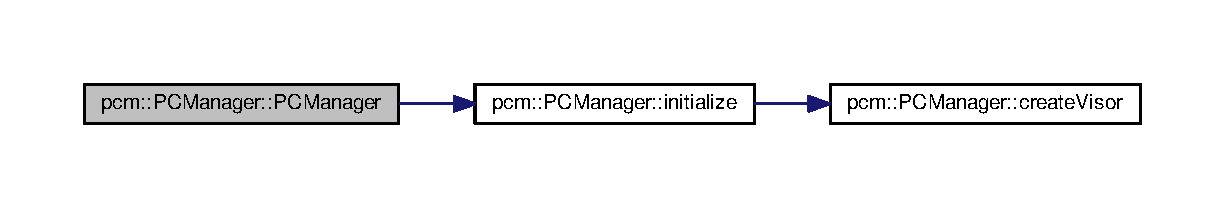
\includegraphics[width=350pt]{classpcm_1_1PCManager_ac9edd680fe7b6e9d8a2358ae8641759e_cgraph}
\end{center}
\end{figure}


\hypertarget{classpcm_1_1PCManager_af9dabc49537fa4521e7de8323a686856}{\index{pcm\-::\-P\-C\-Manager@{pcm\-::\-P\-C\-Manager}!P\-C\-Manager@{P\-C\-Manager}}
\index{P\-C\-Manager@{P\-C\-Manager}!pcm::PCManager@{pcm\-::\-P\-C\-Manager}}
\subsubsection[{P\-C\-Manager}]{\setlength{\rightskip}{0pt plus 5cm}pcm\-::\-P\-C\-Manager\-::\-P\-C\-Manager (
\begin{DoxyParamCaption}
\item[{bool}]{visualization\-Flag}
\end{DoxyParamCaption}
)}}\label{classpcm_1_1PCManager_af9dabc49537fa4521e7de8323a686856}


Definition at line 242 of file P\-C\-Manager.\-cpp.



References initialize().



Here is the call graph for this function\-:\nopagebreak
\begin{figure}[H]
\begin{center}
\leavevmode
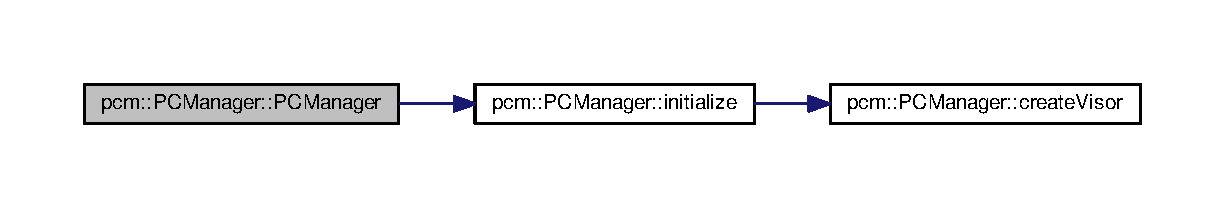
\includegraphics[width=350pt]{classpcm_1_1PCManager_af9dabc49537fa4521e7de8323a686856_cgraph}
\end{center}
\end{figure}


\hypertarget{classpcm_1_1PCManager_a488397e09fc7593a54d359ca899d6111}{\index{pcm\-::\-P\-C\-Manager@{pcm\-::\-P\-C\-Manager}!$\sim$\-P\-C\-Manager@{$\sim$\-P\-C\-Manager}}
\index{$\sim$\-P\-C\-Manager@{$\sim$\-P\-C\-Manager}!pcm::PCManager@{pcm\-::\-P\-C\-Manager}}
\subsubsection[{$\sim$\-P\-C\-Manager}]{\setlength{\rightskip}{0pt plus 5cm}pcm\-::\-P\-C\-Manager\-::$\sim$\-P\-C\-Manager (
\begin{DoxyParamCaption}
{}
\end{DoxyParamCaption}
)\hspace{0.3cm}{\ttfamily [virtual]}}}\label{classpcm_1_1PCManager_a488397e09fc7593a54d359ca899d6111}


Definition at line 247 of file P\-C\-Manager.\-cpp.



\subsection{Member Function Documentation}
\hypertarget{classpcm_1_1PCManager_a121d34f52021c5aed1e5133688df8774}{\index{pcm\-::\-P\-C\-Manager@{pcm\-::\-P\-C\-Manager}!add\-Primitive\-Shape@{add\-Primitive\-Shape}}
\index{add\-Primitive\-Shape@{add\-Primitive\-Shape}!pcm::PCManager@{pcm\-::\-P\-C\-Manager}}
\subsubsection[{add\-Primitive\-Shape}]{\setlength{\rightskip}{0pt plus 5cm}int pcm\-::\-P\-C\-Manager\-::add\-Primitive\-Shape (
\begin{DoxyParamCaption}
\item[{string}]{shape\-Name, }
\item[{{\bf P\-C\-L\-Cloud\-Ptr}}]{cloud, }
\item[{{\bf P\-C\-L\-Normal\-Ptr}}]{norms, }
\item[{bool}]{vis\-Flag}
\end{DoxyParamCaption}
)}}\label{classpcm_1_1PCManager_a121d34f52021c5aed1e5133688df8774}
\hypertarget{classpcm_1_1PCManager_a993ec5fee41e0ce3b4f9ce403c86aaec}{\index{pcm\-::\-P\-C\-Manager@{pcm\-::\-P\-C\-Manager}!clear\-Ptimitive\-Shape@{clear\-Ptimitive\-Shape}}
\index{clear\-Ptimitive\-Shape@{clear\-Ptimitive\-Shape}!pcm::PCManager@{pcm\-::\-P\-C\-Manager}}
\subsubsection[{clear\-Ptimitive\-Shape}]{\setlength{\rightskip}{0pt plus 5cm}int pcm\-::\-P\-C\-Manager\-::clear\-Ptimitive\-Shape (
\begin{DoxyParamCaption}
{}
\end{DoxyParamCaption}
)}}\label{classpcm_1_1PCManager_a993ec5fee41e0ce3b4f9ce403c86aaec}
\hypertarget{classpcm_1_1PCManager_a91753945c3d26f6aeee6f0dc6712a7fc}{\index{pcm\-::\-P\-C\-Manager@{pcm\-::\-P\-C\-Manager}!clear\-Visor@{clear\-Visor}}
\index{clear\-Visor@{clear\-Visor}!pcm::PCManager@{pcm\-::\-P\-C\-Manager}}
\subsubsection[{clear\-Visor}]{\setlength{\rightskip}{0pt plus 5cm}void pcm\-::\-P\-C\-Manager\-::clear\-Visor (
\begin{DoxyParamCaption}
\item[{{\bf P\-C\-L\-Visualizer}}]{viewer}
\end{DoxyParamCaption}
)\hspace{0.3cm}{\ttfamily [static]}}}\label{classpcm_1_1PCManager_a91753945c3d26f6aeee6f0dc6712a7fc}


Definition at line 179 of file P\-C\-Manager.\-cpp.

\hypertarget{classpcm_1_1PCManager_acb513ed7a3b898e398fd211bafac6f6a}{\index{pcm\-::\-P\-C\-Manager@{pcm\-::\-P\-C\-Manager}!cloud\-For\-Ros\-Msg@{cloud\-For\-Ros\-Msg}}
\index{cloud\-For\-Ros\-Msg@{cloud\-For\-Ros\-Msg}!pcm::PCManager@{pcm\-::\-P\-C\-Manager}}
\subsubsection[{cloud\-For\-Ros\-Msg}]{\setlength{\rightskip}{0pt plus 5cm}{\bf P\-C\-L\-Cloud\-Ptr} pcm\-::\-P\-C\-Manager\-::cloud\-For\-Ros\-Msg (
\begin{DoxyParamCaption}
\item[{Point\-Cloud2}]{input}
\end{DoxyParamCaption}
)\hspace{0.3cm}{\ttfamily [static]}}}\label{classpcm_1_1PCManager_acb513ed7a3b898e398fd211bafac6f6a}


Definition at line 101 of file P\-C\-Manager.\-cpp.



Referenced by clusterize(), ransac\-Cone\-Detaction(), ransac\-Cylinder\-Detaction(), ransac\-Plane\-Detaction(), ransac\-Sphere\-Detaction(), and set\-Original\-Cloud().

\hypertarget{classpcm_1_1PCManager_aea4756e187ee152c8695dc3e7496562e}{\index{pcm\-::\-P\-C\-Manager@{pcm\-::\-P\-C\-Manager}!cloud\-For\-Ros\-Msg@{cloud\-For\-Ros\-Msg}}
\index{cloud\-For\-Ros\-Msg@{cloud\-For\-Ros\-Msg}!pcm::PCManager@{pcm\-::\-P\-C\-Manager}}
\subsubsection[{cloud\-For\-Ros\-Msg}]{\setlength{\rightskip}{0pt plus 5cm}{\bf P\-C\-L\-Cloud\-Ptr} pcm\-::\-P\-C\-Manager\-::cloud\-For\-Ros\-Msg (
\begin{DoxyParamCaption}
\item[{Point\-Cloud2\-Ptr}]{input}
\end{DoxyParamCaption}
)\hspace{0.3cm}{\ttfamily [static]}}}\label{classpcm_1_1PCManager_aea4756e187ee152c8695dc3e7496562e}


Definition at line 96 of file P\-C\-Manager.\-cpp.

\hypertarget{classpcm_1_1PCManager_a9ec6cf99c0c34c9761fd923aace594dc}{\index{pcm\-::\-P\-C\-Manager@{pcm\-::\-P\-C\-Manager}!cloud\-To\-Ros\-Msg@{cloud\-To\-Ros\-Msg}}
\index{cloud\-To\-Ros\-Msg@{cloud\-To\-Ros\-Msg}!pcm::PCManager@{pcm\-::\-P\-C\-Manager}}
\subsubsection[{cloud\-To\-Ros\-Msg}]{\setlength{\rightskip}{0pt plus 5cm}Point\-Cloud2 pcm\-::\-P\-C\-Manager\-::cloud\-To\-Ros\-Msg (
\begin{DoxyParamCaption}
\item[{{\bf P\-C\-L\-Cloud\-Ptr}}]{input}
\end{DoxyParamCaption}
)\hspace{0.3cm}{\ttfamily [static]}}}\label{classpcm_1_1PCManager_a9ec6cf99c0c34c9761fd923aace594dc}


Definition at line 91 of file P\-C\-Manager.\-cpp.



Referenced by get\-Original\-Cloud\-Ros\-Msg().

\hypertarget{classpcm_1_1PCManager_a79353f94b8396268bea0a1358c260421}{\index{pcm\-::\-P\-C\-Manager@{pcm\-::\-P\-C\-Manager}!coefficient\-To\-Vector\-Msg@{coefficient\-To\-Vector\-Msg}}
\index{coefficient\-To\-Vector\-Msg@{coefficient\-To\-Vector\-Msg}!pcm::PCManager@{pcm\-::\-P\-C\-Manager}}
\subsubsection[{coefficient\-To\-Vector\-Msg}]{\setlength{\rightskip}{0pt plus 5cm}vector$<$ float $>$ pcm\-::\-P\-C\-Manager\-::coefficient\-To\-Vector\-Msg (
\begin{DoxyParamCaption}
\item[{Model\-Coefficients\-::\-Ptr}]{coefficients}
\end{DoxyParamCaption}
)\hspace{0.3cm}{\ttfamily [static]}}}\label{classpcm_1_1PCManager_a79353f94b8396268bea0a1358c260421}


Definition at line 123 of file P\-C\-Manager.\-cpp.



Referenced by ransac\-Cone\-Detaction(), ransac\-Cylinder\-Detaction(), ransac\-Plane\-Detaction(), and ransac\-Sphere\-Detaction().

\hypertarget{classpcm_1_1PCManager_afd0b3ae22849345d490ba27b425254a1}{\index{pcm\-::\-P\-C\-Manager@{pcm\-::\-P\-C\-Manager}!copy\-Cloud@{copy\-Cloud}}
\index{copy\-Cloud@{copy\-Cloud}!pcm::PCManager@{pcm\-::\-P\-C\-Manager}}
\subsubsection[{copy\-Cloud}]{\setlength{\rightskip}{0pt plus 5cm}{\bf P\-C\-L\-Cloud\-Ptr} pcm\-::\-P\-C\-Manager\-::copy\-Cloud (
\begin{DoxyParamCaption}
\item[{{\bf P\-C\-L\-Cloud\-Ptr}}]{input}
\end{DoxyParamCaption}
)\hspace{0.3cm}{\ttfamily [static]}}}\label{classpcm_1_1PCManager_afd0b3ae22849345d490ba27b425254a1}


Definition at line 41 of file P\-C\-Manager.\-cpp.

\hypertarget{classpcm_1_1PCManager_aa3397d6597a17ee15d2c539631e008c2}{\index{pcm\-::\-P\-C\-Manager@{pcm\-::\-P\-C\-Manager}!copy\-Coefficients@{copy\-Coefficients}}
\index{copy\-Coefficients@{copy\-Coefficients}!pcm::PCManager@{pcm\-::\-P\-C\-Manager}}
\subsubsection[{copy\-Coefficients}]{\setlength{\rightskip}{0pt plus 5cm}Model\-Coefficients\-::\-Ptr pcm\-::\-P\-C\-Manager\-::copy\-Coefficients (
\begin{DoxyParamCaption}
\item[{Model\-Coefficients\-::\-Ptr}]{input}
\end{DoxyParamCaption}
)\hspace{0.3cm}{\ttfamily [static]}}}\label{classpcm_1_1PCManager_aa3397d6597a17ee15d2c539631e008c2}


Definition at line 60 of file P\-C\-Manager.\-cpp.

\hypertarget{classpcm_1_1PCManager_aa580e879cf08a919167bcec0b213eb28}{\index{pcm\-::\-P\-C\-Manager@{pcm\-::\-P\-C\-Manager}!copy\-Normals@{copy\-Normals}}
\index{copy\-Normals@{copy\-Normals}!pcm::PCManager@{pcm\-::\-P\-C\-Manager}}
\subsubsection[{copy\-Normals}]{\setlength{\rightskip}{0pt plus 5cm}{\bf P\-C\-L\-Normal\-Ptr} pcm\-::\-P\-C\-Manager\-::copy\-Normals (
\begin{DoxyParamCaption}
\item[{{\bf P\-C\-L\-Normal\-Ptr}}]{input}
\end{DoxyParamCaption}
)\hspace{0.3cm}{\ttfamily [static]}}}\label{classpcm_1_1PCManager_aa580e879cf08a919167bcec0b213eb28}


Definition at line 54 of file P\-C\-Manager.\-cpp.

\hypertarget{classpcm_1_1PCManager_a23d8e95e891a3330785375e6672ec1fe}{\index{pcm\-::\-P\-C\-Manager@{pcm\-::\-P\-C\-Manager}!create\-Visor@{create\-Visor}}
\index{create\-Visor@{create\-Visor}!pcm::PCManager@{pcm\-::\-P\-C\-Manager}}
\subsubsection[{create\-Visor}]{\setlength{\rightskip}{0pt plus 5cm}{\bf P\-C\-L\-Visualizer} pcm\-::\-P\-C\-Manager\-::create\-Visor (
\begin{DoxyParamCaption}
\item[{string}]{title}
\end{DoxyParamCaption}
)\hspace{0.3cm}{\ttfamily [static]}}}\label{classpcm_1_1PCManager_a23d8e95e891a3330785375e6672ec1fe}


Definition at line 132 of file P\-C\-Manager.\-cpp.



Referenced by initialize(), main(), and set\-Visualization\-Flag().

\hypertarget{classpcm_1_1PCManager_ab9c66b0834ca1ef0c1c01e21400103dd}{\index{pcm\-::\-P\-C\-Manager@{pcm\-::\-P\-C\-Manager}!down\-Sampling@{down\-Sampling}}
\index{down\-Sampling@{down\-Sampling}!pcm::PCManager@{pcm\-::\-P\-C\-Manager}}
\subsubsection[{down\-Sampling}]{\setlength{\rightskip}{0pt plus 5cm}{\bf P\-C\-L\-Cloud\-Ptr} pcm\-::\-P\-C\-Manager\-::down\-Sampling (
\begin{DoxyParamCaption}
\item[{{\bf P\-C\-L\-Cloud\-Ptr}}]{input}
\end{DoxyParamCaption}
)\hspace{0.3cm}{\ttfamily [static]}}}\label{classpcm_1_1PCManager_ab9c66b0834ca1ef0c1c01e21400103dd}


Definition at line 66 of file P\-C\-Manager.\-cpp.



References D\-E\-F\-A\-U\-L\-T\-\_\-\-D\-O\-W\-S\-E\-A\-M\-P\-L\-I\-G\-\_\-\-R\-A\-T\-E.



Referenced by down\-Sampling(), and set\-Original\-Cloud().

\hypertarget{classpcm_1_1PCManager_a32a6c0ad1f2d23e48ddb4302be7d14c5}{\index{pcm\-::\-P\-C\-Manager@{pcm\-::\-P\-C\-Manager}!down\-Sampling@{down\-Sampling}}
\index{down\-Sampling@{down\-Sampling}!pcm::PCManager@{pcm\-::\-P\-C\-Manager}}
\subsubsection[{down\-Sampling}]{\setlength{\rightskip}{0pt plus 5cm}{\bf P\-C\-L\-Cloud\-Ptr} pcm\-::\-P\-C\-Manager\-::down\-Sampling (
\begin{DoxyParamCaption}
\item[{{\bf P\-C\-L\-Cloud\-Ptr}}]{input, }
\item[{float}]{span}
\end{DoxyParamCaption}
)\hspace{0.3cm}{\ttfamily [static]}}}\label{classpcm_1_1PCManager_a32a6c0ad1f2d23e48ddb4302be7d14c5}


Definition at line 69 of file P\-C\-Manager.\-cpp.



References down\-Sampling().



Here is the call graph for this function\-:\nopagebreak
\begin{figure}[H]
\begin{center}
\leavevmode
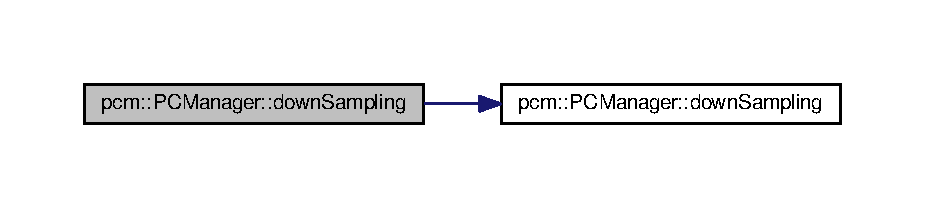
\includegraphics[width=350pt]{classpcm_1_1PCManager_a32a6c0ad1f2d23e48ddb4302be7d14c5_cgraph}
\end{center}
\end{figure}


\hypertarget{classpcm_1_1PCManager_a30723a3f4808cd2a161b58c0888d5dfa}{\index{pcm\-::\-P\-C\-Manager@{pcm\-::\-P\-C\-Manager}!down\-Sampling@{down\-Sampling}}
\index{down\-Sampling@{down\-Sampling}!pcm::PCManager@{pcm\-::\-P\-C\-Manager}}
\subsubsection[{down\-Sampling}]{\setlength{\rightskip}{0pt plus 5cm}{\bf P\-C\-L\-Cloud\-Ptr} pcm\-::\-P\-C\-Manager\-::down\-Sampling (
\begin{DoxyParamCaption}
\item[{{\bf P\-C\-L\-Cloud\-Ptr}}]{input, }
\item[{float}]{span\-X, }
\item[{float}]{span\-Y, }
\item[{float}]{span\-Z}
\end{DoxyParamCaption}
)\hspace{0.3cm}{\ttfamily [static]}}}\label{classpcm_1_1PCManager_a30723a3f4808cd2a161b58c0888d5dfa}


Definition at line 72 of file P\-C\-Manager.\-cpp.



References pcm\-::sor.

\hypertarget{classpcm_1_1PCManager_ab2cdef39cbe4f3d6c3660d873bd9a38e}{\index{pcm\-::\-P\-C\-Manager@{pcm\-::\-P\-C\-Manager}!estimate\-Normal@{estimate\-Normal}}
\index{estimate\-Normal@{estimate\-Normal}!pcm::PCManager@{pcm\-::\-P\-C\-Manager}}
\subsubsection[{estimate\-Normal}]{\setlength{\rightskip}{0pt plus 5cm}{\bf P\-C\-L\-Normal\-Ptr} pcm\-::\-P\-C\-Manager\-::estimate\-Normal (
\begin{DoxyParamCaption}
\item[{{\bf P\-C\-L\-Cloud\-Ptr}}]{input}
\end{DoxyParamCaption}
)\hspace{0.3cm}{\ttfamily [static]}}}\label{classpcm_1_1PCManager_ab2cdef39cbe4f3d6c3660d873bd9a38e}


Definition at line 79 of file P\-C\-Manager.\-cpp.



References D\-E\-F\-A\-U\-L\-T\-\_\-\-N\-O\-R\-M\-\_\-\-S\-E\-A\-R\-C\-H.



Referenced by set\-Original\-Cloud().

\hypertarget{classpcm_1_1PCManager_a7cad87bdc0a16f5b4b6108259ace90d3}{\index{pcm\-::\-P\-C\-Manager@{pcm\-::\-P\-C\-Manager}!estimate\-Normal@{estimate\-Normal}}
\index{estimate\-Normal@{estimate\-Normal}!pcm::PCManager@{pcm\-::\-P\-C\-Manager}}
\subsubsection[{estimate\-Normal}]{\setlength{\rightskip}{0pt plus 5cm}{\bf P\-C\-L\-Normal\-Ptr} pcm\-::\-P\-C\-Manager\-::estimate\-Normal (
\begin{DoxyParamCaption}
\item[{{\bf P\-C\-L\-Cloud\-Ptr}}]{input, }
\item[{int}]{search}
\end{DoxyParamCaption}
)\hspace{0.3cm}{\ttfamily [static]}}}\label{classpcm_1_1PCManager_a7cad87bdc0a16f5b4b6108259ace90d3}


Definition at line 82 of file P\-C\-Manager.\-cpp.



References pcm\-::ne, and pcm\-::tree().



Here is the call graph for this function\-:\nopagebreak
\begin{figure}[H]
\begin{center}
\leavevmode
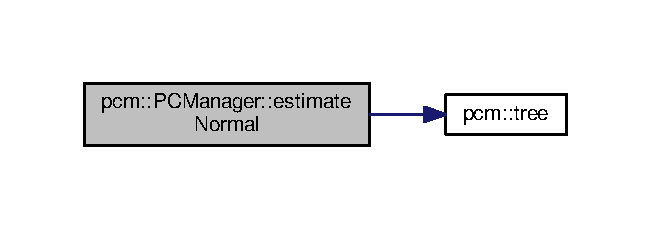
\includegraphics[width=312pt]{classpcm_1_1PCManager_a7cad87bdc0a16f5b4b6108259ace90d3_cgraph}
\end{center}
\end{figure}


\hypertarget{classpcm_1_1PCManager_a881ed083a239069699906a669492fc1d}{\index{pcm\-::\-P\-C\-Manager@{pcm\-::\-P\-C\-Manager}!get\-Cloud\-From\-Idx@{get\-Cloud\-From\-Idx}}
\index{get\-Cloud\-From\-Idx@{get\-Cloud\-From\-Idx}!pcm::PCManager@{pcm\-::\-P\-C\-Manager}}
\subsubsection[{get\-Cloud\-From\-Idx}]{\setlength{\rightskip}{0pt plus 5cm}vector$<$ {\bf P\-C\-L\-Cloud\-Ptr} $>$ pcm\-::\-P\-C\-Manager\-::get\-Cloud\-From\-Idx (
\begin{DoxyParamCaption}
\item[{{\bf P\-C\-L\-Cloud\-Ptr}}]{original\-Cloud, }
\item[{{\bf Primitive\-Idx\-Ptr}}]{indices}
\end{DoxyParamCaption}
)\hspace{0.3cm}{\ttfamily [static]}}}\label{classpcm_1_1PCManager_a881ed083a239069699906a669492fc1d}


Definition at line 185 of file P\-C\-Manager.\-cpp.



Referenced by get\-Cloud\-From\-Idx().

\hypertarget{classpcm_1_1PCManager_a73da6d454214f5ba90d978b50ff4438f}{\index{pcm\-::\-P\-C\-Manager@{pcm\-::\-P\-C\-Manager}!get\-Cloud\-From\-Idx@{get\-Cloud\-From\-Idx}}
\index{get\-Cloud\-From\-Idx@{get\-Cloud\-From\-Idx}!pcm::PCManager@{pcm\-::\-P\-C\-Manager}}
\subsubsection[{get\-Cloud\-From\-Idx}]{\setlength{\rightskip}{0pt plus 5cm}vector$<$ {\bf P\-C\-L\-Cloud\-Ptr} $>$ pcm\-::\-P\-C\-Manager\-::get\-Cloud\-From\-Idx (
\begin{DoxyParamCaption}
\item[{{\bf Primitive\-Idx\-Ptr}}]{indices}
\end{DoxyParamCaption}
)}}\label{classpcm_1_1PCManager_a73da6d454214f5ba90d978b50ff4438f}


Definition at line 231 of file P\-C\-Manager.\-cpp.



References get\-Cloud\-From\-Idx(), and original\-Cloud.



Here is the call graph for this function\-:\nopagebreak
\begin{figure}[H]
\begin{center}
\leavevmode
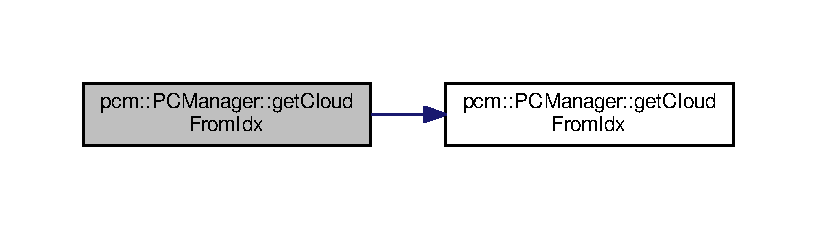
\includegraphics[width=350pt]{classpcm_1_1PCManager_a73da6d454214f5ba90d978b50ff4438f_cgraph}
\end{center}
\end{figure}


\hypertarget{classpcm_1_1PCManager_a3f26dafa3a2808b3ee927d9724f9c9a6}{\index{pcm\-::\-P\-C\-Manager@{pcm\-::\-P\-C\-Manager}!get\-Original\-Cloud@{get\-Original\-Cloud}}
\index{get\-Original\-Cloud@{get\-Original\-Cloud}!pcm::PCManager@{pcm\-::\-P\-C\-Manager}}
\subsubsection[{get\-Original\-Cloud}]{\setlength{\rightskip}{0pt plus 5cm}{\bf P\-C\-L\-Cloud\-Ptr} pcm\-::\-P\-C\-Manager\-::get\-Original\-Cloud (
\begin{DoxyParamCaption}
{}
\end{DoxyParamCaption}
)}}\label{classpcm_1_1PCManager_a3f26dafa3a2808b3ee927d9724f9c9a6}


Definition at line 285 of file P\-C\-Manager.\-cpp.



References original\-Cloud.

\hypertarget{classpcm_1_1PCManager_a1a11270e78e96c38f9c40985529fc5b6}{\index{pcm\-::\-P\-C\-Manager@{pcm\-::\-P\-C\-Manager}!get\-Original\-Cloud\-Ros\-Msg@{get\-Original\-Cloud\-Ros\-Msg}}
\index{get\-Original\-Cloud\-Ros\-Msg@{get\-Original\-Cloud\-Ros\-Msg}!pcm::PCManager@{pcm\-::\-P\-C\-Manager}}
\subsubsection[{get\-Original\-Cloud\-Ros\-Msg}]{\setlength{\rightskip}{0pt plus 5cm}Point\-Cloud2 pcm\-::\-P\-C\-Manager\-::get\-Original\-Cloud\-Ros\-Msg (
\begin{DoxyParamCaption}
{}
\end{DoxyParamCaption}
)}}\label{classpcm_1_1PCManager_a1a11270e78e96c38f9c40985529fc5b6}


Definition at line 288 of file P\-C\-Manager.\-cpp.



References cloud\-To\-Ros\-Msg(), and original\-Cloud.



Here is the call graph for this function\-:\nopagebreak
\begin{figure}[H]
\begin{center}
\leavevmode
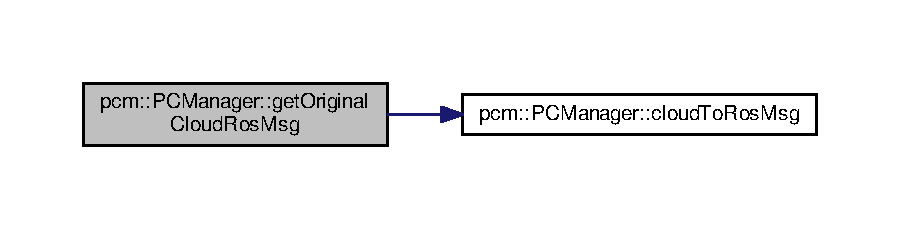
\includegraphics[width=350pt]{classpcm_1_1PCManager_a1a11270e78e96c38f9c40985529fc5b6_cgraph}
\end{center}
\end{figure}


\hypertarget{classpcm_1_1PCManager_a471d768a4a32a8d8992c688fc6fc2f58}{\index{pcm\-::\-P\-C\-Manager@{pcm\-::\-P\-C\-Manager}!get\-Original\-Normal@{get\-Original\-Normal}}
\index{get\-Original\-Normal@{get\-Original\-Normal}!pcm::PCManager@{pcm\-::\-P\-C\-Manager}}
\subsubsection[{get\-Original\-Normal}]{\setlength{\rightskip}{0pt plus 5cm}{\bf P\-C\-L\-Normal\-Ptr} pcm\-::\-P\-C\-Manager\-::get\-Original\-Normal (
\begin{DoxyParamCaption}
{}
\end{DoxyParamCaption}
)}}\label{classpcm_1_1PCManager_a471d768a4a32a8d8992c688fc6fc2f58}


Definition at line 292 of file P\-C\-Manager.\-cpp.



References original\-Norms.

\hypertarget{classpcm_1_1PCManager_a01a64a81b18e5bc984c46910d2a881be}{\index{pcm\-::\-P\-C\-Manager@{pcm\-::\-P\-C\-Manager}!get\-Original\-Normal\-Ros\-Msg@{get\-Original\-Normal\-Ros\-Msg}}
\index{get\-Original\-Normal\-Ros\-Msg@{get\-Original\-Normal\-Ros\-Msg}!pcm::PCManager@{pcm\-::\-P\-C\-Manager}}
\subsubsection[{get\-Original\-Normal\-Ros\-Msg}]{\setlength{\rightskip}{0pt plus 5cm}Point\-Cloud2 pcm\-::\-P\-C\-Manager\-::get\-Original\-Normal\-Ros\-Msg (
\begin{DoxyParamCaption}
{}
\end{DoxyParamCaption}
)}}\label{classpcm_1_1PCManager_a01a64a81b18e5bc984c46910d2a881be}


Definition at line 295 of file P\-C\-Manager.\-cpp.



References norm\-To\-Ros\-Msg(), and original\-Norms.



Here is the call graph for this function\-:\nopagebreak
\begin{figure}[H]
\begin{center}
\leavevmode
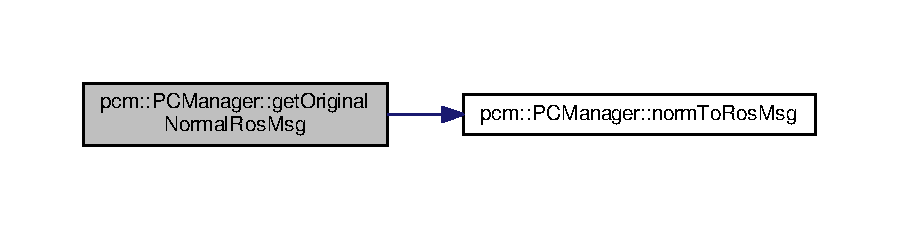
\includegraphics[width=350pt]{classpcm_1_1PCManager_a01a64a81b18e5bc984c46910d2a881be_cgraph}
\end{center}
\end{figure}


\hypertarget{classpcm_1_1PCManager_a3575801a21b3fd9613dd57cb97ffaa47}{\index{pcm\-::\-P\-C\-Manager@{pcm\-::\-P\-C\-Manager}!get\-Primitive\-Shape@{get\-Primitive\-Shape}}
\index{get\-Primitive\-Shape@{get\-Primitive\-Shape}!pcm::PCManager@{pcm\-::\-P\-C\-Manager}}
\subsubsection[{get\-Primitive\-Shape}]{\setlength{\rightskip}{0pt plus 5cm}{\bf P\-C\-Primitive\-Ptr} pcm\-::\-P\-C\-Manager\-::get\-Primitive\-Shape (
\begin{DoxyParamCaption}
\item[{int}]{idx}
\end{DoxyParamCaption}
)}}\label{classpcm_1_1PCManager_a3575801a21b3fd9613dd57cb97ffaa47}
\hypertarget{classpcm_1_1PCManager_ac1cfd8753c305e761a3c5914f74cca7b}{\index{pcm\-::\-P\-C\-Manager@{pcm\-::\-P\-C\-Manager}!get\-Visor@{get\-Visor}}
\index{get\-Visor@{get\-Visor}!pcm::PCManager@{pcm\-::\-P\-C\-Manager}}
\subsubsection[{get\-Visor}]{\setlength{\rightskip}{0pt plus 5cm}{\bf P\-C\-L\-Visualizer} pcm\-::\-P\-C\-Manager\-::get\-Visor (
\begin{DoxyParamCaption}
{}
\end{DoxyParamCaption}
)}}\label{classpcm_1_1PCManager_ac1cfd8753c305e761a3c5914f74cca7b}


Definition at line 302 of file P\-C\-Manager.\-cpp.



References visor.

\hypertarget{classpcm_1_1PCManager_a4d419e1bf7e35f8f3ddbb7f640c50a72}{\index{pcm\-::\-P\-C\-Manager@{pcm\-::\-P\-C\-Manager}!get\-Visualization\-Flag@{get\-Visualization\-Flag}}
\index{get\-Visualization\-Flag@{get\-Visualization\-Flag}!pcm::PCManager@{pcm\-::\-P\-C\-Manager}}
\subsubsection[{get\-Visualization\-Flag}]{\setlength{\rightskip}{0pt plus 5cm}bool pcm\-::\-P\-C\-Manager\-::get\-Visualization\-Flag (
\begin{DoxyParamCaption}
{}
\end{DoxyParamCaption}
)}}\label{classpcm_1_1PCManager_a4d419e1bf7e35f8f3ddbb7f640c50a72}


Definition at line 299 of file P\-C\-Manager.\-cpp.



References visualization\-Flag.

\hypertarget{classpcm_1_1PCManager_ad79130d97fa80234552372c3e7e81ee3}{\index{pcm\-::\-P\-C\-Manager@{pcm\-::\-P\-C\-Manager}!initialize@{initialize}}
\index{initialize@{initialize}!pcm::PCManager@{pcm\-::\-P\-C\-Manager}}
\subsubsection[{initialize}]{\setlength{\rightskip}{0pt plus 5cm}void pcm\-::\-P\-C\-Manager\-::initialize (
\begin{DoxyParamCaption}
\item[{bool}]{visualization\-Flag}
\end{DoxyParamCaption}
)\hspace{0.3cm}{\ttfamily [private]}}}\label{classpcm_1_1PCManager_ad79130d97fa80234552372c3e7e81ee3}


Definition at line 343 of file P\-C\-Manager.\-cpp.



References create\-Visor(), D\-E\-F\-A\-U\-L\-T\-\_\-\-V\-I\-S\-U\-A\-L\-I\-Z\-E\-R\-\_\-\-T\-I\-T\-L\-E, visor, and visualization\-Flag.



Referenced by P\-C\-Manager().



Here is the call graph for this function\-:\nopagebreak
\begin{figure}[H]
\begin{center}
\leavevmode
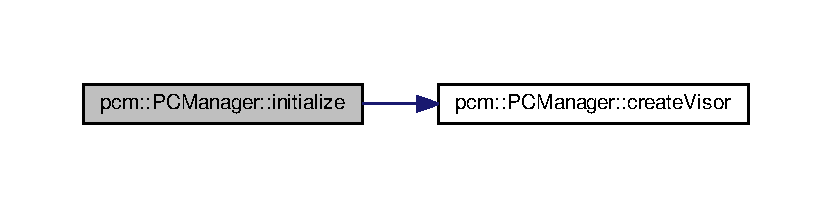
\includegraphics[width=350pt]{classpcm_1_1PCManager_ad79130d97fa80234552372c3e7e81ee3_cgraph}
\end{center}
\end{figure}


\hypertarget{classpcm_1_1PCManager_ab473f60dc622465a1c3ff77000f0803f}{\index{pcm\-::\-P\-C\-Manager@{pcm\-::\-P\-C\-Manager}!inlier\-To\-Vector\-Msg@{inlier\-To\-Vector\-Msg}}
\index{inlier\-To\-Vector\-Msg@{inlier\-To\-Vector\-Msg}!pcm::PCManager@{pcm\-::\-P\-C\-Manager}}
\subsubsection[{inlier\-To\-Vector\-Msg}]{\setlength{\rightskip}{0pt plus 5cm}vector$<$ int $>$ pcm\-::\-P\-C\-Manager\-::inlier\-To\-Vector\-Msg (
\begin{DoxyParamCaption}
\item[{Point\-Indices\-::\-Ptr}]{inliers}
\end{DoxyParamCaption}
)\hspace{0.3cm}{\ttfamily [static]}}}\label{classpcm_1_1PCManager_ab473f60dc622465a1c3ff77000f0803f}


Definition at line 116 of file P\-C\-Manager.\-cpp.



Referenced by ransac\-Cone\-Detaction(), ransac\-Cylinder\-Detaction(), ransac\-Plane\-Detaction(), and ransac\-Sphere\-Detaction().

\hypertarget{classpcm_1_1PCManager_a75f790855ce87d24293bb3a8e4a453c9}{\index{pcm\-::\-P\-C\-Manager@{pcm\-::\-P\-C\-Manager}!norm\-For\-Ros\-Msg@{norm\-For\-Ros\-Msg}}
\index{norm\-For\-Ros\-Msg@{norm\-For\-Ros\-Msg}!pcm::PCManager@{pcm\-::\-P\-C\-Manager}}
\subsubsection[{norm\-For\-Ros\-Msg}]{\setlength{\rightskip}{0pt plus 5cm}{\bf P\-C\-L\-Normal\-Ptr} pcm\-::\-P\-C\-Manager\-::norm\-For\-Ros\-Msg (
\begin{DoxyParamCaption}
\item[{Point\-Cloud2}]{input}
\end{DoxyParamCaption}
)\hspace{0.3cm}{\ttfamily [static]}}}\label{classpcm_1_1PCManager_a75f790855ce87d24293bb3a8e4a453c9}


Definition at line 111 of file P\-C\-Manager.\-cpp.



Referenced by ransac\-Cone\-Detaction(), ransac\-Cylinder\-Detaction(), ransac\-Plane\-Detaction(), and ransac\-Sphere\-Detaction().

\hypertarget{classpcm_1_1PCManager_aad8d4dd6c1bb761213134760be5673c3}{\index{pcm\-::\-P\-C\-Manager@{pcm\-::\-P\-C\-Manager}!norm\-To\-Ros\-Msg@{norm\-To\-Ros\-Msg}}
\index{norm\-To\-Ros\-Msg@{norm\-To\-Ros\-Msg}!pcm::PCManager@{pcm\-::\-P\-C\-Manager}}
\subsubsection[{norm\-To\-Ros\-Msg}]{\setlength{\rightskip}{0pt plus 5cm}Point\-Cloud2 pcm\-::\-P\-C\-Manager\-::norm\-To\-Ros\-Msg (
\begin{DoxyParamCaption}
\item[{{\bf P\-C\-L\-Normal\-Ptr}}]{input}
\end{DoxyParamCaption}
)\hspace{0.3cm}{\ttfamily [static]}}}\label{classpcm_1_1PCManager_aad8d4dd6c1bb761213134760be5673c3}


Definition at line 106 of file P\-C\-Manager.\-cpp.



Referenced by get\-Original\-Normal\-Ros\-Msg().

\hypertarget{classpcm_1_1PCManager_a2144cf37b92d58e902f7e6b1dcb6984d}{\index{pcm\-::\-P\-C\-Manager@{pcm\-::\-P\-C\-Manager}!set\-Original\-Cloud@{set\-Original\-Cloud}}
\index{set\-Original\-Cloud@{set\-Original\-Cloud}!pcm::PCManager@{pcm\-::\-P\-C\-Manager}}
\subsubsection[{set\-Original\-Cloud}]{\setlength{\rightskip}{0pt plus 5cm}void pcm\-::\-P\-C\-Manager\-::set\-Original\-Cloud (
\begin{DoxyParamCaption}
\item[{{\bf P\-C\-L\-Cloud\-Ptr}}]{cloud}
\end{DoxyParamCaption}
)}}\label{classpcm_1_1PCManager_a2144cf37b92d58e902f7e6b1dcb6984d}


Definition at line 308 of file P\-C\-Manager.\-cpp.



References D\-E\-F\-A\-U\-L\-T\-\_\-\-D\-O\-W\-S\-E\-A\-M\-P\-L\-I\-G\-\_\-\-R\-A\-T\-E, and D\-E\-F\-A\-U\-L\-T\-\_\-\-N\-O\-R\-M\-\_\-\-S\-E\-A\-R\-C\-H.



Referenced by set\-Original\-Cloud().

\hypertarget{classpcm_1_1PCManager_ac277411304ee22415cdeaad26cd4721c}{\index{pcm\-::\-P\-C\-Manager@{pcm\-::\-P\-C\-Manager}!set\-Original\-Cloud@{set\-Original\-Cloud}}
\index{set\-Original\-Cloud@{set\-Original\-Cloud}!pcm::PCManager@{pcm\-::\-P\-C\-Manager}}
\subsubsection[{set\-Original\-Cloud}]{\setlength{\rightskip}{0pt plus 5cm}void pcm\-::\-P\-C\-Manager\-::set\-Original\-Cloud (
\begin{DoxyParamCaption}
\item[{{\bf P\-C\-L\-Cloud\-Ptr}}]{cloud, }
\item[{int}]{norm\-Search, }
\item[{float}]{down\-Span\-X, }
\item[{float}]{down\-Span\-Y, }
\item[{float}]{down\-Span\-Z}
\end{DoxyParamCaption}
)}}\label{classpcm_1_1PCManager_ac277411304ee22415cdeaad26cd4721c}


Definition at line 311 of file P\-C\-Manager.\-cpp.



References down\-Sampling(), estimate\-Normal(), original\-Cloud, and original\-Norms.



Here is the call graph for this function\-:\nopagebreak
\begin{figure}[H]
\begin{center}
\leavevmode
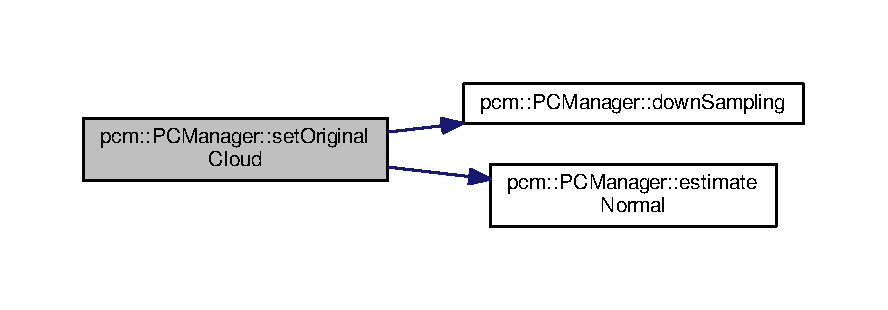
\includegraphics[width=350pt]{classpcm_1_1PCManager_ac277411304ee22415cdeaad26cd4721c_cgraph}
\end{center}
\end{figure}


\hypertarget{classpcm_1_1PCManager_a8eafedbcc9cb93380e826bc45bff1410}{\index{pcm\-::\-P\-C\-Manager@{pcm\-::\-P\-C\-Manager}!set\-Original\-Cloud@{set\-Original\-Cloud}}
\index{set\-Original\-Cloud@{set\-Original\-Cloud}!pcm::PCManager@{pcm\-::\-P\-C\-Manager}}
\subsubsection[{set\-Original\-Cloud}]{\setlength{\rightskip}{0pt plus 5cm}void pcm\-::\-P\-C\-Manager\-::set\-Original\-Cloud (
\begin{DoxyParamCaption}
\item[{Point\-Cloud2\-Ptr}]{cloud}
\end{DoxyParamCaption}
)}}\label{classpcm_1_1PCManager_a8eafedbcc9cb93380e826bc45bff1410}


Definition at line 319 of file P\-C\-Manager.\-cpp.



References D\-E\-F\-A\-U\-L\-T\-\_\-\-D\-O\-W\-S\-E\-A\-M\-P\-L\-I\-G\-\_\-\-R\-A\-T\-E, D\-E\-F\-A\-U\-L\-T\-\_\-\-N\-O\-R\-M\-\_\-\-S\-E\-A\-R\-C\-H, and set\-Original\-Cloud().



Here is the call graph for this function\-:\nopagebreak
\begin{figure}[H]
\begin{center}
\leavevmode
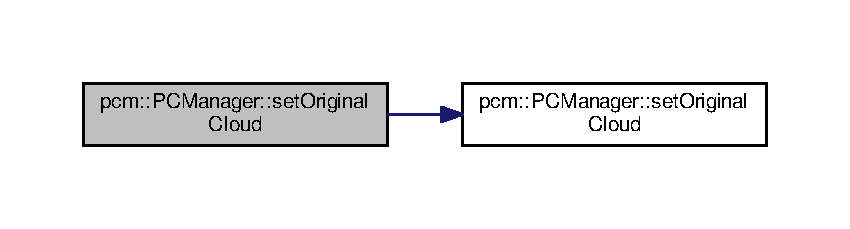
\includegraphics[width=350pt]{classpcm_1_1PCManager_a8eafedbcc9cb93380e826bc45bff1410_cgraph}
\end{center}
\end{figure}


\hypertarget{classpcm_1_1PCManager_aa5bd3ef55ff3ef39cded25351c7b4d9e}{\index{pcm\-::\-P\-C\-Manager@{pcm\-::\-P\-C\-Manager}!set\-Original\-Cloud@{set\-Original\-Cloud}}
\index{set\-Original\-Cloud@{set\-Original\-Cloud}!pcm::PCManager@{pcm\-::\-P\-C\-Manager}}
\subsubsection[{set\-Original\-Cloud}]{\setlength{\rightskip}{0pt plus 5cm}void pcm\-::\-P\-C\-Manager\-::set\-Original\-Cloud (
\begin{DoxyParamCaption}
\item[{Point\-Cloud2\-Ptr}]{cloud, }
\item[{int}]{norm\-Search, }
\item[{float}]{down\-Span\-X, }
\item[{float}]{down\-Span\-Y, }
\item[{float}]{down\-Span\-Z}
\end{DoxyParamCaption}
)}}\label{classpcm_1_1PCManager_aa5bd3ef55ff3ef39cded25351c7b4d9e}


Definition at line 322 of file P\-C\-Manager.\-cpp.



References cloud\-For\-Ros\-Msg(), and set\-Original\-Cloud().



Here is the call graph for this function\-:\nopagebreak
\begin{figure}[H]
\begin{center}
\leavevmode
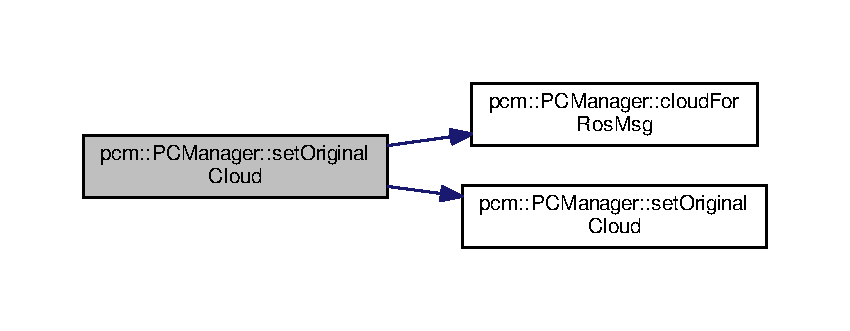
\includegraphics[width=350pt]{classpcm_1_1PCManager_aa5bd3ef55ff3ef39cded25351c7b4d9e_cgraph}
\end{center}
\end{figure}


\hypertarget{classpcm_1_1PCManager_a40c79e3197147779d263b95fd3617974}{\index{pcm\-::\-P\-C\-Manager@{pcm\-::\-P\-C\-Manager}!set\-Visualization\-Flag@{set\-Visualization\-Flag}}
\index{set\-Visualization\-Flag@{set\-Visualization\-Flag}!pcm::PCManager@{pcm\-::\-P\-C\-Manager}}
\subsubsection[{set\-Visualization\-Flag}]{\setlength{\rightskip}{0pt plus 5cm}void pcm\-::\-P\-C\-Manager\-::set\-Visualization\-Flag (
\begin{DoxyParamCaption}
\item[{bool}]{flag}
\end{DoxyParamCaption}
)}}\label{classpcm_1_1PCManager_a40c79e3197147779d263b95fd3617974}


Definition at line 326 of file P\-C\-Manager.\-cpp.



References create\-Visor(), D\-E\-F\-A\-U\-L\-T\-\_\-\-V\-I\-S\-U\-A\-L\-I\-Z\-E\-R\-\_\-\-T\-I\-T\-L\-E, visor, and visualization\-Flag.



Here is the call graph for this function\-:\nopagebreak
\begin{figure}[H]
\begin{center}
\leavevmode
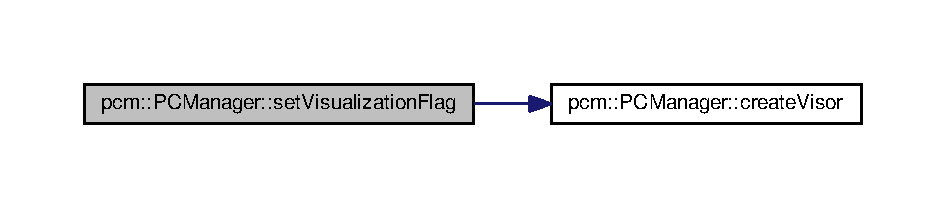
\includegraphics[width=350pt]{classpcm_1_1PCManager_a40c79e3197147779d263b95fd3617974_cgraph}
\end{center}
\end{figure}


\hypertarget{classpcm_1_1PCManager_a8b6dfcce0709c29f63a82c4dfa6ef6e6}{\index{pcm\-::\-P\-C\-Manager@{pcm\-::\-P\-C\-Manager}!update\-Visor@{update\-Visor}}
\index{update\-Visor@{update\-Visor}!pcm::PCManager@{pcm\-::\-P\-C\-Manager}}
\subsubsection[{update\-Visor}]{\setlength{\rightskip}{0pt plus 5cm}void pcm\-::\-P\-C\-Manager\-::update\-Visor (
\begin{DoxyParamCaption}
\item[{{\bf P\-C\-L\-Visualizer}}]{viewer, }
\item[{{\bf P\-C\-L\-Cloud\-Ptr}}]{cloud, }
\item[{int}]{R, }
\item[{int}]{G, }
\item[{int}]{B, }
\item[{string}]{name}
\end{DoxyParamCaption}
)\hspace{0.3cm}{\ttfamily [static]}}}\label{classpcm_1_1PCManager_a8b6dfcce0709c29f63a82c4dfa6ef6e6}


Definition at line 154 of file P\-C\-Manager.\-cpp.



References V\-I\-S\-U\-A\-L\-I\-Z\-E\-R\-\_\-\-P\-O\-I\-N\-T\-\_\-\-S\-I\-Z\-E.



Referenced by ransac\-Cone\-Detaction(), ransac\-Cylinder\-Detaction(), and update\-Visor().

\hypertarget{classpcm_1_1PCManager_af6498d518bd4eb1ad5f724849a851e90}{\index{pcm\-::\-P\-C\-Manager@{pcm\-::\-P\-C\-Manager}!update\-Visor@{update\-Visor}}
\index{update\-Visor@{update\-Visor}!pcm::PCManager@{pcm\-::\-P\-C\-Manager}}
\subsubsection[{update\-Visor}]{\setlength{\rightskip}{0pt plus 5cm}void pcm\-::\-P\-C\-Manager\-::update\-Visor (
\begin{DoxyParamCaption}
\item[{{\bf P\-C\-L\-Visualizer}}]{viewer, }
\item[{{\bf P\-C\-L\-Cloud\-Ptr}}]{cloud, }
\item[{string}]{name}
\end{DoxyParamCaption}
)\hspace{0.3cm}{\ttfamily [static]}}}\label{classpcm_1_1PCManager_af6498d518bd4eb1ad5f724849a851e90}


Definition at line 162 of file P\-C\-Manager.\-cpp.



References update\-Visor().



Here is the call graph for this function\-:\nopagebreak
\begin{figure}[H]
\begin{center}
\leavevmode
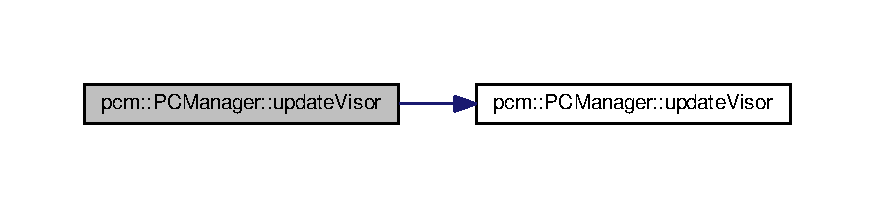
\includegraphics[width=350pt]{classpcm_1_1PCManager_af6498d518bd4eb1ad5f724849a851e90_cgraph}
\end{center}
\end{figure}


\hypertarget{classpcm_1_1PCManager_ae65d976eaaf49a2db303e91d30279cb0}{\index{pcm\-::\-P\-C\-Manager@{pcm\-::\-P\-C\-Manager}!update\-Visor@{update\-Visor}}
\index{update\-Visor@{update\-Visor}!pcm::PCManager@{pcm\-::\-P\-C\-Manager}}
\subsubsection[{update\-Visor}]{\setlength{\rightskip}{0pt plus 5cm}void pcm\-::\-P\-C\-Manager\-::update\-Visor (
\begin{DoxyParamCaption}
\item[{{\bf P\-C\-L\-Visualizer}}]{viewer, }
\item[{{\bf P\-C\-L\-Cloud\-Ptr}}]{cloud, }
\item[{{\bf P\-C\-L\-Normal\-Ptr}}]{normals, }
\item[{int}]{R, }
\item[{int}]{G, }
\item[{int}]{B, }
\item[{string}]{name}
\end{DoxyParamCaption}
)\hspace{0.3cm}{\ttfamily [static]}}}\label{classpcm_1_1PCManager_ae65d976eaaf49a2db303e91d30279cb0}


Definition at line 166 of file P\-C\-Manager.\-cpp.



References D\-E\-F\-A\-U\-L\-T\-\_\-\-N\-O\-R\-M\-\_\-\-L\-E\-V\-E\-L, D\-E\-F\-A\-U\-L\-T\-\_\-\-N\-O\-R\-M\-\_\-\-N\-A\-M\-E\-\_\-\-S\-U\-F\-F\-I\-X, D\-E\-F\-A\-U\-L\-T\-\_\-\-N\-O\-R\-M\-\_\-\-S\-C\-A\-L\-E, and V\-I\-S\-U\-A\-L\-I\-Z\-E\-R\-\_\-\-P\-O\-I\-N\-T\-\_\-\-S\-I\-Z\-E.

\hypertarget{classpcm_1_1PCManager_a183ac77330de59a04c4de18e3270fbb8}{\index{pcm\-::\-P\-C\-Manager@{pcm\-::\-P\-C\-Manager}!update\-Visor@{update\-Visor}}
\index{update\-Visor@{update\-Visor}!pcm::PCManager@{pcm\-::\-P\-C\-Manager}}
\subsubsection[{update\-Visor}]{\setlength{\rightskip}{0pt plus 5cm}void pcm\-::\-P\-C\-Manager\-::update\-Visor (
\begin{DoxyParamCaption}
\item[{{\bf P\-C\-L\-Visualizer}}]{viewer, }
\item[{{\bf P\-C\-L\-Cloud\-Ptr}}]{cloud, }
\item[{{\bf P\-C\-L\-Normal\-Ptr}}]{normals, }
\item[{string}]{name}
\end{DoxyParamCaption}
)\hspace{0.3cm}{\ttfamily [static]}}}\label{classpcm_1_1PCManager_a183ac77330de59a04c4de18e3270fbb8}


Definition at line 176 of file P\-C\-Manager.\-cpp.



References update\-Visor().



Here is the call graph for this function\-:\nopagebreak
\begin{figure}[H]
\begin{center}
\leavevmode
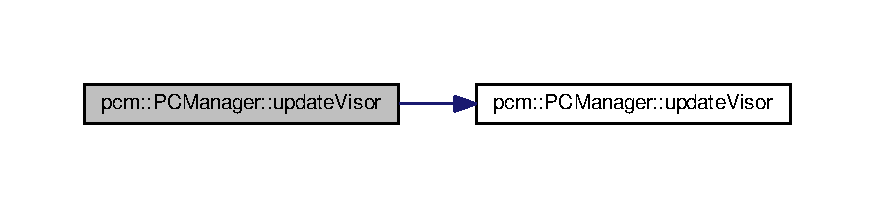
\includegraphics[width=350pt]{classpcm_1_1PCManager_a183ac77330de59a04c4de18e3270fbb8_cgraph}
\end{center}
\end{figure}


\hypertarget{classpcm_1_1PCManager_a4e249a3ef952e13bf941ccb90ff6c1f9}{\index{pcm\-::\-P\-C\-Manager@{pcm\-::\-P\-C\-Manager}!update\-Visor@{update\-Visor}}
\index{update\-Visor@{update\-Visor}!pcm::PCManager@{pcm\-::\-P\-C\-Manager}}
\subsubsection[{update\-Visor}]{\setlength{\rightskip}{0pt plus 5cm}void pcm\-::\-P\-C\-Manager\-::update\-Visor (
\begin{DoxyParamCaption}
\item[{{\bf P\-C\-L\-Visualizer}}]{viewer, }
\item[{Point\-X\-Y\-Z}]{point, }
\item[{int}]{R, }
\item[{int}]{G, }
\item[{int}]{B, }
\item[{string}]{name}
\end{DoxyParamCaption}
)\hspace{0.3cm}{\ttfamily [static]}}}\label{classpcm_1_1PCManager_a4e249a3ef952e13bf941ccb90ff6c1f9}


Definition at line 140 of file P\-C\-Manager.\-cpp.



References V\-I\-S\-U\-A\-L\-I\-Z\-E\-R\-\_\-\-P\-O\-I\-N\-T\-\_\-\-S\-I\-Z\-E\-\_\-\-B\-I\-G.

\hypertarget{classpcm_1_1PCManager_a684c37d6b0637aa3bb08fe47d67b9fb6}{\index{pcm\-::\-P\-C\-Manager@{pcm\-::\-P\-C\-Manager}!update\-Visor@{update\-Visor}}
\index{update\-Visor@{update\-Visor}!pcm::PCManager@{pcm\-::\-P\-C\-Manager}}
\subsubsection[{update\-Visor}]{\setlength{\rightskip}{0pt plus 5cm}void pcm\-::\-P\-C\-Manager\-::update\-Visor (
\begin{DoxyParamCaption}
\item[{{\bf P\-C\-L\-Visualizer}}]{viewer, }
\item[{Point\-X\-Y\-Z}]{point, }
\item[{string}]{name}
\end{DoxyParamCaption}
)\hspace{0.3cm}{\ttfamily [static]}}}\label{classpcm_1_1PCManager_a684c37d6b0637aa3bb08fe47d67b9fb6}


Definition at line 150 of file P\-C\-Manager.\-cpp.



References update\-Visor().



Here is the call graph for this function\-:\nopagebreak
\begin{figure}[H]
\begin{center}
\leavevmode
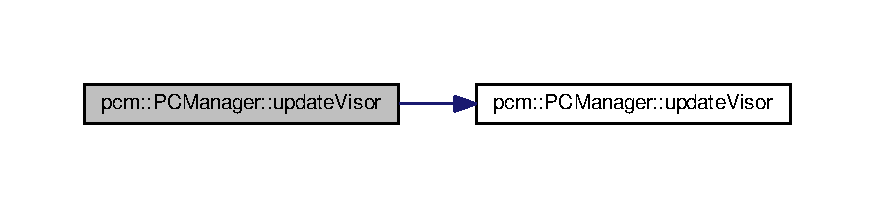
\includegraphics[width=350pt]{classpcm_1_1PCManager_a684c37d6b0637aa3bb08fe47d67b9fb6_cgraph}
\end{center}
\end{figure}


\hypertarget{classpcm_1_1PCManager_ad73afae724cbba84e40ed94ac4123864}{\index{pcm\-::\-P\-C\-Manager@{pcm\-::\-P\-C\-Manager}!visualize@{visualize}}
\index{visualize@{visualize}!pcm::PCManager@{pcm\-::\-P\-C\-Manager}}
\subsubsection[{visualize}]{\setlength{\rightskip}{0pt plus 5cm}void pcm\-::\-P\-C\-Manager\-::visualize (
\begin{DoxyParamCaption}
{}
\end{DoxyParamCaption}
)}}\label{classpcm_1_1PCManager_ad73afae724cbba84e40ed94ac4123864}
\hypertarget{classpcm_1_1PCManager_a2e6128a723d92e75b2525b5f215856b8}{\index{pcm\-::\-P\-C\-Manager@{pcm\-::\-P\-C\-Manager}!write\-To\-File@{write\-To\-File}}
\index{write\-To\-File@{write\-To\-File}!pcm::PCManager@{pcm\-::\-P\-C\-Manager}}
\subsubsection[{write\-To\-File}]{\setlength{\rightskip}{0pt plus 5cm}bool pcm\-::\-P\-C\-Manager\-::write\-To\-File (
\begin{DoxyParamCaption}
\item[{string}]{txt, }
\item[{string}]{file\-Path}
\end{DoxyParamCaption}
)\hspace{0.3cm}{\ttfamily [static]}}}\label{classpcm_1_1PCManager_a2e6128a723d92e75b2525b5f215856b8}


Definition at line 219 of file P\-C\-Manager.\-cpp.



\subsection{Member Data Documentation}
\hypertarget{classpcm_1_1PCManager_ad73d07cb8049c2c4bd4920f0ba487560}{\index{pcm\-::\-P\-C\-Manager@{pcm\-::\-P\-C\-Manager}!A\-R\-M\-\_\-\-F\-I\-L\-T\-E\-R\-\_\-\-S\-E\-R\-V\-I\-C\-E\-\_\-\-N\-A\-M\-E@{A\-R\-M\-\_\-\-F\-I\-L\-T\-E\-R\-\_\-\-S\-E\-R\-V\-I\-C\-E\-\_\-\-N\-A\-M\-E}}
\index{A\-R\-M\-\_\-\-F\-I\-L\-T\-E\-R\-\_\-\-S\-E\-R\-V\-I\-C\-E\-\_\-\-N\-A\-M\-E@{A\-R\-M\-\_\-\-F\-I\-L\-T\-E\-R\-\_\-\-S\-E\-R\-V\-I\-C\-E\-\_\-\-N\-A\-M\-E}!pcm::PCManager@{pcm\-::\-P\-C\-Manager}}
\subsubsection[{A\-R\-M\-\_\-\-F\-I\-L\-T\-E\-R\-\_\-\-S\-E\-R\-V\-I\-C\-E\-\_\-\-N\-A\-M\-E}]{\setlength{\rightskip}{0pt plus 5cm}const string pcm\-::\-P\-C\-Manager\-::\-A\-R\-M\-\_\-\-F\-I\-L\-T\-E\-R\-\_\-\-S\-E\-R\-V\-I\-C\-E\-\_\-\-N\-A\-M\-E = \char`\"{}robot\-Arm\-Cloud\-Filtering\char`\"{}\hspace{0.3cm}{\ttfamily [static]}}}\label{classpcm_1_1PCManager_ad73d07cb8049c2c4bd4920f0ba487560}


Definition at line 127 of file P\-C\-Manager.\-h.

\hypertarget{classpcm_1_1PCManager_ab2fe91fe09f65cc853583288d980d20c}{\index{pcm\-::\-P\-C\-Manager@{pcm\-::\-P\-C\-Manager}!C\-U\-S\-T\-E\-R\-\_\-\-F\-I\-L\-T\-E\-R\-\_\-\-S\-E\-R\-V\-I\-C\-E\-\_\-\-N\-A\-M\-E@{C\-U\-S\-T\-E\-R\-\_\-\-F\-I\-L\-T\-E\-R\-\_\-\-S\-E\-R\-V\-I\-C\-E\-\_\-\-N\-A\-M\-E}}
\index{C\-U\-S\-T\-E\-R\-\_\-\-F\-I\-L\-T\-E\-R\-\_\-\-S\-E\-R\-V\-I\-C\-E\-\_\-\-N\-A\-M\-E@{C\-U\-S\-T\-E\-R\-\_\-\-F\-I\-L\-T\-E\-R\-\_\-\-S\-E\-R\-V\-I\-C\-E\-\_\-\-N\-A\-M\-E}!pcm::PCManager@{pcm\-::\-P\-C\-Manager}}
\subsubsection[{C\-U\-S\-T\-E\-R\-\_\-\-F\-I\-L\-T\-E\-R\-\_\-\-S\-E\-R\-V\-I\-C\-E\-\_\-\-N\-A\-M\-E}]{\setlength{\rightskip}{0pt plus 5cm}const string pcm\-::\-P\-C\-Manager\-::\-C\-U\-S\-T\-E\-R\-\_\-\-F\-I\-L\-T\-E\-R\-\_\-\-S\-E\-R\-V\-I\-C\-E\-\_\-\-N\-A\-M\-E = \char`\"{}cluster\-Segmentation\-Srv\char`\"{}\hspace{0.3cm}{\ttfamily [static]}}}\label{classpcm_1_1PCManager_ab2fe91fe09f65cc853583288d980d20c}


Definition at line 126 of file P\-C\-Manager.\-h.

\hypertarget{classpcm_1_1PCManager_a7b27780310ab92ef590d97929896688a}{\index{pcm\-::\-P\-C\-Manager@{pcm\-::\-P\-C\-Manager}!D\-E\-E\-P\-\_\-\-F\-I\-L\-T\-E\-R\-\_\-\-S\-E\-R\-V\-I\-C\-E\-\_\-\-N\-A\-M\-E@{D\-E\-E\-P\-\_\-\-F\-I\-L\-T\-E\-R\-\_\-\-S\-E\-R\-V\-I\-C\-E\-\_\-\-N\-A\-M\-E}}
\index{D\-E\-E\-P\-\_\-\-F\-I\-L\-T\-E\-R\-\_\-\-S\-E\-R\-V\-I\-C\-E\-\_\-\-N\-A\-M\-E@{D\-E\-E\-P\-\_\-\-F\-I\-L\-T\-E\-R\-\_\-\-S\-E\-R\-V\-I\-C\-E\-\_\-\-N\-A\-M\-E}!pcm::PCManager@{pcm\-::\-P\-C\-Manager}}
\subsubsection[{D\-E\-E\-P\-\_\-\-F\-I\-L\-T\-E\-R\-\_\-\-S\-E\-R\-V\-I\-C\-E\-\_\-\-N\-A\-M\-E}]{\setlength{\rightskip}{0pt plus 5cm}const string pcm\-::\-P\-C\-Manager\-::\-D\-E\-E\-P\-\_\-\-F\-I\-L\-T\-E\-R\-\_\-\-S\-E\-R\-V\-I\-C\-E\-\_\-\-N\-A\-M\-E = \char`\"{}deep\-Filter\-Srv\char`\"{}\hspace{0.3cm}{\ttfamily [static]}}}\label{classpcm_1_1PCManager_a7b27780310ab92ef590d97929896688a}


Definition at line 124 of file P\-C\-Manager.\-h.

\hypertarget{classpcm_1_1PCManager_aceb117314161d997ffcd102c4a2e3668}{\index{pcm\-::\-P\-C\-Manager@{pcm\-::\-P\-C\-Manager}!D\-E\-F\-A\-U\-L\-T\-\_\-\-C\-L\-O\-U\-D\-\_\-\-N\-A\-M\-E\-\_\-\-S\-U\-F\-F\-I\-X@{D\-E\-F\-A\-U\-L\-T\-\_\-\-C\-L\-O\-U\-D\-\_\-\-N\-A\-M\-E\-\_\-\-S\-U\-F\-F\-I\-X}}
\index{D\-E\-F\-A\-U\-L\-T\-\_\-\-C\-L\-O\-U\-D\-\_\-\-N\-A\-M\-E\-\_\-\-S\-U\-F\-F\-I\-X@{D\-E\-F\-A\-U\-L\-T\-\_\-\-C\-L\-O\-U\-D\-\_\-\-N\-A\-M\-E\-\_\-\-S\-U\-F\-F\-I\-X}!pcm::PCManager@{pcm\-::\-P\-C\-Manager}}
\subsubsection[{D\-E\-F\-A\-U\-L\-T\-\_\-\-C\-L\-O\-U\-D\-\_\-\-N\-A\-M\-E\-\_\-\-S\-U\-F\-F\-I\-X}]{\setlength{\rightskip}{0pt plus 5cm}const string pcm\-::\-P\-C\-Manager\-::\-D\-E\-F\-A\-U\-L\-T\-\_\-\-C\-L\-O\-U\-D\-\_\-\-N\-A\-M\-E\-\_\-\-S\-U\-F\-F\-I\-X = \char`\"{}\-\_\-cloud\char`\"{}\hspace{0.3cm}{\ttfamily [static]}}}\label{classpcm_1_1PCManager_aceb117314161d997ffcd102c4a2e3668}


Definition at line 114 of file P\-C\-Manager.\-h.

\hypertarget{classpcm_1_1PCManager_a21a35f215779915eda52dbf8d77f1e9f}{\index{pcm\-::\-P\-C\-Manager@{pcm\-::\-P\-C\-Manager}!D\-E\-F\-A\-U\-L\-T\-\_\-\-D\-O\-W\-S\-E\-A\-M\-P\-L\-I\-G\-\_\-\-R\-A\-T\-E@{D\-E\-F\-A\-U\-L\-T\-\_\-\-D\-O\-W\-S\-E\-A\-M\-P\-L\-I\-G\-\_\-\-R\-A\-T\-E}}
\index{D\-E\-F\-A\-U\-L\-T\-\_\-\-D\-O\-W\-S\-E\-A\-M\-P\-L\-I\-G\-\_\-\-R\-A\-T\-E@{D\-E\-F\-A\-U\-L\-T\-\_\-\-D\-O\-W\-S\-E\-A\-M\-P\-L\-I\-G\-\_\-\-R\-A\-T\-E}!pcm::PCManager@{pcm\-::\-P\-C\-Manager}}
\subsubsection[{D\-E\-F\-A\-U\-L\-T\-\_\-\-D\-O\-W\-S\-E\-A\-M\-P\-L\-I\-G\-\_\-\-R\-A\-T\-E}]{\setlength{\rightskip}{0pt plus 5cm}const float pcm\-::\-P\-C\-Manager\-::\-D\-E\-F\-A\-U\-L\-T\-\_\-\-D\-O\-W\-S\-E\-A\-M\-P\-L\-I\-G\-\_\-\-R\-A\-T\-E = 0.\-01f\hspace{0.3cm}{\ttfamily [static]}}}\label{classpcm_1_1PCManager_a21a35f215779915eda52dbf8d77f1e9f}


Definition at line 122 of file P\-C\-Manager.\-h.



Referenced by down\-Sampling(), and set\-Original\-Cloud().

\hypertarget{classpcm_1_1PCManager_af4959e1ce5dc2650aab2754472a18ac8}{\index{pcm\-::\-P\-C\-Manager@{pcm\-::\-P\-C\-Manager}!D\-E\-F\-A\-U\-L\-T\-\_\-\-N\-O\-R\-M\-\_\-\-L\-E\-V\-E\-L@{D\-E\-F\-A\-U\-L\-T\-\_\-\-N\-O\-R\-M\-\_\-\-L\-E\-V\-E\-L}}
\index{D\-E\-F\-A\-U\-L\-T\-\_\-\-N\-O\-R\-M\-\_\-\-L\-E\-V\-E\-L@{D\-E\-F\-A\-U\-L\-T\-\_\-\-N\-O\-R\-M\-\_\-\-L\-E\-V\-E\-L}!pcm::PCManager@{pcm\-::\-P\-C\-Manager}}
\subsubsection[{D\-E\-F\-A\-U\-L\-T\-\_\-\-N\-O\-R\-M\-\_\-\-L\-E\-V\-E\-L}]{\setlength{\rightskip}{0pt plus 5cm}const int pcm\-::\-P\-C\-Manager\-::\-D\-E\-F\-A\-U\-L\-T\-\_\-\-N\-O\-R\-M\-\_\-\-L\-E\-V\-E\-L = 5\hspace{0.3cm}{\ttfamily [static]}}}\label{classpcm_1_1PCManager_af4959e1ce5dc2650aab2754472a18ac8}


Definition at line 117 of file P\-C\-Manager.\-h.



Referenced by update\-Visor().

\hypertarget{classpcm_1_1PCManager_a7cacb2df053d19d4d6d346a0b45082d9}{\index{pcm\-::\-P\-C\-Manager@{pcm\-::\-P\-C\-Manager}!D\-E\-F\-A\-U\-L\-T\-\_\-\-N\-O\-R\-M\-\_\-\-N\-A\-M\-E\-\_\-\-S\-U\-F\-F\-I\-X@{D\-E\-F\-A\-U\-L\-T\-\_\-\-N\-O\-R\-M\-\_\-\-N\-A\-M\-E\-\_\-\-S\-U\-F\-F\-I\-X}}
\index{D\-E\-F\-A\-U\-L\-T\-\_\-\-N\-O\-R\-M\-\_\-\-N\-A\-M\-E\-\_\-\-S\-U\-F\-F\-I\-X@{D\-E\-F\-A\-U\-L\-T\-\_\-\-N\-O\-R\-M\-\_\-\-N\-A\-M\-E\-\_\-\-S\-U\-F\-F\-I\-X}!pcm::PCManager@{pcm\-::\-P\-C\-Manager}}
\subsubsection[{D\-E\-F\-A\-U\-L\-T\-\_\-\-N\-O\-R\-M\-\_\-\-N\-A\-M\-E\-\_\-\-S\-U\-F\-F\-I\-X}]{\setlength{\rightskip}{0pt plus 5cm}const string pcm\-::\-P\-C\-Manager\-::\-D\-E\-F\-A\-U\-L\-T\-\_\-\-N\-O\-R\-M\-\_\-\-N\-A\-M\-E\-\_\-\-S\-U\-F\-F\-I\-X = \char`\"{}\-\_\-normal\char`\"{}\hspace{0.3cm}{\ttfamily [static]}}}\label{classpcm_1_1PCManager_a7cacb2df053d19d4d6d346a0b45082d9}


Definition at line 115 of file P\-C\-Manager.\-h.



Referenced by update\-Visor().

\hypertarget{classpcm_1_1PCManager_a95ec8d073d4a573b550a44031f986608}{\index{pcm\-::\-P\-C\-Manager@{pcm\-::\-P\-C\-Manager}!D\-E\-F\-A\-U\-L\-T\-\_\-\-N\-O\-R\-M\-\_\-\-S\-C\-A\-L\-E@{D\-E\-F\-A\-U\-L\-T\-\_\-\-N\-O\-R\-M\-\_\-\-S\-C\-A\-L\-E}}
\index{D\-E\-F\-A\-U\-L\-T\-\_\-\-N\-O\-R\-M\-\_\-\-S\-C\-A\-L\-E@{D\-E\-F\-A\-U\-L\-T\-\_\-\-N\-O\-R\-M\-\_\-\-S\-C\-A\-L\-E}!pcm::PCManager@{pcm\-::\-P\-C\-Manager}}
\subsubsection[{D\-E\-F\-A\-U\-L\-T\-\_\-\-N\-O\-R\-M\-\_\-\-S\-C\-A\-L\-E}]{\setlength{\rightskip}{0pt plus 5cm}const float pcm\-::\-P\-C\-Manager\-::\-D\-E\-F\-A\-U\-L\-T\-\_\-\-N\-O\-R\-M\-\_\-\-S\-C\-A\-L\-E = 0.\-02f\hspace{0.3cm}{\ttfamily [static]}}}\label{classpcm_1_1PCManager_a95ec8d073d4a573b550a44031f986608}


Definition at line 118 of file P\-C\-Manager.\-h.



Referenced by update\-Visor().

\hypertarget{classpcm_1_1PCManager_a507973d100aef370fd7a2feeda4fb273}{\index{pcm\-::\-P\-C\-Manager@{pcm\-::\-P\-C\-Manager}!D\-E\-F\-A\-U\-L\-T\-\_\-\-N\-O\-R\-M\-\_\-\-S\-E\-A\-R\-C\-H@{D\-E\-F\-A\-U\-L\-T\-\_\-\-N\-O\-R\-M\-\_\-\-S\-E\-A\-R\-C\-H}}
\index{D\-E\-F\-A\-U\-L\-T\-\_\-\-N\-O\-R\-M\-\_\-\-S\-E\-A\-R\-C\-H@{D\-E\-F\-A\-U\-L\-T\-\_\-\-N\-O\-R\-M\-\_\-\-S\-E\-A\-R\-C\-H}!pcm::PCManager@{pcm\-::\-P\-C\-Manager}}
\subsubsection[{D\-E\-F\-A\-U\-L\-T\-\_\-\-N\-O\-R\-M\-\_\-\-S\-E\-A\-R\-C\-H}]{\setlength{\rightskip}{0pt plus 5cm}const int pcm\-::\-P\-C\-Manager\-::\-D\-E\-F\-A\-U\-L\-T\-\_\-\-N\-O\-R\-M\-\_\-\-S\-E\-A\-R\-C\-H = 50\hspace{0.3cm}{\ttfamily [static]}}}\label{classpcm_1_1PCManager_a507973d100aef370fd7a2feeda4fb273}


Definition at line 121 of file P\-C\-Manager.\-h.



Referenced by estimate\-Normal(), and set\-Original\-Cloud().

\hypertarget{classpcm_1_1PCManager_adec1cf4832f6f63548aa3a4001077ec5}{\index{pcm\-::\-P\-C\-Manager@{pcm\-::\-P\-C\-Manager}!D\-E\-F\-A\-U\-L\-T\-\_\-\-O\-R\-I\-G\-I\-N\-A\-L\-\_\-\-C\-L\-O\-U\-D\-\_\-\-V\-I\-E\-W\-E\-R\-\_\-\-N\-A\-M\-E@{D\-E\-F\-A\-U\-L\-T\-\_\-\-O\-R\-I\-G\-I\-N\-A\-L\-\_\-\-C\-L\-O\-U\-D\-\_\-\-V\-I\-E\-W\-E\-R\-\_\-\-N\-A\-M\-E}}
\index{D\-E\-F\-A\-U\-L\-T\-\_\-\-O\-R\-I\-G\-I\-N\-A\-L\-\_\-\-C\-L\-O\-U\-D\-\_\-\-V\-I\-E\-W\-E\-R\-\_\-\-N\-A\-M\-E@{D\-E\-F\-A\-U\-L\-T\-\_\-\-O\-R\-I\-G\-I\-N\-A\-L\-\_\-\-C\-L\-O\-U\-D\-\_\-\-V\-I\-E\-W\-E\-R\-\_\-\-N\-A\-M\-E}!pcm::PCManager@{pcm\-::\-P\-C\-Manager}}
\subsubsection[{D\-E\-F\-A\-U\-L\-T\-\_\-\-O\-R\-I\-G\-I\-N\-A\-L\-\_\-\-C\-L\-O\-U\-D\-\_\-\-V\-I\-E\-W\-E\-R\-\_\-\-N\-A\-M\-E}]{\setlength{\rightskip}{0pt plus 5cm}const string pcm\-::\-P\-C\-Manager\-::\-D\-E\-F\-A\-U\-L\-T\-\_\-\-O\-R\-I\-G\-I\-N\-A\-L\-\_\-\-C\-L\-O\-U\-D\-\_\-\-V\-I\-E\-W\-E\-R\-\_\-\-N\-A\-M\-E = \char`\"{}original\char`\"{}\hspace{0.3cm}{\ttfamily [static]}}}\label{classpcm_1_1PCManager_adec1cf4832f6f63548aa3a4001077ec5}


Definition at line 116 of file P\-C\-Manager.\-h.

\hypertarget{classpcm_1_1PCManager_a6510bbbadb5d3e2a65020d60b3d0a04b}{\index{pcm\-::\-P\-C\-Manager@{pcm\-::\-P\-C\-Manager}!D\-E\-F\-A\-U\-L\-T\-\_\-\-S\-E\-R\-V\-I\-C\-E\-\_\-\-P\-A\-R\-A\-M\-E\-T\-E\-R\-\_\-\-R\-E\-Q\-U\-E\-S\-T@{D\-E\-F\-A\-U\-L\-T\-\_\-\-S\-E\-R\-V\-I\-C\-E\-\_\-\-P\-A\-R\-A\-M\-E\-T\-E\-R\-\_\-\-R\-E\-Q\-U\-E\-S\-T}}
\index{D\-E\-F\-A\-U\-L\-T\-\_\-\-S\-E\-R\-V\-I\-C\-E\-\_\-\-P\-A\-R\-A\-M\-E\-T\-E\-R\-\_\-\-R\-E\-Q\-U\-E\-S\-T@{D\-E\-F\-A\-U\-L\-T\-\_\-\-S\-E\-R\-V\-I\-C\-E\-\_\-\-P\-A\-R\-A\-M\-E\-T\-E\-R\-\_\-\-R\-E\-Q\-U\-E\-S\-T}!pcm::PCManager@{pcm\-::\-P\-C\-Manager}}
\subsubsection[{D\-E\-F\-A\-U\-L\-T\-\_\-\-S\-E\-R\-V\-I\-C\-E\-\_\-\-P\-A\-R\-A\-M\-E\-T\-E\-R\-\_\-\-R\-E\-Q\-U\-E\-S\-T}]{\setlength{\rightskip}{0pt plus 5cm}const float pcm\-::\-P\-C\-Manager\-::\-D\-E\-F\-A\-U\-L\-T\-\_\-\-S\-E\-R\-V\-I\-C\-E\-\_\-\-P\-A\-R\-A\-M\-E\-T\-E\-R\-\_\-\-R\-E\-Q\-U\-E\-S\-T = -\/1.\-0f\hspace{0.3cm}{\ttfamily [static]}}}\label{classpcm_1_1PCManager_a6510bbbadb5d3e2a65020d60b3d0a04b}


Definition at line 134 of file P\-C\-Manager.\-h.

\hypertarget{classpcm_1_1PCManager_aaddf643dfa30897c1851d97cc6732e73}{\index{pcm\-::\-P\-C\-Manager@{pcm\-::\-P\-C\-Manager}!D\-E\-F\-A\-U\-L\-T\-\_\-\-V\-I\-S\-U\-A\-L\-I\-Z\-A\-T\-I\-O\-N\-\_\-\-F\-L\-A\-G@{D\-E\-F\-A\-U\-L\-T\-\_\-\-V\-I\-S\-U\-A\-L\-I\-Z\-A\-T\-I\-O\-N\-\_\-\-F\-L\-A\-G}}
\index{D\-E\-F\-A\-U\-L\-T\-\_\-\-V\-I\-S\-U\-A\-L\-I\-Z\-A\-T\-I\-O\-N\-\_\-\-F\-L\-A\-G@{D\-E\-F\-A\-U\-L\-T\-\_\-\-V\-I\-S\-U\-A\-L\-I\-Z\-A\-T\-I\-O\-N\-\_\-\-F\-L\-A\-G}!pcm::PCManager@{pcm\-::\-P\-C\-Manager}}
\subsubsection[{D\-E\-F\-A\-U\-L\-T\-\_\-\-V\-I\-S\-U\-A\-L\-I\-Z\-A\-T\-I\-O\-N\-\_\-\-F\-L\-A\-G}]{\setlength{\rightskip}{0pt plus 5cm}const bool pcm\-::\-P\-C\-Manager\-::\-D\-E\-F\-A\-U\-L\-T\-\_\-\-V\-I\-S\-U\-A\-L\-I\-Z\-A\-T\-I\-O\-N\-\_\-\-F\-L\-A\-G = false\hspace{0.3cm}{\ttfamily [static]}}}\label{classpcm_1_1PCManager_aaddf643dfa30897c1851d97cc6732e73}


Definition at line 111 of file P\-C\-Manager.\-h.



Referenced by P\-C\-Manager().

\hypertarget{classpcm_1_1PCManager_a87b7714f198b56306c4fc8f10b71ba27}{\index{pcm\-::\-P\-C\-Manager@{pcm\-::\-P\-C\-Manager}!D\-E\-F\-A\-U\-L\-T\-\_\-\-V\-I\-S\-U\-A\-L\-I\-Z\-E\-R\-\_\-\-T\-I\-T\-L\-E@{D\-E\-F\-A\-U\-L\-T\-\_\-\-V\-I\-S\-U\-A\-L\-I\-Z\-E\-R\-\_\-\-T\-I\-T\-L\-E}}
\index{D\-E\-F\-A\-U\-L\-T\-\_\-\-V\-I\-S\-U\-A\-L\-I\-Z\-E\-R\-\_\-\-T\-I\-T\-L\-E@{D\-E\-F\-A\-U\-L\-T\-\_\-\-V\-I\-S\-U\-A\-L\-I\-Z\-E\-R\-\_\-\-T\-I\-T\-L\-E}!pcm::PCManager@{pcm\-::\-P\-C\-Manager}}
\subsubsection[{D\-E\-F\-A\-U\-L\-T\-\_\-\-V\-I\-S\-U\-A\-L\-I\-Z\-E\-R\-\_\-\-T\-I\-T\-L\-E}]{\setlength{\rightskip}{0pt plus 5cm}const string pcm\-::\-P\-C\-Manager\-::\-D\-E\-F\-A\-U\-L\-T\-\_\-\-V\-I\-S\-U\-A\-L\-I\-Z\-E\-R\-\_\-\-T\-I\-T\-L\-E = \char`\"{}Point\-Cloud {\bf manager}\char`\"{}\hspace{0.3cm}{\ttfamily [static]}}}\label{classpcm_1_1PCManager_a87b7714f198b56306c4fc8f10b71ba27}


Definition at line 119 of file P\-C\-Manager.\-h.



Referenced by initialize(), and set\-Visualization\-Flag().

\hypertarget{classpcm_1_1PCManager_a2f7fc5bdae476711dbd0b79fccca14f3}{\index{pcm\-::\-P\-C\-Manager@{pcm\-::\-P\-C\-Manager}!original\-Cloud@{original\-Cloud}}
\index{original\-Cloud@{original\-Cloud}!pcm::PCManager@{pcm\-::\-P\-C\-Manager}}
\subsubsection[{original\-Cloud}]{\setlength{\rightskip}{0pt plus 5cm}{\bf P\-C\-L\-Cloud\-Ptr} pcm\-::\-P\-C\-Manager\-::original\-Cloud\hspace{0.3cm}{\ttfamily [private]}}}\label{classpcm_1_1PCManager_a2f7fc5bdae476711dbd0b79fccca14f3}


Definition at line 33 of file P\-C\-Manager.\-h.



Referenced by get\-Cloud\-From\-Idx(), get\-Original\-Cloud(), get\-Original\-Cloud\-Ros\-Msg(), and set\-Original\-Cloud().

\hypertarget{classpcm_1_1PCManager_a87eb9af97f2704d0bae90e27ef483462}{\index{pcm\-::\-P\-C\-Manager@{pcm\-::\-P\-C\-Manager}!original\-Norms@{original\-Norms}}
\index{original\-Norms@{original\-Norms}!pcm::PCManager@{pcm\-::\-P\-C\-Manager}}
\subsubsection[{original\-Norms}]{\setlength{\rightskip}{0pt plus 5cm}{\bf P\-C\-L\-Normal\-Ptr} pcm\-::\-P\-C\-Manager\-::original\-Norms\hspace{0.3cm}{\ttfamily [private]}}}\label{classpcm_1_1PCManager_a87eb9af97f2704d0bae90e27ef483462}


Definition at line 34 of file P\-C\-Manager.\-h.



Referenced by get\-Original\-Normal(), get\-Original\-Normal\-Ros\-Msg(), and set\-Original\-Cloud().

\hypertarget{classpcm_1_1PCManager_a0306662716691bbf53aaa55c768d582d}{\index{pcm\-::\-P\-C\-Manager@{pcm\-::\-P\-C\-Manager}!primitive\-List@{primitive\-List}}
\index{primitive\-List@{primitive\-List}!pcm::PCManager@{pcm\-::\-P\-C\-Manager}}
\subsubsection[{primitive\-List}]{\setlength{\rightskip}{0pt plus 5cm}vector$<$ {\bf P\-C\-Primitive\-Ptr}$>$ pcm\-::\-P\-C\-Manager\-::primitive\-List\hspace{0.3cm}{\ttfamily [private]}}}\label{classpcm_1_1PCManager_a0306662716691bbf53aaa55c768d582d}


Definition at line 39 of file P\-C\-Manager.\-h.

\hypertarget{classpcm_1_1PCManager_a85e82f38f2295f687a38679bfff6ae54}{\index{pcm\-::\-P\-C\-Manager@{pcm\-::\-P\-C\-Manager}!R\-A\-N\-S\-A\-C\-\_\-\-C\-O\-N\-E\-\_\-\-F\-I\-L\-T\-E\-R\-\_\-\-S\-E\-R\-V\-I\-C\-E\-\_\-\-N\-A\-M\-E@{R\-A\-N\-S\-A\-C\-\_\-\-C\-O\-N\-E\-\_\-\-F\-I\-L\-T\-E\-R\-\_\-\-S\-E\-R\-V\-I\-C\-E\-\_\-\-N\-A\-M\-E}}
\index{R\-A\-N\-S\-A\-C\-\_\-\-C\-O\-N\-E\-\_\-\-F\-I\-L\-T\-E\-R\-\_\-\-S\-E\-R\-V\-I\-C\-E\-\_\-\-N\-A\-M\-E@{R\-A\-N\-S\-A\-C\-\_\-\-C\-O\-N\-E\-\_\-\-F\-I\-L\-T\-E\-R\-\_\-\-S\-E\-R\-V\-I\-C\-E\-\_\-\-N\-A\-M\-E}!pcm::PCManager@{pcm\-::\-P\-C\-Manager}}
\subsubsection[{R\-A\-N\-S\-A\-C\-\_\-\-C\-O\-N\-E\-\_\-\-F\-I\-L\-T\-E\-R\-\_\-\-S\-E\-R\-V\-I\-C\-E\-\_\-\-N\-A\-M\-E}]{\setlength{\rightskip}{0pt plus 5cm}const string pcm\-::\-P\-C\-Manager\-::\-R\-A\-N\-S\-A\-C\-\_\-\-C\-O\-N\-E\-\_\-\-F\-I\-L\-T\-E\-R\-\_\-\-S\-E\-R\-V\-I\-C\-E\-\_\-\-N\-A\-M\-E = \char`\"{}cone\-Segmentation\-Srv\char`\"{}\hspace{0.3cm}{\ttfamily [static]}}}\label{classpcm_1_1PCManager_a85e82f38f2295f687a38679bfff6ae54}


Definition at line 130 of file P\-C\-Manager.\-h.



Referenced by main().

\hypertarget{classpcm_1_1PCManager_a73e3bde06dfcad851ee7248a86d13326}{\index{pcm\-::\-P\-C\-Manager@{pcm\-::\-P\-C\-Manager}!R\-A\-N\-S\-A\-C\-\_\-\-C\-Y\-L\-I\-N\-D\-E\-R\-\_\-\-F\-I\-L\-T\-E\-R\-\_\-\-S\-E\-R\-V\-I\-C\-E\-\_\-\-N\-A\-M\-E@{R\-A\-N\-S\-A\-C\-\_\-\-C\-Y\-L\-I\-N\-D\-E\-R\-\_\-\-F\-I\-L\-T\-E\-R\-\_\-\-S\-E\-R\-V\-I\-C\-E\-\_\-\-N\-A\-M\-E}}
\index{R\-A\-N\-S\-A\-C\-\_\-\-C\-Y\-L\-I\-N\-D\-E\-R\-\_\-\-F\-I\-L\-T\-E\-R\-\_\-\-S\-E\-R\-V\-I\-C\-E\-\_\-\-N\-A\-M\-E@{R\-A\-N\-S\-A\-C\-\_\-\-C\-Y\-L\-I\-N\-D\-E\-R\-\_\-\-F\-I\-L\-T\-E\-R\-\_\-\-S\-E\-R\-V\-I\-C\-E\-\_\-\-N\-A\-M\-E}!pcm::PCManager@{pcm\-::\-P\-C\-Manager}}
\subsubsection[{R\-A\-N\-S\-A\-C\-\_\-\-C\-Y\-L\-I\-N\-D\-E\-R\-\_\-\-F\-I\-L\-T\-E\-R\-\_\-\-S\-E\-R\-V\-I\-C\-E\-\_\-\-N\-A\-M\-E}]{\setlength{\rightskip}{0pt plus 5cm}const string pcm\-::\-P\-C\-Manager\-::\-R\-A\-N\-S\-A\-C\-\_\-\-C\-Y\-L\-I\-N\-D\-E\-R\-\_\-\-F\-I\-L\-T\-E\-R\-\_\-\-S\-E\-R\-V\-I\-C\-E\-\_\-\-N\-A\-M\-E = \char`\"{}cylinder\-Segmentation\-Srv\char`\"{}\hspace{0.3cm}{\ttfamily [static]}}}\label{classpcm_1_1PCManager_a73e3bde06dfcad851ee7248a86d13326}


Definition at line 129 of file P\-C\-Manager.\-h.



Referenced by main().

\hypertarget{classpcm_1_1PCManager_a941cdc5f6616b2b5553f85c022772d21}{\index{pcm\-::\-P\-C\-Manager@{pcm\-::\-P\-C\-Manager}!R\-A\-N\-S\-A\-C\-\_\-\-P\-L\-A\-N\-E\-\_\-\-F\-I\-L\-T\-E\-R\-\_\-\-S\-E\-R\-V\-I\-C\-E\-\_\-\-N\-A\-M\-E@{R\-A\-N\-S\-A\-C\-\_\-\-P\-L\-A\-N\-E\-\_\-\-F\-I\-L\-T\-E\-R\-\_\-\-S\-E\-R\-V\-I\-C\-E\-\_\-\-N\-A\-M\-E}}
\index{R\-A\-N\-S\-A\-C\-\_\-\-P\-L\-A\-N\-E\-\_\-\-F\-I\-L\-T\-E\-R\-\_\-\-S\-E\-R\-V\-I\-C\-E\-\_\-\-N\-A\-M\-E@{R\-A\-N\-S\-A\-C\-\_\-\-P\-L\-A\-N\-E\-\_\-\-F\-I\-L\-T\-E\-R\-\_\-\-S\-E\-R\-V\-I\-C\-E\-\_\-\-N\-A\-M\-E}!pcm::PCManager@{pcm\-::\-P\-C\-Manager}}
\subsubsection[{R\-A\-N\-S\-A\-C\-\_\-\-P\-L\-A\-N\-E\-\_\-\-F\-I\-L\-T\-E\-R\-\_\-\-S\-E\-R\-V\-I\-C\-E\-\_\-\-N\-A\-M\-E}]{\setlength{\rightskip}{0pt plus 5cm}const string pcm\-::\-P\-C\-Manager\-::\-R\-A\-N\-S\-A\-C\-\_\-\-P\-L\-A\-N\-E\-\_\-\-F\-I\-L\-T\-E\-R\-\_\-\-S\-E\-R\-V\-I\-C\-E\-\_\-\-N\-A\-M\-E = \char`\"{}plane\-Segmentation\-Srv\char`\"{}\hspace{0.3cm}{\ttfamily [static]}}}\label{classpcm_1_1PCManager_a941cdc5f6616b2b5553f85c022772d21}


Definition at line 131 of file P\-C\-Manager.\-h.



Referenced by main().

\hypertarget{classpcm_1_1PCManager_aea7aa7ebedbbd00fd62a5d8a53fca5d3}{\index{pcm\-::\-P\-C\-Manager@{pcm\-::\-P\-C\-Manager}!R\-A\-N\-S\-A\-C\-\_\-\-S\-P\-H\-E\-R\-E\-\_\-\-F\-I\-L\-T\-E\-R\-\_\-\-S\-E\-R\-V\-I\-C\-E\-\_\-\-N\-A\-M\-E@{R\-A\-N\-S\-A\-C\-\_\-\-S\-P\-H\-E\-R\-E\-\_\-\-F\-I\-L\-T\-E\-R\-\_\-\-S\-E\-R\-V\-I\-C\-E\-\_\-\-N\-A\-M\-E}}
\index{R\-A\-N\-S\-A\-C\-\_\-\-S\-P\-H\-E\-R\-E\-\_\-\-F\-I\-L\-T\-E\-R\-\_\-\-S\-E\-R\-V\-I\-C\-E\-\_\-\-N\-A\-M\-E@{R\-A\-N\-S\-A\-C\-\_\-\-S\-P\-H\-E\-R\-E\-\_\-\-F\-I\-L\-T\-E\-R\-\_\-\-S\-E\-R\-V\-I\-C\-E\-\_\-\-N\-A\-M\-E}!pcm::PCManager@{pcm\-::\-P\-C\-Manager}}
\subsubsection[{R\-A\-N\-S\-A\-C\-\_\-\-S\-P\-H\-E\-R\-E\-\_\-\-F\-I\-L\-T\-E\-R\-\_\-\-S\-E\-R\-V\-I\-C\-E\-\_\-\-N\-A\-M\-E}]{\setlength{\rightskip}{0pt plus 5cm}const string pcm\-::\-P\-C\-Manager\-::\-R\-A\-N\-S\-A\-C\-\_\-\-S\-P\-H\-E\-R\-E\-\_\-\-F\-I\-L\-T\-E\-R\-\_\-\-S\-E\-R\-V\-I\-C\-E\-\_\-\-N\-A\-M\-E = \char`\"{}sphere\-Segmentation\-Srv\char`\"{}\hspace{0.3cm}{\ttfamily [static]}}}\label{classpcm_1_1PCManager_aea7aa7ebedbbd00fd62a5d8a53fca5d3}


Definition at line 128 of file P\-C\-Manager.\-h.



Referenced by main().

\hypertarget{classpcm_1_1PCManager_a745b3926675463d4229a998ef6cd3c3b}{\index{pcm\-::\-P\-C\-Manager@{pcm\-::\-P\-C\-Manager}!S\-E\-M\-A\-N\-T\-I\-C\-\_\-\-S\-C\-E\-N\-E\-\_\-\-R\-E\-C\-O\-G\-N\-I\-T\-I\-O\-N\-\_\-\-S\-E\-R\-V\-I\-C\-E\-\_\-\-N\-A\-M\-E@{S\-E\-M\-A\-N\-T\-I\-C\-\_\-\-S\-C\-E\-N\-E\-\_\-\-R\-E\-C\-O\-G\-N\-I\-T\-I\-O\-N\-\_\-\-S\-E\-R\-V\-I\-C\-E\-\_\-\-N\-A\-M\-E}}
\index{S\-E\-M\-A\-N\-T\-I\-C\-\_\-\-S\-C\-E\-N\-E\-\_\-\-R\-E\-C\-O\-G\-N\-I\-T\-I\-O\-N\-\_\-\-S\-E\-R\-V\-I\-C\-E\-\_\-\-N\-A\-M\-E@{S\-E\-M\-A\-N\-T\-I\-C\-\_\-\-S\-C\-E\-N\-E\-\_\-\-R\-E\-C\-O\-G\-N\-I\-T\-I\-O\-N\-\_\-\-S\-E\-R\-V\-I\-C\-E\-\_\-\-N\-A\-M\-E}!pcm::PCManager@{pcm\-::\-P\-C\-Manager}}
\subsubsection[{S\-E\-M\-A\-N\-T\-I\-C\-\_\-\-S\-C\-E\-N\-E\-\_\-\-R\-E\-C\-O\-G\-N\-I\-T\-I\-O\-N\-\_\-\-S\-E\-R\-V\-I\-C\-E\-\_\-\-N\-A\-M\-E}]{\setlength{\rightskip}{0pt plus 5cm}const string pcm\-::\-P\-C\-Manager\-::\-S\-E\-M\-A\-N\-T\-I\-C\-\_\-\-S\-C\-E\-N\-E\-\_\-\-R\-E\-C\-O\-G\-N\-I\-T\-I\-O\-N\-\_\-\-S\-E\-R\-V\-I\-C\-E\-\_\-\-N\-A\-M\-E = \char`\"{}semantic\-Scene\-Recogniton\-Srv\char`\"{}\hspace{0.3cm}{\ttfamily [static]}}}\label{classpcm_1_1PCManager_a745b3926675463d4229a998ef6cd3c3b}


Definition at line 132 of file P\-C\-Manager.\-h.

\hypertarget{classpcm_1_1PCManager_a82696a50e4e95dcae34c465caafa8a68}{\index{pcm\-::\-P\-C\-Manager@{pcm\-::\-P\-C\-Manager}!S\-U\-P\-P\-O\-R\-T\-\_\-\-F\-I\-L\-T\-E\-R\-\_\-\-S\-E\-R\-V\-I\-C\-E\-\_\-\-N\-A\-M\-E@{S\-U\-P\-P\-O\-R\-T\-\_\-\-F\-I\-L\-T\-E\-R\-\_\-\-S\-E\-R\-V\-I\-C\-E\-\_\-\-N\-A\-M\-E}}
\index{S\-U\-P\-P\-O\-R\-T\-\_\-\-F\-I\-L\-T\-E\-R\-\_\-\-S\-E\-R\-V\-I\-C\-E\-\_\-\-N\-A\-M\-E@{S\-U\-P\-P\-O\-R\-T\-\_\-\-F\-I\-L\-T\-E\-R\-\_\-\-S\-E\-R\-V\-I\-C\-E\-\_\-\-N\-A\-M\-E}!pcm::PCManager@{pcm\-::\-P\-C\-Manager}}
\subsubsection[{S\-U\-P\-P\-O\-R\-T\-\_\-\-F\-I\-L\-T\-E\-R\-\_\-\-S\-E\-R\-V\-I\-C\-E\-\_\-\-N\-A\-M\-E}]{\setlength{\rightskip}{0pt plus 5cm}const string pcm\-::\-P\-C\-Manager\-::\-S\-U\-P\-P\-O\-R\-T\-\_\-\-F\-I\-L\-T\-E\-R\-\_\-\-S\-E\-R\-V\-I\-C\-E\-\_\-\-N\-A\-M\-E = \char`\"{}support\-Segmentation\-Srv\char`\"{}\hspace{0.3cm}{\ttfamily [static]}}}\label{classpcm_1_1PCManager_a82696a50e4e95dcae34c465caafa8a68}


Definition at line 125 of file P\-C\-Manager.\-h.

\hypertarget{classpcm_1_1PCManager_a114916eb53bacdd547331d0de53d6ced}{\index{pcm\-::\-P\-C\-Manager@{pcm\-::\-P\-C\-Manager}!visor@{visor}}
\index{visor@{visor}!pcm::PCManager@{pcm\-::\-P\-C\-Manager}}
\subsubsection[{visor}]{\setlength{\rightskip}{0pt plus 5cm}{\bf P\-C\-L\-Visualizer} pcm\-::\-P\-C\-Manager\-::visor\hspace{0.3cm}{\ttfamily [private]}}}\label{classpcm_1_1PCManager_a114916eb53bacdd547331d0de53d6ced}


Definition at line 36 of file P\-C\-Manager.\-h.



Referenced by get\-Visor(), initialize(), and set\-Visualization\-Flag().

\hypertarget{classpcm_1_1PCManager_af2215813be83c41ca788a40614c9fadb}{\index{pcm\-::\-P\-C\-Manager@{pcm\-::\-P\-C\-Manager}!visualization\-Flag@{visualization\-Flag}}
\index{visualization\-Flag@{visualization\-Flag}!pcm::PCManager@{pcm\-::\-P\-C\-Manager}}
\subsubsection[{visualization\-Flag}]{\setlength{\rightskip}{0pt plus 5cm}bool pcm\-::\-P\-C\-Manager\-::visualization\-Flag\hspace{0.3cm}{\ttfamily [private]}}}\label{classpcm_1_1PCManager_af2215813be83c41ca788a40614c9fadb}


Definition at line 37 of file P\-C\-Manager.\-h.



Referenced by get\-Visualization\-Flag(), initialize(), and set\-Visualization\-Flag().

\hypertarget{classpcm_1_1PCManager_abb62ef760d6d8436c18cac80bb111898}{\index{pcm\-::\-P\-C\-Manager@{pcm\-::\-P\-C\-Manager}!V\-I\-S\-U\-A\-L\-I\-Z\-E\-R\-\_\-\-P\-O\-I\-N\-T\-\_\-\-S\-I\-Z\-E@{V\-I\-S\-U\-A\-L\-I\-Z\-E\-R\-\_\-\-P\-O\-I\-N\-T\-\_\-\-S\-I\-Z\-E}}
\index{V\-I\-S\-U\-A\-L\-I\-Z\-E\-R\-\_\-\-P\-O\-I\-N\-T\-\_\-\-S\-I\-Z\-E@{V\-I\-S\-U\-A\-L\-I\-Z\-E\-R\-\_\-\-P\-O\-I\-N\-T\-\_\-\-S\-I\-Z\-E}!pcm::PCManager@{pcm\-::\-P\-C\-Manager}}
\subsubsection[{V\-I\-S\-U\-A\-L\-I\-Z\-E\-R\-\_\-\-P\-O\-I\-N\-T\-\_\-\-S\-I\-Z\-E}]{\setlength{\rightskip}{0pt plus 5cm}const int pcm\-::\-P\-C\-Manager\-::\-V\-I\-S\-U\-A\-L\-I\-Z\-E\-R\-\_\-\-P\-O\-I\-N\-T\-\_\-\-S\-I\-Z\-E = 3\hspace{0.3cm}{\ttfamily [static]}}}\label{classpcm_1_1PCManager_abb62ef760d6d8436c18cac80bb111898}


Definition at line 112 of file P\-C\-Manager.\-h.



Referenced by update\-Visor().

\hypertarget{classpcm_1_1PCManager_a53820f1bdb5fc94830c0a04334916d12}{\index{pcm\-::\-P\-C\-Manager@{pcm\-::\-P\-C\-Manager}!V\-I\-S\-U\-A\-L\-I\-Z\-E\-R\-\_\-\-P\-O\-I\-N\-T\-\_\-\-S\-I\-Z\-E\-\_\-\-B\-I\-G@{V\-I\-S\-U\-A\-L\-I\-Z\-E\-R\-\_\-\-P\-O\-I\-N\-T\-\_\-\-S\-I\-Z\-E\-\_\-\-B\-I\-G}}
\index{V\-I\-S\-U\-A\-L\-I\-Z\-E\-R\-\_\-\-P\-O\-I\-N\-T\-\_\-\-S\-I\-Z\-E\-\_\-\-B\-I\-G@{V\-I\-S\-U\-A\-L\-I\-Z\-E\-R\-\_\-\-P\-O\-I\-N\-T\-\_\-\-S\-I\-Z\-E\-\_\-\-B\-I\-G}!pcm::PCManager@{pcm\-::\-P\-C\-Manager}}
\subsubsection[{V\-I\-S\-U\-A\-L\-I\-Z\-E\-R\-\_\-\-P\-O\-I\-N\-T\-\_\-\-S\-I\-Z\-E\-\_\-\-B\-I\-G}]{\setlength{\rightskip}{0pt plus 5cm}const int pcm\-::\-P\-C\-Manager\-::\-V\-I\-S\-U\-A\-L\-I\-Z\-E\-R\-\_\-\-P\-O\-I\-N\-T\-\_\-\-S\-I\-Z\-E\-\_\-\-B\-I\-G = 10\hspace{0.3cm}{\ttfamily [static]}}}\label{classpcm_1_1PCManager_a53820f1bdb5fc94830c0a04334916d12}


Definition at line 113 of file P\-C\-Manager.\-h.



Referenced by update\-Visor().



The documentation for this class was generated from the following files\-:\begin{DoxyCompactItemize}
\item 
\hyperlink{PCManager_8h}{P\-C\-Manager.\-h}\item 
\hyperlink{PCManager_8cpp}{P\-C\-Manager.\-cpp}\end{DoxyCompactItemize}

\hypertarget{classpcp_1_1PCPrimitive}{\section{pcp\-:\-:P\-C\-Primitive Class Reference}
\label{classpcp_1_1PCPrimitive}\index{pcp\-::\-P\-C\-Primitive@{pcp\-::\-P\-C\-Primitive}}
}


{\ttfamily \#include $<$P\-C\-Primitive.\-h$>$}

\subsection*{Public Member Functions}
\begin{DoxyCompactItemize}
\item 
\hyperlink{classpcp_1_1PCPrimitive_a00c270f938ac1f76c1252422e1f1424f}{P\-C\-Primitive} (string shapename, int shape\-Mapidx, bool vis\-Flag, \hyperlink{PCPrimitive_8h_aa14a240c8d999c4f56133c0f70e88783}{P\-C\-L\-Cloud\-Ptr} cloud, \hyperlink{PCPrimitive_8h_a1bc38ce8b0c26e5f2d28fae9f3e3ea97}{P\-C\-L\-Normal\-Ptr} norms)
\item 
virtual \hyperlink{classpcp_1_1PCPrimitive_a3a4da7e50a67144bc1b5b4dfd376b72e}{$\sim$\-P\-C\-Primitive} ()
\item 
string \hyperlink{classpcp_1_1PCPrimitive_a9f507218fd4c442d0daa4938e2e71c10}{get\-Shape\-Name} ()
\item 
string \hyperlink{classpcp_1_1PCPrimitive_ae6a97bc88b8cc7e83476413c73e01aeb}{get\-Visualization\-Name} ()
\item 
bool \hyperlink{classpcp_1_1PCPrimitive_ad92a83f976c6aac8125c7c8997633f21}{get\-Visualization\-Flag} ()
\item 
int \hyperlink{classpcp_1_1PCPrimitive_a1251deb8c39370d0ed5e7d2c7290063f}{get\-Shape\-Mapidx} ()
\item 
\hyperlink{PCPrimitive_8h_a02a7c0cdfcd324f1b5b87ce549fdbe10}{P\-C\-L\-Cloud} \hyperlink{classpcp_1_1PCPrimitive_ac774df2f9bb393e9a1491da1b0131d4f}{get\-Primitive\-Cloud} ()
\item 
\hyperlink{PCPrimitive_8h_abe81b5e6ffcc0ceb1b95b0489419027d}{P\-C\-L\-Normal} \hyperlink{classpcp_1_1PCPrimitive_aafdd30869b5e09e394d70efebe5eac2a}{get\-Primitive\-Normal} ()
\end{DoxyCompactItemize}
\subsection*{Static Public Attributes}
\begin{DoxyCompactItemize}
\item 
static const string \hyperlink{classpcp_1_1PCPrimitive_a640bb9e84b55d900e6edbaef8b938d6e}{D\-E\-F\-A\-U\-L\-T\-\_\-\-S\-H\-A\-P\-E\-\_\-\-N\-A\-M\-E\-\_\-\-P\-L\-A\-N\-E} = \char`\"{}plane\char`\"{}
\item 
static const string \hyperlink{classpcp_1_1PCPrimitive_ab54a8fb25b750b3808d652f25161ba02}{D\-E\-F\-A\-U\-L\-T\-\_\-\-S\-H\-A\-P\-E\-\_\-\-N\-A\-M\-E\-\_\-\-C\-L\-U\-S\-T\-E\-R} = \char`\"{}cluster\char`\"{}
\item 
static const string \hyperlink{classpcp_1_1PCPrimitive_a9dc28983a955e1f9b1813a15e4260386}{D\-E\-F\-A\-U\-L\-T\-\_\-\-V\-I\-S\-U\-A\-L\-I\-Z\-A\-T\-I\-O\-N\-\_\-\-N\-A\-M\-E\-\_\-\-S\-E\-P\-A\-R\-A\-T\-O\-R} = \char`\"{}-\/\char`\"{}
\end{DoxyCompactItemize}
\subsection*{Private Member Functions}
\begin{DoxyCompactItemize}
\item 
string \hyperlink{classpcp_1_1PCPrimitive_a0764e20850fd7392f657d1cc43e8ec77}{get\-Visualization\-Name\-From\-Tag} (int idx)
\item 
Model\-Coefficients \hyperlink{classpcp_1_1PCPrimitive_a2d8fe7d2a3a6454cb378bdbbff408cf0}{copy\-Coefficients} (Model\-Coefficients\-::\-Ptr input)
\end{DoxyCompactItemize}
\subsection*{Private Attributes}
\begin{DoxyCompactItemize}
\item 
string \hyperlink{classpcp_1_1PCPrimitive_a120d0dd6120b9fe1af74d698d40adb1c}{shape\-Name}
\item 
string \hyperlink{classpcp_1_1PCPrimitive_a8ac9332a85fb342e957959c97012f4d3}{visualization\-Name}
\item 
bool \hyperlink{classpcp_1_1PCPrimitive_a44cc3f58388966da71e1b07b52d3081c}{visualization\-Flag}
\item 
int \hyperlink{classpcp_1_1PCPrimitive_a809c274d155e9b552cf02a0687b7cc11}{shape\-Map\-Idx}
\item 
\hyperlink{PCPrimitive_8h_a02a7c0cdfcd324f1b5b87ce549fdbe10}{P\-C\-L\-Cloud} \hyperlink{classpcp_1_1PCPrimitive_accdf8a12234519275d4276b6706d4703}{primitive\-Cloud}
\item 
\hyperlink{PCPrimitive_8h_abe81b5e6ffcc0ceb1b95b0489419027d}{P\-C\-L\-Normal} \hyperlink{classpcp_1_1PCPrimitive_a96359fda0d8c70e3b074d97bde90b282}{primitive\-Normals}
\item 
Model\-Coefficients \hyperlink{classpcp_1_1PCPrimitive_adb0f70b618dddbff203bccd1fa071782}{primitive\-Coefficients}
\end{DoxyCompactItemize}


\subsection{Detailed Description}


Definition at line 27 of file P\-C\-Primitive.\-h.



\subsection{Constructor \& Destructor Documentation}
\hypertarget{classpcp_1_1PCPrimitive_a00c270f938ac1f76c1252422e1f1424f}{\index{pcp\-::\-P\-C\-Primitive@{pcp\-::\-P\-C\-Primitive}!P\-C\-Primitive@{P\-C\-Primitive}}
\index{P\-C\-Primitive@{P\-C\-Primitive}!pcp::PCPrimitive@{pcp\-::\-P\-C\-Primitive}}
\subsubsection[{P\-C\-Primitive}]{\setlength{\rightskip}{0pt plus 5cm}pcp\-::\-P\-C\-Primitive\-::\-P\-C\-Primitive (
\begin{DoxyParamCaption}
\item[{string}]{shapename, }
\item[{int}]{shape\-Mapidx, }
\item[{bool}]{vis\-Flag, }
\item[{{\bf P\-C\-L\-Cloud\-Ptr}}]{cloud, }
\item[{{\bf P\-C\-L\-Normal\-Ptr}}]{norms}
\end{DoxyParamCaption}
)}}\label{classpcp_1_1PCPrimitive_a00c270f938ac1f76c1252422e1f1424f}


Definition at line 17 of file P\-C\-Primitive.\-cpp.



References get\-Visualization\-Name\-From\-Tag(), primitive\-Cloud, primitive\-Normals, shape\-Map\-Idx, shape\-Name, visualization\-Flag, and visualization\-Name.



Here is the call graph for this function\-:\nopagebreak
\begin{figure}[H]
\begin{center}
\leavevmode
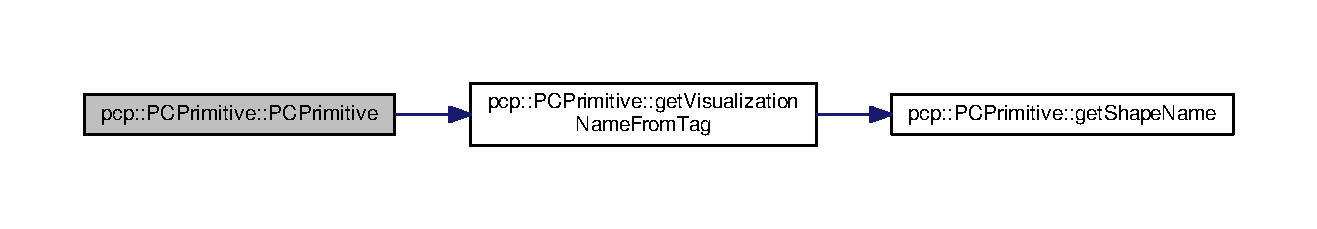
\includegraphics[width=350pt]{classpcp_1_1PCPrimitive_a00c270f938ac1f76c1252422e1f1424f_cgraph}
\end{center}
\end{figure}


\hypertarget{classpcp_1_1PCPrimitive_a3a4da7e50a67144bc1b5b4dfd376b72e}{\index{pcp\-::\-P\-C\-Primitive@{pcp\-::\-P\-C\-Primitive}!$\sim$\-P\-C\-Primitive@{$\sim$\-P\-C\-Primitive}}
\index{$\sim$\-P\-C\-Primitive@{$\sim$\-P\-C\-Primitive}!pcp::PCPrimitive@{pcp\-::\-P\-C\-Primitive}}
\subsubsection[{$\sim$\-P\-C\-Primitive}]{\setlength{\rightskip}{0pt plus 5cm}pcp\-::\-P\-C\-Primitive\-::$\sim$\-P\-C\-Primitive (
\begin{DoxyParamCaption}
{}
\end{DoxyParamCaption}
)\hspace{0.3cm}{\ttfamily [virtual]}}}\label{classpcp_1_1PCPrimitive_a3a4da7e50a67144bc1b5b4dfd376b72e}


Definition at line 26 of file P\-C\-Primitive.\-cpp.



\subsection{Member Function Documentation}
\hypertarget{classpcp_1_1PCPrimitive_a2d8fe7d2a3a6454cb378bdbbff408cf0}{\index{pcp\-::\-P\-C\-Primitive@{pcp\-::\-P\-C\-Primitive}!copy\-Coefficients@{copy\-Coefficients}}
\index{copy\-Coefficients@{copy\-Coefficients}!pcp::PCPrimitive@{pcp\-::\-P\-C\-Primitive}}
\subsubsection[{copy\-Coefficients}]{\setlength{\rightskip}{0pt plus 5cm}Model\-Coefficients pcp\-::\-P\-C\-Primitive\-::copy\-Coefficients (
\begin{DoxyParamCaption}
\item[{Model\-Coefficients\-::\-Ptr}]{input}
\end{DoxyParamCaption}
)\hspace{0.3cm}{\ttfamily [private]}}}\label{classpcp_1_1PCPrimitive_a2d8fe7d2a3a6454cb378bdbbff408cf0}


Definition at line 64 of file P\-C\-Primitive.\-cpp.

\hypertarget{classpcp_1_1PCPrimitive_ac774df2f9bb393e9a1491da1b0131d4f}{\index{pcp\-::\-P\-C\-Primitive@{pcp\-::\-P\-C\-Primitive}!get\-Primitive\-Cloud@{get\-Primitive\-Cloud}}
\index{get\-Primitive\-Cloud@{get\-Primitive\-Cloud}!pcp::PCPrimitive@{pcp\-::\-P\-C\-Primitive}}
\subsubsection[{get\-Primitive\-Cloud}]{\setlength{\rightskip}{0pt plus 5cm}{\bf P\-C\-L\-Cloud} pcp\-::\-P\-C\-Primitive\-::get\-Primitive\-Cloud (
\begin{DoxyParamCaption}
{}
\end{DoxyParamCaption}
)}}\label{classpcp_1_1PCPrimitive_ac774df2f9bb393e9a1491da1b0131d4f}


Definition at line 88 of file P\-C\-Primitive.\-cpp.



References primitive\-Cloud.

\hypertarget{classpcp_1_1PCPrimitive_aafdd30869b5e09e394d70efebe5eac2a}{\index{pcp\-::\-P\-C\-Primitive@{pcp\-::\-P\-C\-Primitive}!get\-Primitive\-Normal@{get\-Primitive\-Normal}}
\index{get\-Primitive\-Normal@{get\-Primitive\-Normal}!pcp::PCPrimitive@{pcp\-::\-P\-C\-Primitive}}
\subsubsection[{get\-Primitive\-Normal}]{\setlength{\rightskip}{0pt plus 5cm}{\bf P\-C\-L\-Normal} pcp\-::\-P\-C\-Primitive\-::get\-Primitive\-Normal (
\begin{DoxyParamCaption}
{}
\end{DoxyParamCaption}
)}}\label{classpcp_1_1PCPrimitive_aafdd30869b5e09e394d70efebe5eac2a}


Definition at line 91 of file P\-C\-Primitive.\-cpp.



References primitive\-Normals.

\hypertarget{classpcp_1_1PCPrimitive_a1251deb8c39370d0ed5e7d2c7290063f}{\index{pcp\-::\-P\-C\-Primitive@{pcp\-::\-P\-C\-Primitive}!get\-Shape\-Mapidx@{get\-Shape\-Mapidx}}
\index{get\-Shape\-Mapidx@{get\-Shape\-Mapidx}!pcp::PCPrimitive@{pcp\-::\-P\-C\-Primitive}}
\subsubsection[{get\-Shape\-Mapidx}]{\setlength{\rightskip}{0pt plus 5cm}int pcp\-::\-P\-C\-Primitive\-::get\-Shape\-Mapidx (
\begin{DoxyParamCaption}
{}
\end{DoxyParamCaption}
)}}\label{classpcp_1_1PCPrimitive_a1251deb8c39370d0ed5e7d2c7290063f}


Definition at line 82 of file P\-C\-Primitive.\-cpp.



References shape\-Map\-Idx.

\hypertarget{classpcp_1_1PCPrimitive_a9f507218fd4c442d0daa4938e2e71c10}{\index{pcp\-::\-P\-C\-Primitive@{pcp\-::\-P\-C\-Primitive}!get\-Shape\-Name@{get\-Shape\-Name}}
\index{get\-Shape\-Name@{get\-Shape\-Name}!pcp::PCPrimitive@{pcp\-::\-P\-C\-Primitive}}
\subsubsection[{get\-Shape\-Name}]{\setlength{\rightskip}{0pt plus 5cm}string pcp\-::\-P\-C\-Primitive\-::get\-Shape\-Name (
\begin{DoxyParamCaption}
{}
\end{DoxyParamCaption}
)}}\label{classpcp_1_1PCPrimitive_a9f507218fd4c442d0daa4938e2e71c10}


Definition at line 73 of file P\-C\-Primitive.\-cpp.



References shape\-Name.



Referenced by get\-Visualization\-Name\-From\-Tag().

\hypertarget{classpcp_1_1PCPrimitive_ad92a83f976c6aac8125c7c8997633f21}{\index{pcp\-::\-P\-C\-Primitive@{pcp\-::\-P\-C\-Primitive}!get\-Visualization\-Flag@{get\-Visualization\-Flag}}
\index{get\-Visualization\-Flag@{get\-Visualization\-Flag}!pcp::PCPrimitive@{pcp\-::\-P\-C\-Primitive}}
\subsubsection[{get\-Visualization\-Flag}]{\setlength{\rightskip}{0pt plus 5cm}bool pcp\-::\-P\-C\-Primitive\-::get\-Visualization\-Flag (
\begin{DoxyParamCaption}
{}
\end{DoxyParamCaption}
)}}\label{classpcp_1_1PCPrimitive_ad92a83f976c6aac8125c7c8997633f21}


Definition at line 79 of file P\-C\-Primitive.\-cpp.



References visualization\-Flag.

\hypertarget{classpcp_1_1PCPrimitive_ae6a97bc88b8cc7e83476413c73e01aeb}{\index{pcp\-::\-P\-C\-Primitive@{pcp\-::\-P\-C\-Primitive}!get\-Visualization\-Name@{get\-Visualization\-Name}}
\index{get\-Visualization\-Name@{get\-Visualization\-Name}!pcp::PCPrimitive@{pcp\-::\-P\-C\-Primitive}}
\subsubsection[{get\-Visualization\-Name}]{\setlength{\rightskip}{0pt plus 5cm}string pcp\-::\-P\-C\-Primitive\-::get\-Visualization\-Name (
\begin{DoxyParamCaption}
{}
\end{DoxyParamCaption}
)}}\label{classpcp_1_1PCPrimitive_ae6a97bc88b8cc7e83476413c73e01aeb}


Definition at line 76 of file P\-C\-Primitive.\-cpp.



References visualization\-Name.

\hypertarget{classpcp_1_1PCPrimitive_a0764e20850fd7392f657d1cc43e8ec77}{\index{pcp\-::\-P\-C\-Primitive@{pcp\-::\-P\-C\-Primitive}!get\-Visualization\-Name\-From\-Tag@{get\-Visualization\-Name\-From\-Tag}}
\index{get\-Visualization\-Name\-From\-Tag@{get\-Visualization\-Name\-From\-Tag}!pcp::PCPrimitive@{pcp\-::\-P\-C\-Primitive}}
\subsubsection[{get\-Visualization\-Name\-From\-Tag}]{\setlength{\rightskip}{0pt plus 5cm}string pcp\-::\-P\-C\-Primitive\-::get\-Visualization\-Name\-From\-Tag (
\begin{DoxyParamCaption}
\item[{int}]{idx}
\end{DoxyParamCaption}
)\hspace{0.3cm}{\ttfamily [private]}}}\label{classpcp_1_1PCPrimitive_a0764e20850fd7392f657d1cc43e8ec77}


Definition at line 35 of file P\-C\-Primitive.\-cpp.



References D\-E\-F\-A\-U\-L\-T\-\_\-\-V\-I\-S\-U\-A\-L\-I\-Z\-A\-T\-I\-O\-N\-\_\-\-N\-A\-M\-E\-\_\-\-S\-E\-P\-A\-R\-A\-T\-O\-R, and get\-Shape\-Name().



Referenced by P\-C\-Primitive().



Here is the call graph for this function\-:\nopagebreak
\begin{figure}[H]
\begin{center}
\leavevmode
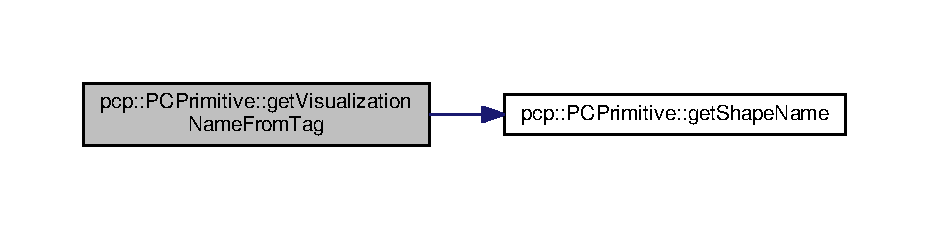
\includegraphics[width=350pt]{classpcp_1_1PCPrimitive_a0764e20850fd7392f657d1cc43e8ec77_cgraph}
\end{center}
\end{figure}




\subsection{Member Data Documentation}
\hypertarget{classpcp_1_1PCPrimitive_ab54a8fb25b750b3808d652f25161ba02}{\index{pcp\-::\-P\-C\-Primitive@{pcp\-::\-P\-C\-Primitive}!D\-E\-F\-A\-U\-L\-T\-\_\-\-S\-H\-A\-P\-E\-\_\-\-N\-A\-M\-E\-\_\-\-C\-L\-U\-S\-T\-E\-R@{D\-E\-F\-A\-U\-L\-T\-\_\-\-S\-H\-A\-P\-E\-\_\-\-N\-A\-M\-E\-\_\-\-C\-L\-U\-S\-T\-E\-R}}
\index{D\-E\-F\-A\-U\-L\-T\-\_\-\-S\-H\-A\-P\-E\-\_\-\-N\-A\-M\-E\-\_\-\-C\-L\-U\-S\-T\-E\-R@{D\-E\-F\-A\-U\-L\-T\-\_\-\-S\-H\-A\-P\-E\-\_\-\-N\-A\-M\-E\-\_\-\-C\-L\-U\-S\-T\-E\-R}!pcp::PCPrimitive@{pcp\-::\-P\-C\-Primitive}}
\subsubsection[{D\-E\-F\-A\-U\-L\-T\-\_\-\-S\-H\-A\-P\-E\-\_\-\-N\-A\-M\-E\-\_\-\-C\-L\-U\-S\-T\-E\-R}]{\setlength{\rightskip}{0pt plus 5cm}const string pcp\-::\-P\-C\-Primitive\-::\-D\-E\-F\-A\-U\-L\-T\-\_\-\-S\-H\-A\-P\-E\-\_\-\-N\-A\-M\-E\-\_\-\-C\-L\-U\-S\-T\-E\-R = \char`\"{}cluster\char`\"{}\hspace{0.3cm}{\ttfamily [static]}}}\label{classpcp_1_1PCPrimitive_ab54a8fb25b750b3808d652f25161ba02}


Definition at line 74 of file P\-C\-Primitive.\-h.

\hypertarget{classpcp_1_1PCPrimitive_a640bb9e84b55d900e6edbaef8b938d6e}{\index{pcp\-::\-P\-C\-Primitive@{pcp\-::\-P\-C\-Primitive}!D\-E\-F\-A\-U\-L\-T\-\_\-\-S\-H\-A\-P\-E\-\_\-\-N\-A\-M\-E\-\_\-\-P\-L\-A\-N\-E@{D\-E\-F\-A\-U\-L\-T\-\_\-\-S\-H\-A\-P\-E\-\_\-\-N\-A\-M\-E\-\_\-\-P\-L\-A\-N\-E}}
\index{D\-E\-F\-A\-U\-L\-T\-\_\-\-S\-H\-A\-P\-E\-\_\-\-N\-A\-M\-E\-\_\-\-P\-L\-A\-N\-E@{D\-E\-F\-A\-U\-L\-T\-\_\-\-S\-H\-A\-P\-E\-\_\-\-N\-A\-M\-E\-\_\-\-P\-L\-A\-N\-E}!pcp::PCPrimitive@{pcp\-::\-P\-C\-Primitive}}
\subsubsection[{D\-E\-F\-A\-U\-L\-T\-\_\-\-S\-H\-A\-P\-E\-\_\-\-N\-A\-M\-E\-\_\-\-P\-L\-A\-N\-E}]{\setlength{\rightskip}{0pt plus 5cm}const string pcp\-::\-P\-C\-Primitive\-::\-D\-E\-F\-A\-U\-L\-T\-\_\-\-S\-H\-A\-P\-E\-\_\-\-N\-A\-M\-E\-\_\-\-P\-L\-A\-N\-E = \char`\"{}plane\char`\"{}\hspace{0.3cm}{\ttfamily [static]}}}\label{classpcp_1_1PCPrimitive_a640bb9e84b55d900e6edbaef8b938d6e}


Definition at line 73 of file P\-C\-Primitive.\-h.

\hypertarget{classpcp_1_1PCPrimitive_a9dc28983a955e1f9b1813a15e4260386}{\index{pcp\-::\-P\-C\-Primitive@{pcp\-::\-P\-C\-Primitive}!D\-E\-F\-A\-U\-L\-T\-\_\-\-V\-I\-S\-U\-A\-L\-I\-Z\-A\-T\-I\-O\-N\-\_\-\-N\-A\-M\-E\-\_\-\-S\-E\-P\-A\-R\-A\-T\-O\-R@{D\-E\-F\-A\-U\-L\-T\-\_\-\-V\-I\-S\-U\-A\-L\-I\-Z\-A\-T\-I\-O\-N\-\_\-\-N\-A\-M\-E\-\_\-\-S\-E\-P\-A\-R\-A\-T\-O\-R}}
\index{D\-E\-F\-A\-U\-L\-T\-\_\-\-V\-I\-S\-U\-A\-L\-I\-Z\-A\-T\-I\-O\-N\-\_\-\-N\-A\-M\-E\-\_\-\-S\-E\-P\-A\-R\-A\-T\-O\-R@{D\-E\-F\-A\-U\-L\-T\-\_\-\-V\-I\-S\-U\-A\-L\-I\-Z\-A\-T\-I\-O\-N\-\_\-\-N\-A\-M\-E\-\_\-\-S\-E\-P\-A\-R\-A\-T\-O\-R}!pcp::PCPrimitive@{pcp\-::\-P\-C\-Primitive}}
\subsubsection[{D\-E\-F\-A\-U\-L\-T\-\_\-\-V\-I\-S\-U\-A\-L\-I\-Z\-A\-T\-I\-O\-N\-\_\-\-N\-A\-M\-E\-\_\-\-S\-E\-P\-A\-R\-A\-T\-O\-R}]{\setlength{\rightskip}{0pt plus 5cm}const string pcp\-::\-P\-C\-Primitive\-::\-D\-E\-F\-A\-U\-L\-T\-\_\-\-V\-I\-S\-U\-A\-L\-I\-Z\-A\-T\-I\-O\-N\-\_\-\-N\-A\-M\-E\-\_\-\-S\-E\-P\-A\-R\-A\-T\-O\-R = \char`\"{}-\/\char`\"{}\hspace{0.3cm}{\ttfamily [static]}}}\label{classpcp_1_1PCPrimitive_a9dc28983a955e1f9b1813a15e4260386}


Definition at line 76 of file P\-C\-Primitive.\-h.



Referenced by get\-Visualization\-Name\-From\-Tag().

\hypertarget{classpcp_1_1PCPrimitive_accdf8a12234519275d4276b6706d4703}{\index{pcp\-::\-P\-C\-Primitive@{pcp\-::\-P\-C\-Primitive}!primitive\-Cloud@{primitive\-Cloud}}
\index{primitive\-Cloud@{primitive\-Cloud}!pcp::PCPrimitive@{pcp\-::\-P\-C\-Primitive}}
\subsubsection[{primitive\-Cloud}]{\setlength{\rightskip}{0pt plus 5cm}{\bf P\-C\-L\-Cloud} pcp\-::\-P\-C\-Primitive\-::primitive\-Cloud\hspace{0.3cm}{\ttfamily [private]}}}\label{classpcp_1_1PCPrimitive_accdf8a12234519275d4276b6706d4703}


Definition at line 37 of file P\-C\-Primitive.\-h.



Referenced by get\-Primitive\-Cloud(), and P\-C\-Primitive().

\hypertarget{classpcp_1_1PCPrimitive_adb0f70b618dddbff203bccd1fa071782}{\index{pcp\-::\-P\-C\-Primitive@{pcp\-::\-P\-C\-Primitive}!primitive\-Coefficients@{primitive\-Coefficients}}
\index{primitive\-Coefficients@{primitive\-Coefficients}!pcp::PCPrimitive@{pcp\-::\-P\-C\-Primitive}}
\subsubsection[{primitive\-Coefficients}]{\setlength{\rightskip}{0pt plus 5cm}Model\-Coefficients pcp\-::\-P\-C\-Primitive\-::primitive\-Coefficients\hspace{0.3cm}{\ttfamily [private]}}}\label{classpcp_1_1PCPrimitive_adb0f70b618dddbff203bccd1fa071782}


Definition at line 39 of file P\-C\-Primitive.\-h.

\hypertarget{classpcp_1_1PCPrimitive_a96359fda0d8c70e3b074d97bde90b282}{\index{pcp\-::\-P\-C\-Primitive@{pcp\-::\-P\-C\-Primitive}!primitive\-Normals@{primitive\-Normals}}
\index{primitive\-Normals@{primitive\-Normals}!pcp::PCPrimitive@{pcp\-::\-P\-C\-Primitive}}
\subsubsection[{primitive\-Normals}]{\setlength{\rightskip}{0pt plus 5cm}{\bf P\-C\-L\-Normal} pcp\-::\-P\-C\-Primitive\-::primitive\-Normals\hspace{0.3cm}{\ttfamily [private]}}}\label{classpcp_1_1PCPrimitive_a96359fda0d8c70e3b074d97bde90b282}


Definition at line 38 of file P\-C\-Primitive.\-h.



Referenced by get\-Primitive\-Normal(), and P\-C\-Primitive().

\hypertarget{classpcp_1_1PCPrimitive_a809c274d155e9b552cf02a0687b7cc11}{\index{pcp\-::\-P\-C\-Primitive@{pcp\-::\-P\-C\-Primitive}!shape\-Map\-Idx@{shape\-Map\-Idx}}
\index{shape\-Map\-Idx@{shape\-Map\-Idx}!pcp::PCPrimitive@{pcp\-::\-P\-C\-Primitive}}
\subsubsection[{shape\-Map\-Idx}]{\setlength{\rightskip}{0pt plus 5cm}int pcp\-::\-P\-C\-Primitive\-::shape\-Map\-Idx\hspace{0.3cm}{\ttfamily [private]}}}\label{classpcp_1_1PCPrimitive_a809c274d155e9b552cf02a0687b7cc11}


Definition at line 34 of file P\-C\-Primitive.\-h.



Referenced by get\-Shape\-Mapidx(), and P\-C\-Primitive().

\hypertarget{classpcp_1_1PCPrimitive_a120d0dd6120b9fe1af74d698d40adb1c}{\index{pcp\-::\-P\-C\-Primitive@{pcp\-::\-P\-C\-Primitive}!shape\-Name@{shape\-Name}}
\index{shape\-Name@{shape\-Name}!pcp::PCPrimitive@{pcp\-::\-P\-C\-Primitive}}
\subsubsection[{shape\-Name}]{\setlength{\rightskip}{0pt plus 5cm}string pcp\-::\-P\-C\-Primitive\-::shape\-Name\hspace{0.3cm}{\ttfamily [private]}}}\label{classpcp_1_1PCPrimitive_a120d0dd6120b9fe1af74d698d40adb1c}


Definition at line 30 of file P\-C\-Primitive.\-h.



Referenced by get\-Shape\-Name(), and P\-C\-Primitive().

\hypertarget{classpcp_1_1PCPrimitive_a44cc3f58388966da71e1b07b52d3081c}{\index{pcp\-::\-P\-C\-Primitive@{pcp\-::\-P\-C\-Primitive}!visualization\-Flag@{visualization\-Flag}}
\index{visualization\-Flag@{visualization\-Flag}!pcp::PCPrimitive@{pcp\-::\-P\-C\-Primitive}}
\subsubsection[{visualization\-Flag}]{\setlength{\rightskip}{0pt plus 5cm}bool pcp\-::\-P\-C\-Primitive\-::visualization\-Flag\hspace{0.3cm}{\ttfamily [private]}}}\label{classpcp_1_1PCPrimitive_a44cc3f58388966da71e1b07b52d3081c}


Definition at line 32 of file P\-C\-Primitive.\-h.



Referenced by get\-Visualization\-Flag(), and P\-C\-Primitive().

\hypertarget{classpcp_1_1PCPrimitive_a8ac9332a85fb342e957959c97012f4d3}{\index{pcp\-::\-P\-C\-Primitive@{pcp\-::\-P\-C\-Primitive}!visualization\-Name@{visualization\-Name}}
\index{visualization\-Name@{visualization\-Name}!pcp::PCPrimitive@{pcp\-::\-P\-C\-Primitive}}
\subsubsection[{visualization\-Name}]{\setlength{\rightskip}{0pt plus 5cm}string pcp\-::\-P\-C\-Primitive\-::visualization\-Name\hspace{0.3cm}{\ttfamily [private]}}}\label{classpcp_1_1PCPrimitive_a8ac9332a85fb342e957959c97012f4d3}


Definition at line 31 of file P\-C\-Primitive.\-h.



Referenced by get\-Visualization\-Name(), and P\-C\-Primitive().



The documentation for this class was generated from the following files\-:\begin{DoxyCompactItemize}
\item 
\hyperlink{PCPrimitive_8h}{P\-C\-Primitive.\-h}\item 
\hyperlink{PCPrimitive_8cpp}{P\-C\-Primitive.\-cpp}\end{DoxyCompactItemize}

\hypertarget{structvector3d}{\section{vector3d Struct Reference}
\label{structvector3d}\index{vector3d@{vector3d}}
}
\subsection*{Public Attributes}
\begin{DoxyCompactItemize}
\item 
float \hyperlink{structvector3d_add24ba608397ce7664f51369fc6a1ba4}{x}
\item 
float \hyperlink{structvector3d_a64dec3fa34e765f42a7c716dbc4559d2}{y}
\item 
float \hyperlink{structvector3d_a4e5e948ffcf14e91ebec29e889ced5be}{z}
\end{DoxyCompactItemize}


\subsection{Detailed Description}


Definition at line 25 of file cone\-Segmentation\-Server.\-cpp.



\subsection{Member Data Documentation}
\hypertarget{structvector3d_add24ba608397ce7664f51369fc6a1ba4}{\index{vector3d@{vector3d}!x@{x}}
\index{x@{x}!vector3d@{vector3d}}
\subsubsection[{x}]{\setlength{\rightskip}{0pt plus 5cm}float vector3d\-::x}}\label{structvector3d_add24ba608397ce7664f51369fc6a1ba4}


Definition at line 26 of file cone\-Segmentation\-Server.\-cpp.



Referenced by get\-Normalize\-Axes\-Direction\-Vector(), get\-Point\-On\-Axes(), get\-Vector\-Between\-Points(), ransac\-Cone\-Detaction(), and ransac\-Cylinder\-Detaction().

\hypertarget{structvector3d_a64dec3fa34e765f42a7c716dbc4559d2}{\index{vector3d@{vector3d}!y@{y}}
\index{y@{y}!vector3d@{vector3d}}
\subsubsection[{y}]{\setlength{\rightskip}{0pt plus 5cm}float vector3d\-::y}}\label{structvector3d_a64dec3fa34e765f42a7c716dbc4559d2}


Definition at line 27 of file cone\-Segmentation\-Server.\-cpp.



Referenced by get\-Normalize\-Axes\-Direction\-Vector(), get\-Point\-On\-Axes(), get\-Vector\-Between\-Points(), ransac\-Cone\-Detaction(), and ransac\-Cylinder\-Detaction().

\hypertarget{structvector3d_a4e5e948ffcf14e91ebec29e889ced5be}{\index{vector3d@{vector3d}!z@{z}}
\index{z@{z}!vector3d@{vector3d}}
\subsubsection[{z}]{\setlength{\rightskip}{0pt plus 5cm}float vector3d\-::z}}\label{structvector3d_a4e5e948ffcf14e91ebec29e889ced5be}


Definition at line 28 of file cone\-Segmentation\-Server.\-cpp.



Referenced by get\-Normalize\-Axes\-Direction\-Vector(), get\-Point\-On\-Axes(), get\-Vector\-Between\-Points(), ransac\-Cone\-Detaction(), and ransac\-Cylinder\-Detaction().



The documentation for this struct was generated from the following files\-:\begin{DoxyCompactItemize}
\item 
\hyperlink{coneSegmentationServer_8cpp}{cone\-Segmentation\-Server.\-cpp}\item 
\hyperlink{cylinderSegmentationServer_8cpp}{cylinder\-Segmentation\-Server.\-cpp}\end{DoxyCompactItemize}

\chapter{File Documentation}
\hypertarget{clusterSegmentationServer_8cpp}{\section{cluster\-Segmentation\-Server.\-cpp File Reference}
\label{clusterSegmentationServer_8cpp}\index{cluster\-Segmentation\-Server.\-cpp@{cluster\-Segmentation\-Server.\-cpp}}
}
{\ttfamily \#include \char`\"{}ros/ros.\-h\char`\"{}}\\*
{\ttfamily \#include $<$iostream$>$}\\*
{\ttfamily \#include \char`\"{}pitt\-\_\-msgs/\-Cluster\-Segmentation.\-h\char`\"{}}\\*
{\ttfamily \#include \char`\"{}pitt\-\_\-msgs/\-Inliers\-Cluster.\-h\char`\"{}}\\*
{\ttfamily \#include $<$pcl\-\_\-ros/point\-\_\-cloud.\-h$>$}\\*
{\ttfamily \#include $<$pcl/segmentation/extract\-\_\-clusters.\-h$>$}\\*
{\ttfamily \#include $<$std\-\_\-msgs/\-String.\-h$>$}\\*
{\ttfamily \#include $<$pcl\-\_\-conversions/pcl\-\_\-conversions.\-h$>$}\\*
{\ttfamily \#include \char`\"{}../\-P\-C\-Static\-Processing/\-P\-C\-Manager.\-h\char`\"{}}\\*
Include dependency graph for cluster\-Segmentation\-Server.\-cpp\-:\nopagebreak
\begin{figure}[H]
\begin{center}
\leavevmode
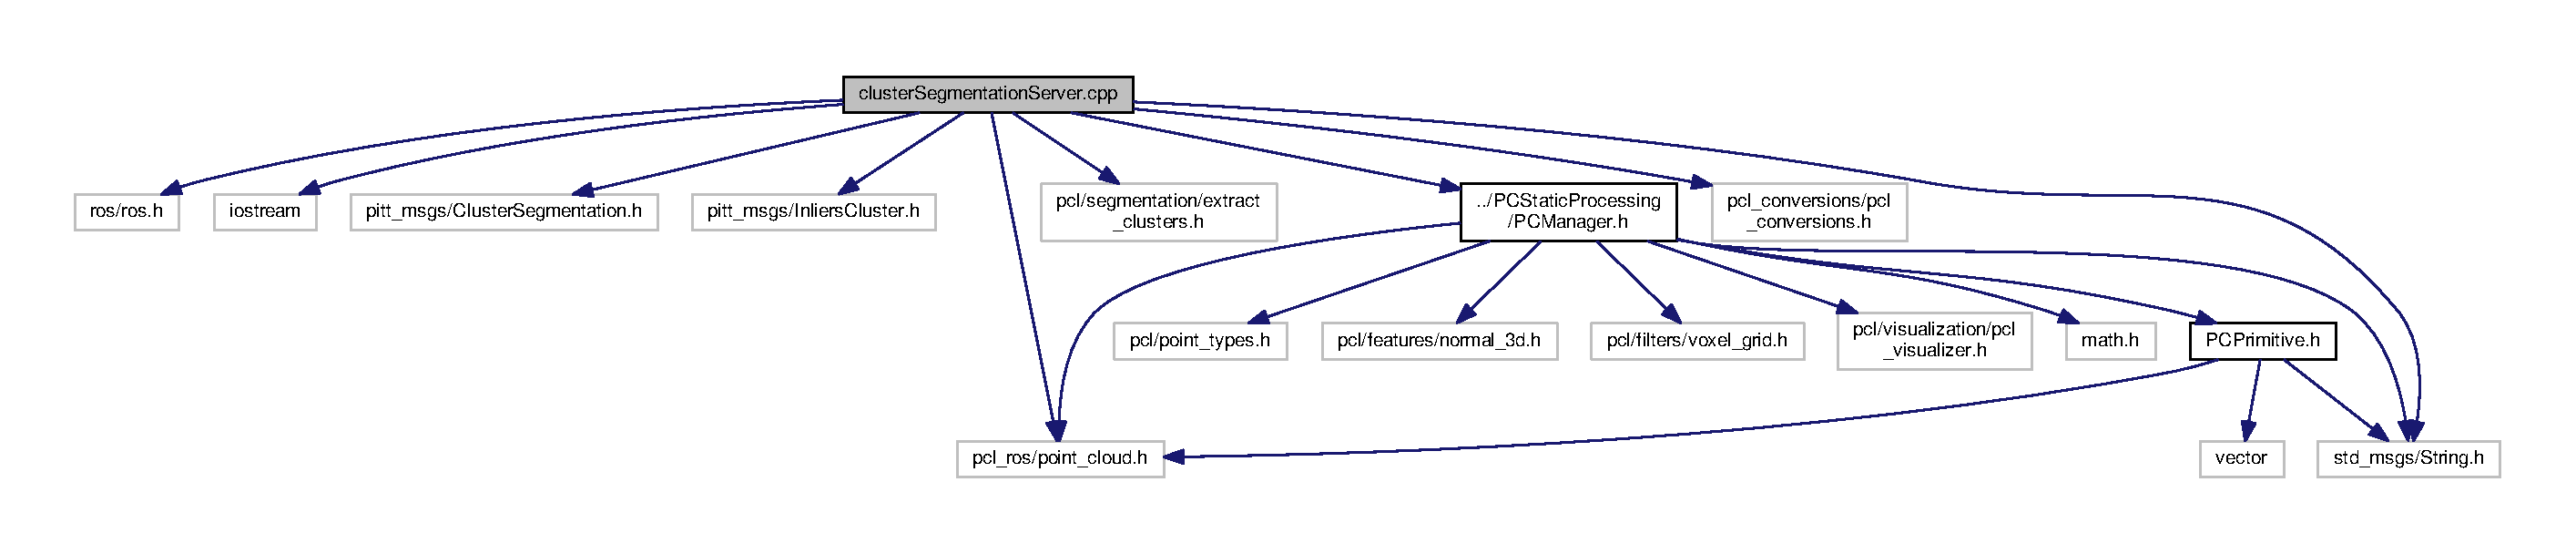
\includegraphics[width=350pt]{clusterSegmentationServer_8cpp__incl}
\end{center}
\end{figure}
\subsection*{Functions}
\begin{DoxyCompactItemize}
\item 
bool \hyperlink{clusterSegmentationServer_8cpp_ab4a01859dbef47b81c5744d85d81a097}{clusterize} (Cluster\-Segmentation\-::\-Request \&req, Cluster\-Segmentation\-::\-Response \&res)
\item 
int \hyperlink{clusterSegmentationServer_8cpp_a3c04138a5bfe5d72780bb7e82a18e627}{main} (int argc, char $\ast$$\ast$argv)
\end{DoxyCompactItemize}
\subsection*{Variables}
\begin{DoxyCompactItemize}
\item 
const float \hyperlink{clusterSegmentationServer_8cpp_a7b24eda7bd663da70a8f6b6c0b4321c9}{T\-O\-L\-L\-E\-R\-A\-N\-C\-E\-\_\-\-D\-E\-F\-A\-U\-L\-T} = 0.\-03f
\item 
const float \hyperlink{clusterSegmentationServer_8cpp_a564e23c724934c557d5aa457f88fb2b2}{M\-I\-N\-\_\-\-C\-L\-U\-S\-T\-E\-R\-\_\-\-R\-A\-T\-E\-\_\-\-D\-E\-F\-A\-U\-L\-T} = 0.\-01f
\item 
const float \hyperlink{clusterSegmentationServer_8cpp_ab08bfd4bf19b043ce4fc7626fe762527}{M\-A\-X\-\_\-\-C\-L\-U\-S\-T\-E\-R\-\_\-\-R\-A\-T\-E\-\_\-\-D\-E\-F\-A\-U\-L\-T} = 0.\-99f
\item 
const float \hyperlink{clusterSegmentationServer_8cpp_a2811162c11f4454598f1e93804117342}{M\-I\-N\-\_\-\-I\-N\-P\-U\-T\-\_\-\-S\-I\-Z\-E\-\_\-\-D\-E\-F\-A\-U\-L\-T} = 30.\-0f
\end{DoxyCompactItemize}


\subsection{Function Documentation}
\hypertarget{clusterSegmentationServer_8cpp_ab4a01859dbef47b81c5744d85d81a097}{\index{cluster\-Segmentation\-Server.\-cpp@{cluster\-Segmentation\-Server.\-cpp}!clusterize@{clusterize}}
\index{clusterize@{clusterize}!clusterSegmentationServer.cpp@{cluster\-Segmentation\-Server.\-cpp}}
\subsubsection[{clusterize}]{\setlength{\rightskip}{0pt plus 5cm}bool clusterize (
\begin{DoxyParamCaption}
\item[{Cluster\-Segmentation\-::\-Request \&}]{req, }
\item[{Cluster\-Segmentation\-::\-Response \&}]{res}
\end{DoxyParamCaption}
)}}\label{clusterSegmentationServer_8cpp_ab4a01859dbef47b81c5744d85d81a097}


Definition at line 33 of file cluster\-Segmentation\-Server.\-cpp.



References pcm\-::\-P\-C\-Manager\-::cloud\-For\-Ros\-Msg(), M\-A\-X\-\_\-\-C\-L\-U\-S\-T\-E\-R\-\_\-\-R\-A\-T\-E\-\_\-\-D\-E\-F\-A\-U\-L\-T, M\-I\-N\-\_\-\-C\-L\-U\-S\-T\-E\-R\-\_\-\-R\-A\-T\-E\-\_\-\-D\-E\-F\-A\-U\-L\-T, M\-I\-N\-\_\-\-I\-N\-P\-U\-T\-\_\-\-S\-I\-Z\-E\-\_\-\-D\-E\-F\-A\-U\-L\-T, T\-O\-L\-L\-E\-R\-A\-N\-C\-E\-\_\-\-D\-E\-F\-A\-U\-L\-T, and pcm\-::tree().



Referenced by main().



Here is the call graph for this function\-:\nopagebreak
\begin{figure}[H]
\begin{center}
\leavevmode
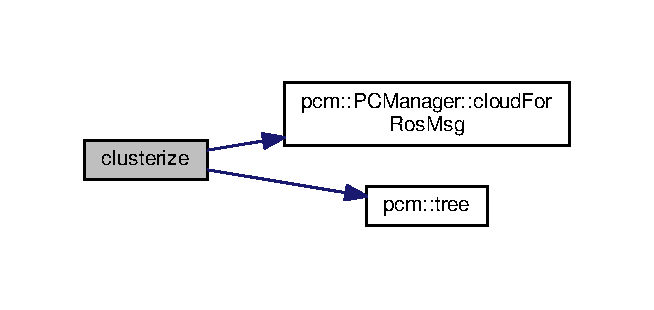
\includegraphics[width=314pt]{clusterSegmentationServer_8cpp_ab4a01859dbef47b81c5744d85d81a097_cgraph}
\end{center}
\end{figure}


\hypertarget{clusterSegmentationServer_8cpp_a3c04138a5bfe5d72780bb7e82a18e627}{\index{cluster\-Segmentation\-Server.\-cpp@{cluster\-Segmentation\-Server.\-cpp}!main@{main}}
\index{main@{main}!clusterSegmentationServer.cpp@{cluster\-Segmentation\-Server.\-cpp}}
\subsubsection[{main}]{\setlength{\rightskip}{0pt plus 5cm}int main (
\begin{DoxyParamCaption}
\item[{int}]{argc, }
\item[{char $\ast$$\ast$}]{argv}
\end{DoxyParamCaption}
)}}\label{clusterSegmentationServer_8cpp_a3c04138a5bfe5d72780bb7e82a18e627}


Definition at line 118 of file cluster\-Segmentation\-Server.\-cpp.



References clusterize().



Here is the call graph for this function\-:\nopagebreak
\begin{figure}[H]
\begin{center}
\leavevmode
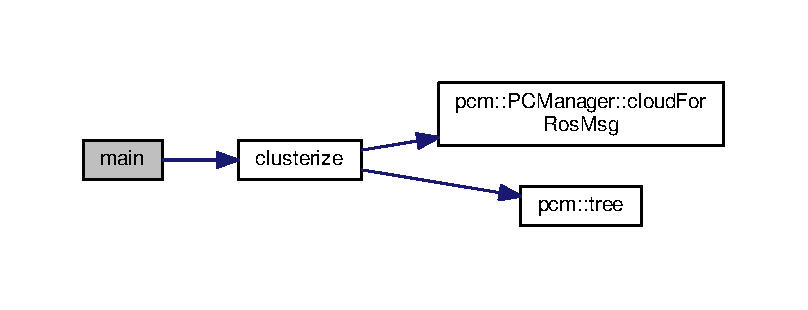
\includegraphics[width=350pt]{clusterSegmentationServer_8cpp_a3c04138a5bfe5d72780bb7e82a18e627_cgraph}
\end{center}
\end{figure}




\subsection{Variable Documentation}
\hypertarget{clusterSegmentationServer_8cpp_ab08bfd4bf19b043ce4fc7626fe762527}{\index{cluster\-Segmentation\-Server.\-cpp@{cluster\-Segmentation\-Server.\-cpp}!M\-A\-X\-\_\-\-C\-L\-U\-S\-T\-E\-R\-\_\-\-R\-A\-T\-E\-\_\-\-D\-E\-F\-A\-U\-L\-T@{M\-A\-X\-\_\-\-C\-L\-U\-S\-T\-E\-R\-\_\-\-R\-A\-T\-E\-\_\-\-D\-E\-F\-A\-U\-L\-T}}
\index{M\-A\-X\-\_\-\-C\-L\-U\-S\-T\-E\-R\-\_\-\-R\-A\-T\-E\-\_\-\-D\-E\-F\-A\-U\-L\-T@{M\-A\-X\-\_\-\-C\-L\-U\-S\-T\-E\-R\-\_\-\-R\-A\-T\-E\-\_\-\-D\-E\-F\-A\-U\-L\-T}!clusterSegmentationServer.cpp@{cluster\-Segmentation\-Server.\-cpp}}
\subsubsection[{M\-A\-X\-\_\-\-C\-L\-U\-S\-T\-E\-R\-\_\-\-R\-A\-T\-E\-\_\-\-D\-E\-F\-A\-U\-L\-T}]{\setlength{\rightskip}{0pt plus 5cm}const float M\-A\-X\-\_\-\-C\-L\-U\-S\-T\-E\-R\-\_\-\-R\-A\-T\-E\-\_\-\-D\-E\-F\-A\-U\-L\-T = 0.\-99f}}\label{clusterSegmentationServer_8cpp_ab08bfd4bf19b043ce4fc7626fe762527}


Definition at line 29 of file cluster\-Segmentation\-Server.\-cpp.



Referenced by clusterize().

\hypertarget{clusterSegmentationServer_8cpp_a564e23c724934c557d5aa457f88fb2b2}{\index{cluster\-Segmentation\-Server.\-cpp@{cluster\-Segmentation\-Server.\-cpp}!M\-I\-N\-\_\-\-C\-L\-U\-S\-T\-E\-R\-\_\-\-R\-A\-T\-E\-\_\-\-D\-E\-F\-A\-U\-L\-T@{M\-I\-N\-\_\-\-C\-L\-U\-S\-T\-E\-R\-\_\-\-R\-A\-T\-E\-\_\-\-D\-E\-F\-A\-U\-L\-T}}
\index{M\-I\-N\-\_\-\-C\-L\-U\-S\-T\-E\-R\-\_\-\-R\-A\-T\-E\-\_\-\-D\-E\-F\-A\-U\-L\-T@{M\-I\-N\-\_\-\-C\-L\-U\-S\-T\-E\-R\-\_\-\-R\-A\-T\-E\-\_\-\-D\-E\-F\-A\-U\-L\-T}!clusterSegmentationServer.cpp@{cluster\-Segmentation\-Server.\-cpp}}
\subsubsection[{M\-I\-N\-\_\-\-C\-L\-U\-S\-T\-E\-R\-\_\-\-R\-A\-T\-E\-\_\-\-D\-E\-F\-A\-U\-L\-T}]{\setlength{\rightskip}{0pt plus 5cm}const float M\-I\-N\-\_\-\-C\-L\-U\-S\-T\-E\-R\-\_\-\-R\-A\-T\-E\-\_\-\-D\-E\-F\-A\-U\-L\-T = 0.\-01f}}\label{clusterSegmentationServer_8cpp_a564e23c724934c557d5aa457f88fb2b2}


Definition at line 28 of file cluster\-Segmentation\-Server.\-cpp.



Referenced by clusterize().

\hypertarget{clusterSegmentationServer_8cpp_a2811162c11f4454598f1e93804117342}{\index{cluster\-Segmentation\-Server.\-cpp@{cluster\-Segmentation\-Server.\-cpp}!M\-I\-N\-\_\-\-I\-N\-P\-U\-T\-\_\-\-S\-I\-Z\-E\-\_\-\-D\-E\-F\-A\-U\-L\-T@{M\-I\-N\-\_\-\-I\-N\-P\-U\-T\-\_\-\-S\-I\-Z\-E\-\_\-\-D\-E\-F\-A\-U\-L\-T}}
\index{M\-I\-N\-\_\-\-I\-N\-P\-U\-T\-\_\-\-S\-I\-Z\-E\-\_\-\-D\-E\-F\-A\-U\-L\-T@{M\-I\-N\-\_\-\-I\-N\-P\-U\-T\-\_\-\-S\-I\-Z\-E\-\_\-\-D\-E\-F\-A\-U\-L\-T}!clusterSegmentationServer.cpp@{cluster\-Segmentation\-Server.\-cpp}}
\subsubsection[{M\-I\-N\-\_\-\-I\-N\-P\-U\-T\-\_\-\-S\-I\-Z\-E\-\_\-\-D\-E\-F\-A\-U\-L\-T}]{\setlength{\rightskip}{0pt plus 5cm}const float M\-I\-N\-\_\-\-I\-N\-P\-U\-T\-\_\-\-S\-I\-Z\-E\-\_\-\-D\-E\-F\-A\-U\-L\-T = 30.\-0f}}\label{clusterSegmentationServer_8cpp_a2811162c11f4454598f1e93804117342}


Definition at line 30 of file cluster\-Segmentation\-Server.\-cpp.



Referenced by clusterize().

\hypertarget{clusterSegmentationServer_8cpp_a7b24eda7bd663da70a8f6b6c0b4321c9}{\index{cluster\-Segmentation\-Server.\-cpp@{cluster\-Segmentation\-Server.\-cpp}!T\-O\-L\-L\-E\-R\-A\-N\-C\-E\-\_\-\-D\-E\-F\-A\-U\-L\-T@{T\-O\-L\-L\-E\-R\-A\-N\-C\-E\-\_\-\-D\-E\-F\-A\-U\-L\-T}}
\index{T\-O\-L\-L\-E\-R\-A\-N\-C\-E\-\_\-\-D\-E\-F\-A\-U\-L\-T@{T\-O\-L\-L\-E\-R\-A\-N\-C\-E\-\_\-\-D\-E\-F\-A\-U\-L\-T}!clusterSegmentationServer.cpp@{cluster\-Segmentation\-Server.\-cpp}}
\subsubsection[{T\-O\-L\-L\-E\-R\-A\-N\-C\-E\-\_\-\-D\-E\-F\-A\-U\-L\-T}]{\setlength{\rightskip}{0pt plus 5cm}const float T\-O\-L\-L\-E\-R\-A\-N\-C\-E\-\_\-\-D\-E\-F\-A\-U\-L\-T = 0.\-03f}}\label{clusterSegmentationServer_8cpp_a7b24eda7bd663da70a8f6b6c0b4321c9}


Definition at line 27 of file cluster\-Segmentation\-Server.\-cpp.



Referenced by clusterize().


\hypertarget{coneSegmentationServer_8cpp}{\section{cone\-Segmentation\-Server.\-cpp File Reference}
\label{coneSegmentationServer_8cpp}\index{cone\-Segmentation\-Server.\-cpp@{cone\-Segmentation\-Server.\-cpp}}
}
{\ttfamily \#include \char`\"{}ros/ros.\-h\char`\"{}}\\*
{\ttfamily \#include $<$pcl\-\_\-ros/point\-\_\-cloud.\-h$>$}\\*
{\ttfamily \#include $<$pcl/segmentation/sac\-\_\-segmentation.\-h$>$}\\*
{\ttfamily \#include \char`\"{}../\-P\-C\-Static\-Processing/\-P\-C\-Manager.\-h\char`\"{}}\\*
{\ttfamily \#include \char`\"{}pitt\-\_\-msgs/\-Primitive\-Segmentation.\-h\char`\"{}}\\*
Include dependency graph for cone\-Segmentation\-Server.\-cpp\-:\nopagebreak
\begin{figure}[H]
\begin{center}
\leavevmode
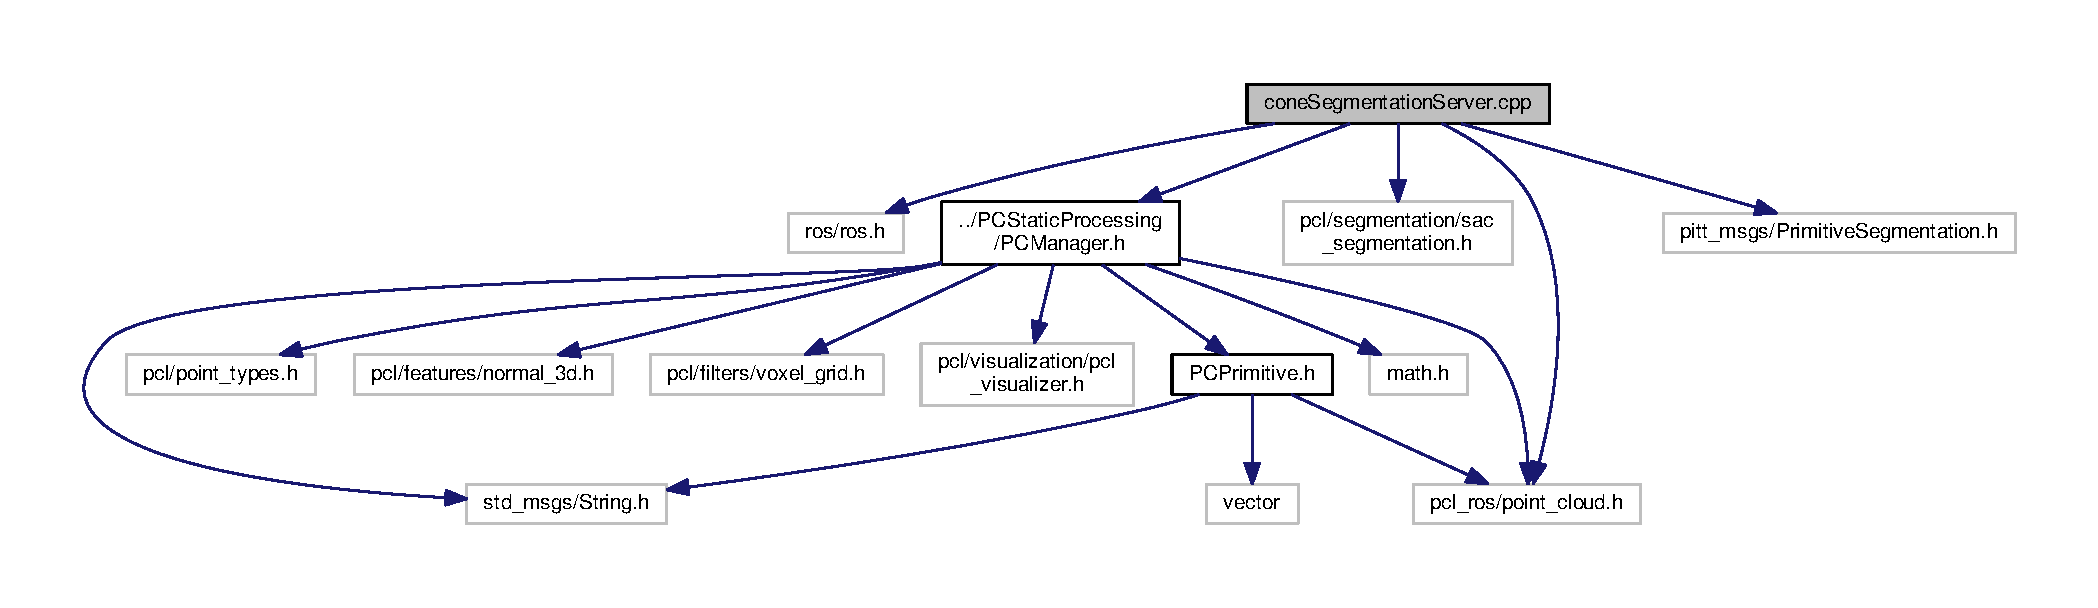
\includegraphics[width=350pt]{coneSegmentationServer_8cpp__incl}
\end{center}
\end{figure}
\subsection*{Classes}
\begin{DoxyCompactItemize}
\item 
struct \hyperlink{structvector3d}{vector3d}
\end{DoxyCompactItemize}
\subsection*{Functions}
\begin{DoxyCompactItemize}
\item 
\hyperlink{structvector3d}{vector3d} \hyperlink{coneSegmentationServer_8cpp_a18fcf7fa2e84ef1176c2ca1abed744cf}{get\-Normalize\-Axes\-Direction\-Vector} (Model\-Coefficients\-::\-Ptr coefficients)
\item 
\hyperlink{structvector3d}{vector3d} \hyperlink{coneSegmentationServer_8cpp_a255909b8e4ba570eea6756718bf79df1}{get\-Point\-On\-Axes} (Model\-Coefficients\-::\-Ptr coefficients, \hyperlink{structvector3d}{vector3d} direction, float t)
\item 
\hyperlink{structvector3d}{vector3d} \hyperlink{coneSegmentationServer_8cpp_a00c9eb33d55847838be7bf32c23d1893}{get\-Vector\-Between\-Points} (\hyperlink{structvector3d}{vector3d} p1, \hyperlink{structvector3d}{vector3d} p2)
\item 
bool \hyperlink{coneSegmentationServer_8cpp_a546c9eceb49309d94085dada4aae1755}{ransac\-Cone\-Detaction} (Primitive\-Segmentation\-::\-Request \&req, Primitive\-Segmentation\-::\-Response \&res)
\item 
int \hyperlink{coneSegmentationServer_8cpp_a3c04138a5bfe5d72780bb7e82a18e627}{main} (int argc, char $\ast$$\ast$argv)
\end{DoxyCompactItemize}
\subsection*{Variables}
\begin{DoxyCompactItemize}
\item 
const float \hyperlink{coneSegmentationServer_8cpp_a6a60b5e5200860d75f403dcf05dde9ef}{N\-O\-R\-M\-A\-L\-\_\-\-D\-I\-S\-T\-A\-N\-C\-E\-\_\-\-W\-E\-I\-G\-H\-T\-\_\-\-D\-E\-F\-A\-U\-L\-T} = 0.\-0006f
\item 
const float \hyperlink{coneSegmentationServer_8cpp_a73e7be3a150e91558f7c5e69c03dd6e6}{D\-I\-S\-T\-A\-N\-C\-E\-\_\-\-T\-H\-R\-E\-S\-H\-O\-L\-D\-\_\-\-D\-E\-F\-A\-U\-L\-T} = 0.\-0055f
\item 
const int \hyperlink{coneSegmentationServer_8cpp_aeb805bfa6116e2c314b0ebc3c73c6504}{M\-A\-X\-\_\-\-I\-T\-E\-R\-A\-T\-I\-O\-N\-\_\-\-D\-E\-F\-A\-U\-L\-T} = 1000
\item 
const float \hyperlink{coneSegmentationServer_8cpp_aa84d6979d2a503e253f54c3e069abaf5}{M\-I\-N\-\_\-\-R\-A\-D\-I\-U\-S\-\_\-\-L\-I\-M\-I\-T} = 0.\-001
\item 
const float \hyperlink{coneSegmentationServer_8cpp_abcdbdc04946f1566041df18c6c892f0f}{M\-A\-X\-\_\-\-R\-A\-D\-I\-U\-S\-\_\-\-L\-I\-M\-I\-T} = 0.\-500
\item 
const float \hyperlink{coneSegmentationServer_8cpp_a32a067fb9ad7cc8e19b52018946d374d}{E\-P\-S\-\_\-\-A\-N\-G\-L\-E} = 0.\-4f
\item 
const float \hyperlink{coneSegmentationServer_8cpp_ae71c4fb043a78285d76d4dcbd7231e70}{M\-I\-N\-\_\-\-O\-P\-E\-N\-I\-N\-G\-\_\-\-A\-N\-G\-L\-E} = 10.\-0f
\item 
const float \hyperlink{coneSegmentationServer_8cpp_afaeeefd6f578a58f8e14040f6176c394}{M\-A\-X\-\_\-\-O\-P\-E\-N\-I\-N\-G\-\_\-\-A\-N\-G\-L\-E} = 170.\-0f
\item 
const bool \hyperlink{coneSegmentationServer_8cpp_a20f88026cd9df482d817a3868c20fe43}{V\-I\-S\-U\-A\-L\-I\-Z\-E\-\_\-\-R\-E\-S\-U\-L\-T} = false
\item 
boost\-::shared\-\_\-ptr\\*
$<$ \hyperlink{PCManager_8h_a38c805dbc7ad6f06109b85c8e540817a}{visualization\-::\-P\-C\-L\-Visualizer} $>$ \hyperlink{coneSegmentationServer_8cpp_a6c2d87234fca8dcca11f888098558986}{vis}
\end{DoxyCompactItemize}


\subsection{Function Documentation}
\hypertarget{coneSegmentationServer_8cpp_a18fcf7fa2e84ef1176c2ca1abed744cf}{\index{cone\-Segmentation\-Server.\-cpp@{cone\-Segmentation\-Server.\-cpp}!get\-Normalize\-Axes\-Direction\-Vector@{get\-Normalize\-Axes\-Direction\-Vector}}
\index{get\-Normalize\-Axes\-Direction\-Vector@{get\-Normalize\-Axes\-Direction\-Vector}!coneSegmentationServer.cpp@{cone\-Segmentation\-Server.\-cpp}}
\subsubsection[{get\-Normalize\-Axes\-Direction\-Vector}]{\setlength{\rightskip}{0pt plus 5cm}{\bf vector3d} get\-Normalize\-Axes\-Direction\-Vector (
\begin{DoxyParamCaption}
\item[{Model\-Coefficients\-::\-Ptr}]{coefficients}
\end{DoxyParamCaption}
)}}\label{coneSegmentationServer_8cpp_a18fcf7fa2e84ef1176c2ca1abed744cf}


Definition at line 36 of file cone\-Segmentation\-Server.\-cpp.



References vector3d\-::x, vector3d\-::y, and vector3d\-::z.



Referenced by ransac\-Cone\-Detaction().

\hypertarget{coneSegmentationServer_8cpp_a255909b8e4ba570eea6756718bf79df1}{\index{cone\-Segmentation\-Server.\-cpp@{cone\-Segmentation\-Server.\-cpp}!get\-Point\-On\-Axes@{get\-Point\-On\-Axes}}
\index{get\-Point\-On\-Axes@{get\-Point\-On\-Axes}!coneSegmentationServer.cpp@{cone\-Segmentation\-Server.\-cpp}}
\subsubsection[{get\-Point\-On\-Axes}]{\setlength{\rightskip}{0pt plus 5cm}{\bf vector3d} get\-Point\-On\-Axes (
\begin{DoxyParamCaption}
\item[{Model\-Coefficients\-::\-Ptr}]{coefficients, }
\item[{{\bf vector3d}}]{direction, }
\item[{float}]{t}
\end{DoxyParamCaption}
)}}\label{coneSegmentationServer_8cpp_a255909b8e4ba570eea6756718bf79df1}


Definition at line 47 of file cone\-Segmentation\-Server.\-cpp.



References vector3d\-::x, vector3d\-::y, and vector3d\-::z.



Referenced by ransac\-Cone\-Detaction().

\hypertarget{coneSegmentationServer_8cpp_a00c9eb33d55847838be7bf32c23d1893}{\index{cone\-Segmentation\-Server.\-cpp@{cone\-Segmentation\-Server.\-cpp}!get\-Vector\-Between\-Points@{get\-Vector\-Between\-Points}}
\index{get\-Vector\-Between\-Points@{get\-Vector\-Between\-Points}!coneSegmentationServer.cpp@{cone\-Segmentation\-Server.\-cpp}}
\subsubsection[{get\-Vector\-Between\-Points}]{\setlength{\rightskip}{0pt plus 5cm}{\bf vector3d} get\-Vector\-Between\-Points (
\begin{DoxyParamCaption}
\item[{{\bf vector3d}}]{p1, }
\item[{{\bf vector3d}}]{p2}
\end{DoxyParamCaption}
)}}\label{coneSegmentationServer_8cpp_a00c9eb33d55847838be7bf32c23d1893}


Definition at line 56 of file cone\-Segmentation\-Server.\-cpp.



References vector3d\-::x, vector3d\-::y, and vector3d\-::z.



Referenced by ransac\-Cone\-Detaction().

\hypertarget{coneSegmentationServer_8cpp_a3c04138a5bfe5d72780bb7e82a18e627}{\index{cone\-Segmentation\-Server.\-cpp@{cone\-Segmentation\-Server.\-cpp}!main@{main}}
\index{main@{main}!coneSegmentationServer.cpp@{cone\-Segmentation\-Server.\-cpp}}
\subsubsection[{main}]{\setlength{\rightskip}{0pt plus 5cm}int main (
\begin{DoxyParamCaption}
\item[{int}]{argc, }
\item[{char $\ast$$\ast$}]{argv}
\end{DoxyParamCaption}
)}}\label{coneSegmentationServer_8cpp_a3c04138a5bfe5d72780bb7e82a18e627}


Definition at line 217 of file cone\-Segmentation\-Server.\-cpp.



References pcm\-::\-P\-C\-Manager\-::create\-Visor(), pcm\-::\-P\-C\-Manager\-::\-R\-A\-N\-S\-A\-C\-\_\-\-C\-O\-N\-E\-\_\-\-F\-I\-L\-T\-E\-R\-\_\-\-S\-E\-R\-V\-I\-C\-E\-\_\-\-N\-A\-M\-E, ransac\-Cone\-Detaction(), vis, and V\-I\-S\-U\-A\-L\-I\-Z\-E\-\_\-\-R\-E\-S\-U\-L\-T.



Here is the call graph for this function\-:\nopagebreak
\begin{figure}[H]
\begin{center}
\leavevmode
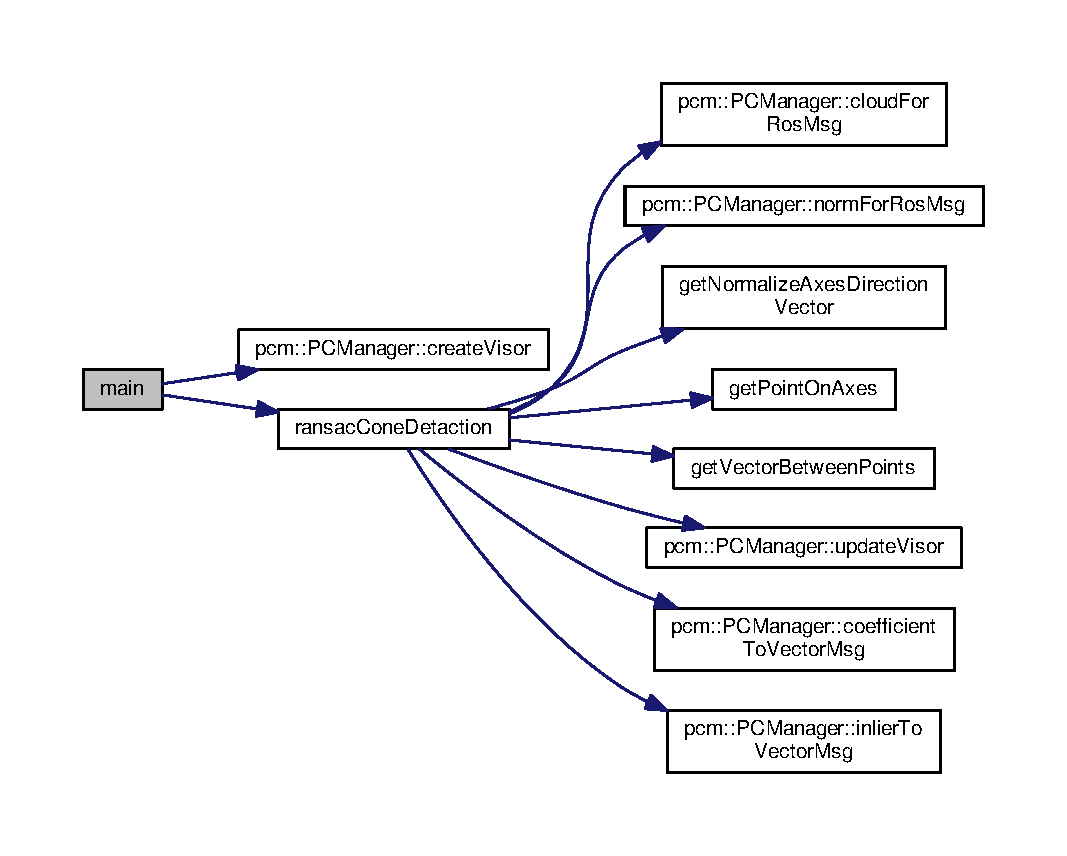
\includegraphics[width=350pt]{coneSegmentationServer_8cpp_a3c04138a5bfe5d72780bb7e82a18e627_cgraph}
\end{center}
\end{figure}


\hypertarget{coneSegmentationServer_8cpp_a546c9eceb49309d94085dada4aae1755}{\index{cone\-Segmentation\-Server.\-cpp@{cone\-Segmentation\-Server.\-cpp}!ransac\-Cone\-Detaction@{ransac\-Cone\-Detaction}}
\index{ransac\-Cone\-Detaction@{ransac\-Cone\-Detaction}!coneSegmentationServer.cpp@{cone\-Segmentation\-Server.\-cpp}}
\subsubsection[{ransac\-Cone\-Detaction}]{\setlength{\rightskip}{0pt plus 5cm}bool ransac\-Cone\-Detaction (
\begin{DoxyParamCaption}
\item[{Primitive\-Segmentation\-::\-Request \&}]{req, }
\item[{Primitive\-Segmentation\-::\-Response \&}]{res}
\end{DoxyParamCaption}
)}}\label{coneSegmentationServer_8cpp_a546c9eceb49309d94085dada4aae1755}


Definition at line 65 of file cone\-Segmentation\-Server.\-cpp.



References pcm\-::\-P\-C\-Manager\-::cloud\-For\-Ros\-Msg(), pcm\-::\-P\-C\-Manager\-::coefficient\-To\-Vector\-Msg(), D\-I\-S\-T\-A\-N\-C\-E\-\_\-\-T\-H\-R\-E\-S\-H\-O\-L\-D\-\_\-\-D\-E\-F\-A\-U\-L\-T, E\-P\-S\-\_\-\-A\-N\-G\-L\-E, get\-Normalize\-Axes\-Direction\-Vector(), get\-Point\-On\-Axes(), get\-Vector\-Between\-Points(), pcm\-::\-P\-C\-Manager\-::inlier\-To\-Vector\-Msg(), M\-A\-X\-\_\-\-I\-T\-E\-R\-A\-T\-I\-O\-N\-\_\-\-D\-E\-F\-A\-U\-L\-T, M\-A\-X\-\_\-\-O\-P\-E\-N\-I\-N\-G\-\_\-\-A\-N\-G\-L\-E, M\-A\-X\-\_\-\-R\-A\-D\-I\-U\-S\-\_\-\-L\-I\-M\-I\-T, M\-I\-N\-\_\-\-O\-P\-E\-N\-I\-N\-G\-\_\-\-A\-N\-G\-L\-E, M\-I\-N\-\_\-\-R\-A\-D\-I\-U\-S\-\_\-\-L\-I\-M\-I\-T, N\-O\-R\-M\-A\-L\-\_\-\-D\-I\-S\-T\-A\-N\-C\-E\-\_\-\-W\-E\-I\-G\-H\-T\-\_\-\-D\-E\-F\-A\-U\-L\-T, pcm\-::\-P\-C\-Manager\-::norm\-For\-Ros\-Msg(), seg, pcm\-::\-P\-C\-Manager\-::update\-Visor(), vis, V\-I\-S\-U\-A\-L\-I\-Z\-E\-\_\-\-R\-E\-S\-U\-L\-T, vector3d\-::x, vector3d\-::y, and vector3d\-::z.



Referenced by main().



Here is the call graph for this function\-:\nopagebreak
\begin{figure}[H]
\begin{center}
\leavevmode
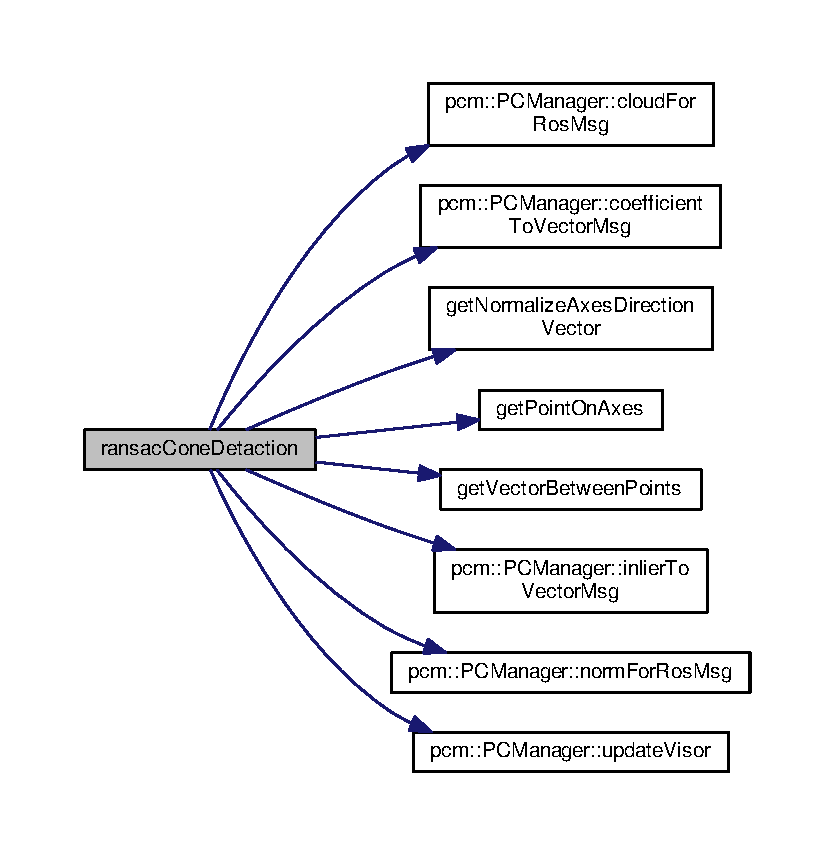
\includegraphics[width=350pt]{coneSegmentationServer_8cpp_a546c9eceb49309d94085dada4aae1755_cgraph}
\end{center}
\end{figure}




\subsection{Variable Documentation}
\hypertarget{coneSegmentationServer_8cpp_a73e7be3a150e91558f7c5e69c03dd6e6}{\index{cone\-Segmentation\-Server.\-cpp@{cone\-Segmentation\-Server.\-cpp}!D\-I\-S\-T\-A\-N\-C\-E\-\_\-\-T\-H\-R\-E\-S\-H\-O\-L\-D\-\_\-\-D\-E\-F\-A\-U\-L\-T@{D\-I\-S\-T\-A\-N\-C\-E\-\_\-\-T\-H\-R\-E\-S\-H\-O\-L\-D\-\_\-\-D\-E\-F\-A\-U\-L\-T}}
\index{D\-I\-S\-T\-A\-N\-C\-E\-\_\-\-T\-H\-R\-E\-S\-H\-O\-L\-D\-\_\-\-D\-E\-F\-A\-U\-L\-T@{D\-I\-S\-T\-A\-N\-C\-E\-\_\-\-T\-H\-R\-E\-S\-H\-O\-L\-D\-\_\-\-D\-E\-F\-A\-U\-L\-T}!coneSegmentationServer.cpp@{cone\-Segmentation\-Server.\-cpp}}
\subsubsection[{D\-I\-S\-T\-A\-N\-C\-E\-\_\-\-T\-H\-R\-E\-S\-H\-O\-L\-D\-\_\-\-D\-E\-F\-A\-U\-L\-T}]{\setlength{\rightskip}{0pt plus 5cm}const float D\-I\-S\-T\-A\-N\-C\-E\-\_\-\-T\-H\-R\-E\-S\-H\-O\-L\-D\-\_\-\-D\-E\-F\-A\-U\-L\-T = 0.\-0055f}}\label{coneSegmentationServer_8cpp_a73e7be3a150e91558f7c5e69c03dd6e6}


Definition at line 16 of file cone\-Segmentation\-Server.\-cpp.



Referenced by ransac\-Cone\-Detaction().

\hypertarget{coneSegmentationServer_8cpp_a32a067fb9ad7cc8e19b52018946d374d}{\index{cone\-Segmentation\-Server.\-cpp@{cone\-Segmentation\-Server.\-cpp}!E\-P\-S\-\_\-\-A\-N\-G\-L\-E@{E\-P\-S\-\_\-\-A\-N\-G\-L\-E}}
\index{E\-P\-S\-\_\-\-A\-N\-G\-L\-E@{E\-P\-S\-\_\-\-A\-N\-G\-L\-E}!coneSegmentationServer.cpp@{cone\-Segmentation\-Server.\-cpp}}
\subsubsection[{E\-P\-S\-\_\-\-A\-N\-G\-L\-E}]{\setlength{\rightskip}{0pt plus 5cm}const float E\-P\-S\-\_\-\-A\-N\-G\-L\-E = 0.\-4f}}\label{coneSegmentationServer_8cpp_a32a067fb9ad7cc8e19b52018946d374d}


Definition at line 20 of file cone\-Segmentation\-Server.\-cpp.



Referenced by ransac\-Cone\-Detaction().

\hypertarget{coneSegmentationServer_8cpp_aeb805bfa6116e2c314b0ebc3c73c6504}{\index{cone\-Segmentation\-Server.\-cpp@{cone\-Segmentation\-Server.\-cpp}!M\-A\-X\-\_\-\-I\-T\-E\-R\-A\-T\-I\-O\-N\-\_\-\-D\-E\-F\-A\-U\-L\-T@{M\-A\-X\-\_\-\-I\-T\-E\-R\-A\-T\-I\-O\-N\-\_\-\-D\-E\-F\-A\-U\-L\-T}}
\index{M\-A\-X\-\_\-\-I\-T\-E\-R\-A\-T\-I\-O\-N\-\_\-\-D\-E\-F\-A\-U\-L\-T@{M\-A\-X\-\_\-\-I\-T\-E\-R\-A\-T\-I\-O\-N\-\_\-\-D\-E\-F\-A\-U\-L\-T}!coneSegmentationServer.cpp@{cone\-Segmentation\-Server.\-cpp}}
\subsubsection[{M\-A\-X\-\_\-\-I\-T\-E\-R\-A\-T\-I\-O\-N\-\_\-\-D\-E\-F\-A\-U\-L\-T}]{\setlength{\rightskip}{0pt plus 5cm}const int M\-A\-X\-\_\-\-I\-T\-E\-R\-A\-T\-I\-O\-N\-\_\-\-D\-E\-F\-A\-U\-L\-T = 1000}}\label{coneSegmentationServer_8cpp_aeb805bfa6116e2c314b0ebc3c73c6504}


Definition at line 17 of file cone\-Segmentation\-Server.\-cpp.



Referenced by ransac\-Cone\-Detaction().

\hypertarget{coneSegmentationServer_8cpp_afaeeefd6f578a58f8e14040f6176c394}{\index{cone\-Segmentation\-Server.\-cpp@{cone\-Segmentation\-Server.\-cpp}!M\-A\-X\-\_\-\-O\-P\-E\-N\-I\-N\-G\-\_\-\-A\-N\-G\-L\-E@{M\-A\-X\-\_\-\-O\-P\-E\-N\-I\-N\-G\-\_\-\-A\-N\-G\-L\-E}}
\index{M\-A\-X\-\_\-\-O\-P\-E\-N\-I\-N\-G\-\_\-\-A\-N\-G\-L\-E@{M\-A\-X\-\_\-\-O\-P\-E\-N\-I\-N\-G\-\_\-\-A\-N\-G\-L\-E}!coneSegmentationServer.cpp@{cone\-Segmentation\-Server.\-cpp}}
\subsubsection[{M\-A\-X\-\_\-\-O\-P\-E\-N\-I\-N\-G\-\_\-\-A\-N\-G\-L\-E}]{\setlength{\rightskip}{0pt plus 5cm}const float M\-A\-X\-\_\-\-O\-P\-E\-N\-I\-N\-G\-\_\-\-A\-N\-G\-L\-E = 170.\-0f}}\label{coneSegmentationServer_8cpp_afaeeefd6f578a58f8e14040f6176c394}


Definition at line 22 of file cone\-Segmentation\-Server.\-cpp.



Referenced by ransac\-Cone\-Detaction().

\hypertarget{coneSegmentationServer_8cpp_abcdbdc04946f1566041df18c6c892f0f}{\index{cone\-Segmentation\-Server.\-cpp@{cone\-Segmentation\-Server.\-cpp}!M\-A\-X\-\_\-\-R\-A\-D\-I\-U\-S\-\_\-\-L\-I\-M\-I\-T@{M\-A\-X\-\_\-\-R\-A\-D\-I\-U\-S\-\_\-\-L\-I\-M\-I\-T}}
\index{M\-A\-X\-\_\-\-R\-A\-D\-I\-U\-S\-\_\-\-L\-I\-M\-I\-T@{M\-A\-X\-\_\-\-R\-A\-D\-I\-U\-S\-\_\-\-L\-I\-M\-I\-T}!coneSegmentationServer.cpp@{cone\-Segmentation\-Server.\-cpp}}
\subsubsection[{M\-A\-X\-\_\-\-R\-A\-D\-I\-U\-S\-\_\-\-L\-I\-M\-I\-T}]{\setlength{\rightskip}{0pt plus 5cm}const float M\-A\-X\-\_\-\-R\-A\-D\-I\-U\-S\-\_\-\-L\-I\-M\-I\-T = 0.\-500}}\label{coneSegmentationServer_8cpp_abcdbdc04946f1566041df18c6c892f0f}


Definition at line 19 of file cone\-Segmentation\-Server.\-cpp.



Referenced by ransac\-Cone\-Detaction().

\hypertarget{coneSegmentationServer_8cpp_ae71c4fb043a78285d76d4dcbd7231e70}{\index{cone\-Segmentation\-Server.\-cpp@{cone\-Segmentation\-Server.\-cpp}!M\-I\-N\-\_\-\-O\-P\-E\-N\-I\-N\-G\-\_\-\-A\-N\-G\-L\-E@{M\-I\-N\-\_\-\-O\-P\-E\-N\-I\-N\-G\-\_\-\-A\-N\-G\-L\-E}}
\index{M\-I\-N\-\_\-\-O\-P\-E\-N\-I\-N\-G\-\_\-\-A\-N\-G\-L\-E@{M\-I\-N\-\_\-\-O\-P\-E\-N\-I\-N\-G\-\_\-\-A\-N\-G\-L\-E}!coneSegmentationServer.cpp@{cone\-Segmentation\-Server.\-cpp}}
\subsubsection[{M\-I\-N\-\_\-\-O\-P\-E\-N\-I\-N\-G\-\_\-\-A\-N\-G\-L\-E}]{\setlength{\rightskip}{0pt plus 5cm}const float M\-I\-N\-\_\-\-O\-P\-E\-N\-I\-N\-G\-\_\-\-A\-N\-G\-L\-E = 10.\-0f}}\label{coneSegmentationServer_8cpp_ae71c4fb043a78285d76d4dcbd7231e70}


Definition at line 21 of file cone\-Segmentation\-Server.\-cpp.



Referenced by ransac\-Cone\-Detaction().

\hypertarget{coneSegmentationServer_8cpp_aa84d6979d2a503e253f54c3e069abaf5}{\index{cone\-Segmentation\-Server.\-cpp@{cone\-Segmentation\-Server.\-cpp}!M\-I\-N\-\_\-\-R\-A\-D\-I\-U\-S\-\_\-\-L\-I\-M\-I\-T@{M\-I\-N\-\_\-\-R\-A\-D\-I\-U\-S\-\_\-\-L\-I\-M\-I\-T}}
\index{M\-I\-N\-\_\-\-R\-A\-D\-I\-U\-S\-\_\-\-L\-I\-M\-I\-T@{M\-I\-N\-\_\-\-R\-A\-D\-I\-U\-S\-\_\-\-L\-I\-M\-I\-T}!coneSegmentationServer.cpp@{cone\-Segmentation\-Server.\-cpp}}
\subsubsection[{M\-I\-N\-\_\-\-R\-A\-D\-I\-U\-S\-\_\-\-L\-I\-M\-I\-T}]{\setlength{\rightskip}{0pt plus 5cm}const float M\-I\-N\-\_\-\-R\-A\-D\-I\-U\-S\-\_\-\-L\-I\-M\-I\-T = 0.\-001}}\label{coneSegmentationServer_8cpp_aa84d6979d2a503e253f54c3e069abaf5}


Definition at line 18 of file cone\-Segmentation\-Server.\-cpp.



Referenced by ransac\-Cone\-Detaction().

\hypertarget{coneSegmentationServer_8cpp_a6a60b5e5200860d75f403dcf05dde9ef}{\index{cone\-Segmentation\-Server.\-cpp@{cone\-Segmentation\-Server.\-cpp}!N\-O\-R\-M\-A\-L\-\_\-\-D\-I\-S\-T\-A\-N\-C\-E\-\_\-\-W\-E\-I\-G\-H\-T\-\_\-\-D\-E\-F\-A\-U\-L\-T@{N\-O\-R\-M\-A\-L\-\_\-\-D\-I\-S\-T\-A\-N\-C\-E\-\_\-\-W\-E\-I\-G\-H\-T\-\_\-\-D\-E\-F\-A\-U\-L\-T}}
\index{N\-O\-R\-M\-A\-L\-\_\-\-D\-I\-S\-T\-A\-N\-C\-E\-\_\-\-W\-E\-I\-G\-H\-T\-\_\-\-D\-E\-F\-A\-U\-L\-T@{N\-O\-R\-M\-A\-L\-\_\-\-D\-I\-S\-T\-A\-N\-C\-E\-\_\-\-W\-E\-I\-G\-H\-T\-\_\-\-D\-E\-F\-A\-U\-L\-T}!coneSegmentationServer.cpp@{cone\-Segmentation\-Server.\-cpp}}
\subsubsection[{N\-O\-R\-M\-A\-L\-\_\-\-D\-I\-S\-T\-A\-N\-C\-E\-\_\-\-W\-E\-I\-G\-H\-T\-\_\-\-D\-E\-F\-A\-U\-L\-T}]{\setlength{\rightskip}{0pt plus 5cm}const float N\-O\-R\-M\-A\-L\-\_\-\-D\-I\-S\-T\-A\-N\-C\-E\-\_\-\-W\-E\-I\-G\-H\-T\-\_\-\-D\-E\-F\-A\-U\-L\-T = 0.\-0006f}}\label{coneSegmentationServer_8cpp_a6a60b5e5200860d75f403dcf05dde9ef}


Definition at line 15 of file cone\-Segmentation\-Server.\-cpp.



Referenced by ransac\-Cone\-Detaction().

\hypertarget{coneSegmentationServer_8cpp_a6c2d87234fca8dcca11f888098558986}{\index{cone\-Segmentation\-Server.\-cpp@{cone\-Segmentation\-Server.\-cpp}!vis@{vis}}
\index{vis@{vis}!coneSegmentationServer.cpp@{cone\-Segmentation\-Server.\-cpp}}
\subsubsection[{vis}]{\setlength{\rightskip}{0pt plus 5cm}boost\-::shared\-\_\-ptr$<$ {\bf visualization\-::\-P\-C\-L\-Visualizer}$>$ vis}}\label{coneSegmentationServer_8cpp_a6c2d87234fca8dcca11f888098558986}


Definition at line 33 of file cone\-Segmentation\-Server.\-cpp.



Referenced by main(), and ransac\-Cone\-Detaction().

\hypertarget{coneSegmentationServer_8cpp_a20f88026cd9df482d817a3868c20fe43}{\index{cone\-Segmentation\-Server.\-cpp@{cone\-Segmentation\-Server.\-cpp}!V\-I\-S\-U\-A\-L\-I\-Z\-E\-\_\-\-R\-E\-S\-U\-L\-T@{V\-I\-S\-U\-A\-L\-I\-Z\-E\-\_\-\-R\-E\-S\-U\-L\-T}}
\index{V\-I\-S\-U\-A\-L\-I\-Z\-E\-\_\-\-R\-E\-S\-U\-L\-T@{V\-I\-S\-U\-A\-L\-I\-Z\-E\-\_\-\-R\-E\-S\-U\-L\-T}!coneSegmentationServer.cpp@{cone\-Segmentation\-Server.\-cpp}}
\subsubsection[{V\-I\-S\-U\-A\-L\-I\-Z\-E\-\_\-\-R\-E\-S\-U\-L\-T}]{\setlength{\rightskip}{0pt plus 5cm}const bool V\-I\-S\-U\-A\-L\-I\-Z\-E\-\_\-\-R\-E\-S\-U\-L\-T = false}}\label{coneSegmentationServer_8cpp_a20f88026cd9df482d817a3868c20fe43}


Definition at line 32 of file cone\-Segmentation\-Server.\-cpp.



Referenced by main(), and ransac\-Cone\-Detaction().


\hypertarget{cylinderSegmentationServer_8cpp}{\section{cylinder\-Segmentation\-Server.\-cpp File Reference}
\label{cylinderSegmentationServer_8cpp}\index{cylinder\-Segmentation\-Server.\-cpp@{cylinder\-Segmentation\-Server.\-cpp}}
}
{\ttfamily \#include \char`\"{}ros/ros.\-h\char`\"{}}\\*
{\ttfamily \#include $<$pcl\-\_\-ros/point\-\_\-cloud.\-h$>$}\\*
{\ttfamily \#include $<$pcl/segmentation/sac\-\_\-segmentation.\-h$>$}\\*
{\ttfamily \#include \char`\"{}../\-P\-C\-Static\-Processing/\-P\-C\-Manager.\-h\char`\"{}}\\*
{\ttfamily \#include \char`\"{}pitt\-\_\-msgs/\-Primitive\-Segmentation.\-h\char`\"{}}\\*
Include dependency graph for cylinder\-Segmentation\-Server.\-cpp\-:\nopagebreak
\begin{figure}[H]
\begin{center}
\leavevmode
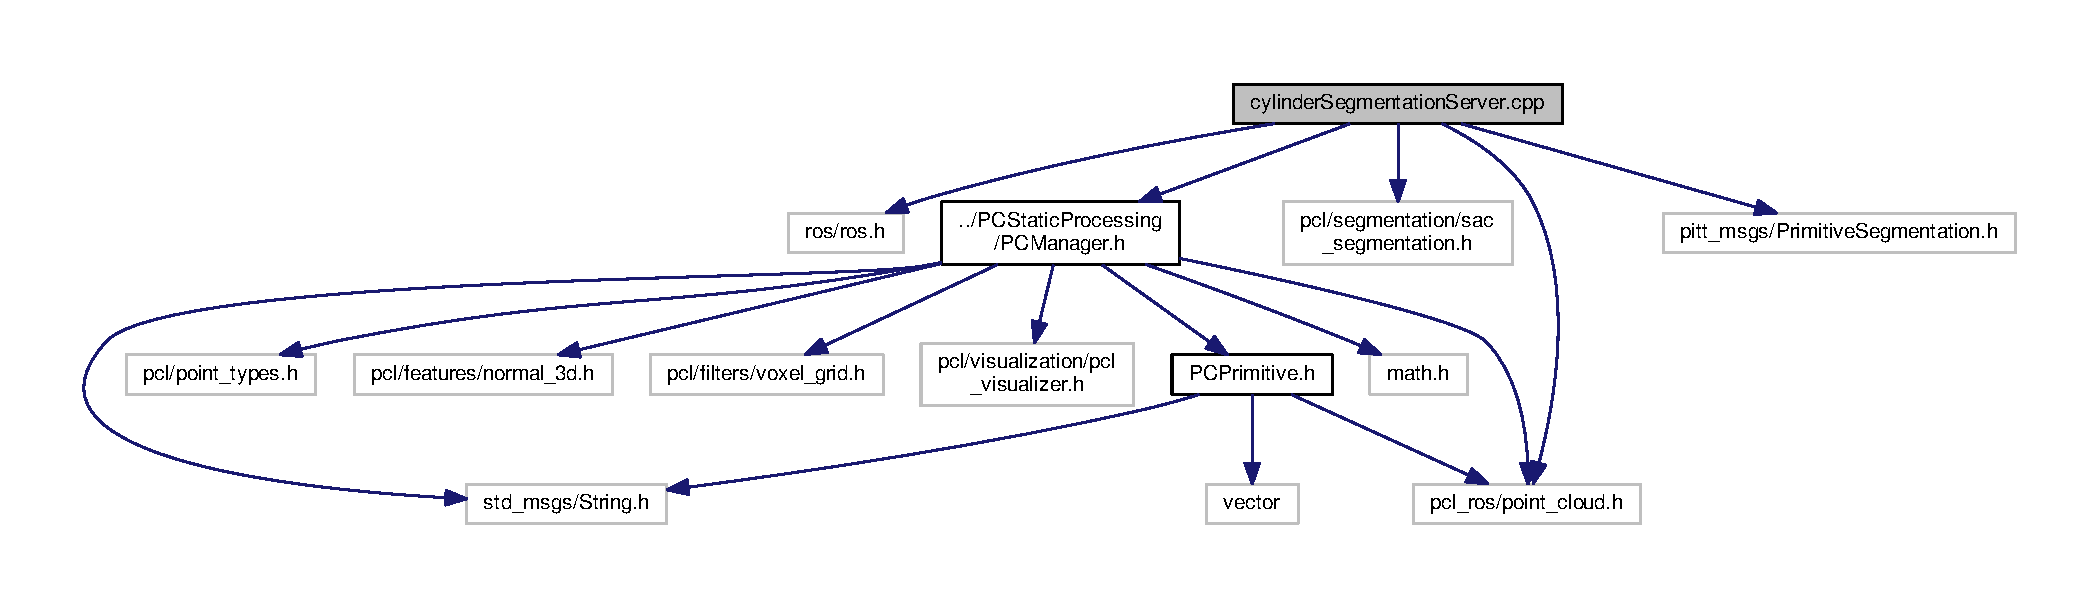
\includegraphics[width=350pt]{cylinderSegmentationServer_8cpp__incl}
\end{center}
\end{figure}
\subsection*{Classes}
\begin{DoxyCompactItemize}
\item 
struct \hyperlink{structvector3d}{vector3d}
\end{DoxyCompactItemize}
\subsection*{Functions}
\begin{DoxyCompactItemize}
\item 
\hyperlink{structvector3d}{vector3d} \hyperlink{cylinderSegmentationServer_8cpp_a18fcf7fa2e84ef1176c2ca1abed744cf}{get\-Normalize\-Axes\-Direction\-Vector} (Model\-Coefficients\-::\-Ptr coefficients)
\item 
\hyperlink{structvector3d}{vector3d} \hyperlink{cylinderSegmentationServer_8cpp_a255909b8e4ba570eea6756718bf79df1}{get\-Point\-On\-Axes} (Model\-Coefficients\-::\-Ptr coefficients, \hyperlink{structvector3d}{vector3d} direction, float t)
\item 
\hyperlink{structvector3d}{vector3d} \hyperlink{cylinderSegmentationServer_8cpp_a00c9eb33d55847838be7bf32c23d1893}{get\-Vector\-Between\-Points} (\hyperlink{structvector3d}{vector3d} p1, \hyperlink{structvector3d}{vector3d} p2)
\item 
bool \hyperlink{cylinderSegmentationServer_8cpp_a1c3f80670f74628ec0f4bfb28fe2bc10}{ransac\-Cylinder\-Detaction} (Primitive\-Segmentation\-::\-Request \&req, Primitive\-Segmentation\-::\-Response \&res)
\item 
int \hyperlink{cylinderSegmentationServer_8cpp_a3c04138a5bfe5d72780bb7e82a18e627}{main} (int argc, char $\ast$$\ast$argv)
\end{DoxyCompactItemize}
\subsection*{Variables}
\begin{DoxyCompactItemize}
\item 
const float \hyperlink{cylinderSegmentationServer_8cpp_a6a60b5e5200860d75f403dcf05dde9ef}{N\-O\-R\-M\-A\-L\-\_\-\-D\-I\-S\-T\-A\-N\-C\-E\-\_\-\-W\-E\-I\-G\-H\-T\-\_\-\-D\-E\-F\-A\-U\-L\-T} = 0.\-001f
\item 
const float \hyperlink{cylinderSegmentationServer_8cpp_a73e7be3a150e91558f7c5e69c03dd6e6}{D\-I\-S\-T\-A\-N\-C\-E\-\_\-\-T\-H\-R\-E\-S\-H\-O\-L\-D\-\_\-\-D\-E\-F\-A\-U\-L\-T} = 0.\-008f
\item 
const int \hyperlink{cylinderSegmentationServer_8cpp_aeb805bfa6116e2c314b0ebc3c73c6504}{M\-A\-X\-\_\-\-I\-T\-E\-R\-A\-T\-I\-O\-N\-\_\-\-D\-E\-F\-A\-U\-L\-T} = 1000
\item 
const float \hyperlink{cylinderSegmentationServer_8cpp_aa84d6979d2a503e253f54c3e069abaf5}{M\-I\-N\-\_\-\-R\-A\-D\-I\-U\-S\-\_\-\-L\-I\-M\-I\-T} = 0.\-005
\item 
const float \hyperlink{cylinderSegmentationServer_8cpp_abcdbdc04946f1566041df18c6c892f0f}{M\-A\-X\-\_\-\-R\-A\-D\-I\-U\-S\-\_\-\-L\-I\-M\-I\-T} = 0.\-500
\item 
const float \hyperlink{cylinderSegmentationServer_8cpp_a32a067fb9ad7cc8e19b52018946d374d}{E\-P\-S\-\_\-\-A\-N\-G\-L\-E} = 0.\-0001f
\item 
const float \hyperlink{cylinderSegmentationServer_8cpp_ae71c4fb043a78285d76d4dcbd7231e70}{M\-I\-N\-\_\-\-O\-P\-E\-N\-I\-N\-G\-\_\-\-A\-N\-G\-L\-E} = 50.\-0f
\item 
const float \hyperlink{cylinderSegmentationServer_8cpp_afaeeefd6f578a58f8e14040f6176c394}{M\-A\-X\-\_\-\-O\-P\-E\-N\-I\-N\-G\-\_\-\-A\-N\-G\-L\-E} = 180.\-0f
\item 
const bool \hyperlink{cylinderSegmentationServer_8cpp_a20f88026cd9df482d817a3868c20fe43}{V\-I\-S\-U\-A\-L\-I\-Z\-E\-\_\-\-R\-E\-S\-U\-L\-T} = false
\item 
boost\-::shared\-\_\-ptr\\*
$<$ \hyperlink{PCManager_8h_a38c805dbc7ad6f06109b85c8e540817a}{visualization\-::\-P\-C\-L\-Visualizer} $>$ \hyperlink{cylinderSegmentationServer_8cpp_a6c2d87234fca8dcca11f888098558986}{vis}
\end{DoxyCompactItemize}


\subsection{Function Documentation}
\hypertarget{cylinderSegmentationServer_8cpp_a18fcf7fa2e84ef1176c2ca1abed744cf}{\index{cylinder\-Segmentation\-Server.\-cpp@{cylinder\-Segmentation\-Server.\-cpp}!get\-Normalize\-Axes\-Direction\-Vector@{get\-Normalize\-Axes\-Direction\-Vector}}
\index{get\-Normalize\-Axes\-Direction\-Vector@{get\-Normalize\-Axes\-Direction\-Vector}!cylinderSegmentationServer.cpp@{cylinder\-Segmentation\-Server.\-cpp}}
\subsubsection[{get\-Normalize\-Axes\-Direction\-Vector}]{\setlength{\rightskip}{0pt plus 5cm}{\bf vector3d} get\-Normalize\-Axes\-Direction\-Vector (
\begin{DoxyParamCaption}
\item[{Model\-Coefficients\-::\-Ptr}]{coefficients}
\end{DoxyParamCaption}
)}}\label{cylinderSegmentationServer_8cpp_a18fcf7fa2e84ef1176c2ca1abed744cf}


Definition at line 37 of file cylinder\-Segmentation\-Server.\-cpp.



References vector3d\-::x, vector3d\-::y, and vector3d\-::z.



Referenced by ransac\-Cylinder\-Detaction().

\hypertarget{cylinderSegmentationServer_8cpp_a255909b8e4ba570eea6756718bf79df1}{\index{cylinder\-Segmentation\-Server.\-cpp@{cylinder\-Segmentation\-Server.\-cpp}!get\-Point\-On\-Axes@{get\-Point\-On\-Axes}}
\index{get\-Point\-On\-Axes@{get\-Point\-On\-Axes}!cylinderSegmentationServer.cpp@{cylinder\-Segmentation\-Server.\-cpp}}
\subsubsection[{get\-Point\-On\-Axes}]{\setlength{\rightskip}{0pt plus 5cm}{\bf vector3d} get\-Point\-On\-Axes (
\begin{DoxyParamCaption}
\item[{Model\-Coefficients\-::\-Ptr}]{coefficients, }
\item[{{\bf vector3d}}]{direction, }
\item[{float}]{t}
\end{DoxyParamCaption}
)}}\label{cylinderSegmentationServer_8cpp_a255909b8e4ba570eea6756718bf79df1}


Definition at line 48 of file cylinder\-Segmentation\-Server.\-cpp.



References vector3d\-::x, vector3d\-::y, and vector3d\-::z.



Referenced by ransac\-Cylinder\-Detaction().

\hypertarget{cylinderSegmentationServer_8cpp_a00c9eb33d55847838be7bf32c23d1893}{\index{cylinder\-Segmentation\-Server.\-cpp@{cylinder\-Segmentation\-Server.\-cpp}!get\-Vector\-Between\-Points@{get\-Vector\-Between\-Points}}
\index{get\-Vector\-Between\-Points@{get\-Vector\-Between\-Points}!cylinderSegmentationServer.cpp@{cylinder\-Segmentation\-Server.\-cpp}}
\subsubsection[{get\-Vector\-Between\-Points}]{\setlength{\rightskip}{0pt plus 5cm}{\bf vector3d} get\-Vector\-Between\-Points (
\begin{DoxyParamCaption}
\item[{{\bf vector3d}}]{p1, }
\item[{{\bf vector3d}}]{p2}
\end{DoxyParamCaption}
)}}\label{cylinderSegmentationServer_8cpp_a00c9eb33d55847838be7bf32c23d1893}


Definition at line 57 of file cylinder\-Segmentation\-Server.\-cpp.



References vector3d\-::x, vector3d\-::y, and vector3d\-::z.



Referenced by ransac\-Cylinder\-Detaction().

\hypertarget{cylinderSegmentationServer_8cpp_a3c04138a5bfe5d72780bb7e82a18e627}{\index{cylinder\-Segmentation\-Server.\-cpp@{cylinder\-Segmentation\-Server.\-cpp}!main@{main}}
\index{main@{main}!cylinderSegmentationServer.cpp@{cylinder\-Segmentation\-Server.\-cpp}}
\subsubsection[{main}]{\setlength{\rightskip}{0pt plus 5cm}int main (
\begin{DoxyParamCaption}
\item[{int}]{argc, }
\item[{char $\ast$$\ast$}]{argv}
\end{DoxyParamCaption}
)}}\label{cylinderSegmentationServer_8cpp_a3c04138a5bfe5d72780bb7e82a18e627}


Definition at line 220 of file cylinder\-Segmentation\-Server.\-cpp.



References pcm\-::\-P\-C\-Manager\-::create\-Visor(), pcm\-::\-P\-C\-Manager\-::\-R\-A\-N\-S\-A\-C\-\_\-\-C\-Y\-L\-I\-N\-D\-E\-R\-\_\-\-F\-I\-L\-T\-E\-R\-\_\-\-S\-E\-R\-V\-I\-C\-E\-\_\-\-N\-A\-M\-E, ransac\-Cylinder\-Detaction(), vis, and V\-I\-S\-U\-A\-L\-I\-Z\-E\-\_\-\-R\-E\-S\-U\-L\-T.



Here is the call graph for this function\-:\nopagebreak
\begin{figure}[H]
\begin{center}
\leavevmode
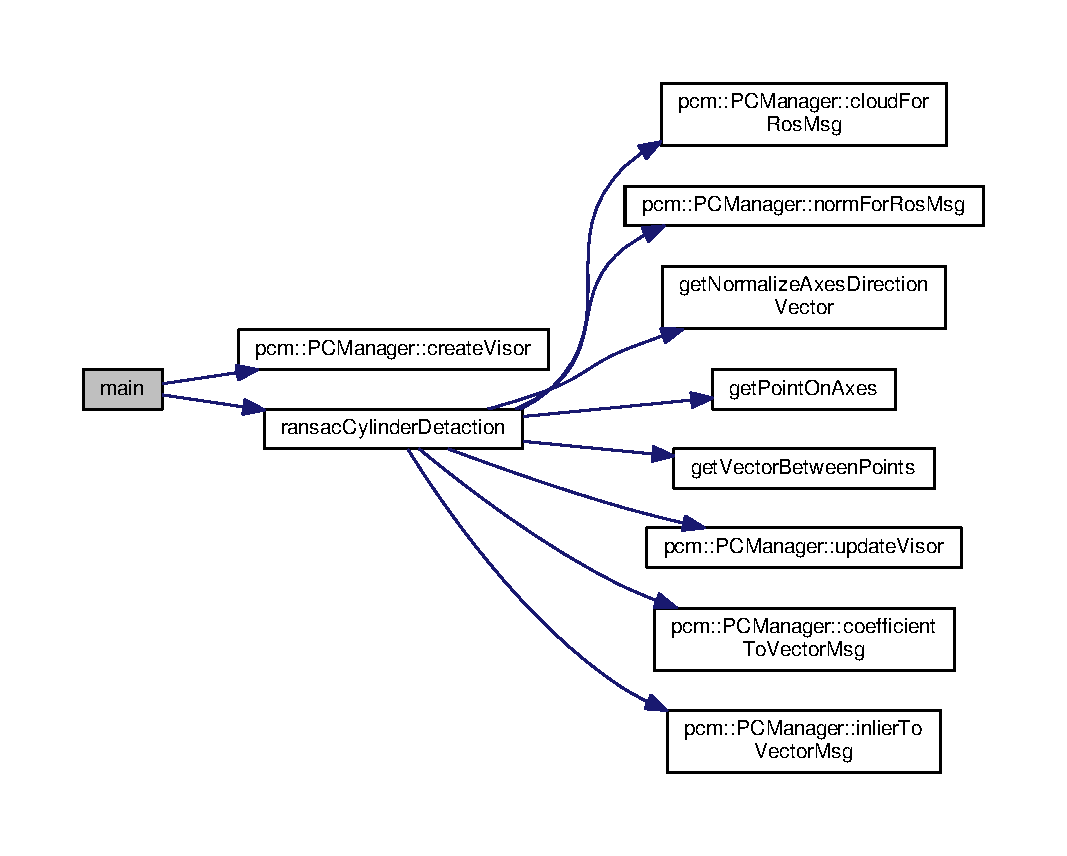
\includegraphics[width=350pt]{cylinderSegmentationServer_8cpp_a3c04138a5bfe5d72780bb7e82a18e627_cgraph}
\end{center}
\end{figure}


\hypertarget{cylinderSegmentationServer_8cpp_a1c3f80670f74628ec0f4bfb28fe2bc10}{\index{cylinder\-Segmentation\-Server.\-cpp@{cylinder\-Segmentation\-Server.\-cpp}!ransac\-Cylinder\-Detaction@{ransac\-Cylinder\-Detaction}}
\index{ransac\-Cylinder\-Detaction@{ransac\-Cylinder\-Detaction}!cylinderSegmentationServer.cpp@{cylinder\-Segmentation\-Server.\-cpp}}
\subsubsection[{ransac\-Cylinder\-Detaction}]{\setlength{\rightskip}{0pt plus 5cm}bool ransac\-Cylinder\-Detaction (
\begin{DoxyParamCaption}
\item[{Primitive\-Segmentation\-::\-Request \&}]{req, }
\item[{Primitive\-Segmentation\-::\-Response \&}]{res}
\end{DoxyParamCaption}
)}}\label{cylinderSegmentationServer_8cpp_a1c3f80670f74628ec0f4bfb28fe2bc10}


Definition at line 66 of file cylinder\-Segmentation\-Server.\-cpp.



References pcm\-::\-P\-C\-Manager\-::cloud\-For\-Ros\-Msg(), pcm\-::\-P\-C\-Manager\-::coefficient\-To\-Vector\-Msg(), D\-I\-S\-T\-A\-N\-C\-E\-\_\-\-T\-H\-R\-E\-S\-H\-O\-L\-D\-\_\-\-D\-E\-F\-A\-U\-L\-T, E\-P\-S\-\_\-\-A\-N\-G\-L\-E, get\-Normalize\-Axes\-Direction\-Vector(), get\-Point\-On\-Axes(), get\-Vector\-Between\-Points(), pcm\-::\-P\-C\-Manager\-::inlier\-To\-Vector\-Msg(), M\-A\-X\-\_\-\-I\-T\-E\-R\-A\-T\-I\-O\-N\-\_\-\-D\-E\-F\-A\-U\-L\-T, M\-A\-X\-\_\-\-O\-P\-E\-N\-I\-N\-G\-\_\-\-A\-N\-G\-L\-E, M\-A\-X\-\_\-\-R\-A\-D\-I\-U\-S\-\_\-\-L\-I\-M\-I\-T, M\-I\-N\-\_\-\-O\-P\-E\-N\-I\-N\-G\-\_\-\-A\-N\-G\-L\-E, M\-I\-N\-\_\-\-R\-A\-D\-I\-U\-S\-\_\-\-L\-I\-M\-I\-T, N\-O\-R\-M\-A\-L\-\_\-\-D\-I\-S\-T\-A\-N\-C\-E\-\_\-\-W\-E\-I\-G\-H\-T\-\_\-\-D\-E\-F\-A\-U\-L\-T, pcm\-::\-P\-C\-Manager\-::norm\-For\-Ros\-Msg(), seg, pcm\-::\-P\-C\-Manager\-::update\-Visor(), vis, V\-I\-S\-U\-A\-L\-I\-Z\-E\-\_\-\-R\-E\-S\-U\-L\-T, vector3d\-::x, vector3d\-::y, and vector3d\-::z.



Referenced by main().



Here is the call graph for this function\-:\nopagebreak
\begin{figure}[H]
\begin{center}
\leavevmode
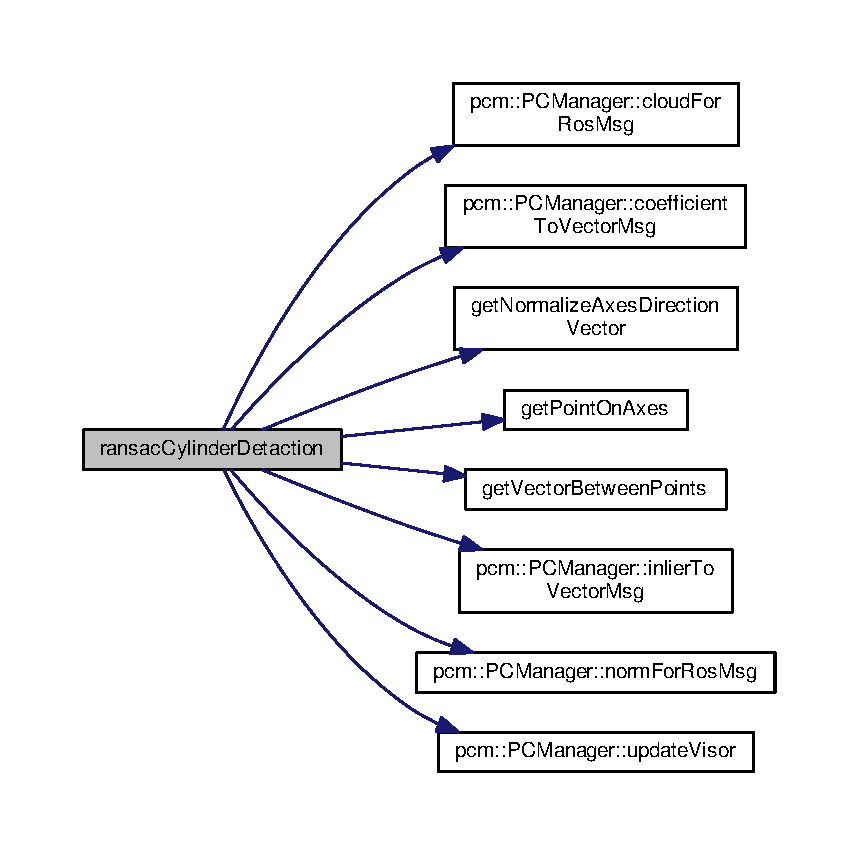
\includegraphics[width=350pt]{cylinderSegmentationServer_8cpp_a1c3f80670f74628ec0f4bfb28fe2bc10_cgraph}
\end{center}
\end{figure}




\subsection{Variable Documentation}
\hypertarget{cylinderSegmentationServer_8cpp_a73e7be3a150e91558f7c5e69c03dd6e6}{\index{cylinder\-Segmentation\-Server.\-cpp@{cylinder\-Segmentation\-Server.\-cpp}!D\-I\-S\-T\-A\-N\-C\-E\-\_\-\-T\-H\-R\-E\-S\-H\-O\-L\-D\-\_\-\-D\-E\-F\-A\-U\-L\-T@{D\-I\-S\-T\-A\-N\-C\-E\-\_\-\-T\-H\-R\-E\-S\-H\-O\-L\-D\-\_\-\-D\-E\-F\-A\-U\-L\-T}}
\index{D\-I\-S\-T\-A\-N\-C\-E\-\_\-\-T\-H\-R\-E\-S\-H\-O\-L\-D\-\_\-\-D\-E\-F\-A\-U\-L\-T@{D\-I\-S\-T\-A\-N\-C\-E\-\_\-\-T\-H\-R\-E\-S\-H\-O\-L\-D\-\_\-\-D\-E\-F\-A\-U\-L\-T}!cylinderSegmentationServer.cpp@{cylinder\-Segmentation\-Server.\-cpp}}
\subsubsection[{D\-I\-S\-T\-A\-N\-C\-E\-\_\-\-T\-H\-R\-E\-S\-H\-O\-L\-D\-\_\-\-D\-E\-F\-A\-U\-L\-T}]{\setlength{\rightskip}{0pt plus 5cm}const float D\-I\-S\-T\-A\-N\-C\-E\-\_\-\-T\-H\-R\-E\-S\-H\-O\-L\-D\-\_\-\-D\-E\-F\-A\-U\-L\-T = 0.\-008f}}\label{cylinderSegmentationServer_8cpp_a73e7be3a150e91558f7c5e69c03dd6e6}


Definition at line 17 of file cylinder\-Segmentation\-Server.\-cpp.



Referenced by ransac\-Cylinder\-Detaction().

\hypertarget{cylinderSegmentationServer_8cpp_a32a067fb9ad7cc8e19b52018946d374d}{\index{cylinder\-Segmentation\-Server.\-cpp@{cylinder\-Segmentation\-Server.\-cpp}!E\-P\-S\-\_\-\-A\-N\-G\-L\-E@{E\-P\-S\-\_\-\-A\-N\-G\-L\-E}}
\index{E\-P\-S\-\_\-\-A\-N\-G\-L\-E@{E\-P\-S\-\_\-\-A\-N\-G\-L\-E}!cylinderSegmentationServer.cpp@{cylinder\-Segmentation\-Server.\-cpp}}
\subsubsection[{E\-P\-S\-\_\-\-A\-N\-G\-L\-E}]{\setlength{\rightskip}{0pt plus 5cm}const float E\-P\-S\-\_\-\-A\-N\-G\-L\-E = 0.\-0001f}}\label{cylinderSegmentationServer_8cpp_a32a067fb9ad7cc8e19b52018946d374d}


Definition at line 21 of file cylinder\-Segmentation\-Server.\-cpp.



Referenced by ransac\-Cylinder\-Detaction().

\hypertarget{cylinderSegmentationServer_8cpp_aeb805bfa6116e2c314b0ebc3c73c6504}{\index{cylinder\-Segmentation\-Server.\-cpp@{cylinder\-Segmentation\-Server.\-cpp}!M\-A\-X\-\_\-\-I\-T\-E\-R\-A\-T\-I\-O\-N\-\_\-\-D\-E\-F\-A\-U\-L\-T@{M\-A\-X\-\_\-\-I\-T\-E\-R\-A\-T\-I\-O\-N\-\_\-\-D\-E\-F\-A\-U\-L\-T}}
\index{M\-A\-X\-\_\-\-I\-T\-E\-R\-A\-T\-I\-O\-N\-\_\-\-D\-E\-F\-A\-U\-L\-T@{M\-A\-X\-\_\-\-I\-T\-E\-R\-A\-T\-I\-O\-N\-\_\-\-D\-E\-F\-A\-U\-L\-T}!cylinderSegmentationServer.cpp@{cylinder\-Segmentation\-Server.\-cpp}}
\subsubsection[{M\-A\-X\-\_\-\-I\-T\-E\-R\-A\-T\-I\-O\-N\-\_\-\-D\-E\-F\-A\-U\-L\-T}]{\setlength{\rightskip}{0pt plus 5cm}const int M\-A\-X\-\_\-\-I\-T\-E\-R\-A\-T\-I\-O\-N\-\_\-\-D\-E\-F\-A\-U\-L\-T = 1000}}\label{cylinderSegmentationServer_8cpp_aeb805bfa6116e2c314b0ebc3c73c6504}


Definition at line 18 of file cylinder\-Segmentation\-Server.\-cpp.



Referenced by ransac\-Cylinder\-Detaction().

\hypertarget{cylinderSegmentationServer_8cpp_afaeeefd6f578a58f8e14040f6176c394}{\index{cylinder\-Segmentation\-Server.\-cpp@{cylinder\-Segmentation\-Server.\-cpp}!M\-A\-X\-\_\-\-O\-P\-E\-N\-I\-N\-G\-\_\-\-A\-N\-G\-L\-E@{M\-A\-X\-\_\-\-O\-P\-E\-N\-I\-N\-G\-\_\-\-A\-N\-G\-L\-E}}
\index{M\-A\-X\-\_\-\-O\-P\-E\-N\-I\-N\-G\-\_\-\-A\-N\-G\-L\-E@{M\-A\-X\-\_\-\-O\-P\-E\-N\-I\-N\-G\-\_\-\-A\-N\-G\-L\-E}!cylinderSegmentationServer.cpp@{cylinder\-Segmentation\-Server.\-cpp}}
\subsubsection[{M\-A\-X\-\_\-\-O\-P\-E\-N\-I\-N\-G\-\_\-\-A\-N\-G\-L\-E}]{\setlength{\rightskip}{0pt plus 5cm}const float M\-A\-X\-\_\-\-O\-P\-E\-N\-I\-N\-G\-\_\-\-A\-N\-G\-L\-E = 180.\-0f}}\label{cylinderSegmentationServer_8cpp_afaeeefd6f578a58f8e14040f6176c394}


Definition at line 23 of file cylinder\-Segmentation\-Server.\-cpp.



Referenced by ransac\-Cylinder\-Detaction().

\hypertarget{cylinderSegmentationServer_8cpp_abcdbdc04946f1566041df18c6c892f0f}{\index{cylinder\-Segmentation\-Server.\-cpp@{cylinder\-Segmentation\-Server.\-cpp}!M\-A\-X\-\_\-\-R\-A\-D\-I\-U\-S\-\_\-\-L\-I\-M\-I\-T@{M\-A\-X\-\_\-\-R\-A\-D\-I\-U\-S\-\_\-\-L\-I\-M\-I\-T}}
\index{M\-A\-X\-\_\-\-R\-A\-D\-I\-U\-S\-\_\-\-L\-I\-M\-I\-T@{M\-A\-X\-\_\-\-R\-A\-D\-I\-U\-S\-\_\-\-L\-I\-M\-I\-T}!cylinderSegmentationServer.cpp@{cylinder\-Segmentation\-Server.\-cpp}}
\subsubsection[{M\-A\-X\-\_\-\-R\-A\-D\-I\-U\-S\-\_\-\-L\-I\-M\-I\-T}]{\setlength{\rightskip}{0pt plus 5cm}const float M\-A\-X\-\_\-\-R\-A\-D\-I\-U\-S\-\_\-\-L\-I\-M\-I\-T = 0.\-500}}\label{cylinderSegmentationServer_8cpp_abcdbdc04946f1566041df18c6c892f0f}


Definition at line 20 of file cylinder\-Segmentation\-Server.\-cpp.



Referenced by ransac\-Cylinder\-Detaction().

\hypertarget{cylinderSegmentationServer_8cpp_ae71c4fb043a78285d76d4dcbd7231e70}{\index{cylinder\-Segmentation\-Server.\-cpp@{cylinder\-Segmentation\-Server.\-cpp}!M\-I\-N\-\_\-\-O\-P\-E\-N\-I\-N\-G\-\_\-\-A\-N\-G\-L\-E@{M\-I\-N\-\_\-\-O\-P\-E\-N\-I\-N\-G\-\_\-\-A\-N\-G\-L\-E}}
\index{M\-I\-N\-\_\-\-O\-P\-E\-N\-I\-N\-G\-\_\-\-A\-N\-G\-L\-E@{M\-I\-N\-\_\-\-O\-P\-E\-N\-I\-N\-G\-\_\-\-A\-N\-G\-L\-E}!cylinderSegmentationServer.cpp@{cylinder\-Segmentation\-Server.\-cpp}}
\subsubsection[{M\-I\-N\-\_\-\-O\-P\-E\-N\-I\-N\-G\-\_\-\-A\-N\-G\-L\-E}]{\setlength{\rightskip}{0pt plus 5cm}const float M\-I\-N\-\_\-\-O\-P\-E\-N\-I\-N\-G\-\_\-\-A\-N\-G\-L\-E = 50.\-0f}}\label{cylinderSegmentationServer_8cpp_ae71c4fb043a78285d76d4dcbd7231e70}


Definition at line 22 of file cylinder\-Segmentation\-Server.\-cpp.



Referenced by ransac\-Cylinder\-Detaction().

\hypertarget{cylinderSegmentationServer_8cpp_aa84d6979d2a503e253f54c3e069abaf5}{\index{cylinder\-Segmentation\-Server.\-cpp@{cylinder\-Segmentation\-Server.\-cpp}!M\-I\-N\-\_\-\-R\-A\-D\-I\-U\-S\-\_\-\-L\-I\-M\-I\-T@{M\-I\-N\-\_\-\-R\-A\-D\-I\-U\-S\-\_\-\-L\-I\-M\-I\-T}}
\index{M\-I\-N\-\_\-\-R\-A\-D\-I\-U\-S\-\_\-\-L\-I\-M\-I\-T@{M\-I\-N\-\_\-\-R\-A\-D\-I\-U\-S\-\_\-\-L\-I\-M\-I\-T}!cylinderSegmentationServer.cpp@{cylinder\-Segmentation\-Server.\-cpp}}
\subsubsection[{M\-I\-N\-\_\-\-R\-A\-D\-I\-U\-S\-\_\-\-L\-I\-M\-I\-T}]{\setlength{\rightskip}{0pt plus 5cm}const float M\-I\-N\-\_\-\-R\-A\-D\-I\-U\-S\-\_\-\-L\-I\-M\-I\-T = 0.\-005}}\label{cylinderSegmentationServer_8cpp_aa84d6979d2a503e253f54c3e069abaf5}


Definition at line 19 of file cylinder\-Segmentation\-Server.\-cpp.



Referenced by ransac\-Cylinder\-Detaction().

\hypertarget{cylinderSegmentationServer_8cpp_a6a60b5e5200860d75f403dcf05dde9ef}{\index{cylinder\-Segmentation\-Server.\-cpp@{cylinder\-Segmentation\-Server.\-cpp}!N\-O\-R\-M\-A\-L\-\_\-\-D\-I\-S\-T\-A\-N\-C\-E\-\_\-\-W\-E\-I\-G\-H\-T\-\_\-\-D\-E\-F\-A\-U\-L\-T@{N\-O\-R\-M\-A\-L\-\_\-\-D\-I\-S\-T\-A\-N\-C\-E\-\_\-\-W\-E\-I\-G\-H\-T\-\_\-\-D\-E\-F\-A\-U\-L\-T}}
\index{N\-O\-R\-M\-A\-L\-\_\-\-D\-I\-S\-T\-A\-N\-C\-E\-\_\-\-W\-E\-I\-G\-H\-T\-\_\-\-D\-E\-F\-A\-U\-L\-T@{N\-O\-R\-M\-A\-L\-\_\-\-D\-I\-S\-T\-A\-N\-C\-E\-\_\-\-W\-E\-I\-G\-H\-T\-\_\-\-D\-E\-F\-A\-U\-L\-T}!cylinderSegmentationServer.cpp@{cylinder\-Segmentation\-Server.\-cpp}}
\subsubsection[{N\-O\-R\-M\-A\-L\-\_\-\-D\-I\-S\-T\-A\-N\-C\-E\-\_\-\-W\-E\-I\-G\-H\-T\-\_\-\-D\-E\-F\-A\-U\-L\-T}]{\setlength{\rightskip}{0pt plus 5cm}const float N\-O\-R\-M\-A\-L\-\_\-\-D\-I\-S\-T\-A\-N\-C\-E\-\_\-\-W\-E\-I\-G\-H\-T\-\_\-\-D\-E\-F\-A\-U\-L\-T = 0.\-001f}}\label{cylinderSegmentationServer_8cpp_a6a60b5e5200860d75f403dcf05dde9ef}


Definition at line 16 of file cylinder\-Segmentation\-Server.\-cpp.



Referenced by ransac\-Cylinder\-Detaction().

\hypertarget{cylinderSegmentationServer_8cpp_a6c2d87234fca8dcca11f888098558986}{\index{cylinder\-Segmentation\-Server.\-cpp@{cylinder\-Segmentation\-Server.\-cpp}!vis@{vis}}
\index{vis@{vis}!cylinderSegmentationServer.cpp@{cylinder\-Segmentation\-Server.\-cpp}}
\subsubsection[{vis}]{\setlength{\rightskip}{0pt plus 5cm}boost\-::shared\-\_\-ptr$<$ {\bf visualization\-::\-P\-C\-L\-Visualizer}$>$ vis}}\label{cylinderSegmentationServer_8cpp_a6c2d87234fca8dcca11f888098558986}


Definition at line 34 of file cylinder\-Segmentation\-Server.\-cpp.



Referenced by main(), and ransac\-Cylinder\-Detaction().

\hypertarget{cylinderSegmentationServer_8cpp_a20f88026cd9df482d817a3868c20fe43}{\index{cylinder\-Segmentation\-Server.\-cpp@{cylinder\-Segmentation\-Server.\-cpp}!V\-I\-S\-U\-A\-L\-I\-Z\-E\-\_\-\-R\-E\-S\-U\-L\-T@{V\-I\-S\-U\-A\-L\-I\-Z\-E\-\_\-\-R\-E\-S\-U\-L\-T}}
\index{V\-I\-S\-U\-A\-L\-I\-Z\-E\-\_\-\-R\-E\-S\-U\-L\-T@{V\-I\-S\-U\-A\-L\-I\-Z\-E\-\_\-\-R\-E\-S\-U\-L\-T}!cylinderSegmentationServer.cpp@{cylinder\-Segmentation\-Server.\-cpp}}
\subsubsection[{V\-I\-S\-U\-A\-L\-I\-Z\-E\-\_\-\-R\-E\-S\-U\-L\-T}]{\setlength{\rightskip}{0pt plus 5cm}const bool V\-I\-S\-U\-A\-L\-I\-Z\-E\-\_\-\-R\-E\-S\-U\-L\-T = false}}\label{cylinderSegmentationServer_8cpp_a20f88026cd9df482d817a3868c20fe43}


Definition at line 33 of file cylinder\-Segmentation\-Server.\-cpp.



Referenced by main(), and ransac\-Cylinder\-Detaction().


\hypertarget{deepFilterServer_8cpp}{\section{deep\-Filter\-Server.\-cpp File Reference}
\label{deepFilterServer_8cpp}\index{deep\-Filter\-Server.\-cpp@{deep\-Filter\-Server.\-cpp}}
}
{\ttfamily \#include \char`\"{}ros/ros.\-h\char`\"{}}\\*
{\ttfamily \#include $<$iostream$>$}\\*
{\ttfamily \#include \char`\"{}pitt\-\_\-msgs/\-Deep\-Filter.\-h\char`\"{}}\\*
{\ttfamily \#include \char`\"{}../\-P\-C\-Static\-Processing/\-P\-C\-Manager.\-h\char`\"{}}\\*
Include dependency graph for deep\-Filter\-Server.\-cpp\-:\nopagebreak
\begin{figure}[H]
\begin{center}
\leavevmode
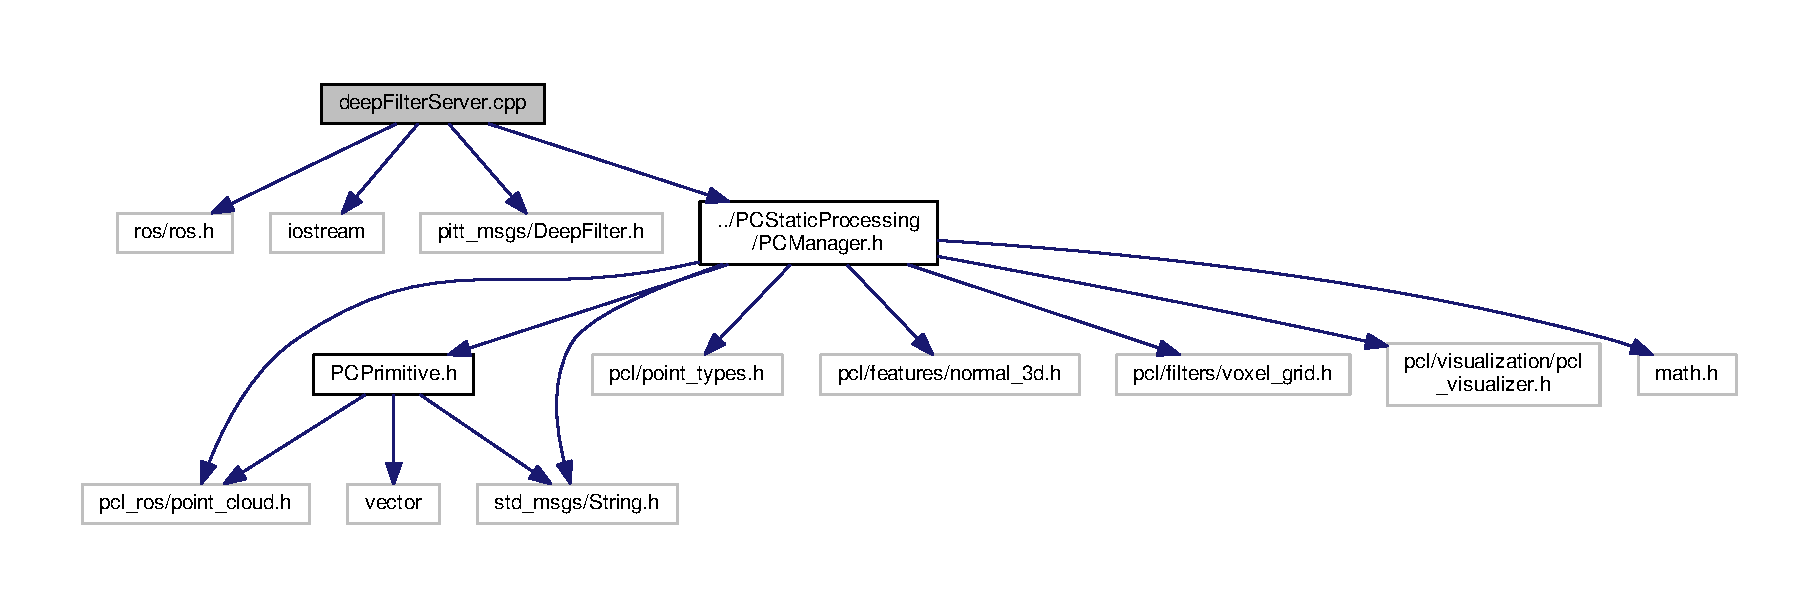
\includegraphics[width=350pt]{deepFilterServer_8cpp__incl}
\end{center}
\end{figure}
\subsection*{Functions}
\begin{DoxyCompactItemize}
\item 
bool \hyperlink{deepFilterServer_8cpp_a09a168bce8338d7fd9b6f350b98d37c8}{deep\-Filtering} (Deep\-Filter\-::\-Request \&req, Deep\-Filter\-::\-Response \&res)
\item 
int \hyperlink{deepFilterServer_8cpp_a3c04138a5bfe5d72780bb7e82a18e627}{main} (int argc, char $\ast$$\ast$argv)
\end{DoxyCompactItemize}
\subsection*{Variables}
\begin{DoxyCompactItemize}
\item 
static const float \hyperlink{deepFilterServer_8cpp_a557d1794ec1b495e35d2d4a4373400f3}{D\-E\-P\-T\-H\-\_\-\-T\-H\-R\-E\-S\-H\-O\-U\-L\-D} = 3.\-000f
\end{DoxyCompactItemize}


\subsection{Function Documentation}
\hypertarget{deepFilterServer_8cpp_a09a168bce8338d7fd9b6f350b98d37c8}{\index{deep\-Filter\-Server.\-cpp@{deep\-Filter\-Server.\-cpp}!deep\-Filtering@{deep\-Filtering}}
\index{deep\-Filtering@{deep\-Filtering}!deepFilterServer.cpp@{deep\-Filter\-Server.\-cpp}}
\subsubsection[{deep\-Filtering}]{\setlength{\rightskip}{0pt plus 5cm}bool deep\-Filtering (
\begin{DoxyParamCaption}
\item[{Deep\-Filter\-::\-Request \&}]{req, }
\item[{Deep\-Filter\-::\-Response \&}]{res}
\end{DoxyParamCaption}
)}}\label{deepFilterServer_8cpp_a09a168bce8338d7fd9b6f350b98d37c8}


Definition at line 29 of file deep\-Filter\-Server.\-cpp.



References D\-E\-P\-T\-H\-\_\-\-T\-H\-R\-E\-S\-H\-O\-U\-L\-D.



Referenced by main().

\hypertarget{deepFilterServer_8cpp_a3c04138a5bfe5d72780bb7e82a18e627}{\index{deep\-Filter\-Server.\-cpp@{deep\-Filter\-Server.\-cpp}!main@{main}}
\index{main@{main}!deepFilterServer.cpp@{deep\-Filter\-Server.\-cpp}}
\subsubsection[{main}]{\setlength{\rightskip}{0pt plus 5cm}int main (
\begin{DoxyParamCaption}
\item[{int}]{argc, }
\item[{char $\ast$$\ast$}]{argv}
\end{DoxyParamCaption}
)}}\label{deepFilterServer_8cpp_a3c04138a5bfe5d72780bb7e82a18e627}


Definition at line 64 of file deep\-Filter\-Server.\-cpp.



References deep\-Filtering().



Here is the call graph for this function\-:\nopagebreak
\begin{figure}[H]
\begin{center}
\leavevmode
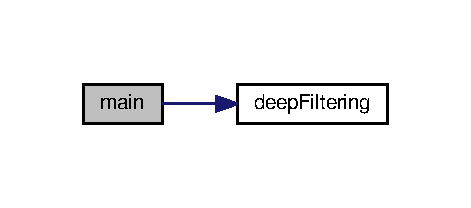
\includegraphics[width=226pt]{deepFilterServer_8cpp_a3c04138a5bfe5d72780bb7e82a18e627_cgraph}
\end{center}
\end{figure}




\subsection{Variable Documentation}
\hypertarget{deepFilterServer_8cpp_a557d1794ec1b495e35d2d4a4373400f3}{\index{deep\-Filter\-Server.\-cpp@{deep\-Filter\-Server.\-cpp}!D\-E\-P\-T\-H\-\_\-\-T\-H\-R\-E\-S\-H\-O\-U\-L\-D@{D\-E\-P\-T\-H\-\_\-\-T\-H\-R\-E\-S\-H\-O\-U\-L\-D}}
\index{D\-E\-P\-T\-H\-\_\-\-T\-H\-R\-E\-S\-H\-O\-U\-L\-D@{D\-E\-P\-T\-H\-\_\-\-T\-H\-R\-E\-S\-H\-O\-U\-L\-D}!deepFilterServer.cpp@{deep\-Filter\-Server.\-cpp}}
\subsubsection[{D\-E\-P\-T\-H\-\_\-\-T\-H\-R\-E\-S\-H\-O\-U\-L\-D}]{\setlength{\rightskip}{0pt plus 5cm}const float D\-E\-P\-T\-H\-\_\-\-T\-H\-R\-E\-S\-H\-O\-U\-L\-D = 3.\-000f\hspace{0.3cm}{\ttfamily [static]}}}\label{deepFilterServer_8cpp_a557d1794ec1b495e35d2d4a4373400f3}


Definition at line 24 of file deep\-Filter\-Server.\-cpp.



Referenced by deep\-Filtering().


\hypertarget{introduction_8dox}{\section{introduction.\-dox File Reference}
\label{introduction_8dox}\index{introduction.\-dox@{introduction.\-dox}}
}

\hypertarget{obj__segmentation_8cpp}{\section{obj\-\_\-segmentation.\-cpp File Reference}
\label{obj__segmentation_8cpp}\index{obj\-\_\-segmentation.\-cpp@{obj\-\_\-segmentation.\-cpp}}
}
{\ttfamily \#include $<$pcl\-\_\-ros/point\-\_\-cloud.\-h$>$}\\*
{\ttfamily \#include $<$std\-\_\-msgs/\-Float64.\-h$>$}\\*
{\ttfamily \#include $<$pcl/common/transforms.\-h$>$}\\*
{\ttfamily \#include $<$eigen3/\-Eigen/\-Dense$>$}\\*
{\ttfamily \#include $<$eigen3/\-Eigen/\-Core$>$}\\*
{\ttfamily \#include $<$math.\-h$>$}\\*
{\ttfamily \#include $<$tf/transform\-\_\-listener.\-h$>$}\\*
{\ttfamily \#include $<$tf/tf.\-h$>$}\\*
{\ttfamily \#include \char`\"{}P\-C\-Static\-Processing/\-P\-C\-Manager.\-h\char`\"{}}\\*
{\ttfamily \#include \char`\"{}pitt\-\_\-msgs/\-Deep\-Filter.\-h\char`\"{}}\\*
{\ttfamily \#include \char`\"{}pitt\-\_\-msgs/\-Support\-Segmentation.\-h\char`\"{}}\\*
{\ttfamily \#include \char`\"{}pitt\-\_\-msgs/\-Cluster\-Segmentation.\-h\char`\"{}}\\*
{\ttfamily \#include \char`\"{}pitt\-\_\-msgs/\-Point\-Cloud2\-Exchange.\-h\char`\"{}}\\*
{\ttfamily \#include \char`\"{}pitt\-\_\-msgs/\-Inliers\-Support.\-h\char`\"{}}\\*
{\ttfamily \#include \char`\"{}pitt\-\_\-msgs/\-Inliers\-Cluster.\-h\char`\"{}}\\*
{\ttfamily \#include \char`\"{}pitt\-\_\-msgs/\-Clusters\-Output.\-h\char`\"{}}\\*
Include dependency graph for obj\-\_\-segmentation.\-cpp\-:\nopagebreak
\begin{figure}[H]
\begin{center}
\leavevmode
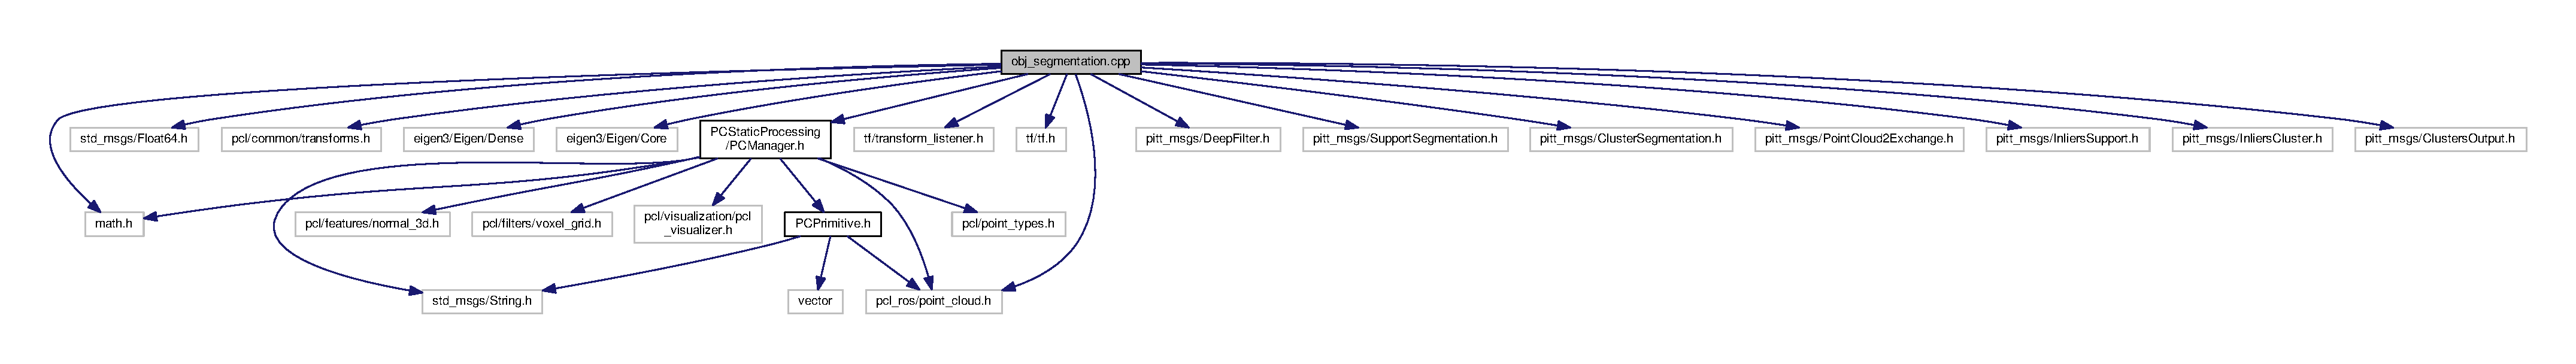
\includegraphics[width=350pt]{obj__segmentation_8cpp__incl}
\end{center}
\end{figure}
\subsection*{Typedefs}
\begin{DoxyCompactItemize}
\item 
typedef boost\-::shared\-\_\-ptr\\*
$<$ vector$<$ Inliers\-Support $>$ $>$ \hyperlink{obj__segmentation_8cpp_a054bac00065b63f36aa32247e351d7ca}{Inlier\-Supports\-Ptr}
\item 
typedef vector$<$ Inliers\-Support $>$ \hyperlink{obj__segmentation_8cpp_a7cf3ca88f8336b253d0f1080039d83dd}{Inlier\-Supports}
\item 
typedef boost\-::shared\-\_\-ptr\\*
$<$ vector$<$ Inliers\-Cluster $>$ $>$ \hyperlink{obj__segmentation_8cpp_a8f4c38bb82a38d13ea44bb3c66816597}{Inlier\-Cluster\-Ptr}
\item 
typedef vector$<$ Inliers\-Cluster $>$ \hyperlink{obj__segmentation_8cpp_a7abe79d0733f39c4aa0c917a5af115ae}{Inlier\-Clusters}
\end{DoxyCompactItemize}
\subsection*{Functions}
\begin{DoxyCompactItemize}
\item 
bool \hyperlink{obj__segmentation_8cpp_af07806e44f4c8e8e053c64eeee54dca2}{call\-Deep\-Filter} (\hyperlink{PCPrimitive_8h_aa14a240c8d999c4f56133c0f70e88783}{P\-C\-L\-Cloud\-Ptr} \&cloud)
\item 
bool \hyperlink{obj__segmentation_8cpp_a3bba1d36e0ba20c917da78be7258a8ae}{call\-Arm\-Filter} (\hyperlink{PCPrimitive_8h_aa14a240c8d999c4f56133c0f70e88783}{P\-C\-L\-Cloud\-Ptr} \&cloud)
\item 
\hyperlink{obj__segmentation_8cpp_a054bac00065b63f36aa32247e351d7ca}{Inlier\-Supports\-Ptr} \hyperlink{obj__segmentation_8cpp_a7eb9ce1c694ace5adb8e94f09e54cdae}{call\-Support\-Filter} (\hyperlink{PCPrimitive_8h_aa14a240c8d999c4f56133c0f70e88783}{P\-C\-L\-Cloud\-Ptr} input\-Cloud, \hyperlink{PCPrimitive_8h_a1bc38ce8b0c26e5f2d28fae9f3e3ea97}{P\-C\-L\-Normal\-Ptr} normal)
\item 
\hyperlink{obj__segmentation_8cpp_a8f4c38bb82a38d13ea44bb3c66816597}{Inlier\-Cluster\-Ptr} \hyperlink{obj__segmentation_8cpp_a35f42b33ad39e60ed879678fd116fa5b}{call\-Cluster\-Segmentation} (\hyperlink{PCPrimitive_8h_aa14a240c8d999c4f56133c0f70e88783}{P\-C\-L\-Cloud\-Ptr} cloud)
\item 
void \hyperlink{obj__segmentation_8cpp_a7ca1432a337f4c73ea801c2acb2de273}{log\-Avarage\-Centroid} (Inliers\-Cluster cluster\-Object)
\item 
void \hyperlink{obj__segmentation_8cpp_a480da8a5bc48bba4ac0cd49cfa4e5e7a}{depth\-Acquisition} (const Point\-Cloud2\-Ptr \&input)
\item 
int \hyperlink{obj__segmentation_8cpp_a3c04138a5bfe5d72780bb7e82a18e627}{main} (int argc, char $\ast$$\ast$argv)
\end{DoxyCompactItemize}
\subsection*{Variables}
\begin{DoxyCompactItemize}
\item 
bool \hyperlink{obj__segmentation_8cpp_aa7d893271a6dbf65066f130889d04178}{S\-H\-O\-W\-\_\-\-O\-R\-I\-G\-I\-N\-A\-L\-\_\-\-C\-L\-O\-U\-D} = false
\item 
bool \hyperlink{obj__segmentation_8cpp_a1e4cac65fffb2859d5a7d8b38fbf552c}{S\-H\-O\-W\-\_\-\-S\-U\-P\-P\-O\-R\-T\-S} = false
\item 
bool \hyperlink{obj__segmentation_8cpp_a5bf3800c59a0ba9c3a6c13fba7780c12}{S\-H\-O\-W\-\_\-\-O\-B\-J\-E\-C\-T\-\_\-\-O\-N\-\_\-\-S\-U\-P\-P\-O\-R\-T} = false
\item 
bool \hyperlink{obj__segmentation_8cpp_a5935cf1c7156fc70215625ead0dff04d}{S\-H\-O\-W\-\_\-\-C\-L\-U\-S\-T\-E\-R\-S} = true
\item 
static const int \hyperlink{obj__segmentation_8cpp_a3fea3689c92e1b2fcebd3eeafee94a5e}{M\-I\-N\-\_\-\-P\-O\-I\-N\-T\-\_\-\-I\-N\-\_\-\-O\-R\-I\-G\-I\-N\-A\-L\-\_\-\-C\-L\-O\-U\-D} = 100
\item 
static const float \hyperlink{obj__segmentation_8cpp_ae9ebb86dd14cd0fcf3bfe2dae452abb2}{D\-E\-E\-P\-T\-H\-\_\-\-T\-H\-R\-E\-S\-H\-O\-U\-L\-D} = 1.\-3f
\item 
static const float \hyperlink{obj__segmentation_8cpp_af8b66843d91c073a7339d97da05e4cfa}{M\-I\-N\-\_\-\-I\-T\-E\-R\-A\-T\-I\-V\-E\-\_\-\-C\-L\-O\-U\-D\-\_\-\-P\-E\-R\-C\-E\-N\-T\-U\-A\-L\-\_\-\-S\-I\-Z\-E} = P\-C\-Manager\-::\-D\-E\-F\-A\-U\-L\-T\-\_\-\-S\-E\-R\-V\-I\-C\-E\-\_\-\-P\-A\-R\-A\-M\-E\-T\-E\-R\-\_\-\-R\-E\-Q\-U\-E\-S\-T
\item 
static const float \hyperlink{obj__segmentation_8cpp_a1cb5f58d4341fb0ea8be5786e76e850c}{M\-I\-N\-\_\-\-P\-L\-A\-N\-E\-\_\-\-P\-E\-R\-C\-E\-N\-T\-A\-G\-E\-\_\-\-S\-I\-Z\-E} = P\-C\-Manager\-::\-D\-E\-F\-A\-U\-L\-T\-\_\-\-S\-E\-R\-V\-I\-C\-E\-\_\-\-P\-A\-R\-A\-M\-E\-T\-E\-R\-\_\-\-R\-E\-Q\-U\-E\-S\-T
\item 
static const float \hyperlink{obj__segmentation_8cpp_a31976c93f57ecffe05dcdb46e5a1eb4a}{M\-A\-X\-\_\-\-V\-A\-R\-I\-A\-N\-C\-E\-\_\-\-T\-H\-\_\-\-F\-O\-R\-\_\-\-H\-O\-R\-I\-Z\-O\-N\-T\-A\-L} = P\-C\-Manager\-::\-D\-E\-F\-A\-U\-L\-T\-\_\-\-S\-E\-R\-V\-I\-C\-E\-\_\-\-P\-A\-R\-A\-M\-E\-T\-E\-R\-\_\-\-R\-E\-Q\-U\-E\-S\-T
\item 
static const int \hyperlink{obj__segmentation_8cpp_acc65cc4496947189ecf64074b20c9a6b}{R\-A\-N\-S\-A\-C\-\_\-\-M\-A\-X\-\_\-\-I\-T\-E\-R\-A\-T\-I\-O\-N\-\_\-\-T\-H} = P\-C\-Manager\-::\-D\-E\-F\-A\-U\-L\-T\-\_\-\-S\-E\-R\-V\-I\-C\-E\-\_\-\-P\-A\-R\-A\-M\-E\-T\-E\-R\-\_\-\-R\-E\-Q\-U\-E\-S\-T
\item 
static const float \hyperlink{obj__segmentation_8cpp_ab8a45d894e93cb97afbd56586a97172d}{R\-A\-N\-S\-A\-C\-\_\-\-T\-H\-\_\-\-D\-I\-S\-T\-A\-N\-C\-E\-\_\-\-P\-O\-I\-N\-T\-\_\-\-S\-H\-A\-P\-E} = P\-C\-Manager\-::\-D\-E\-F\-A\-U\-L\-T\-\_\-\-S\-E\-R\-V\-I\-C\-E\-\_\-\-P\-A\-R\-A\-M\-E\-T\-E\-R\-\_\-\-R\-E\-Q\-U\-E\-S\-T
\item 
static const float \hyperlink{obj__segmentation_8cpp_a9dc99e81f4ba41b83214b0d6b629dd10}{R\-A\-N\-S\-A\-C\-\_\-\-N\-O\-R\-M\-A\-L\-\_\-\-D\-I\-S\-T\-A\-N\-C\-E\-\_\-\-W\-E\-I\-G\-H\-T} = P\-C\-Manager\-::\-D\-E\-F\-A\-U\-L\-T\-\_\-\-S\-E\-R\-V\-I\-C\-E\-\_\-\-P\-A\-R\-A\-M\-E\-T\-E\-R\-\_\-\-R\-E\-Q\-U\-E\-S\-T
\item 
static float \hyperlink{obj__segmentation_8cpp_a36bfa270ef95104222ed1f76120adb35}{H\-O\-R\-I\-Z\-O\-N\-T\-A\-L\-\_\-\-A\-X\-I\-S} \mbox{[}1\mbox{]} = \{ P\-C\-Manager\-::\-D\-E\-F\-A\-U\-L\-T\-\_\-\-S\-E\-R\-V\-I\-C\-E\-\_\-\-P\-A\-R\-A\-M\-E\-T\-E\-R\-\_\-\-R\-E\-Q\-U\-E\-S\-T\}
\item 
static const float \hyperlink{obj__segmentation_8cpp_a644469188b1812f4c524c642a878eff2}{T\-A\-B\-L\-E\-\_\-\-E\-D\-G\-E\-\_\-\-O\-F\-S\-E\-T} = P\-C\-Manager\-::\-D\-E\-F\-A\-U\-L\-T\-\_\-\-S\-E\-R\-V\-I\-C\-E\-\_\-\-P\-A\-R\-A\-M\-E\-T\-E\-R\-\_\-\-R\-E\-Q\-U\-E\-S\-T
\item 
static const float \hyperlink{obj__segmentation_8cpp_a88860f27251204bde59ab6495172c7b5}{C\-L\-U\-S\-T\-E\-R\-\_\-\-T\-O\-L\-L\-E\-R\-A\-N\-C\-E} = P\-C\-Manager\-::\-D\-E\-F\-A\-U\-L\-T\-\_\-\-S\-E\-R\-V\-I\-C\-E\-\_\-\-P\-A\-R\-A\-M\-E\-T\-E\-R\-\_\-\-R\-E\-Q\-U\-E\-S\-T
\item 
static const float \hyperlink{obj__segmentation_8cpp_ad88a6dc7a57d82d3ffa7a564bd27f48f}{M\-A\-X\-\_\-\-C\-L\-U\-S\-T\-E\-R\-\_\-\-S\-I\-Z\-E\-\_\-\-R\-A\-T\-E} = P\-C\-Manager\-::\-D\-E\-F\-A\-U\-L\-T\-\_\-\-S\-E\-R\-V\-I\-C\-E\-\_\-\-P\-A\-R\-A\-M\-E\-T\-E\-R\-\_\-\-R\-E\-Q\-U\-E\-S\-T
\item 
static const float \hyperlink{obj__segmentation_8cpp_afca123f0460442873968893574d6d202}{M\-I\-N\-\_\-\-C\-L\-U\-S\-T\-E\-R\-\_\-\-S\-I\-Z\-E\-\_\-\-R\-A\-T\-E} = P\-C\-Manager\-::\-D\-E\-F\-A\-U\-L\-T\-\_\-\-S\-E\-R\-V\-I\-C\-E\-\_\-\-P\-A\-R\-A\-M\-E\-T\-E\-R\-\_\-\-R\-E\-Q\-U\-E\-S\-T
\item 
static const float \hyperlink{obj__segmentation_8cpp_a4705f500e23482459d16a6992c07fd91}{M\-I\-N\-\_\-\-C\-L\-U\-S\-T\-E\-R\-\_\-\-I\-N\-P\-U\-T\-\_\-\-S\-I\-Z\-E} = P\-C\-Manager\-::\-D\-E\-F\-A\-U\-L\-T\-\_\-\-S\-E\-R\-V\-I\-C\-E\-\_\-\-P\-A\-R\-A\-M\-E\-T\-E\-R\-\_\-\-R\-E\-Q\-U\-E\-S\-T
\item 
\hyperlink{classpcm_1_1PCManager}{pcm\-::\-P\-C\-Manager} $\ast$ \hyperlink{obj__segmentation_8cpp_a21221f555fa05f2c3f45ff5592a25197}{manager} = new \hyperlink{classpcm_1_1PCManager}{pcm\-::\-P\-C\-Manager}( false)
\item 
boost\-::shared\-\_\-ptr\\*
$<$ \hyperlink{PCManager_8h_a38c805dbc7ad6f06109b85c8e540817a}{visualization\-::\-P\-C\-L\-Visualizer} $>$ \hyperlink{obj__segmentation_8cpp_a6c2d87234fca8dcca11f888098558986}{vis}
\item 
Publisher \hyperlink{obj__segmentation_8cpp_a27c3ab807dd4360a5b35f9b4813ac85c}{cluster\-Pub}
\item 
float \hyperlink{obj__segmentation_8cpp_a43fa09b9ac966a338a97687ecb22d988}{avarage\-Centroid\-\_\-\-X} = 0
\item 
float \hyperlink{obj__segmentation_8cpp_a9392d825da1c779fac248a00c7d1e746}{avarage\-Centroid\-\_\-\-Y} = 0
\item 
float \hyperlink{obj__segmentation_8cpp_a18600a5c6669c0158971be4cbe358375}{avarage\-Centroid\-\_\-\-Z} = 0
\item 
int \hyperlink{obj__segmentation_8cpp_a2d150e2c81676518e1b4a1d52dc96939}{scan\-Count} = 0
\item 
Eigen\-::\-Matrix4f \hyperlink{obj__segmentation_8cpp_abeb91134d7b10cc7475f7fa946e66a34}{pcl\-Transform}
\item 
static string \hyperlink{obj__segmentation_8cpp_a89794ef3f62d4bfa2dba13649e279e58}{centroid\-File\-Log}
\end{DoxyCompactItemize}


\subsection{Typedef Documentation}
\hypertarget{obj__segmentation_8cpp_a8f4c38bb82a38d13ea44bb3c66816597}{\index{obj\-\_\-segmentation.\-cpp@{obj\-\_\-segmentation.\-cpp}!Inlier\-Cluster\-Ptr@{Inlier\-Cluster\-Ptr}}
\index{Inlier\-Cluster\-Ptr@{Inlier\-Cluster\-Ptr}!obj_segmentation.cpp@{obj\-\_\-segmentation.\-cpp}}
\subsubsection[{Inlier\-Cluster\-Ptr}]{\setlength{\rightskip}{0pt plus 5cm}typedef boost\-::shared\-\_\-ptr$<$ vector$<$ Inliers\-Cluster$>$ $>$ {\bf Inlier\-Cluster\-Ptr}}}\label{obj__segmentation_8cpp_a8f4c38bb82a38d13ea44bb3c66816597}


Definition at line 32 of file obj\-\_\-segmentation.\-cpp.

\hypertarget{obj__segmentation_8cpp_a7abe79d0733f39c4aa0c917a5af115ae}{\index{obj\-\_\-segmentation.\-cpp@{obj\-\_\-segmentation.\-cpp}!Inlier\-Clusters@{Inlier\-Clusters}}
\index{Inlier\-Clusters@{Inlier\-Clusters}!obj_segmentation.cpp@{obj\-\_\-segmentation.\-cpp}}
\subsubsection[{Inlier\-Clusters}]{\setlength{\rightskip}{0pt plus 5cm}typedef vector$<$ Inliers\-Cluster$>$ {\bf Inlier\-Clusters}}}\label{obj__segmentation_8cpp_a7abe79d0733f39c4aa0c917a5af115ae}


Definition at line 33 of file obj\-\_\-segmentation.\-cpp.

\hypertarget{obj__segmentation_8cpp_a7cf3ca88f8336b253d0f1080039d83dd}{\index{obj\-\_\-segmentation.\-cpp@{obj\-\_\-segmentation.\-cpp}!Inlier\-Supports@{Inlier\-Supports}}
\index{Inlier\-Supports@{Inlier\-Supports}!obj_segmentation.cpp@{obj\-\_\-segmentation.\-cpp}}
\subsubsection[{Inlier\-Supports}]{\setlength{\rightskip}{0pt plus 5cm}typedef vector$<$ Inliers\-Support$>$ {\bf Inlier\-Supports}}}\label{obj__segmentation_8cpp_a7cf3ca88f8336b253d0f1080039d83dd}


Definition at line 31 of file obj\-\_\-segmentation.\-cpp.

\hypertarget{obj__segmentation_8cpp_a054bac00065b63f36aa32247e351d7ca}{\index{obj\-\_\-segmentation.\-cpp@{obj\-\_\-segmentation.\-cpp}!Inlier\-Supports\-Ptr@{Inlier\-Supports\-Ptr}}
\index{Inlier\-Supports\-Ptr@{Inlier\-Supports\-Ptr}!obj_segmentation.cpp@{obj\-\_\-segmentation.\-cpp}}
\subsubsection[{Inlier\-Supports\-Ptr}]{\setlength{\rightskip}{0pt plus 5cm}typedef boost\-::shared\-\_\-ptr$<$ vector$<$ Inliers\-Support$>$ $>$ {\bf Inlier\-Supports\-Ptr}}}\label{obj__segmentation_8cpp_a054bac00065b63f36aa32247e351d7ca}


Definition at line 30 of file obj\-\_\-segmentation.\-cpp.



\subsection{Function Documentation}
\hypertarget{obj__segmentation_8cpp_a3bba1d36e0ba20c917da78be7258a8ae}{\index{obj\-\_\-segmentation.\-cpp@{obj\-\_\-segmentation.\-cpp}!call\-Arm\-Filter@{call\-Arm\-Filter}}
\index{call\-Arm\-Filter@{call\-Arm\-Filter}!obj_segmentation.cpp@{obj\-\_\-segmentation.\-cpp}}
\subsubsection[{call\-Arm\-Filter}]{\setlength{\rightskip}{0pt plus 5cm}bool call\-Arm\-Filter (
\begin{DoxyParamCaption}
\item[{{\bf P\-C\-L\-Cloud\-Ptr} \&}]{cloud}
\end{DoxyParamCaption}
)}}\label{obj__segmentation_8cpp_a3bba1d36e0ba20c917da78be7258a8ae}


Definition at line 93 of file obj\-\_\-segmentation.\-cpp.



Referenced by depth\-Acquisition().

\hypertarget{obj__segmentation_8cpp_a35f42b33ad39e60ed879678fd116fa5b}{\index{obj\-\_\-segmentation.\-cpp@{obj\-\_\-segmentation.\-cpp}!call\-Cluster\-Segmentation@{call\-Cluster\-Segmentation}}
\index{call\-Cluster\-Segmentation@{call\-Cluster\-Segmentation}!obj_segmentation.cpp@{obj\-\_\-segmentation.\-cpp}}
\subsubsection[{call\-Cluster\-Segmentation}]{\setlength{\rightskip}{0pt plus 5cm}{\bf Inlier\-Cluster\-Ptr} call\-Cluster\-Segmentation (
\begin{DoxyParamCaption}
\item[{{\bf P\-C\-L\-Cloud\-Ptr}}]{cloud}
\end{DoxyParamCaption}
)}}\label{obj__segmentation_8cpp_a35f42b33ad39e60ed879678fd116fa5b}


Definition at line 147 of file obj\-\_\-segmentation.\-cpp.



References C\-L\-U\-S\-T\-E\-R\-\_\-\-T\-O\-L\-L\-E\-R\-A\-N\-C\-E, M\-A\-X\-\_\-\-C\-L\-U\-S\-T\-E\-R\-\_\-\-S\-I\-Z\-E\-\_\-\-R\-A\-T\-E, M\-I\-N\-\_\-\-C\-L\-U\-S\-T\-E\-R\-\_\-\-I\-N\-P\-U\-T\-\_\-\-S\-I\-Z\-E, and M\-I\-N\-\_\-\-C\-L\-U\-S\-T\-E\-R\-\_\-\-S\-I\-Z\-E\-\_\-\-R\-A\-T\-E.



Referenced by depth\-Acquisition().

\hypertarget{obj__segmentation_8cpp_af07806e44f4c8e8e053c64eeee54dca2}{\index{obj\-\_\-segmentation.\-cpp@{obj\-\_\-segmentation.\-cpp}!call\-Deep\-Filter@{call\-Deep\-Filter}}
\index{call\-Deep\-Filter@{call\-Deep\-Filter}!obj_segmentation.cpp@{obj\-\_\-segmentation.\-cpp}}
\subsubsection[{call\-Deep\-Filter}]{\setlength{\rightskip}{0pt plus 5cm}bool call\-Deep\-Filter (
\begin{DoxyParamCaption}
\item[{{\bf P\-C\-L\-Cloud\-Ptr} \&}]{cloud}
\end{DoxyParamCaption}
)}}\label{obj__segmentation_8cpp_af07806e44f4c8e8e053c64eeee54dca2}


Definition at line 67 of file obj\-\_\-segmentation.\-cpp.



References D\-E\-E\-P\-T\-H\-\_\-\-T\-H\-R\-E\-S\-H\-O\-U\-L\-D.



Referenced by depth\-Acquisition().

\hypertarget{obj__segmentation_8cpp_a7eb9ce1c694ace5adb8e94f09e54cdae}{\index{obj\-\_\-segmentation.\-cpp@{obj\-\_\-segmentation.\-cpp}!call\-Support\-Filter@{call\-Support\-Filter}}
\index{call\-Support\-Filter@{call\-Support\-Filter}!obj_segmentation.cpp@{obj\-\_\-segmentation.\-cpp}}
\subsubsection[{call\-Support\-Filter}]{\setlength{\rightskip}{0pt plus 5cm}{\bf Inlier\-Supports\-Ptr} call\-Support\-Filter (
\begin{DoxyParamCaption}
\item[{{\bf P\-C\-L\-Cloud\-Ptr}}]{input\-Cloud, }
\item[{{\bf P\-C\-L\-Normal\-Ptr}}]{normal}
\end{DoxyParamCaption}
)}}\label{obj__segmentation_8cpp_a7eb9ce1c694ace5adb8e94f09e54cdae}


Definition at line 111 of file obj\-\_\-segmentation.\-cpp.



References H\-O\-R\-I\-Z\-O\-N\-T\-A\-L\-\_\-\-A\-X\-I\-S, M\-A\-X\-\_\-\-V\-A\-R\-I\-A\-N\-C\-E\-\_\-\-T\-H\-\_\-\-F\-O\-R\-\_\-\-H\-O\-R\-I\-Z\-O\-N\-T\-A\-L, M\-I\-N\-\_\-\-I\-T\-E\-R\-A\-T\-I\-V\-E\-\_\-\-C\-L\-O\-U\-D\-\_\-\-P\-E\-R\-C\-E\-N\-T\-U\-A\-L\-\_\-\-S\-I\-Z\-E, M\-I\-N\-\_\-\-P\-L\-A\-N\-E\-\_\-\-P\-E\-R\-C\-E\-N\-T\-A\-G\-E\-\_\-\-S\-I\-Z\-E, R\-A\-N\-S\-A\-C\-\_\-\-M\-A\-X\-\_\-\-I\-T\-E\-R\-A\-T\-I\-O\-N\-\_\-\-T\-H, R\-A\-N\-S\-A\-C\-\_\-\-N\-O\-R\-M\-A\-L\-\_\-\-D\-I\-S\-T\-A\-N\-C\-E\-\_\-\-W\-E\-I\-G\-H\-T, R\-A\-N\-S\-A\-C\-\_\-\-T\-H\-\_\-\-D\-I\-S\-T\-A\-N\-C\-E\-\_\-\-P\-O\-I\-N\-T\-\_\-\-S\-H\-A\-P\-E, and T\-A\-B\-L\-E\-\_\-\-E\-D\-G\-E\-\_\-\-O\-F\-S\-E\-T.



Referenced by depth\-Acquisition().

\hypertarget{obj__segmentation_8cpp_a480da8a5bc48bba4ac0cd49cfa4e5e7a}{\index{obj\-\_\-segmentation.\-cpp@{obj\-\_\-segmentation.\-cpp}!depth\-Acquisition@{depth\-Acquisition}}
\index{depth\-Acquisition@{depth\-Acquisition}!obj_segmentation.cpp@{obj\-\_\-segmentation.\-cpp}}
\subsubsection[{depth\-Acquisition}]{\setlength{\rightskip}{0pt plus 5cm}void depth\-Acquisition (
\begin{DoxyParamCaption}
\item[{const Point\-Cloud2\-Ptr \&}]{input}
\end{DoxyParamCaption}
)}}\label{obj__segmentation_8cpp_a480da8a5bc48bba4ac0cd49cfa4e5e7a}


Definition at line 185 of file obj\-\_\-segmentation.\-cpp.



References call\-Arm\-Filter(), call\-Cluster\-Segmentation(), call\-Deep\-Filter(), call\-Support\-Filter(), centroid\-File\-Log, cluster\-Pub, M\-I\-N\-\_\-\-P\-O\-I\-N\-T\-\_\-\-I\-N\-\_\-\-O\-R\-I\-G\-I\-N\-A\-L\-\_\-\-C\-L\-O\-U\-D, pcl\-Transform, S\-H\-O\-W\-\_\-\-C\-L\-U\-S\-T\-E\-R\-S, S\-H\-O\-W\-\_\-\-O\-B\-J\-E\-C\-T\-\_\-\-O\-N\-\_\-\-S\-U\-P\-P\-O\-R\-T, S\-H\-O\-W\-\_\-\-O\-R\-I\-G\-I\-N\-A\-L\-\_\-\-C\-L\-O\-U\-D, S\-H\-O\-W\-\_\-\-S\-U\-P\-P\-O\-R\-T\-S, and vis.



Referenced by main().



Here is the call graph for this function\-:\nopagebreak
\begin{figure}[H]
\begin{center}
\leavevmode
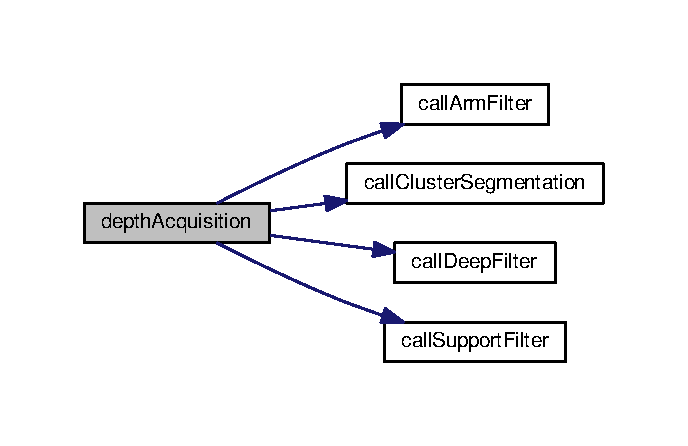
\includegraphics[width=330pt]{obj__segmentation_8cpp_a480da8a5bc48bba4ac0cd49cfa4e5e7a_cgraph}
\end{center}
\end{figure}


\hypertarget{obj__segmentation_8cpp_a7ca1432a337f4c73ea801c2acb2de273}{\index{obj\-\_\-segmentation.\-cpp@{obj\-\_\-segmentation.\-cpp}!log\-Avarage\-Centroid@{log\-Avarage\-Centroid}}
\index{log\-Avarage\-Centroid@{log\-Avarage\-Centroid}!obj_segmentation.cpp@{obj\-\_\-segmentation.\-cpp}}
\subsubsection[{log\-Avarage\-Centroid}]{\setlength{\rightskip}{0pt plus 5cm}void log\-Avarage\-Centroid (
\begin{DoxyParamCaption}
\item[{Inliers\-Cluster}]{cluster\-Object}
\end{DoxyParamCaption}
)}}\label{obj__segmentation_8cpp_a7ca1432a337f4c73ea801c2acb2de273}


Definition at line 173 of file obj\-\_\-segmentation.\-cpp.



References avarage\-Centroid\-\_\-\-X, avarage\-Centroid\-\_\-\-Y, avarage\-Centroid\-\_\-\-Z, and scan\-Count.

\hypertarget{obj__segmentation_8cpp_a3c04138a5bfe5d72780bb7e82a18e627}{\index{obj\-\_\-segmentation.\-cpp@{obj\-\_\-segmentation.\-cpp}!main@{main}}
\index{main@{main}!obj_segmentation.cpp@{obj\-\_\-segmentation.\-cpp}}
\subsubsection[{main}]{\setlength{\rightskip}{0pt plus 5cm}int main (
\begin{DoxyParamCaption}
\item[{int}]{argc, }
\item[{char $\ast$$\ast$}]{argv}
\end{DoxyParamCaption}
)}}\label{obj__segmentation_8cpp_a3c04138a5bfe5d72780bb7e82a18e627}
A\-A\-A\-A\-A


\begin{DoxyParams}{Parameters}
{\em argc} & \\
\hline
{\em argv} & \\
\hline
\end{DoxyParams}
\begin{DoxyReturn}{Returns}

\end{DoxyReturn}


Definition at line 280 of file obj\-\_\-segmentation.\-cpp.



References centroid\-File\-Log, cluster\-Pub, depth\-Acquisition(), pcl\-Transform, S\-H\-O\-W\-\_\-\-C\-L\-U\-S\-T\-E\-R\-S, S\-H\-O\-W\-\_\-\-O\-B\-J\-E\-C\-T\-\_\-\-O\-N\-\_\-\-S\-U\-P\-P\-O\-R\-T, S\-H\-O\-W\-\_\-\-O\-R\-I\-G\-I\-N\-A\-L\-\_\-\-C\-L\-O\-U\-D, S\-H\-O\-W\-\_\-\-S\-U\-P\-P\-O\-R\-T\-S, and vis.



Here is the call graph for this function\-:\nopagebreak
\begin{figure}[H]
\begin{center}
\leavevmode
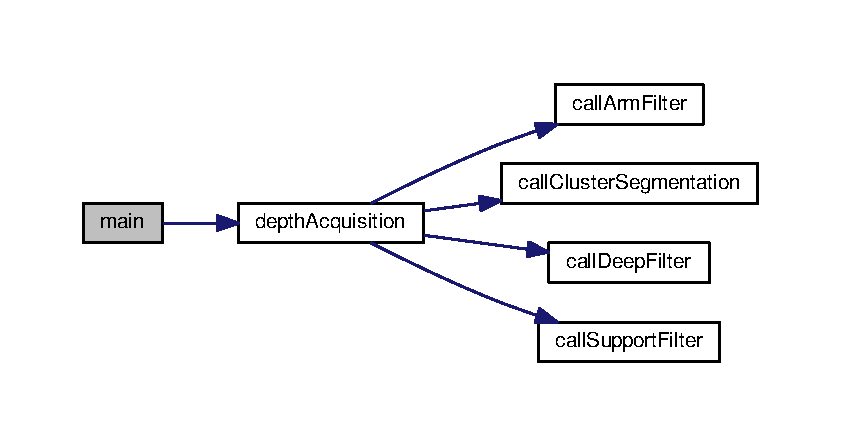
\includegraphics[width=350pt]{obj__segmentation_8cpp_a3c04138a5bfe5d72780bb7e82a18e627_cgraph}
\end{center}
\end{figure}




\subsection{Variable Documentation}
\hypertarget{obj__segmentation_8cpp_a43fa09b9ac966a338a97687ecb22d988}{\index{obj\-\_\-segmentation.\-cpp@{obj\-\_\-segmentation.\-cpp}!avarage\-Centroid\-\_\-\-X@{avarage\-Centroid\-\_\-\-X}}
\index{avarage\-Centroid\-\_\-\-X@{avarage\-Centroid\-\_\-\-X}!obj_segmentation.cpp@{obj\-\_\-segmentation.\-cpp}}
\subsubsection[{avarage\-Centroid\-\_\-\-X}]{\setlength{\rightskip}{0pt plus 5cm}float avarage\-Centroid\-\_\-\-X = 0}}\label{obj__segmentation_8cpp_a43fa09b9ac966a338a97687ecb22d988}


Definition at line 171 of file obj\-\_\-segmentation.\-cpp.



Referenced by log\-Avarage\-Centroid().

\hypertarget{obj__segmentation_8cpp_a9392d825da1c779fac248a00c7d1e746}{\index{obj\-\_\-segmentation.\-cpp@{obj\-\_\-segmentation.\-cpp}!avarage\-Centroid\-\_\-\-Y@{avarage\-Centroid\-\_\-\-Y}}
\index{avarage\-Centroid\-\_\-\-Y@{avarage\-Centroid\-\_\-\-Y}!obj_segmentation.cpp@{obj\-\_\-segmentation.\-cpp}}
\subsubsection[{avarage\-Centroid\-\_\-\-Y}]{\setlength{\rightskip}{0pt plus 5cm}float avarage\-Centroid\-\_\-\-Y = 0}}\label{obj__segmentation_8cpp_a9392d825da1c779fac248a00c7d1e746}


Definition at line 171 of file obj\-\_\-segmentation.\-cpp.



Referenced by log\-Avarage\-Centroid().

\hypertarget{obj__segmentation_8cpp_a18600a5c6669c0158971be4cbe358375}{\index{obj\-\_\-segmentation.\-cpp@{obj\-\_\-segmentation.\-cpp}!avarage\-Centroid\-\_\-\-Z@{avarage\-Centroid\-\_\-\-Z}}
\index{avarage\-Centroid\-\_\-\-Z@{avarage\-Centroid\-\_\-\-Z}!obj_segmentation.cpp@{obj\-\_\-segmentation.\-cpp}}
\subsubsection[{avarage\-Centroid\-\_\-\-Z}]{\setlength{\rightskip}{0pt plus 5cm}float avarage\-Centroid\-\_\-\-Z = 0}}\label{obj__segmentation_8cpp_a18600a5c6669c0158971be4cbe358375}


Definition at line 171 of file obj\-\_\-segmentation.\-cpp.



Referenced by log\-Avarage\-Centroid().

\hypertarget{obj__segmentation_8cpp_a89794ef3f62d4bfa2dba13649e279e58}{\index{obj\-\_\-segmentation.\-cpp@{obj\-\_\-segmentation.\-cpp}!centroid\-File\-Log@{centroid\-File\-Log}}
\index{centroid\-File\-Log@{centroid\-File\-Log}!obj_segmentation.cpp@{obj\-\_\-segmentation.\-cpp}}
\subsubsection[{centroid\-File\-Log}]{\setlength{\rightskip}{0pt plus 5cm}string centroid\-File\-Log\hspace{0.3cm}{\ttfamily [static]}}}\label{obj__segmentation_8cpp_a89794ef3f62d4bfa2dba13649e279e58}


Definition at line 184 of file obj\-\_\-segmentation.\-cpp.



Referenced by depth\-Acquisition(), and main().

\hypertarget{obj__segmentation_8cpp_a88860f27251204bde59ab6495172c7b5}{\index{obj\-\_\-segmentation.\-cpp@{obj\-\_\-segmentation.\-cpp}!C\-L\-U\-S\-T\-E\-R\-\_\-\-T\-O\-L\-L\-E\-R\-A\-N\-C\-E@{C\-L\-U\-S\-T\-E\-R\-\_\-\-T\-O\-L\-L\-E\-R\-A\-N\-C\-E}}
\index{C\-L\-U\-S\-T\-E\-R\-\_\-\-T\-O\-L\-L\-E\-R\-A\-N\-C\-E@{C\-L\-U\-S\-T\-E\-R\-\_\-\-T\-O\-L\-L\-E\-R\-A\-N\-C\-E}!obj_segmentation.cpp@{obj\-\_\-segmentation.\-cpp}}
\subsubsection[{C\-L\-U\-S\-T\-E\-R\-\_\-\-T\-O\-L\-L\-E\-R\-A\-N\-C\-E}]{\setlength{\rightskip}{0pt plus 5cm}const float C\-L\-U\-S\-T\-E\-R\-\_\-\-T\-O\-L\-L\-E\-R\-A\-N\-C\-E = P\-C\-Manager\-::\-D\-E\-F\-A\-U\-L\-T\-\_\-\-S\-E\-R\-V\-I\-C\-E\-\_\-\-P\-A\-R\-A\-M\-E\-T\-E\-R\-\_\-\-R\-E\-Q\-U\-E\-S\-T\hspace{0.3cm}{\ttfamily [static]}}}\label{obj__segmentation_8cpp_a88860f27251204bde59ab6495172c7b5}


Definition at line 55 of file obj\-\_\-segmentation.\-cpp.



Referenced by call\-Cluster\-Segmentation().

\hypertarget{obj__segmentation_8cpp_a27c3ab807dd4360a5b35f9b4813ac85c}{\index{obj\-\_\-segmentation.\-cpp@{obj\-\_\-segmentation.\-cpp}!cluster\-Pub@{cluster\-Pub}}
\index{cluster\-Pub@{cluster\-Pub}!obj_segmentation.cpp@{obj\-\_\-segmentation.\-cpp}}
\subsubsection[{cluster\-Pub}]{\setlength{\rightskip}{0pt plus 5cm}Publisher cluster\-Pub}}\label{obj__segmentation_8cpp_a27c3ab807dd4360a5b35f9b4813ac85c}


Definition at line 63 of file obj\-\_\-segmentation.\-cpp.



Referenced by depth\-Acquisition(), and main().

\hypertarget{obj__segmentation_8cpp_ae9ebb86dd14cd0fcf3bfe2dae452abb2}{\index{obj\-\_\-segmentation.\-cpp@{obj\-\_\-segmentation.\-cpp}!D\-E\-E\-P\-T\-H\-\_\-\-T\-H\-R\-E\-S\-H\-O\-U\-L\-D@{D\-E\-E\-P\-T\-H\-\_\-\-T\-H\-R\-E\-S\-H\-O\-U\-L\-D}}
\index{D\-E\-E\-P\-T\-H\-\_\-\-T\-H\-R\-E\-S\-H\-O\-U\-L\-D@{D\-E\-E\-P\-T\-H\-\_\-\-T\-H\-R\-E\-S\-H\-O\-U\-L\-D}!obj_segmentation.cpp@{obj\-\_\-segmentation.\-cpp}}
\subsubsection[{D\-E\-E\-P\-T\-H\-\_\-\-T\-H\-R\-E\-S\-H\-O\-U\-L\-D}]{\setlength{\rightskip}{0pt plus 5cm}const float D\-E\-E\-P\-T\-H\-\_\-\-T\-H\-R\-E\-S\-H\-O\-U\-L\-D = 1.\-3f\hspace{0.3cm}{\ttfamily [static]}}}\label{obj__segmentation_8cpp_ae9ebb86dd14cd0fcf3bfe2dae452abb2}


Definition at line 44 of file obj\-\_\-segmentation.\-cpp.



Referenced by call\-Deep\-Filter().

\hypertarget{obj__segmentation_8cpp_a36bfa270ef95104222ed1f76120adb35}{\index{obj\-\_\-segmentation.\-cpp@{obj\-\_\-segmentation.\-cpp}!H\-O\-R\-I\-Z\-O\-N\-T\-A\-L\-\_\-\-A\-X\-I\-S@{H\-O\-R\-I\-Z\-O\-N\-T\-A\-L\-\_\-\-A\-X\-I\-S}}
\index{H\-O\-R\-I\-Z\-O\-N\-T\-A\-L\-\_\-\-A\-X\-I\-S@{H\-O\-R\-I\-Z\-O\-N\-T\-A\-L\-\_\-\-A\-X\-I\-S}!obj_segmentation.cpp@{obj\-\_\-segmentation.\-cpp}}
\subsubsection[{H\-O\-R\-I\-Z\-O\-N\-T\-A\-L\-\_\-\-A\-X\-I\-S}]{\setlength{\rightskip}{0pt plus 5cm}float H\-O\-R\-I\-Z\-O\-N\-T\-A\-L\-\_\-\-A\-X\-I\-S\mbox{[}1\mbox{]} = \{ P\-C\-Manager\-::\-D\-E\-F\-A\-U\-L\-T\-\_\-\-S\-E\-R\-V\-I\-C\-E\-\_\-\-P\-A\-R\-A\-M\-E\-T\-E\-R\-\_\-\-R\-E\-Q\-U\-E\-S\-T\}\hspace{0.3cm}{\ttfamily [static]}}}\label{obj__segmentation_8cpp_a36bfa270ef95104222ed1f76120adb35}


Definition at line 52 of file obj\-\_\-segmentation.\-cpp.



Referenced by call\-Support\-Filter().

\hypertarget{obj__segmentation_8cpp_a21221f555fa05f2c3f45ff5592a25197}{\index{obj\-\_\-segmentation.\-cpp@{obj\-\_\-segmentation.\-cpp}!manager@{manager}}
\index{manager@{manager}!obj_segmentation.cpp@{obj\-\_\-segmentation.\-cpp}}
\subsubsection[{manager}]{\setlength{\rightskip}{0pt plus 5cm}{\bf pcm\-::\-P\-C\-Manager}$\ast$ manager = new {\bf pcm\-::\-P\-C\-Manager}( false)}}\label{obj__segmentation_8cpp_a21221f555fa05f2c3f45ff5592a25197}


Definition at line 61 of file obj\-\_\-segmentation.\-cpp.

\hypertarget{obj__segmentation_8cpp_ad88a6dc7a57d82d3ffa7a564bd27f48f}{\index{obj\-\_\-segmentation.\-cpp@{obj\-\_\-segmentation.\-cpp}!M\-A\-X\-\_\-\-C\-L\-U\-S\-T\-E\-R\-\_\-\-S\-I\-Z\-E\-\_\-\-R\-A\-T\-E@{M\-A\-X\-\_\-\-C\-L\-U\-S\-T\-E\-R\-\_\-\-S\-I\-Z\-E\-\_\-\-R\-A\-T\-E}}
\index{M\-A\-X\-\_\-\-C\-L\-U\-S\-T\-E\-R\-\_\-\-S\-I\-Z\-E\-\_\-\-R\-A\-T\-E@{M\-A\-X\-\_\-\-C\-L\-U\-S\-T\-E\-R\-\_\-\-S\-I\-Z\-E\-\_\-\-R\-A\-T\-E}!obj_segmentation.cpp@{obj\-\_\-segmentation.\-cpp}}
\subsubsection[{M\-A\-X\-\_\-\-C\-L\-U\-S\-T\-E\-R\-\_\-\-S\-I\-Z\-E\-\_\-\-R\-A\-T\-E}]{\setlength{\rightskip}{0pt plus 5cm}const float M\-A\-X\-\_\-\-C\-L\-U\-S\-T\-E\-R\-\_\-\-S\-I\-Z\-E\-\_\-\-R\-A\-T\-E = P\-C\-Manager\-::\-D\-E\-F\-A\-U\-L\-T\-\_\-\-S\-E\-R\-V\-I\-C\-E\-\_\-\-P\-A\-R\-A\-M\-E\-T\-E\-R\-\_\-\-R\-E\-Q\-U\-E\-S\-T\hspace{0.3cm}{\ttfamily [static]}}}\label{obj__segmentation_8cpp_ad88a6dc7a57d82d3ffa7a564bd27f48f}


Definition at line 56 of file obj\-\_\-segmentation.\-cpp.



Referenced by call\-Cluster\-Segmentation().

\hypertarget{obj__segmentation_8cpp_a31976c93f57ecffe05dcdb46e5a1eb4a}{\index{obj\-\_\-segmentation.\-cpp@{obj\-\_\-segmentation.\-cpp}!M\-A\-X\-\_\-\-V\-A\-R\-I\-A\-N\-C\-E\-\_\-\-T\-H\-\_\-\-F\-O\-R\-\_\-\-H\-O\-R\-I\-Z\-O\-N\-T\-A\-L@{M\-A\-X\-\_\-\-V\-A\-R\-I\-A\-N\-C\-E\-\_\-\-T\-H\-\_\-\-F\-O\-R\-\_\-\-H\-O\-R\-I\-Z\-O\-N\-T\-A\-L}}
\index{M\-A\-X\-\_\-\-V\-A\-R\-I\-A\-N\-C\-E\-\_\-\-T\-H\-\_\-\-F\-O\-R\-\_\-\-H\-O\-R\-I\-Z\-O\-N\-T\-A\-L@{M\-A\-X\-\_\-\-V\-A\-R\-I\-A\-N\-C\-E\-\_\-\-T\-H\-\_\-\-F\-O\-R\-\_\-\-H\-O\-R\-I\-Z\-O\-N\-T\-A\-L}!obj_segmentation.cpp@{obj\-\_\-segmentation.\-cpp}}
\subsubsection[{M\-A\-X\-\_\-\-V\-A\-R\-I\-A\-N\-C\-E\-\_\-\-T\-H\-\_\-\-F\-O\-R\-\_\-\-H\-O\-R\-I\-Z\-O\-N\-T\-A\-L}]{\setlength{\rightskip}{0pt plus 5cm}const float M\-A\-X\-\_\-\-V\-A\-R\-I\-A\-N\-C\-E\-\_\-\-T\-H\-\_\-\-F\-O\-R\-\_\-\-H\-O\-R\-I\-Z\-O\-N\-T\-A\-L = P\-C\-Manager\-::\-D\-E\-F\-A\-U\-L\-T\-\_\-\-S\-E\-R\-V\-I\-C\-E\-\_\-\-P\-A\-R\-A\-M\-E\-T\-E\-R\-\_\-\-R\-E\-Q\-U\-E\-S\-T\hspace{0.3cm}{\ttfamily [static]}}}\label{obj__segmentation_8cpp_a31976c93f57ecffe05dcdb46e5a1eb4a}


Definition at line 48 of file obj\-\_\-segmentation.\-cpp.



Referenced by call\-Support\-Filter().

\hypertarget{obj__segmentation_8cpp_a4705f500e23482459d16a6992c07fd91}{\index{obj\-\_\-segmentation.\-cpp@{obj\-\_\-segmentation.\-cpp}!M\-I\-N\-\_\-\-C\-L\-U\-S\-T\-E\-R\-\_\-\-I\-N\-P\-U\-T\-\_\-\-S\-I\-Z\-E@{M\-I\-N\-\_\-\-C\-L\-U\-S\-T\-E\-R\-\_\-\-I\-N\-P\-U\-T\-\_\-\-S\-I\-Z\-E}}
\index{M\-I\-N\-\_\-\-C\-L\-U\-S\-T\-E\-R\-\_\-\-I\-N\-P\-U\-T\-\_\-\-S\-I\-Z\-E@{M\-I\-N\-\_\-\-C\-L\-U\-S\-T\-E\-R\-\_\-\-I\-N\-P\-U\-T\-\_\-\-S\-I\-Z\-E}!obj_segmentation.cpp@{obj\-\_\-segmentation.\-cpp}}
\subsubsection[{M\-I\-N\-\_\-\-C\-L\-U\-S\-T\-E\-R\-\_\-\-I\-N\-P\-U\-T\-\_\-\-S\-I\-Z\-E}]{\setlength{\rightskip}{0pt plus 5cm}const float M\-I\-N\-\_\-\-C\-L\-U\-S\-T\-E\-R\-\_\-\-I\-N\-P\-U\-T\-\_\-\-S\-I\-Z\-E = P\-C\-Manager\-::\-D\-E\-F\-A\-U\-L\-T\-\_\-\-S\-E\-R\-V\-I\-C\-E\-\_\-\-P\-A\-R\-A\-M\-E\-T\-E\-R\-\_\-\-R\-E\-Q\-U\-E\-S\-T\hspace{0.3cm}{\ttfamily [static]}}}\label{obj__segmentation_8cpp_a4705f500e23482459d16a6992c07fd91}


Definition at line 58 of file obj\-\_\-segmentation.\-cpp.



Referenced by call\-Cluster\-Segmentation().

\hypertarget{obj__segmentation_8cpp_afca123f0460442873968893574d6d202}{\index{obj\-\_\-segmentation.\-cpp@{obj\-\_\-segmentation.\-cpp}!M\-I\-N\-\_\-\-C\-L\-U\-S\-T\-E\-R\-\_\-\-S\-I\-Z\-E\-\_\-\-R\-A\-T\-E@{M\-I\-N\-\_\-\-C\-L\-U\-S\-T\-E\-R\-\_\-\-S\-I\-Z\-E\-\_\-\-R\-A\-T\-E}}
\index{M\-I\-N\-\_\-\-C\-L\-U\-S\-T\-E\-R\-\_\-\-S\-I\-Z\-E\-\_\-\-R\-A\-T\-E@{M\-I\-N\-\_\-\-C\-L\-U\-S\-T\-E\-R\-\_\-\-S\-I\-Z\-E\-\_\-\-R\-A\-T\-E}!obj_segmentation.cpp@{obj\-\_\-segmentation.\-cpp}}
\subsubsection[{M\-I\-N\-\_\-\-C\-L\-U\-S\-T\-E\-R\-\_\-\-S\-I\-Z\-E\-\_\-\-R\-A\-T\-E}]{\setlength{\rightskip}{0pt plus 5cm}const float M\-I\-N\-\_\-\-C\-L\-U\-S\-T\-E\-R\-\_\-\-S\-I\-Z\-E\-\_\-\-R\-A\-T\-E = P\-C\-Manager\-::\-D\-E\-F\-A\-U\-L\-T\-\_\-\-S\-E\-R\-V\-I\-C\-E\-\_\-\-P\-A\-R\-A\-M\-E\-T\-E\-R\-\_\-\-R\-E\-Q\-U\-E\-S\-T\hspace{0.3cm}{\ttfamily [static]}}}\label{obj__segmentation_8cpp_afca123f0460442873968893574d6d202}


Definition at line 57 of file obj\-\_\-segmentation.\-cpp.



Referenced by call\-Cluster\-Segmentation().

\hypertarget{obj__segmentation_8cpp_af8b66843d91c073a7339d97da05e4cfa}{\index{obj\-\_\-segmentation.\-cpp@{obj\-\_\-segmentation.\-cpp}!M\-I\-N\-\_\-\-I\-T\-E\-R\-A\-T\-I\-V\-E\-\_\-\-C\-L\-O\-U\-D\-\_\-\-P\-E\-R\-C\-E\-N\-T\-U\-A\-L\-\_\-\-S\-I\-Z\-E@{M\-I\-N\-\_\-\-I\-T\-E\-R\-A\-T\-I\-V\-E\-\_\-\-C\-L\-O\-U\-D\-\_\-\-P\-E\-R\-C\-E\-N\-T\-U\-A\-L\-\_\-\-S\-I\-Z\-E}}
\index{M\-I\-N\-\_\-\-I\-T\-E\-R\-A\-T\-I\-V\-E\-\_\-\-C\-L\-O\-U\-D\-\_\-\-P\-E\-R\-C\-E\-N\-T\-U\-A\-L\-\_\-\-S\-I\-Z\-E@{M\-I\-N\-\_\-\-I\-T\-E\-R\-A\-T\-I\-V\-E\-\_\-\-C\-L\-O\-U\-D\-\_\-\-P\-E\-R\-C\-E\-N\-T\-U\-A\-L\-\_\-\-S\-I\-Z\-E}!obj_segmentation.cpp@{obj\-\_\-segmentation.\-cpp}}
\subsubsection[{M\-I\-N\-\_\-\-I\-T\-E\-R\-A\-T\-I\-V\-E\-\_\-\-C\-L\-O\-U\-D\-\_\-\-P\-E\-R\-C\-E\-N\-T\-U\-A\-L\-\_\-\-S\-I\-Z\-E}]{\setlength{\rightskip}{0pt plus 5cm}const float M\-I\-N\-\_\-\-I\-T\-E\-R\-A\-T\-I\-V\-E\-\_\-\-C\-L\-O\-U\-D\-\_\-\-P\-E\-R\-C\-E\-N\-T\-U\-A\-L\-\_\-\-S\-I\-Z\-E = P\-C\-Manager\-::\-D\-E\-F\-A\-U\-L\-T\-\_\-\-S\-E\-R\-V\-I\-C\-E\-\_\-\-P\-A\-R\-A\-M\-E\-T\-E\-R\-\_\-\-R\-E\-Q\-U\-E\-S\-T\hspace{0.3cm}{\ttfamily [static]}}}\label{obj__segmentation_8cpp_af8b66843d91c073a7339d97da05e4cfa}


Definition at line 46 of file obj\-\_\-segmentation.\-cpp.



Referenced by call\-Support\-Filter().

\hypertarget{obj__segmentation_8cpp_a1cb5f58d4341fb0ea8be5786e76e850c}{\index{obj\-\_\-segmentation.\-cpp@{obj\-\_\-segmentation.\-cpp}!M\-I\-N\-\_\-\-P\-L\-A\-N\-E\-\_\-\-P\-E\-R\-C\-E\-N\-T\-A\-G\-E\-\_\-\-S\-I\-Z\-E@{M\-I\-N\-\_\-\-P\-L\-A\-N\-E\-\_\-\-P\-E\-R\-C\-E\-N\-T\-A\-G\-E\-\_\-\-S\-I\-Z\-E}}
\index{M\-I\-N\-\_\-\-P\-L\-A\-N\-E\-\_\-\-P\-E\-R\-C\-E\-N\-T\-A\-G\-E\-\_\-\-S\-I\-Z\-E@{M\-I\-N\-\_\-\-P\-L\-A\-N\-E\-\_\-\-P\-E\-R\-C\-E\-N\-T\-A\-G\-E\-\_\-\-S\-I\-Z\-E}!obj_segmentation.cpp@{obj\-\_\-segmentation.\-cpp}}
\subsubsection[{M\-I\-N\-\_\-\-P\-L\-A\-N\-E\-\_\-\-P\-E\-R\-C\-E\-N\-T\-A\-G\-E\-\_\-\-S\-I\-Z\-E}]{\setlength{\rightskip}{0pt plus 5cm}const float M\-I\-N\-\_\-\-P\-L\-A\-N\-E\-\_\-\-P\-E\-R\-C\-E\-N\-T\-A\-G\-E\-\_\-\-S\-I\-Z\-E = P\-C\-Manager\-::\-D\-E\-F\-A\-U\-L\-T\-\_\-\-S\-E\-R\-V\-I\-C\-E\-\_\-\-P\-A\-R\-A\-M\-E\-T\-E\-R\-\_\-\-R\-E\-Q\-U\-E\-S\-T\hspace{0.3cm}{\ttfamily [static]}}}\label{obj__segmentation_8cpp_a1cb5f58d4341fb0ea8be5786e76e850c}


Definition at line 47 of file obj\-\_\-segmentation.\-cpp.



Referenced by call\-Support\-Filter().

\hypertarget{obj__segmentation_8cpp_a3fea3689c92e1b2fcebd3eeafee94a5e}{\index{obj\-\_\-segmentation.\-cpp@{obj\-\_\-segmentation.\-cpp}!M\-I\-N\-\_\-\-P\-O\-I\-N\-T\-\_\-\-I\-N\-\_\-\-O\-R\-I\-G\-I\-N\-A\-L\-\_\-\-C\-L\-O\-U\-D@{M\-I\-N\-\_\-\-P\-O\-I\-N\-T\-\_\-\-I\-N\-\_\-\-O\-R\-I\-G\-I\-N\-A\-L\-\_\-\-C\-L\-O\-U\-D}}
\index{M\-I\-N\-\_\-\-P\-O\-I\-N\-T\-\_\-\-I\-N\-\_\-\-O\-R\-I\-G\-I\-N\-A\-L\-\_\-\-C\-L\-O\-U\-D@{M\-I\-N\-\_\-\-P\-O\-I\-N\-T\-\_\-\-I\-N\-\_\-\-O\-R\-I\-G\-I\-N\-A\-L\-\_\-\-C\-L\-O\-U\-D}!obj_segmentation.cpp@{obj\-\_\-segmentation.\-cpp}}
\subsubsection[{M\-I\-N\-\_\-\-P\-O\-I\-N\-T\-\_\-\-I\-N\-\_\-\-O\-R\-I\-G\-I\-N\-A\-L\-\_\-\-C\-L\-O\-U\-D}]{\setlength{\rightskip}{0pt plus 5cm}const int M\-I\-N\-\_\-\-P\-O\-I\-N\-T\-\_\-\-I\-N\-\_\-\-O\-R\-I\-G\-I\-N\-A\-L\-\_\-\-C\-L\-O\-U\-D = 100\hspace{0.3cm}{\ttfamily [static]}}}\label{obj__segmentation_8cpp_a3fea3689c92e1b2fcebd3eeafee94a5e}


Definition at line 42 of file obj\-\_\-segmentation.\-cpp.



Referenced by depth\-Acquisition().

\hypertarget{obj__segmentation_8cpp_abeb91134d7b10cc7475f7fa946e66a34}{\index{obj\-\_\-segmentation.\-cpp@{obj\-\_\-segmentation.\-cpp}!pcl\-Transform@{pcl\-Transform}}
\index{pcl\-Transform@{pcl\-Transform}!obj_segmentation.cpp@{obj\-\_\-segmentation.\-cpp}}
\subsubsection[{pcl\-Transform}]{\setlength{\rightskip}{0pt plus 5cm}Eigen\-::\-Matrix4f pcl\-Transform}}\label{obj__segmentation_8cpp_abeb91134d7b10cc7475f7fa946e66a34}


Definition at line 183 of file obj\-\_\-segmentation.\-cpp.



Referenced by depth\-Acquisition(), and main().

\hypertarget{obj__segmentation_8cpp_acc65cc4496947189ecf64074b20c9a6b}{\index{obj\-\_\-segmentation.\-cpp@{obj\-\_\-segmentation.\-cpp}!R\-A\-N\-S\-A\-C\-\_\-\-M\-A\-X\-\_\-\-I\-T\-E\-R\-A\-T\-I\-O\-N\-\_\-\-T\-H@{R\-A\-N\-S\-A\-C\-\_\-\-M\-A\-X\-\_\-\-I\-T\-E\-R\-A\-T\-I\-O\-N\-\_\-\-T\-H}}
\index{R\-A\-N\-S\-A\-C\-\_\-\-M\-A\-X\-\_\-\-I\-T\-E\-R\-A\-T\-I\-O\-N\-\_\-\-T\-H@{R\-A\-N\-S\-A\-C\-\_\-\-M\-A\-X\-\_\-\-I\-T\-E\-R\-A\-T\-I\-O\-N\-\_\-\-T\-H}!obj_segmentation.cpp@{obj\-\_\-segmentation.\-cpp}}
\subsubsection[{R\-A\-N\-S\-A\-C\-\_\-\-M\-A\-X\-\_\-\-I\-T\-E\-R\-A\-T\-I\-O\-N\-\_\-\-T\-H}]{\setlength{\rightskip}{0pt plus 5cm}const int R\-A\-N\-S\-A\-C\-\_\-\-M\-A\-X\-\_\-\-I\-T\-E\-R\-A\-T\-I\-O\-N\-\_\-\-T\-H = P\-C\-Manager\-::\-D\-E\-F\-A\-U\-L\-T\-\_\-\-S\-E\-R\-V\-I\-C\-E\-\_\-\-P\-A\-R\-A\-M\-E\-T\-E\-R\-\_\-\-R\-E\-Q\-U\-E\-S\-T\hspace{0.3cm}{\ttfamily [static]}}}\label{obj__segmentation_8cpp_acc65cc4496947189ecf64074b20c9a6b}


Definition at line 49 of file obj\-\_\-segmentation.\-cpp.



Referenced by call\-Support\-Filter().

\hypertarget{obj__segmentation_8cpp_a9dc99e81f4ba41b83214b0d6b629dd10}{\index{obj\-\_\-segmentation.\-cpp@{obj\-\_\-segmentation.\-cpp}!R\-A\-N\-S\-A\-C\-\_\-\-N\-O\-R\-M\-A\-L\-\_\-\-D\-I\-S\-T\-A\-N\-C\-E\-\_\-\-W\-E\-I\-G\-H\-T@{R\-A\-N\-S\-A\-C\-\_\-\-N\-O\-R\-M\-A\-L\-\_\-\-D\-I\-S\-T\-A\-N\-C\-E\-\_\-\-W\-E\-I\-G\-H\-T}}
\index{R\-A\-N\-S\-A\-C\-\_\-\-N\-O\-R\-M\-A\-L\-\_\-\-D\-I\-S\-T\-A\-N\-C\-E\-\_\-\-W\-E\-I\-G\-H\-T@{R\-A\-N\-S\-A\-C\-\_\-\-N\-O\-R\-M\-A\-L\-\_\-\-D\-I\-S\-T\-A\-N\-C\-E\-\_\-\-W\-E\-I\-G\-H\-T}!obj_segmentation.cpp@{obj\-\_\-segmentation.\-cpp}}
\subsubsection[{R\-A\-N\-S\-A\-C\-\_\-\-N\-O\-R\-M\-A\-L\-\_\-\-D\-I\-S\-T\-A\-N\-C\-E\-\_\-\-W\-E\-I\-G\-H\-T}]{\setlength{\rightskip}{0pt plus 5cm}const float R\-A\-N\-S\-A\-C\-\_\-\-N\-O\-R\-M\-A\-L\-\_\-\-D\-I\-S\-T\-A\-N\-C\-E\-\_\-\-W\-E\-I\-G\-H\-T = P\-C\-Manager\-::\-D\-E\-F\-A\-U\-L\-T\-\_\-\-S\-E\-R\-V\-I\-C\-E\-\_\-\-P\-A\-R\-A\-M\-E\-T\-E\-R\-\_\-\-R\-E\-Q\-U\-E\-S\-T\hspace{0.3cm}{\ttfamily [static]}}}\label{obj__segmentation_8cpp_a9dc99e81f4ba41b83214b0d6b629dd10}


Definition at line 51 of file obj\-\_\-segmentation.\-cpp.



Referenced by call\-Support\-Filter().

\hypertarget{obj__segmentation_8cpp_ab8a45d894e93cb97afbd56586a97172d}{\index{obj\-\_\-segmentation.\-cpp@{obj\-\_\-segmentation.\-cpp}!R\-A\-N\-S\-A\-C\-\_\-\-T\-H\-\_\-\-D\-I\-S\-T\-A\-N\-C\-E\-\_\-\-P\-O\-I\-N\-T\-\_\-\-S\-H\-A\-P\-E@{R\-A\-N\-S\-A\-C\-\_\-\-T\-H\-\_\-\-D\-I\-S\-T\-A\-N\-C\-E\-\_\-\-P\-O\-I\-N\-T\-\_\-\-S\-H\-A\-P\-E}}
\index{R\-A\-N\-S\-A\-C\-\_\-\-T\-H\-\_\-\-D\-I\-S\-T\-A\-N\-C\-E\-\_\-\-P\-O\-I\-N\-T\-\_\-\-S\-H\-A\-P\-E@{R\-A\-N\-S\-A\-C\-\_\-\-T\-H\-\_\-\-D\-I\-S\-T\-A\-N\-C\-E\-\_\-\-P\-O\-I\-N\-T\-\_\-\-S\-H\-A\-P\-E}!obj_segmentation.cpp@{obj\-\_\-segmentation.\-cpp}}
\subsubsection[{R\-A\-N\-S\-A\-C\-\_\-\-T\-H\-\_\-\-D\-I\-S\-T\-A\-N\-C\-E\-\_\-\-P\-O\-I\-N\-T\-\_\-\-S\-H\-A\-P\-E}]{\setlength{\rightskip}{0pt plus 5cm}const float R\-A\-N\-S\-A\-C\-\_\-\-T\-H\-\_\-\-D\-I\-S\-T\-A\-N\-C\-E\-\_\-\-P\-O\-I\-N\-T\-\_\-\-S\-H\-A\-P\-E = P\-C\-Manager\-::\-D\-E\-F\-A\-U\-L\-T\-\_\-\-S\-E\-R\-V\-I\-C\-E\-\_\-\-P\-A\-R\-A\-M\-E\-T\-E\-R\-\_\-\-R\-E\-Q\-U\-E\-S\-T\hspace{0.3cm}{\ttfamily [static]}}}\label{obj__segmentation_8cpp_ab8a45d894e93cb97afbd56586a97172d}


Definition at line 50 of file obj\-\_\-segmentation.\-cpp.



Referenced by call\-Support\-Filter().

\hypertarget{obj__segmentation_8cpp_a2d150e2c81676518e1b4a1d52dc96939}{\index{obj\-\_\-segmentation.\-cpp@{obj\-\_\-segmentation.\-cpp}!scan\-Count@{scan\-Count}}
\index{scan\-Count@{scan\-Count}!obj_segmentation.cpp@{obj\-\_\-segmentation.\-cpp}}
\subsubsection[{scan\-Count}]{\setlength{\rightskip}{0pt plus 5cm}int scan\-Count = 0}}\label{obj__segmentation_8cpp_a2d150e2c81676518e1b4a1d52dc96939}


Definition at line 172 of file obj\-\_\-segmentation.\-cpp.



Referenced by log\-Avarage\-Centroid().

\hypertarget{obj__segmentation_8cpp_a5935cf1c7156fc70215625ead0dff04d}{\index{obj\-\_\-segmentation.\-cpp@{obj\-\_\-segmentation.\-cpp}!S\-H\-O\-W\-\_\-\-C\-L\-U\-S\-T\-E\-R\-S@{S\-H\-O\-W\-\_\-\-C\-L\-U\-S\-T\-E\-R\-S}}
\index{S\-H\-O\-W\-\_\-\-C\-L\-U\-S\-T\-E\-R\-S@{S\-H\-O\-W\-\_\-\-C\-L\-U\-S\-T\-E\-R\-S}!obj_segmentation.cpp@{obj\-\_\-segmentation.\-cpp}}
\subsubsection[{S\-H\-O\-W\-\_\-\-C\-L\-U\-S\-T\-E\-R\-S}]{\setlength{\rightskip}{0pt plus 5cm}bool S\-H\-O\-W\-\_\-\-C\-L\-U\-S\-T\-E\-R\-S = true}}\label{obj__segmentation_8cpp_a5935cf1c7156fc70215625ead0dff04d}


Definition at line 40 of file obj\-\_\-segmentation.\-cpp.



Referenced by depth\-Acquisition(), and main().

\hypertarget{obj__segmentation_8cpp_a5bf3800c59a0ba9c3a6c13fba7780c12}{\index{obj\-\_\-segmentation.\-cpp@{obj\-\_\-segmentation.\-cpp}!S\-H\-O\-W\-\_\-\-O\-B\-J\-E\-C\-T\-\_\-\-O\-N\-\_\-\-S\-U\-P\-P\-O\-R\-T@{S\-H\-O\-W\-\_\-\-O\-B\-J\-E\-C\-T\-\_\-\-O\-N\-\_\-\-S\-U\-P\-P\-O\-R\-T}}
\index{S\-H\-O\-W\-\_\-\-O\-B\-J\-E\-C\-T\-\_\-\-O\-N\-\_\-\-S\-U\-P\-P\-O\-R\-T@{S\-H\-O\-W\-\_\-\-O\-B\-J\-E\-C\-T\-\_\-\-O\-N\-\_\-\-S\-U\-P\-P\-O\-R\-T}!obj_segmentation.cpp@{obj\-\_\-segmentation.\-cpp}}
\subsubsection[{S\-H\-O\-W\-\_\-\-O\-B\-J\-E\-C\-T\-\_\-\-O\-N\-\_\-\-S\-U\-P\-P\-O\-R\-T}]{\setlength{\rightskip}{0pt plus 5cm}bool S\-H\-O\-W\-\_\-\-O\-B\-J\-E\-C\-T\-\_\-\-O\-N\-\_\-\-S\-U\-P\-P\-O\-R\-T = false}}\label{obj__segmentation_8cpp_a5bf3800c59a0ba9c3a6c13fba7780c12}


Definition at line 39 of file obj\-\_\-segmentation.\-cpp.



Referenced by depth\-Acquisition(), and main().

\hypertarget{obj__segmentation_8cpp_aa7d893271a6dbf65066f130889d04178}{\index{obj\-\_\-segmentation.\-cpp@{obj\-\_\-segmentation.\-cpp}!S\-H\-O\-W\-\_\-\-O\-R\-I\-G\-I\-N\-A\-L\-\_\-\-C\-L\-O\-U\-D@{S\-H\-O\-W\-\_\-\-O\-R\-I\-G\-I\-N\-A\-L\-\_\-\-C\-L\-O\-U\-D}}
\index{S\-H\-O\-W\-\_\-\-O\-R\-I\-G\-I\-N\-A\-L\-\_\-\-C\-L\-O\-U\-D@{S\-H\-O\-W\-\_\-\-O\-R\-I\-G\-I\-N\-A\-L\-\_\-\-C\-L\-O\-U\-D}!obj_segmentation.cpp@{obj\-\_\-segmentation.\-cpp}}
\subsubsection[{S\-H\-O\-W\-\_\-\-O\-R\-I\-G\-I\-N\-A\-L\-\_\-\-C\-L\-O\-U\-D}]{\setlength{\rightskip}{0pt plus 5cm}bool S\-H\-O\-W\-\_\-\-O\-R\-I\-G\-I\-N\-A\-L\-\_\-\-C\-L\-O\-U\-D = false}}\label{obj__segmentation_8cpp_aa7d893271a6dbf65066f130889d04178}


Definition at line 37 of file obj\-\_\-segmentation.\-cpp.



Referenced by depth\-Acquisition(), and main().

\hypertarget{obj__segmentation_8cpp_a1e4cac65fffb2859d5a7d8b38fbf552c}{\index{obj\-\_\-segmentation.\-cpp@{obj\-\_\-segmentation.\-cpp}!S\-H\-O\-W\-\_\-\-S\-U\-P\-P\-O\-R\-T\-S@{S\-H\-O\-W\-\_\-\-S\-U\-P\-P\-O\-R\-T\-S}}
\index{S\-H\-O\-W\-\_\-\-S\-U\-P\-P\-O\-R\-T\-S@{S\-H\-O\-W\-\_\-\-S\-U\-P\-P\-O\-R\-T\-S}!obj_segmentation.cpp@{obj\-\_\-segmentation.\-cpp}}
\subsubsection[{S\-H\-O\-W\-\_\-\-S\-U\-P\-P\-O\-R\-T\-S}]{\setlength{\rightskip}{0pt plus 5cm}bool S\-H\-O\-W\-\_\-\-S\-U\-P\-P\-O\-R\-T\-S = false}}\label{obj__segmentation_8cpp_a1e4cac65fffb2859d5a7d8b38fbf552c}


Definition at line 38 of file obj\-\_\-segmentation.\-cpp.



Referenced by depth\-Acquisition(), and main().

\hypertarget{obj__segmentation_8cpp_a644469188b1812f4c524c642a878eff2}{\index{obj\-\_\-segmentation.\-cpp@{obj\-\_\-segmentation.\-cpp}!T\-A\-B\-L\-E\-\_\-\-E\-D\-G\-E\-\_\-\-O\-F\-S\-E\-T@{T\-A\-B\-L\-E\-\_\-\-E\-D\-G\-E\-\_\-\-O\-F\-S\-E\-T}}
\index{T\-A\-B\-L\-E\-\_\-\-E\-D\-G\-E\-\_\-\-O\-F\-S\-E\-T@{T\-A\-B\-L\-E\-\_\-\-E\-D\-G\-E\-\_\-\-O\-F\-S\-E\-T}!obj_segmentation.cpp@{obj\-\_\-segmentation.\-cpp}}
\subsubsection[{T\-A\-B\-L\-E\-\_\-\-E\-D\-G\-E\-\_\-\-O\-F\-S\-E\-T}]{\setlength{\rightskip}{0pt plus 5cm}const float T\-A\-B\-L\-E\-\_\-\-E\-D\-G\-E\-\_\-\-O\-F\-S\-E\-T = P\-C\-Manager\-::\-D\-E\-F\-A\-U\-L\-T\-\_\-\-S\-E\-R\-V\-I\-C\-E\-\_\-\-P\-A\-R\-A\-M\-E\-T\-E\-R\-\_\-\-R\-E\-Q\-U\-E\-S\-T\hspace{0.3cm}{\ttfamily [static]}}}\label{obj__segmentation_8cpp_a644469188b1812f4c524c642a878eff2}


Definition at line 53 of file obj\-\_\-segmentation.\-cpp.



Referenced by call\-Support\-Filter().

\hypertarget{obj__segmentation_8cpp_a6c2d87234fca8dcca11f888098558986}{\index{obj\-\_\-segmentation.\-cpp@{obj\-\_\-segmentation.\-cpp}!vis@{vis}}
\index{vis@{vis}!obj_segmentation.cpp@{obj\-\_\-segmentation.\-cpp}}
\subsubsection[{vis}]{\setlength{\rightskip}{0pt plus 5cm}boost\-::shared\-\_\-ptr$<$ {\bf visualization\-::\-P\-C\-L\-Visualizer}$>$ vis}}\label{obj__segmentation_8cpp_a6c2d87234fca8dcca11f888098558986}


Definition at line 62 of file obj\-\_\-segmentation.\-cpp.



Referenced by depth\-Acquisition(), and main().


\hypertarget{pcl__arm__filter__srv_8cpp}{\section{pcl\-\_\-arm\-\_\-filter\-\_\-srv.\-cpp File Reference}
\label{pcl__arm__filter__srv_8cpp}\index{pcl\-\_\-arm\-\_\-filter\-\_\-srv.\-cpp@{pcl\-\_\-arm\-\_\-filter\-\_\-srv.\-cpp}}
}
{\ttfamily \#include $<$ros/ros.\-h$>$}\\*
{\ttfamily \#include $<$tf/transform\-\_\-listener.\-h$>$}\\*
{\ttfamily \#include $<$tf/transform\-\_\-broadcaster.\-h$>$}\\*
{\ttfamily \#include $<$sensor\-\_\-msgs/\-Point\-Cloud2.\-h$>$}\\*
{\ttfamily \#include $<$pcl\-\_\-conversions/pcl\-\_\-conversions.\-h$>$}\\*
{\ttfamily \#include $<$pcl\-\_\-ros/point\-\_\-cloud.\-h$>$}\\*
{\ttfamily \#include $<$pcl\-\_\-ros/filters/crop\-\_\-box.\-h$>$}\\*
{\ttfamily \#include $<$pitt\-\_\-msgs/\-Point\-Cloud2\-Exchange.\-h$>$}\\*
{\ttfamily \#include \char`\"{}../\-P\-C\-Static\-Processing/\-P\-C\-Manager.\-h\char`\"{}}\\*
Include dependency graph for pcl\-\_\-arm\-\_\-filter\-\_\-srv.\-cpp\-:\nopagebreak
\begin{figure}[H]
\begin{center}
\leavevmode
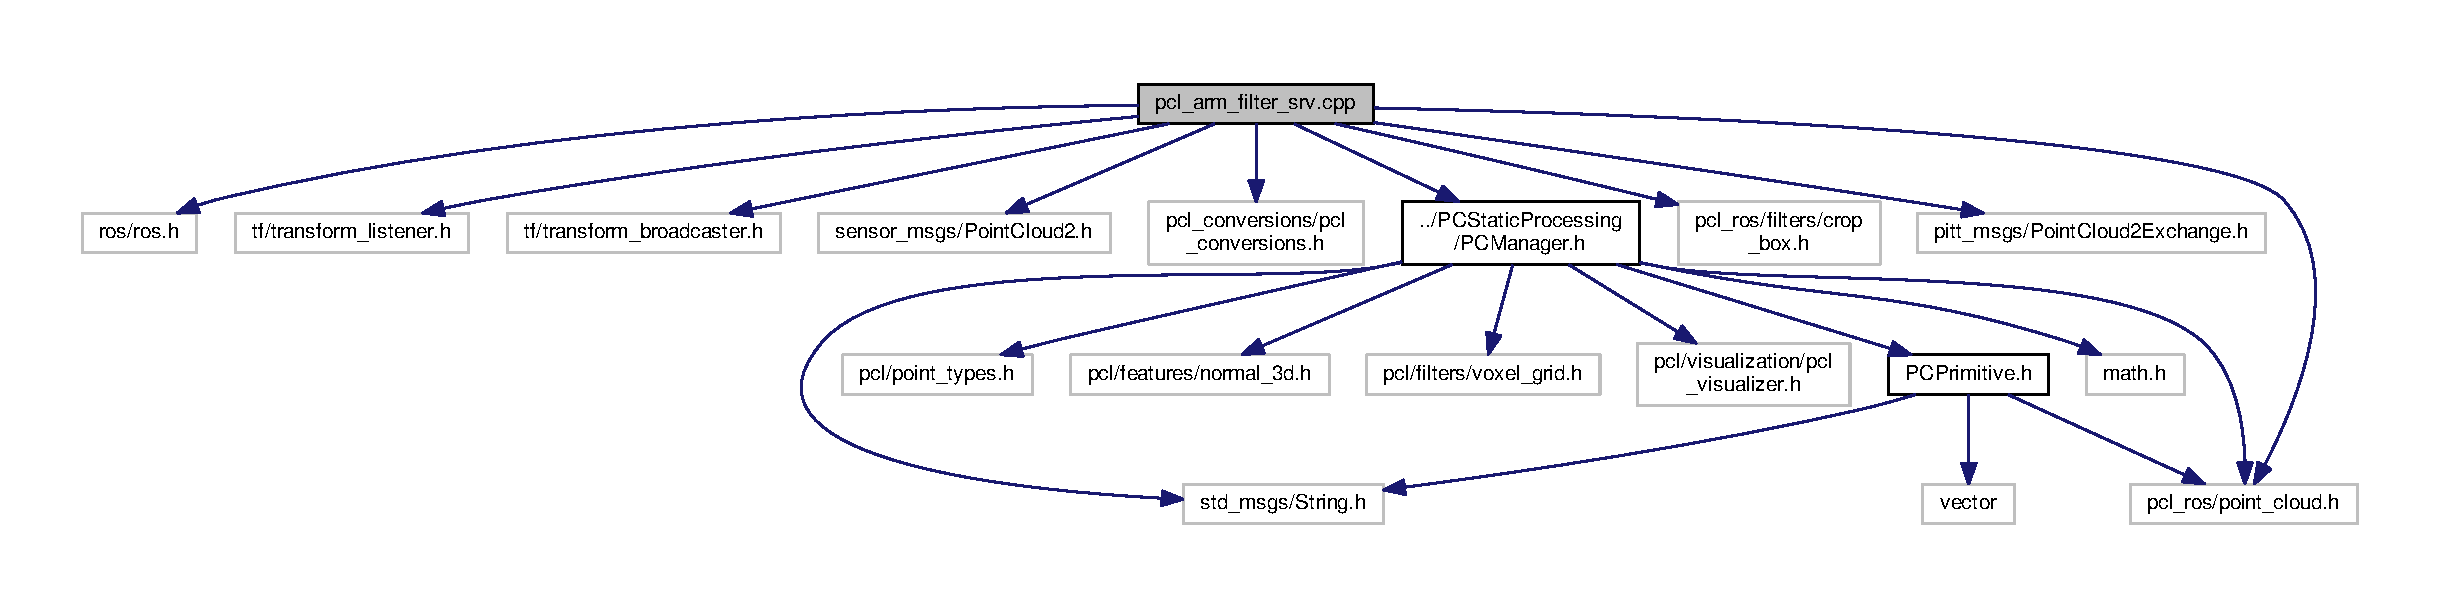
\includegraphics[width=350pt]{pcl__arm__filter__srv_8cpp__incl}
\end{center}
\end{figure}
\subsection*{Typedefs}
\begin{DoxyCompactItemize}
\item 
typedef pcl\-::\-Point\-Cloud\\*
$<$ pcl\-::\-Point\-X\-Y\-Z $>$ \hyperlink{pcl__arm__filter__srv_8cpp_a29f570b87ddde9c9a67921f43564b7d4}{P\-C\-L\-Cloud}
\item 
typedef pcl\-::\-Point\-Cloud\\*
$<$ pcl\-::\-Point\-X\-Y\-Z $>$\-::Ptr \hyperlink{pcl__arm__filter__srv_8cpp_a3088acf82e1f026966b77cf8cc8c545b}{P\-C\-L\-Cloud\-Ptr}
\end{DoxyCompactItemize}
\subsection*{Functions}
\begin{DoxyCompactItemize}
\item 
\hyperlink{PCPrimitive_8h_aa14a240c8d999c4f56133c0f70e88783}{P\-C\-L\-Cloud\-Ptr} \hyperlink{pcl__arm__filter__srv_8cpp_a4b5f9e676122ea81018e287be90c84c7}{arm\-Filtering} (\hyperlink{PCPrimitive_8h_aa14a240c8d999c4f56133c0f70e88783}{P\-C\-L\-Cloud\-Ptr} original, Eigen\-::\-Vector4f min\-Values, Eigen\-::\-Vector4f max\-Values, tf\-::\-Stamped\-Transform frame)
\item 
bool \hyperlink{pcl__arm__filter__srv_8cpp_a62d45b46a7caeab39f53ca574bb2d06f}{filter} (Point\-Cloud2\-Exchange\-Request \&input, Point\-Cloud2\-Exchange\-Response \&output)
\item 
int \hyperlink{pcl__arm__filter__srv_8cpp_a3c04138a5bfe5d72780bb7e82a18e627}{main} (int argc, char $\ast$$\ast$argv)
\end{DoxyCompactItemize}
\subsection*{Variables}
\begin{DoxyCompactItemize}
\item 
double \hyperlink{pcl__arm__filter__srv_8cpp_a1d3228afa3a1d6773954f40c1e519eb9}{roll}
\item 
double \hyperlink{pcl__arm__filter__srv_8cpp_a34c057a0378030db67bd6a129f37d938}{pitch}
\item 
double \hyperlink{pcl__arm__filter__srv_8cpp_a21cd490f6191f66678f55b4c242a10cf}{yaw}
\item 
Eigen\-::\-Vector3f \hyperlink{pcl__arm__filter__srv_8cpp_a3131a4e19d28e7b521a9a9e43c614c26}{translation}
\item 
Eigen\-::\-Vector3f \hyperlink{pcl__arm__filter__srv_8cpp_a84cf1f449714525e255aa53d26b62ecf}{rotation}
\item 
Eigen\-::\-Affine3f \hyperlink{pcl__arm__filter__srv_8cpp_a82c8dace269f9b25efa4df02f0b03c22}{trans} = Eigen\-::\-Affine3f\-::\-Identity()
\item 
Crop\-Box$<$ Point\-X\-Y\-Z $>$ \hyperlink{pcl__arm__filter__srv_8cpp_aeb82dd78a6dd9961f37215018fa75eb9}{crop\-Filter}
\item 
Eigen\-::\-Vector4f \hyperlink{pcl__arm__filter__srv_8cpp_a7f47885731f8cd105ee36bba21169d80}{forearm\-Min\-Value}
\item 
Eigen\-::\-Vector4f \hyperlink{pcl__arm__filter__srv_8cpp_ae6035812b8bac346e387528c918bf89b}{elbow\-Min\-Value}
\item 
Eigen\-::\-Vector4f \hyperlink{pcl__arm__filter__srv_8cpp_ab7ce5712ed01d5b0493fa15673b7e983}{forearm\-Max\-Value}
\item 
Eigen\-::\-Vector4f \hyperlink{pcl__arm__filter__srv_8cpp_a338077c8c5be4000bad261d71636489a}{elbow\-Max\-Value}
\item 
tf\-::\-Stamped\-Transform \hyperlink{pcl__arm__filter__srv_8cpp_a03bbdf8543233b1c12921461687df69f}{left\-\_\-lower\-\_\-forearm\-\_\-frame}
\item 
tf\-::\-Stamped\-Transform \hyperlink{pcl__arm__filter__srv_8cpp_a096616fea0057d98b09e63fdc9684613}{right\-\_\-lower\-\_\-forearm\-\_\-frame}
\item 
tf\-::\-Stamped\-Transform \hyperlink{pcl__arm__filter__srv_8cpp_ae9b406a81134a444f264cc1e13cdc22b}{left\-\_\-lower\-\_\-elbow\-\_\-frame}
\item 
tf\-::\-Stamped\-Transform \hyperlink{pcl__arm__filter__srv_8cpp_a1f57372612334e34a394bfb273c55e81}{right\-\_\-lower\-\_\-elbow\-\_\-frame}
\item 
tf\-::\-Quaternion \hyperlink{pcl__arm__filter__srv_8cpp_aacea208b467add8c9197eab918214974}{rot\-Quat}
\item 
tf\-::\-Matrix3x3 \hyperlink{pcl__arm__filter__srv_8cpp_abc3338eed95d1aec56b3049915a96aff}{rot\-Mat}
\item 
bool \hyperlink{pcl__arm__filter__srv_8cpp_a163bafbb51ee2789c7dcc991b5a1e903}{tf\-Error} = false
\end{DoxyCompactItemize}


\subsection{Typedef Documentation}
\hypertarget{pcl__arm__filter__srv_8cpp_a29f570b87ddde9c9a67921f43564b7d4}{\index{pcl\-\_\-arm\-\_\-filter\-\_\-srv.\-cpp@{pcl\-\_\-arm\-\_\-filter\-\_\-srv.\-cpp}!P\-C\-L\-Cloud@{P\-C\-L\-Cloud}}
\index{P\-C\-L\-Cloud@{P\-C\-L\-Cloud}!pcl_arm_filter_srv.cpp@{pcl\-\_\-arm\-\_\-filter\-\_\-srv.\-cpp}}
\subsubsection[{P\-C\-L\-Cloud}]{\setlength{\rightskip}{0pt plus 5cm}typedef pcl\-::\-Point\-Cloud$<$pcl\-::\-Point\-X\-Y\-Z$>$ {\bf P\-C\-L\-Cloud}}}\label{pcl__arm__filter__srv_8cpp_a29f570b87ddde9c9a67921f43564b7d4}


Definition at line 24 of file pcl\-\_\-arm\-\_\-filter\-\_\-srv.\-cpp.

\hypertarget{pcl__arm__filter__srv_8cpp_a3088acf82e1f026966b77cf8cc8c545b}{\index{pcl\-\_\-arm\-\_\-filter\-\_\-srv.\-cpp@{pcl\-\_\-arm\-\_\-filter\-\_\-srv.\-cpp}!P\-C\-L\-Cloud\-Ptr@{P\-C\-L\-Cloud\-Ptr}}
\index{P\-C\-L\-Cloud\-Ptr@{P\-C\-L\-Cloud\-Ptr}!pcl_arm_filter_srv.cpp@{pcl\-\_\-arm\-\_\-filter\-\_\-srv.\-cpp}}
\subsubsection[{P\-C\-L\-Cloud\-Ptr}]{\setlength{\rightskip}{0pt plus 5cm}typedef pcl\-::\-Point\-Cloud$<$pcl\-::\-Point\-X\-Y\-Z$>$\-::Ptr {\bf P\-C\-L\-Cloud\-Ptr}}}\label{pcl__arm__filter__srv_8cpp_a3088acf82e1f026966b77cf8cc8c545b}


Definition at line 25 of file pcl\-\_\-arm\-\_\-filter\-\_\-srv.\-cpp.



\subsection{Function Documentation}
\hypertarget{pcl__arm__filter__srv_8cpp_a4b5f9e676122ea81018e287be90c84c7}{\index{pcl\-\_\-arm\-\_\-filter\-\_\-srv.\-cpp@{pcl\-\_\-arm\-\_\-filter\-\_\-srv.\-cpp}!arm\-Filtering@{arm\-Filtering}}
\index{arm\-Filtering@{arm\-Filtering}!pcl_arm_filter_srv.cpp@{pcl\-\_\-arm\-\_\-filter\-\_\-srv.\-cpp}}
\subsubsection[{arm\-Filtering}]{\setlength{\rightskip}{0pt plus 5cm}{\bf P\-C\-L\-Cloud\-Ptr} arm\-Filtering (
\begin{DoxyParamCaption}
\item[{{\bf P\-C\-L\-Cloud\-Ptr}}]{original, }
\item[{Eigen\-::\-Vector4f}]{min\-Values, }
\item[{Eigen\-::\-Vector4f}]{max\-Values, }
\item[{tf\-::\-Stamped\-Transform}]{frame}
\end{DoxyParamCaption}
)}}\label{pcl__arm__filter__srv_8cpp_a4b5f9e676122ea81018e287be90c84c7}


Definition at line 53 of file pcl\-\_\-arm\-\_\-filter\-\_\-srv.\-cpp.



References crop\-Filter, pitch, roll, rotation, rot\-Mat, rot\-Quat, trans, translation, and yaw.



Referenced by filter().

\hypertarget{pcl__arm__filter__srv_8cpp_a62d45b46a7caeab39f53ca574bb2d06f}{\index{pcl\-\_\-arm\-\_\-filter\-\_\-srv.\-cpp@{pcl\-\_\-arm\-\_\-filter\-\_\-srv.\-cpp}!filter@{filter}}
\index{filter@{filter}!pcl_arm_filter_srv.cpp@{pcl\-\_\-arm\-\_\-filter\-\_\-srv.\-cpp}}
\subsubsection[{filter}]{\setlength{\rightskip}{0pt plus 5cm}bool filter (
\begin{DoxyParamCaption}
\item[{Point\-Cloud2\-Exchange\-Request \&}]{input, }
\item[{Point\-Cloud2\-Exchange\-Response \&}]{output}
\end{DoxyParamCaption}
)}}\label{pcl__arm__filter__srv_8cpp_a62d45b46a7caeab39f53ca574bb2d06f}


Definition at line 86 of file pcl\-\_\-arm\-\_\-filter\-\_\-srv.\-cpp.



References arm\-Filtering(), elbow\-Max\-Value, elbow\-Min\-Value, forearm\-Max\-Value, forearm\-Min\-Value, left\-\_\-lower\-\_\-elbow\-\_\-frame, left\-\_\-lower\-\_\-forearm\-\_\-frame, right\-\_\-lower\-\_\-elbow\-\_\-frame, right\-\_\-lower\-\_\-forearm\-\_\-frame, and tf\-Error.



Referenced by main().



Here is the call graph for this function\-:\nopagebreak
\begin{figure}[H]
\begin{center}
\leavevmode
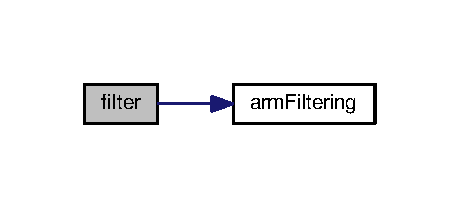
\includegraphics[width=220pt]{pcl__arm__filter__srv_8cpp_a62d45b46a7caeab39f53ca574bb2d06f_cgraph}
\end{center}
\end{figure}


\hypertarget{pcl__arm__filter__srv_8cpp_a3c04138a5bfe5d72780bb7e82a18e627}{\index{pcl\-\_\-arm\-\_\-filter\-\_\-srv.\-cpp@{pcl\-\_\-arm\-\_\-filter\-\_\-srv.\-cpp}!main@{main}}
\index{main@{main}!pcl_arm_filter_srv.cpp@{pcl\-\_\-arm\-\_\-filter\-\_\-srv.\-cpp}}
\subsubsection[{main}]{\setlength{\rightskip}{0pt plus 5cm}int main (
\begin{DoxyParamCaption}
\item[{int}]{argc, }
\item[{char $\ast$$\ast$}]{argv}
\end{DoxyParamCaption}
)}}\label{pcl__arm__filter__srv_8cpp_a3c04138a5bfe5d72780bb7e82a18e627}


Definition at line 130 of file pcl\-\_\-arm\-\_\-filter\-\_\-srv.\-cpp.



References elbow\-Max\-Value, elbow\-Min\-Value, filter(), forearm\-Max\-Value, forearm\-Min\-Value, left\-\_\-lower\-\_\-elbow\-\_\-frame, left\-\_\-lower\-\_\-forearm\-\_\-frame, right\-\_\-lower\-\_\-elbow\-\_\-frame, right\-\_\-lower\-\_\-forearm\-\_\-frame, and tf\-Error.



Here is the call graph for this function\-:\nopagebreak
\begin{figure}[H]
\begin{center}
\leavevmode
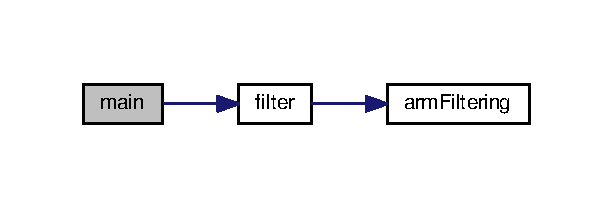
\includegraphics[width=294pt]{pcl__arm__filter__srv_8cpp_a3c04138a5bfe5d72780bb7e82a18e627_cgraph}
\end{center}
\end{figure}




\subsection{Variable Documentation}
\hypertarget{pcl__arm__filter__srv_8cpp_aeb82dd78a6dd9961f37215018fa75eb9}{\index{pcl\-\_\-arm\-\_\-filter\-\_\-srv.\-cpp@{pcl\-\_\-arm\-\_\-filter\-\_\-srv.\-cpp}!crop\-Filter@{crop\-Filter}}
\index{crop\-Filter@{crop\-Filter}!pcl_arm_filter_srv.cpp@{pcl\-\_\-arm\-\_\-filter\-\_\-srv.\-cpp}}
\subsubsection[{crop\-Filter}]{\setlength{\rightskip}{0pt plus 5cm}Crop\-Box$<$Point\-X\-Y\-Z$>$ crop\-Filter}}\label{pcl__arm__filter__srv_8cpp_aeb82dd78a6dd9961f37215018fa75eb9}


Definition at line 34 of file pcl\-\_\-arm\-\_\-filter\-\_\-srv.\-cpp.



Referenced by arm\-Filtering().

\hypertarget{pcl__arm__filter__srv_8cpp_a338077c8c5be4000bad261d71636489a}{\index{pcl\-\_\-arm\-\_\-filter\-\_\-srv.\-cpp@{pcl\-\_\-arm\-\_\-filter\-\_\-srv.\-cpp}!elbow\-Max\-Value@{elbow\-Max\-Value}}
\index{elbow\-Max\-Value@{elbow\-Max\-Value}!pcl_arm_filter_srv.cpp@{pcl\-\_\-arm\-\_\-filter\-\_\-srv.\-cpp}}
\subsubsection[{elbow\-Max\-Value}]{\setlength{\rightskip}{0pt plus 5cm}Eigen\-::\-Vector4f elbow\-Max\-Value}}\label{pcl__arm__filter__srv_8cpp_a338077c8c5be4000bad261d71636489a}


Definition at line 42 of file pcl\-\_\-arm\-\_\-filter\-\_\-srv.\-cpp.



Referenced by filter(), and main().

\hypertarget{pcl__arm__filter__srv_8cpp_ae6035812b8bac346e387528c918bf89b}{\index{pcl\-\_\-arm\-\_\-filter\-\_\-srv.\-cpp@{pcl\-\_\-arm\-\_\-filter\-\_\-srv.\-cpp}!elbow\-Min\-Value@{elbow\-Min\-Value}}
\index{elbow\-Min\-Value@{elbow\-Min\-Value}!pcl_arm_filter_srv.cpp@{pcl\-\_\-arm\-\_\-filter\-\_\-srv.\-cpp}}
\subsubsection[{elbow\-Min\-Value}]{\setlength{\rightskip}{0pt plus 5cm}Eigen\-::\-Vector4f elbow\-Min\-Value}}\label{pcl__arm__filter__srv_8cpp_ae6035812b8bac346e387528c918bf89b}


Definition at line 38 of file pcl\-\_\-arm\-\_\-filter\-\_\-srv.\-cpp.



Referenced by filter(), and main().

\hypertarget{pcl__arm__filter__srv_8cpp_ab7ce5712ed01d5b0493fa15673b7e983}{\index{pcl\-\_\-arm\-\_\-filter\-\_\-srv.\-cpp@{pcl\-\_\-arm\-\_\-filter\-\_\-srv.\-cpp}!forearm\-Max\-Value@{forearm\-Max\-Value}}
\index{forearm\-Max\-Value@{forearm\-Max\-Value}!pcl_arm_filter_srv.cpp@{pcl\-\_\-arm\-\_\-filter\-\_\-srv.\-cpp}}
\subsubsection[{forearm\-Max\-Value}]{\setlength{\rightskip}{0pt plus 5cm}Eigen\-::\-Vector4f forearm\-Max\-Value}}\label{pcl__arm__filter__srv_8cpp_ab7ce5712ed01d5b0493fa15673b7e983}


Definition at line 41 of file pcl\-\_\-arm\-\_\-filter\-\_\-srv.\-cpp.



Referenced by filter(), and main().

\hypertarget{pcl__arm__filter__srv_8cpp_a7f47885731f8cd105ee36bba21169d80}{\index{pcl\-\_\-arm\-\_\-filter\-\_\-srv.\-cpp@{pcl\-\_\-arm\-\_\-filter\-\_\-srv.\-cpp}!forearm\-Min\-Value@{forearm\-Min\-Value}}
\index{forearm\-Min\-Value@{forearm\-Min\-Value}!pcl_arm_filter_srv.cpp@{pcl\-\_\-arm\-\_\-filter\-\_\-srv.\-cpp}}
\subsubsection[{forearm\-Min\-Value}]{\setlength{\rightskip}{0pt plus 5cm}Eigen\-::\-Vector4f forearm\-Min\-Value}}\label{pcl__arm__filter__srv_8cpp_a7f47885731f8cd105ee36bba21169d80}


Definition at line 37 of file pcl\-\_\-arm\-\_\-filter\-\_\-srv.\-cpp.



Referenced by filter(), and main().

\hypertarget{pcl__arm__filter__srv_8cpp_ae9b406a81134a444f264cc1e13cdc22b}{\index{pcl\-\_\-arm\-\_\-filter\-\_\-srv.\-cpp@{pcl\-\_\-arm\-\_\-filter\-\_\-srv.\-cpp}!left\-\_\-lower\-\_\-elbow\-\_\-frame@{left\-\_\-lower\-\_\-elbow\-\_\-frame}}
\index{left\-\_\-lower\-\_\-elbow\-\_\-frame@{left\-\_\-lower\-\_\-elbow\-\_\-frame}!pcl_arm_filter_srv.cpp@{pcl\-\_\-arm\-\_\-filter\-\_\-srv.\-cpp}}
\subsubsection[{left\-\_\-lower\-\_\-elbow\-\_\-frame}]{\setlength{\rightskip}{0pt plus 5cm}tf\-::\-Stamped\-Transform left\-\_\-lower\-\_\-elbow\-\_\-frame}}\label{pcl__arm__filter__srv_8cpp_ae9b406a81134a444f264cc1e13cdc22b}


Definition at line 46 of file pcl\-\_\-arm\-\_\-filter\-\_\-srv.\-cpp.



Referenced by filter(), and main().

\hypertarget{pcl__arm__filter__srv_8cpp_a03bbdf8543233b1c12921461687df69f}{\index{pcl\-\_\-arm\-\_\-filter\-\_\-srv.\-cpp@{pcl\-\_\-arm\-\_\-filter\-\_\-srv.\-cpp}!left\-\_\-lower\-\_\-forearm\-\_\-frame@{left\-\_\-lower\-\_\-forearm\-\_\-frame}}
\index{left\-\_\-lower\-\_\-forearm\-\_\-frame@{left\-\_\-lower\-\_\-forearm\-\_\-frame}!pcl_arm_filter_srv.cpp@{pcl\-\_\-arm\-\_\-filter\-\_\-srv.\-cpp}}
\subsubsection[{left\-\_\-lower\-\_\-forearm\-\_\-frame}]{\setlength{\rightskip}{0pt plus 5cm}tf\-::\-Stamped\-Transform left\-\_\-lower\-\_\-forearm\-\_\-frame}}\label{pcl__arm__filter__srv_8cpp_a03bbdf8543233b1c12921461687df69f}


Definition at line 46 of file pcl\-\_\-arm\-\_\-filter\-\_\-srv.\-cpp.



Referenced by filter(), and main().

\hypertarget{pcl__arm__filter__srv_8cpp_a34c057a0378030db67bd6a129f37d938}{\index{pcl\-\_\-arm\-\_\-filter\-\_\-srv.\-cpp@{pcl\-\_\-arm\-\_\-filter\-\_\-srv.\-cpp}!pitch@{pitch}}
\index{pitch@{pitch}!pcl_arm_filter_srv.cpp@{pcl\-\_\-arm\-\_\-filter\-\_\-srv.\-cpp}}
\subsubsection[{pitch}]{\setlength{\rightskip}{0pt plus 5cm}double pitch}}\label{pcl__arm__filter__srv_8cpp_a34c057a0378030db67bd6a129f37d938}


Definition at line 27 of file pcl\-\_\-arm\-\_\-filter\-\_\-srv.\-cpp.



Referenced by arm\-Filtering().

\hypertarget{pcl__arm__filter__srv_8cpp_a1f57372612334e34a394bfb273c55e81}{\index{pcl\-\_\-arm\-\_\-filter\-\_\-srv.\-cpp@{pcl\-\_\-arm\-\_\-filter\-\_\-srv.\-cpp}!right\-\_\-lower\-\_\-elbow\-\_\-frame@{right\-\_\-lower\-\_\-elbow\-\_\-frame}}
\index{right\-\_\-lower\-\_\-elbow\-\_\-frame@{right\-\_\-lower\-\_\-elbow\-\_\-frame}!pcl_arm_filter_srv.cpp@{pcl\-\_\-arm\-\_\-filter\-\_\-srv.\-cpp}}
\subsubsection[{right\-\_\-lower\-\_\-elbow\-\_\-frame}]{\setlength{\rightskip}{0pt plus 5cm}tf\-::\-Stamped\-Transform right\-\_\-lower\-\_\-elbow\-\_\-frame}}\label{pcl__arm__filter__srv_8cpp_a1f57372612334e34a394bfb273c55e81}


Definition at line 46 of file pcl\-\_\-arm\-\_\-filter\-\_\-srv.\-cpp.



Referenced by filter(), and main().

\hypertarget{pcl__arm__filter__srv_8cpp_a096616fea0057d98b09e63fdc9684613}{\index{pcl\-\_\-arm\-\_\-filter\-\_\-srv.\-cpp@{pcl\-\_\-arm\-\_\-filter\-\_\-srv.\-cpp}!right\-\_\-lower\-\_\-forearm\-\_\-frame@{right\-\_\-lower\-\_\-forearm\-\_\-frame}}
\index{right\-\_\-lower\-\_\-forearm\-\_\-frame@{right\-\_\-lower\-\_\-forearm\-\_\-frame}!pcl_arm_filter_srv.cpp@{pcl\-\_\-arm\-\_\-filter\-\_\-srv.\-cpp}}
\subsubsection[{right\-\_\-lower\-\_\-forearm\-\_\-frame}]{\setlength{\rightskip}{0pt plus 5cm}tf\-::\-Stamped\-Transform right\-\_\-lower\-\_\-forearm\-\_\-frame}}\label{pcl__arm__filter__srv_8cpp_a096616fea0057d98b09e63fdc9684613}


Definition at line 46 of file pcl\-\_\-arm\-\_\-filter\-\_\-srv.\-cpp.



Referenced by filter(), and main().

\hypertarget{pcl__arm__filter__srv_8cpp_a1d3228afa3a1d6773954f40c1e519eb9}{\index{pcl\-\_\-arm\-\_\-filter\-\_\-srv.\-cpp@{pcl\-\_\-arm\-\_\-filter\-\_\-srv.\-cpp}!roll@{roll}}
\index{roll@{roll}!pcl_arm_filter_srv.cpp@{pcl\-\_\-arm\-\_\-filter\-\_\-srv.\-cpp}}
\subsubsection[{roll}]{\setlength{\rightskip}{0pt plus 5cm}double roll}}\label{pcl__arm__filter__srv_8cpp_a1d3228afa3a1d6773954f40c1e519eb9}


Definition at line 27 of file pcl\-\_\-arm\-\_\-filter\-\_\-srv.\-cpp.



Referenced by arm\-Filtering().

\hypertarget{pcl__arm__filter__srv_8cpp_a84cf1f449714525e255aa53d26b62ecf}{\index{pcl\-\_\-arm\-\_\-filter\-\_\-srv.\-cpp@{pcl\-\_\-arm\-\_\-filter\-\_\-srv.\-cpp}!rotation@{rotation}}
\index{rotation@{rotation}!pcl_arm_filter_srv.cpp@{pcl\-\_\-arm\-\_\-filter\-\_\-srv.\-cpp}}
\subsubsection[{rotation}]{\setlength{\rightskip}{0pt plus 5cm}Eigen\-::\-Vector3f rotation}}\label{pcl__arm__filter__srv_8cpp_a84cf1f449714525e255aa53d26b62ecf}


Definition at line 31 of file pcl\-\_\-arm\-\_\-filter\-\_\-srv.\-cpp.



Referenced by arm\-Filtering().

\hypertarget{pcl__arm__filter__srv_8cpp_abc3338eed95d1aec56b3049915a96aff}{\index{pcl\-\_\-arm\-\_\-filter\-\_\-srv.\-cpp@{pcl\-\_\-arm\-\_\-filter\-\_\-srv.\-cpp}!rot\-Mat@{rot\-Mat}}
\index{rot\-Mat@{rot\-Mat}!pcl_arm_filter_srv.cpp@{pcl\-\_\-arm\-\_\-filter\-\_\-srv.\-cpp}}
\subsubsection[{rot\-Mat}]{\setlength{\rightskip}{0pt plus 5cm}tf\-::\-Matrix3x3 rot\-Mat}}\label{pcl__arm__filter__srv_8cpp_abc3338eed95d1aec56b3049915a96aff}


Definition at line 48 of file pcl\-\_\-arm\-\_\-filter\-\_\-srv.\-cpp.



Referenced by arm\-Filtering().

\hypertarget{pcl__arm__filter__srv_8cpp_aacea208b467add8c9197eab918214974}{\index{pcl\-\_\-arm\-\_\-filter\-\_\-srv.\-cpp@{pcl\-\_\-arm\-\_\-filter\-\_\-srv.\-cpp}!rot\-Quat@{rot\-Quat}}
\index{rot\-Quat@{rot\-Quat}!pcl_arm_filter_srv.cpp@{pcl\-\_\-arm\-\_\-filter\-\_\-srv.\-cpp}}
\subsubsection[{rot\-Quat}]{\setlength{\rightskip}{0pt plus 5cm}tf\-::\-Quaternion rot\-Quat}}\label{pcl__arm__filter__srv_8cpp_aacea208b467add8c9197eab918214974}


Definition at line 47 of file pcl\-\_\-arm\-\_\-filter\-\_\-srv.\-cpp.



Referenced by arm\-Filtering().

\hypertarget{pcl__arm__filter__srv_8cpp_a163bafbb51ee2789c7dcc991b5a1e903}{\index{pcl\-\_\-arm\-\_\-filter\-\_\-srv.\-cpp@{pcl\-\_\-arm\-\_\-filter\-\_\-srv.\-cpp}!tf\-Error@{tf\-Error}}
\index{tf\-Error@{tf\-Error}!pcl_arm_filter_srv.cpp@{pcl\-\_\-arm\-\_\-filter\-\_\-srv.\-cpp}}
\subsubsection[{tf\-Error}]{\setlength{\rightskip}{0pt plus 5cm}bool tf\-Error = false}}\label{pcl__arm__filter__srv_8cpp_a163bafbb51ee2789c7dcc991b5a1e903}


Definition at line 49 of file pcl\-\_\-arm\-\_\-filter\-\_\-srv.\-cpp.



Referenced by filter(), and main().

\hypertarget{pcl__arm__filter__srv_8cpp_a82c8dace269f9b25efa4df02f0b03c22}{\index{pcl\-\_\-arm\-\_\-filter\-\_\-srv.\-cpp@{pcl\-\_\-arm\-\_\-filter\-\_\-srv.\-cpp}!trans@{trans}}
\index{trans@{trans}!pcl_arm_filter_srv.cpp@{pcl\-\_\-arm\-\_\-filter\-\_\-srv.\-cpp}}
\subsubsection[{trans}]{\setlength{\rightskip}{0pt plus 5cm}Eigen\-::\-Affine3f trans = Eigen\-::\-Affine3f\-::\-Identity()}}\label{pcl__arm__filter__srv_8cpp_a82c8dace269f9b25efa4df02f0b03c22}


Definition at line 32 of file pcl\-\_\-arm\-\_\-filter\-\_\-srv.\-cpp.



Referenced by arm\-Filtering().

\hypertarget{pcl__arm__filter__srv_8cpp_a3131a4e19d28e7b521a9a9e43c614c26}{\index{pcl\-\_\-arm\-\_\-filter\-\_\-srv.\-cpp@{pcl\-\_\-arm\-\_\-filter\-\_\-srv.\-cpp}!translation@{translation}}
\index{translation@{translation}!pcl_arm_filter_srv.cpp@{pcl\-\_\-arm\-\_\-filter\-\_\-srv.\-cpp}}
\subsubsection[{translation}]{\setlength{\rightskip}{0pt plus 5cm}Eigen\-::\-Vector3f translation}}\label{pcl__arm__filter__srv_8cpp_a3131a4e19d28e7b521a9a9e43c614c26}


Definition at line 30 of file pcl\-\_\-arm\-\_\-filter\-\_\-srv.\-cpp.



Referenced by arm\-Filtering().

\hypertarget{pcl__arm__filter__srv_8cpp_a21cd490f6191f66678f55b4c242a10cf}{\index{pcl\-\_\-arm\-\_\-filter\-\_\-srv.\-cpp@{pcl\-\_\-arm\-\_\-filter\-\_\-srv.\-cpp}!yaw@{yaw}}
\index{yaw@{yaw}!pcl_arm_filter_srv.cpp@{pcl\-\_\-arm\-\_\-filter\-\_\-srv.\-cpp}}
\subsubsection[{yaw}]{\setlength{\rightskip}{0pt plus 5cm}double yaw}}\label{pcl__arm__filter__srv_8cpp_a21cd490f6191f66678f55b4c242a10cf}


Definition at line 27 of file pcl\-\_\-arm\-\_\-filter\-\_\-srv.\-cpp.



Referenced by arm\-Filtering().


\hypertarget{PCManager_8cpp}{\section{P\-C\-Manager.\-cpp File Reference}
\label{PCManager_8cpp}\index{P\-C\-Manager.\-cpp@{P\-C\-Manager.\-cpp}}
}
{\ttfamily \#include \char`\"{}P\-C\-Manager.\-h\char`\"{}}\\*
Include dependency graph for P\-C\-Manager.\-cpp\-:\nopagebreak
\begin{figure}[H]
\begin{center}
\leavevmode
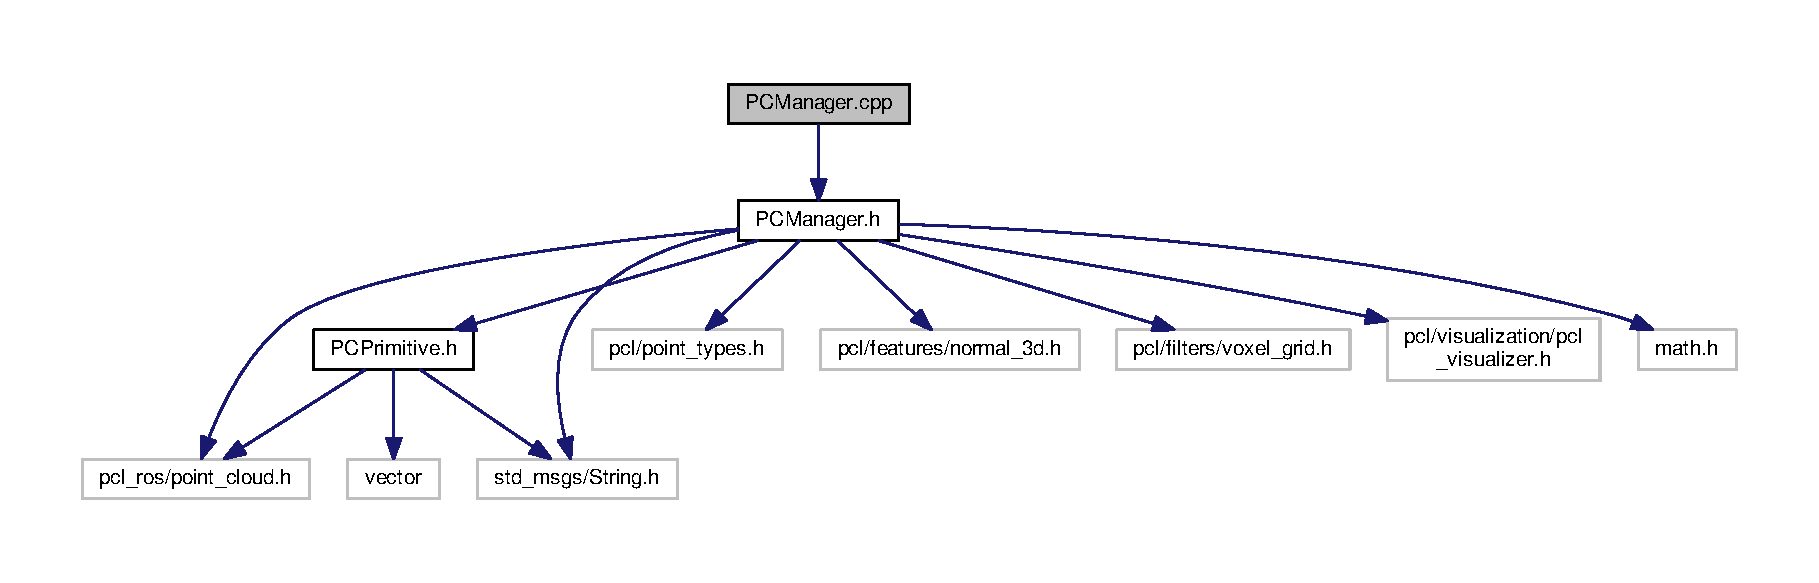
\includegraphics[width=350pt]{PCManager_8cpp__incl}
\end{center}
\end{figure}
\subsection*{Namespaces}
\begin{DoxyCompactItemize}
\item 
\hyperlink{namespacepcm}{pcm}
\end{DoxyCompactItemize}
\subsection*{Functions}
\begin{DoxyCompactItemize}
\item 
static search\-::\-Kd\-Tree\\*
$<$ Point\-X\-Y\-Z $>$\-::Ptr \hyperlink{namespacepcm_a6db83da07339681645ba19a92dbd2046}{pcm\-::tree} (new search\-::\-Kd\-Tree$<$ Point\-X\-Y\-Z $>$())
\end{DoxyCompactItemize}
\subsection*{Variables}
\begin{DoxyCompactItemize}
\item 
static Normal\-Estimation\\*
$<$ Point\-X\-Y\-Z, Normal $>$ \hyperlink{namespacepcm_acbfa006c5c9699694cdf4f598ff57165}{pcm\-::ne}
\item 
static Voxel\-Grid$<$ Point\-X\-Y\-Z $>$ \hyperlink{namespacepcm_a55d9cba2f3ff7122f9162542cde192ac}{pcm\-::sor}
\end{DoxyCompactItemize}

\hypertarget{PCManager_8h}{\section{P\-C\-Manager.\-h File Reference}
\label{PCManager_8h}\index{P\-C\-Manager.\-h@{P\-C\-Manager.\-h}}
}
{\ttfamily \#include $<$pcl\-\_\-ros/point\-\_\-cloud.\-h$>$}\\*
{\ttfamily \#include $<$pcl/point\-\_\-types.\-h$>$}\\*
{\ttfamily \#include $<$pcl/features/normal\-\_\-3d.\-h$>$}\\*
{\ttfamily \#include $<$pcl/filters/voxel\-\_\-grid.\-h$>$}\\*
{\ttfamily \#include $<$pcl/visualization/pcl\-\_\-visualizer.\-h$>$}\\*
{\ttfamily \#include $<$std\-\_\-msgs/\-String.\-h$>$}\\*
{\ttfamily \#include $<$math.\-h$>$}\\*
{\ttfamily \#include \char`\"{}P\-C\-Primitive.\-h\char`\"{}}\\*
Include dependency graph for P\-C\-Manager.\-h\-:\nopagebreak
\begin{figure}[H]
\begin{center}
\leavevmode
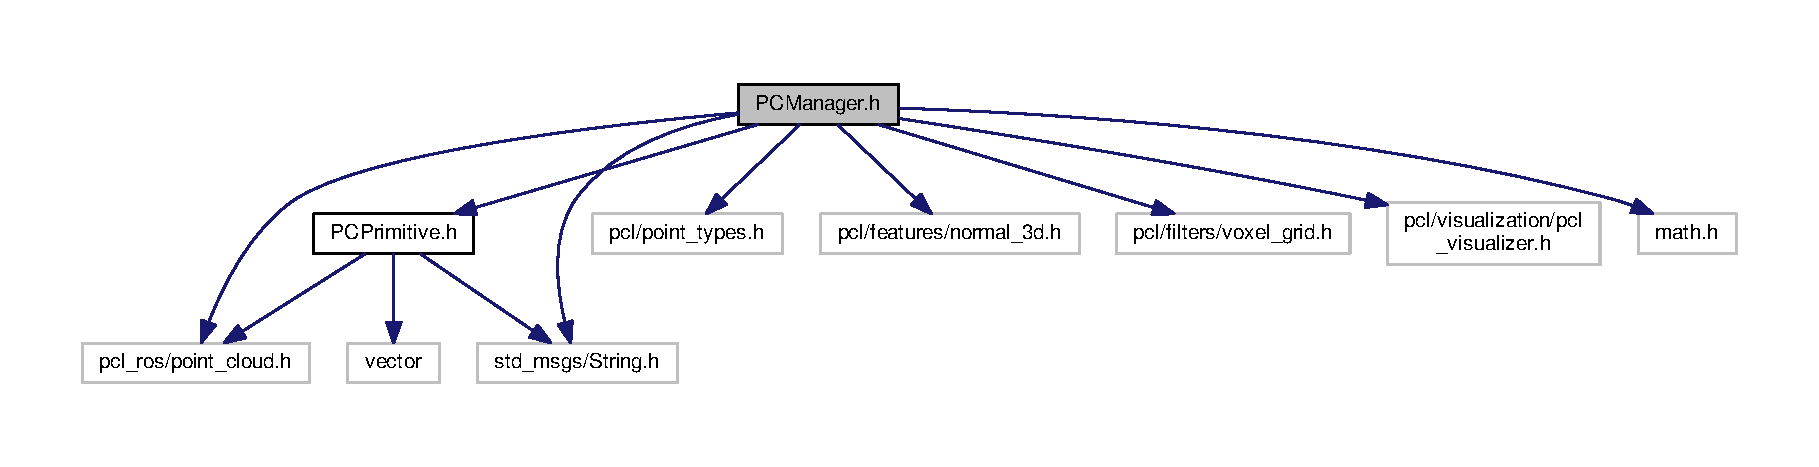
\includegraphics[width=350pt]{PCManager_8h__incl}
\end{center}
\end{figure}
This graph shows which files directly or indirectly include this file\-:\nopagebreak
\begin{figure}[H]
\begin{center}
\leavevmode
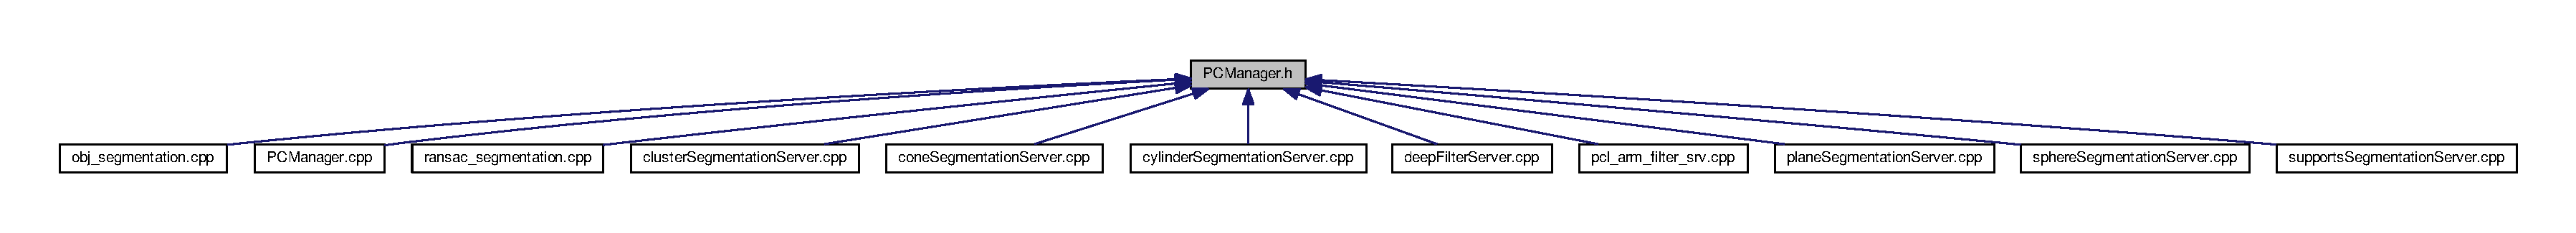
\includegraphics[width=350pt]{PCManager_8h__dep__incl}
\end{center}
\end{figure}
\subsection*{Classes}
\begin{DoxyCompactItemize}
\item 
class \hyperlink{classpcm_1_1PCManager}{pcm\-::\-P\-C\-Manager}
\end{DoxyCompactItemize}
\subsection*{Namespaces}
\begin{DoxyCompactItemize}
\item 
\hyperlink{namespacepcm}{pcm}
\end{DoxyCompactItemize}
\subsection*{Typedefs}
\begin{DoxyCompactItemize}
\item 
typedef boost\-::shared\-\_\-ptr\\*
$<$ \hyperlink{classpcp_1_1PCPrimitive}{pcp\-::\-P\-C\-Primitive} $>$ \hyperlink{PCManager_8h_a0976ac6881bc2fcf1a5503663203e83f}{P\-C\-Primitive\-Ptr}
\item 
typedef boost\-::shared\-\_\-ptr\\*
$<$ visualization\-::\-P\-C\-L\-Visualizer $>$ \hyperlink{PCManager_8h_a38c805dbc7ad6f06109b85c8e540817a}{P\-C\-L\-Visualizer}
\end{DoxyCompactItemize}


\subsection{Typedef Documentation}
\hypertarget{PCManager_8h_a38c805dbc7ad6f06109b85c8e540817a}{\index{P\-C\-Manager.\-h@{P\-C\-Manager.\-h}!P\-C\-L\-Visualizer@{P\-C\-L\-Visualizer}}
\index{P\-C\-L\-Visualizer@{P\-C\-L\-Visualizer}!PCManager.h@{P\-C\-Manager.\-h}}
\subsubsection[{P\-C\-L\-Visualizer}]{\setlength{\rightskip}{0pt plus 5cm}typedef boost\-::shared\-\_\-ptr$<$ visualization\-::\-P\-C\-L\-Visualizer$>$ {\bf P\-C\-L\-Visualizer}}}\label{PCManager_8h_a38c805dbc7ad6f06109b85c8e540817a}


Definition at line 23 of file P\-C\-Manager.\-h.

\hypertarget{PCManager_8h_a0976ac6881bc2fcf1a5503663203e83f}{\index{P\-C\-Manager.\-h@{P\-C\-Manager.\-h}!P\-C\-Primitive\-Ptr@{P\-C\-Primitive\-Ptr}}
\index{P\-C\-Primitive\-Ptr@{P\-C\-Primitive\-Ptr}!PCManager.h@{P\-C\-Manager.\-h}}
\subsubsection[{P\-C\-Primitive\-Ptr}]{\setlength{\rightskip}{0pt plus 5cm}typedef boost\-::shared\-\_\-ptr$<$ {\bf pcp\-::\-P\-C\-Primitive}$>$ {\bf P\-C\-Primitive\-Ptr}}}\label{PCManager_8h_a0976ac6881bc2fcf1a5503663203e83f}


Definition at line 22 of file P\-C\-Manager.\-h.


\hypertarget{PCPrimitive_8cpp}{\section{P\-C\-Primitive.\-cpp File Reference}
\label{PCPrimitive_8cpp}\index{P\-C\-Primitive.\-cpp@{P\-C\-Primitive.\-cpp}}
}
{\ttfamily \#include \char`\"{}P\-C\-Primitive.\-h\char`\"{}}\\*
Include dependency graph for P\-C\-Primitive.\-cpp\-:\nopagebreak
\begin{figure}[H]
\begin{center}
\leavevmode
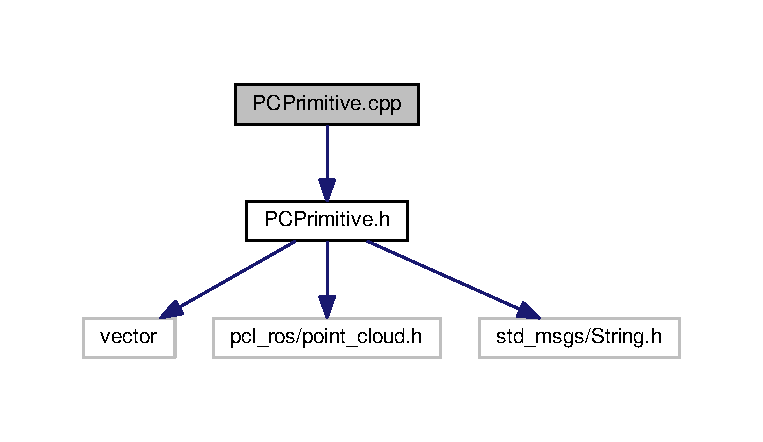
\includegraphics[width=350pt]{PCPrimitive_8cpp__incl}
\end{center}
\end{figure}
\subsection*{Namespaces}
\begin{DoxyCompactItemize}
\item 
\hyperlink{namespacepcp}{pcp}
\end{DoxyCompactItemize}

\hypertarget{PCPrimitive_8h}{\section{P\-C\-Primitive.\-h File Reference}
\label{PCPrimitive_8h}\index{P\-C\-Primitive.\-h@{P\-C\-Primitive.\-h}}
}
{\ttfamily \#include $<$vector$>$}\\*
{\ttfamily \#include $<$pcl\-\_\-ros/point\-\_\-cloud.\-h$>$}\\*
{\ttfamily \#include $<$std\-\_\-msgs/\-String.\-h$>$}\\*
Include dependency graph for P\-C\-Primitive.\-h\-:\nopagebreak
\begin{figure}[H]
\begin{center}
\leavevmode
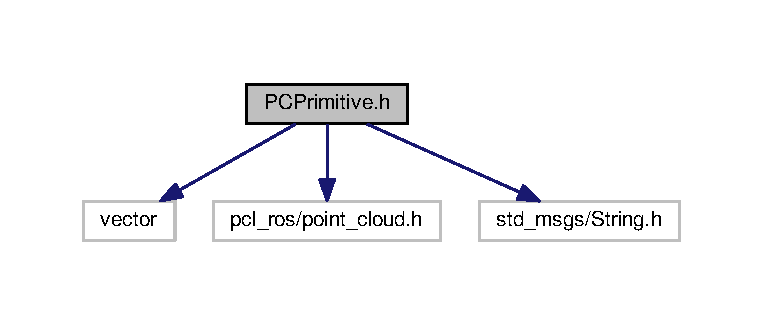
\includegraphics[width=350pt]{PCPrimitive_8h__incl}
\end{center}
\end{figure}
This graph shows which files directly or indirectly include this file\-:\nopagebreak
\begin{figure}[H]
\begin{center}
\leavevmode
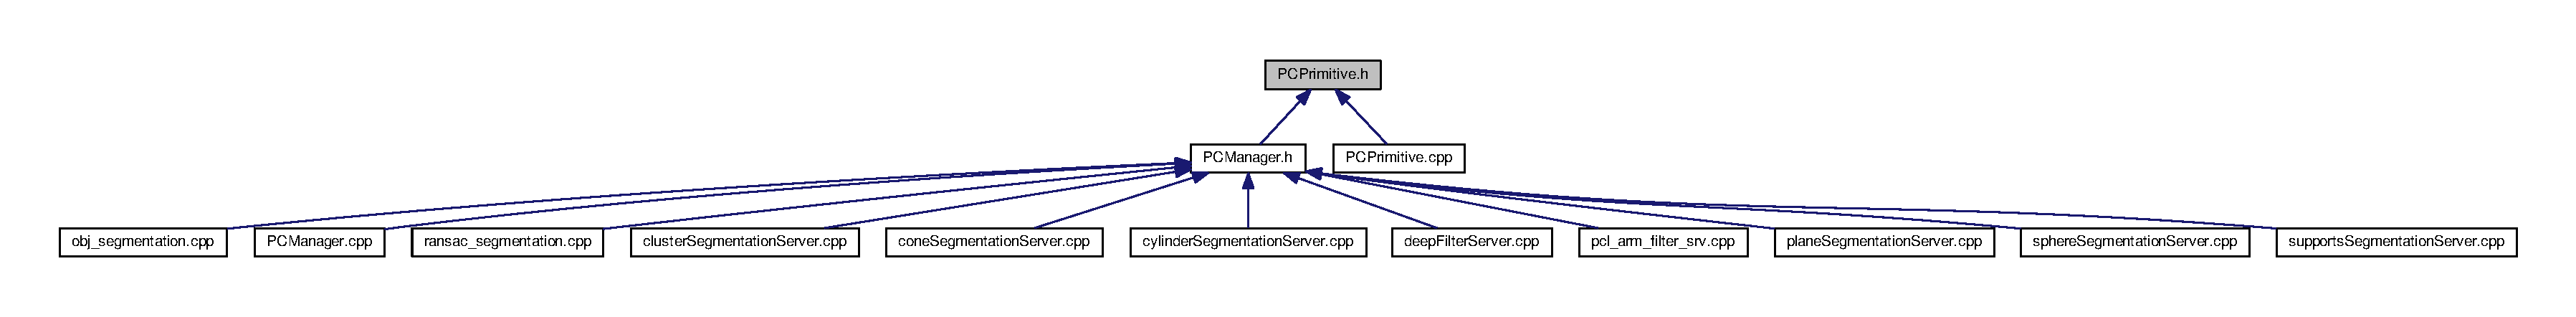
\includegraphics[width=350pt]{PCPrimitive_8h__dep__incl}
\end{center}
\end{figure}
\subsection*{Classes}
\begin{DoxyCompactItemize}
\item 
class \hyperlink{classpcp_1_1PCPrimitive}{pcp\-::\-P\-C\-Primitive}
\end{DoxyCompactItemize}
\subsection*{Namespaces}
\begin{DoxyCompactItemize}
\item 
\hyperlink{namespacepcp}{pcp}
\end{DoxyCompactItemize}
\subsection*{Typedefs}
\begin{DoxyCompactItemize}
\item 
typedef std\-::vector$<$ int $>$ \hyperlink{PCPrimitive_8h_a9aba110b238bb80390c2545da40823e3}{Primitive\-Idx}
\item 
typedef boost\-::shared\-\_\-ptr\\*
$<$ std\-::vector$<$ int $>$ $>$ \hyperlink{PCPrimitive_8h_a6ec0f6fbb026ae4b66cac121673c3a8a}{Primitive\-Idx\-Ptr}
\item 
typedef pcl\-::\-Point\-Cloud\\*
$<$ pcl\-::\-Point\-X\-Y\-Z $>$ \hyperlink{PCPrimitive_8h_a02a7c0cdfcd324f1b5b87ce549fdbe10}{P\-C\-L\-Cloud}
\item 
typedef pcl\-::\-Point\-Cloud\\*
$<$ pcl\-::\-Point\-X\-Y\-Z $>$\-::Ptr \hyperlink{PCPrimitive_8h_aa14a240c8d999c4f56133c0f70e88783}{P\-C\-L\-Cloud\-Ptr}
\item 
typedef pcl\-::\-Point\-Cloud\\*
$<$ pcl\-::\-Normal $>$ \hyperlink{PCPrimitive_8h_abe81b5e6ffcc0ceb1b95b0489419027d}{P\-C\-L\-Normal}
\item 
typedef pcl\-::\-Point\-Cloud\\*
$<$ pcl\-::\-Normal $>$\-::Ptr \hyperlink{PCPrimitive_8h_a1bc38ce8b0c26e5f2d28fae9f3e3ea97}{P\-C\-L\-Normal\-Ptr}
\end{DoxyCompactItemize}


\subsection{Typedef Documentation}
\hypertarget{PCPrimitive_8h_a02a7c0cdfcd324f1b5b87ce549fdbe10}{\index{P\-C\-Primitive.\-h@{P\-C\-Primitive.\-h}!P\-C\-L\-Cloud@{P\-C\-L\-Cloud}}
\index{P\-C\-L\-Cloud@{P\-C\-L\-Cloud}!PCPrimitive.h@{P\-C\-Primitive.\-h}}
\subsubsection[{P\-C\-L\-Cloud}]{\setlength{\rightskip}{0pt plus 5cm}typedef pcl\-::\-Point\-Cloud$<$ pcl\-::\-Point\-X\-Y\-Z$>$ {\bf P\-C\-L\-Cloud}}}\label{PCPrimitive_8h_a02a7c0cdfcd324f1b5b87ce549fdbe10}


Definition at line 20 of file P\-C\-Primitive.\-h.

\hypertarget{PCPrimitive_8h_aa14a240c8d999c4f56133c0f70e88783}{\index{P\-C\-Primitive.\-h@{P\-C\-Primitive.\-h}!P\-C\-L\-Cloud\-Ptr@{P\-C\-L\-Cloud\-Ptr}}
\index{P\-C\-L\-Cloud\-Ptr@{P\-C\-L\-Cloud\-Ptr}!PCPrimitive.h@{P\-C\-Primitive.\-h}}
\subsubsection[{P\-C\-L\-Cloud\-Ptr}]{\setlength{\rightskip}{0pt plus 5cm}typedef pcl\-::\-Point\-Cloud$<$ pcl\-::\-Point\-X\-Y\-Z$>$\-::Ptr {\bf P\-C\-L\-Cloud\-Ptr}}}\label{PCPrimitive_8h_aa14a240c8d999c4f56133c0f70e88783}


Definition at line 21 of file P\-C\-Primitive.\-h.

\hypertarget{PCPrimitive_8h_abe81b5e6ffcc0ceb1b95b0489419027d}{\index{P\-C\-Primitive.\-h@{P\-C\-Primitive.\-h}!P\-C\-L\-Normal@{P\-C\-L\-Normal}}
\index{P\-C\-L\-Normal@{P\-C\-L\-Normal}!PCPrimitive.h@{P\-C\-Primitive.\-h}}
\subsubsection[{P\-C\-L\-Normal}]{\setlength{\rightskip}{0pt plus 5cm}typedef pcl\-::\-Point\-Cloud$<$ pcl\-::\-Normal$>$ {\bf P\-C\-L\-Normal}}}\label{PCPrimitive_8h_abe81b5e6ffcc0ceb1b95b0489419027d}


Definition at line 22 of file P\-C\-Primitive.\-h.

\hypertarget{PCPrimitive_8h_a1bc38ce8b0c26e5f2d28fae9f3e3ea97}{\index{P\-C\-Primitive.\-h@{P\-C\-Primitive.\-h}!P\-C\-L\-Normal\-Ptr@{P\-C\-L\-Normal\-Ptr}}
\index{P\-C\-L\-Normal\-Ptr@{P\-C\-L\-Normal\-Ptr}!PCPrimitive.h@{P\-C\-Primitive.\-h}}
\subsubsection[{P\-C\-L\-Normal\-Ptr}]{\setlength{\rightskip}{0pt plus 5cm}typedef pcl\-::\-Point\-Cloud$<$ pcl\-::\-Normal$>$\-::Ptr {\bf P\-C\-L\-Normal\-Ptr}}}\label{PCPrimitive_8h_a1bc38ce8b0c26e5f2d28fae9f3e3ea97}


Definition at line 23 of file P\-C\-Primitive.\-h.

\hypertarget{PCPrimitive_8h_a9aba110b238bb80390c2545da40823e3}{\index{P\-C\-Primitive.\-h@{P\-C\-Primitive.\-h}!Primitive\-Idx@{Primitive\-Idx}}
\index{Primitive\-Idx@{Primitive\-Idx}!PCPrimitive.h@{P\-C\-Primitive.\-h}}
\subsubsection[{Primitive\-Idx}]{\setlength{\rightskip}{0pt plus 5cm}typedef std\-::vector$<$ int$>$ {\bf Primitive\-Idx}}}\label{PCPrimitive_8h_a9aba110b238bb80390c2545da40823e3}


Definition at line 18 of file P\-C\-Primitive.\-h.

\hypertarget{PCPrimitive_8h_a6ec0f6fbb026ae4b66cac121673c3a8a}{\index{P\-C\-Primitive.\-h@{P\-C\-Primitive.\-h}!Primitive\-Idx\-Ptr@{Primitive\-Idx\-Ptr}}
\index{Primitive\-Idx\-Ptr@{Primitive\-Idx\-Ptr}!PCPrimitive.h@{P\-C\-Primitive.\-h}}
\subsubsection[{Primitive\-Idx\-Ptr}]{\setlength{\rightskip}{0pt plus 5cm}typedef boost\-::shared\-\_\-ptr$<$ std\-::vector$<$ int$>$ $>$ {\bf Primitive\-Idx\-Ptr}}}\label{PCPrimitive_8h_a6ec0f6fbb026ae4b66cac121673c3a8a}


Definition at line 19 of file P\-C\-Primitive.\-h.


\hypertarget{planeSegmentationServer_8cpp}{\section{plane\-Segmentation\-Server.\-cpp File Reference}
\label{planeSegmentationServer_8cpp}\index{plane\-Segmentation\-Server.\-cpp@{plane\-Segmentation\-Server.\-cpp}}
}
{\ttfamily \#include \char`\"{}ros/ros.\-h\char`\"{}}\\*
{\ttfamily \#include $<$pcl\-\_\-ros/point\-\_\-cloud.\-h$>$}\\*
{\ttfamily \#include $<$pcl/segmentation/sac\-\_\-segmentation.\-h$>$}\\*
{\ttfamily \#include \char`\"{}../\-P\-C\-Static\-Processing/\-P\-C\-Manager.\-h\char`\"{}}\\*
{\ttfamily \#include \char`\"{}pitt\-\_\-msgs/\-Primitive\-Segmentation.\-h\char`\"{}}\\*
Include dependency graph for plane\-Segmentation\-Server.\-cpp\-:\nopagebreak
\begin{figure}[H]
\begin{center}
\leavevmode
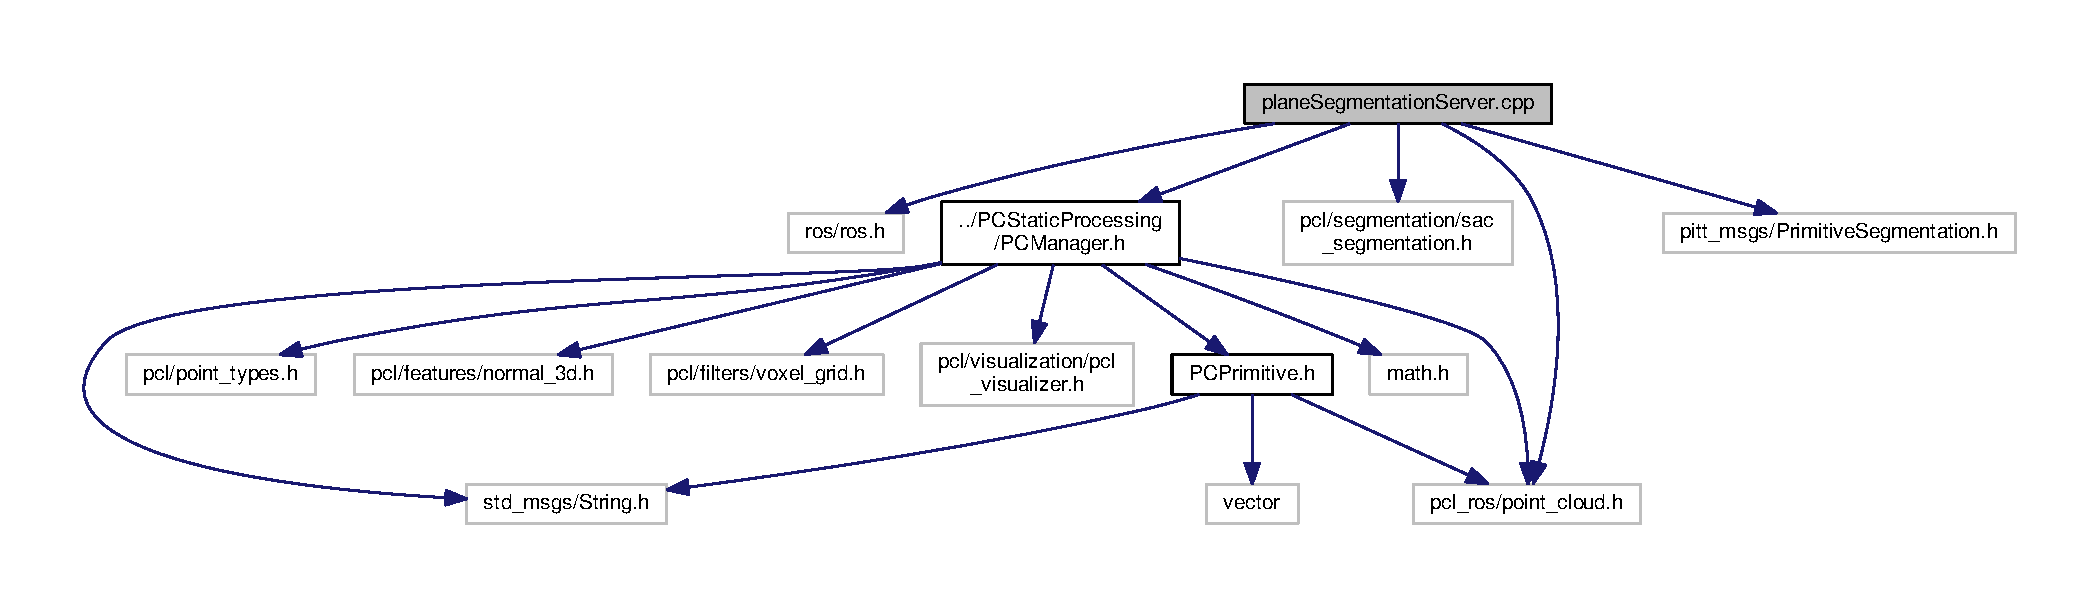
\includegraphics[width=350pt]{planeSegmentationServer_8cpp__incl}
\end{center}
\end{figure}
\subsection*{Functions}
\begin{DoxyCompactItemize}
\item 
bool \hyperlink{planeSegmentationServer_8cpp_a3ed99415e9ed74be38db012266b4e8b1}{ransac\-Plane\-Detaction} (Primitive\-Segmentation\-::\-Request \&req, Primitive\-Segmentation\-::\-Response \&res)
\item 
int \hyperlink{planeSegmentationServer_8cpp_a3c04138a5bfe5d72780bb7e82a18e627}{main} (int argc, char $\ast$$\ast$argv)
\end{DoxyCompactItemize}
\subsection*{Variables}
\begin{DoxyCompactItemize}
\item 
const float \hyperlink{planeSegmentationServer_8cpp_a6a60b5e5200860d75f403dcf05dde9ef}{N\-O\-R\-M\-A\-L\-\_\-\-D\-I\-S\-T\-A\-N\-C\-E\-\_\-\-W\-E\-I\-G\-H\-T\-\_\-\-D\-E\-F\-A\-U\-L\-T} = 0.\-001f
\item 
const float \hyperlink{planeSegmentationServer_8cpp_a73e7be3a150e91558f7c5e69c03dd6e6}{D\-I\-S\-T\-A\-N\-C\-E\-\_\-\-T\-H\-R\-E\-S\-H\-O\-L\-D\-\_\-\-D\-E\-F\-A\-U\-L\-T} = 0.\-007f
\item 
const int \hyperlink{planeSegmentationServer_8cpp_aeb805bfa6116e2c314b0ebc3c73c6504}{M\-A\-X\-\_\-\-I\-T\-E\-R\-A\-T\-I\-O\-N\-\_\-\-D\-E\-F\-A\-U\-L\-T} = 1000
\item 
const float \hyperlink{planeSegmentationServer_8cpp_aa84d6979d2a503e253f54c3e069abaf5}{M\-I\-N\-\_\-\-R\-A\-D\-I\-U\-S\-\_\-\-L\-I\-M\-I\-T} = -\/1.\-0f
\item 
const float \hyperlink{planeSegmentationServer_8cpp_abcdbdc04946f1566041df18c6c892f0f}{M\-A\-X\-\_\-\-R\-A\-D\-I\-U\-S\-\_\-\-L\-I\-M\-I\-T} = -\/1.\-0f
\item 
const float \hyperlink{planeSegmentationServer_8cpp_a32a067fb9ad7cc8e19b52018946d374d}{E\-P\-S\-\_\-\-A\-N\-G\-L\-E} = 0.\-0f
\item 
const float \hyperlink{planeSegmentationServer_8cpp_ae71c4fb043a78285d76d4dcbd7231e70}{M\-I\-N\-\_\-\-O\-P\-E\-N\-I\-N\-G\-\_\-\-A\-N\-G\-L\-E} = 0.\-0f
\item 
const float \hyperlink{planeSegmentationServer_8cpp_afaeeefd6f578a58f8e14040f6176c394}{M\-A\-X\-\_\-\-O\-P\-E\-N\-I\-N\-G\-\_\-\-A\-N\-G\-L\-E} = 10.\-0f
\end{DoxyCompactItemize}


\subsection{Function Documentation}
\hypertarget{planeSegmentationServer_8cpp_a3c04138a5bfe5d72780bb7e82a18e627}{\index{plane\-Segmentation\-Server.\-cpp@{plane\-Segmentation\-Server.\-cpp}!main@{main}}
\index{main@{main}!planeSegmentationServer.cpp@{plane\-Segmentation\-Server.\-cpp}}
\subsubsection[{main}]{\setlength{\rightskip}{0pt plus 5cm}int main (
\begin{DoxyParamCaption}
\item[{int}]{argc, }
\item[{char $\ast$$\ast$}]{argv}
\end{DoxyParamCaption}
)}}\label{planeSegmentationServer_8cpp_a3c04138a5bfe5d72780bb7e82a18e627}


Definition at line 97 of file plane\-Segmentation\-Server.\-cpp.



References pcm\-::\-P\-C\-Manager\-::\-R\-A\-N\-S\-A\-C\-\_\-\-P\-L\-A\-N\-E\-\_\-\-F\-I\-L\-T\-E\-R\-\_\-\-S\-E\-R\-V\-I\-C\-E\-\_\-\-N\-A\-M\-E, and ransac\-Plane\-Detaction().



Here is the call graph for this function\-:\nopagebreak
\begin{figure}[H]
\begin{center}
\leavevmode
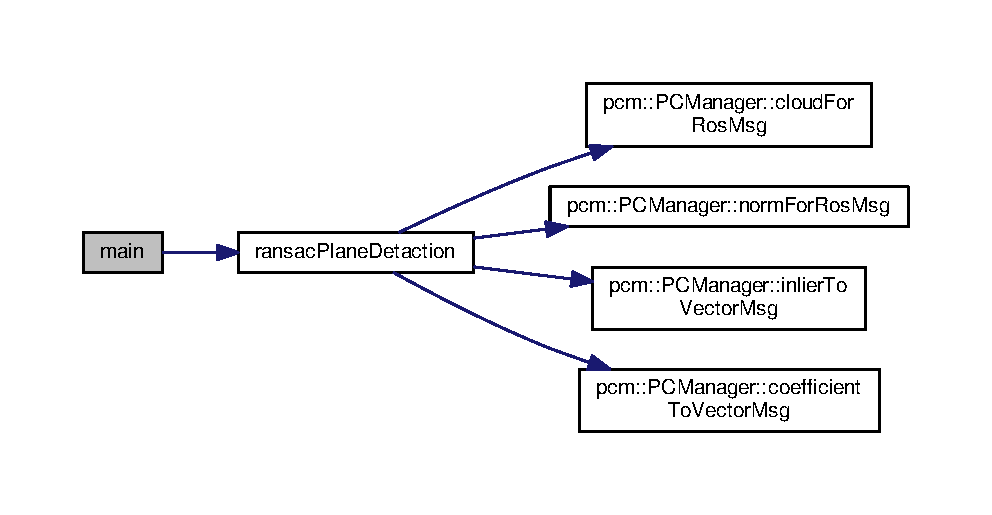
\includegraphics[width=350pt]{planeSegmentationServer_8cpp_a3c04138a5bfe5d72780bb7e82a18e627_cgraph}
\end{center}
\end{figure}


\hypertarget{planeSegmentationServer_8cpp_a3ed99415e9ed74be38db012266b4e8b1}{\index{plane\-Segmentation\-Server.\-cpp@{plane\-Segmentation\-Server.\-cpp}!ransac\-Plane\-Detaction@{ransac\-Plane\-Detaction}}
\index{ransac\-Plane\-Detaction@{ransac\-Plane\-Detaction}!planeSegmentationServer.cpp@{plane\-Segmentation\-Server.\-cpp}}
\subsubsection[{ransac\-Plane\-Detaction}]{\setlength{\rightskip}{0pt plus 5cm}bool ransac\-Plane\-Detaction (
\begin{DoxyParamCaption}
\item[{Primitive\-Segmentation\-::\-Request \&}]{req, }
\item[{Primitive\-Segmentation\-::\-Response \&}]{res}
\end{DoxyParamCaption}
)}}\label{planeSegmentationServer_8cpp_a3ed99415e9ed74be38db012266b4e8b1}


Definition at line 25 of file plane\-Segmentation\-Server.\-cpp.



References pcm\-::\-P\-C\-Manager\-::cloud\-For\-Ros\-Msg(), pcm\-::\-P\-C\-Manager\-::coefficient\-To\-Vector\-Msg(), D\-I\-S\-T\-A\-N\-C\-E\-\_\-\-T\-H\-R\-E\-S\-H\-O\-L\-D\-\_\-\-D\-E\-F\-A\-U\-L\-T, E\-P\-S\-\_\-\-A\-N\-G\-L\-E, pcm\-::\-P\-C\-Manager\-::inlier\-To\-Vector\-Msg(), M\-A\-X\-\_\-\-I\-T\-E\-R\-A\-T\-I\-O\-N\-\_\-\-D\-E\-F\-A\-U\-L\-T, M\-A\-X\-\_\-\-O\-P\-E\-N\-I\-N\-G\-\_\-\-A\-N\-G\-L\-E, M\-A\-X\-\_\-\-R\-A\-D\-I\-U\-S\-\_\-\-L\-I\-M\-I\-T, M\-I\-N\-\_\-\-O\-P\-E\-N\-I\-N\-G\-\_\-\-A\-N\-G\-L\-E, M\-I\-N\-\_\-\-R\-A\-D\-I\-U\-S\-\_\-\-L\-I\-M\-I\-T, N\-O\-R\-M\-A\-L\-\_\-\-D\-I\-S\-T\-A\-N\-C\-E\-\_\-\-W\-E\-I\-G\-H\-T\-\_\-\-D\-E\-F\-A\-U\-L\-T, pcm\-::\-P\-C\-Manager\-::norm\-For\-Ros\-Msg(), and seg.



Referenced by main().



Here is the call graph for this function\-:\nopagebreak
\begin{figure}[H]
\begin{center}
\leavevmode
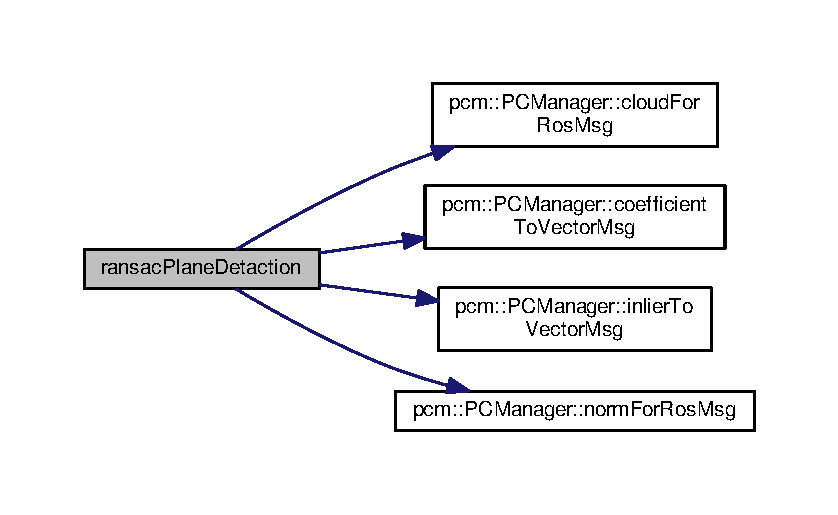
\includegraphics[width=350pt]{planeSegmentationServer_8cpp_a3ed99415e9ed74be38db012266b4e8b1_cgraph}
\end{center}
\end{figure}




\subsection{Variable Documentation}
\hypertarget{planeSegmentationServer_8cpp_a73e7be3a150e91558f7c5e69c03dd6e6}{\index{plane\-Segmentation\-Server.\-cpp@{plane\-Segmentation\-Server.\-cpp}!D\-I\-S\-T\-A\-N\-C\-E\-\_\-\-T\-H\-R\-E\-S\-H\-O\-L\-D\-\_\-\-D\-E\-F\-A\-U\-L\-T@{D\-I\-S\-T\-A\-N\-C\-E\-\_\-\-T\-H\-R\-E\-S\-H\-O\-L\-D\-\_\-\-D\-E\-F\-A\-U\-L\-T}}
\index{D\-I\-S\-T\-A\-N\-C\-E\-\_\-\-T\-H\-R\-E\-S\-H\-O\-L\-D\-\_\-\-D\-E\-F\-A\-U\-L\-T@{D\-I\-S\-T\-A\-N\-C\-E\-\_\-\-T\-H\-R\-E\-S\-H\-O\-L\-D\-\_\-\-D\-E\-F\-A\-U\-L\-T}!planeSegmentationServer.cpp@{plane\-Segmentation\-Server.\-cpp}}
\subsubsection[{D\-I\-S\-T\-A\-N\-C\-E\-\_\-\-T\-H\-R\-E\-S\-H\-O\-L\-D\-\_\-\-D\-E\-F\-A\-U\-L\-T}]{\setlength{\rightskip}{0pt plus 5cm}const float D\-I\-S\-T\-A\-N\-C\-E\-\_\-\-T\-H\-R\-E\-S\-H\-O\-L\-D\-\_\-\-D\-E\-F\-A\-U\-L\-T = 0.\-007f}}\label{planeSegmentationServer_8cpp_a73e7be3a150e91558f7c5e69c03dd6e6}


Definition at line 16 of file plane\-Segmentation\-Server.\-cpp.



Referenced by ransac\-Plane\-Detaction().

\hypertarget{planeSegmentationServer_8cpp_a32a067fb9ad7cc8e19b52018946d374d}{\index{plane\-Segmentation\-Server.\-cpp@{plane\-Segmentation\-Server.\-cpp}!E\-P\-S\-\_\-\-A\-N\-G\-L\-E@{E\-P\-S\-\_\-\-A\-N\-G\-L\-E}}
\index{E\-P\-S\-\_\-\-A\-N\-G\-L\-E@{E\-P\-S\-\_\-\-A\-N\-G\-L\-E}!planeSegmentationServer.cpp@{plane\-Segmentation\-Server.\-cpp}}
\subsubsection[{E\-P\-S\-\_\-\-A\-N\-G\-L\-E}]{\setlength{\rightskip}{0pt plus 5cm}const float E\-P\-S\-\_\-\-A\-N\-G\-L\-E = 0.\-0f}}\label{planeSegmentationServer_8cpp_a32a067fb9ad7cc8e19b52018946d374d}


Definition at line 20 of file plane\-Segmentation\-Server.\-cpp.



Referenced by ransac\-Plane\-Detaction().

\hypertarget{planeSegmentationServer_8cpp_aeb805bfa6116e2c314b0ebc3c73c6504}{\index{plane\-Segmentation\-Server.\-cpp@{plane\-Segmentation\-Server.\-cpp}!M\-A\-X\-\_\-\-I\-T\-E\-R\-A\-T\-I\-O\-N\-\_\-\-D\-E\-F\-A\-U\-L\-T@{M\-A\-X\-\_\-\-I\-T\-E\-R\-A\-T\-I\-O\-N\-\_\-\-D\-E\-F\-A\-U\-L\-T}}
\index{M\-A\-X\-\_\-\-I\-T\-E\-R\-A\-T\-I\-O\-N\-\_\-\-D\-E\-F\-A\-U\-L\-T@{M\-A\-X\-\_\-\-I\-T\-E\-R\-A\-T\-I\-O\-N\-\_\-\-D\-E\-F\-A\-U\-L\-T}!planeSegmentationServer.cpp@{plane\-Segmentation\-Server.\-cpp}}
\subsubsection[{M\-A\-X\-\_\-\-I\-T\-E\-R\-A\-T\-I\-O\-N\-\_\-\-D\-E\-F\-A\-U\-L\-T}]{\setlength{\rightskip}{0pt plus 5cm}const int M\-A\-X\-\_\-\-I\-T\-E\-R\-A\-T\-I\-O\-N\-\_\-\-D\-E\-F\-A\-U\-L\-T = 1000}}\label{planeSegmentationServer_8cpp_aeb805bfa6116e2c314b0ebc3c73c6504}


Definition at line 17 of file plane\-Segmentation\-Server.\-cpp.



Referenced by ransac\-Plane\-Detaction().

\hypertarget{planeSegmentationServer_8cpp_afaeeefd6f578a58f8e14040f6176c394}{\index{plane\-Segmentation\-Server.\-cpp@{plane\-Segmentation\-Server.\-cpp}!M\-A\-X\-\_\-\-O\-P\-E\-N\-I\-N\-G\-\_\-\-A\-N\-G\-L\-E@{M\-A\-X\-\_\-\-O\-P\-E\-N\-I\-N\-G\-\_\-\-A\-N\-G\-L\-E}}
\index{M\-A\-X\-\_\-\-O\-P\-E\-N\-I\-N\-G\-\_\-\-A\-N\-G\-L\-E@{M\-A\-X\-\_\-\-O\-P\-E\-N\-I\-N\-G\-\_\-\-A\-N\-G\-L\-E}!planeSegmentationServer.cpp@{plane\-Segmentation\-Server.\-cpp}}
\subsubsection[{M\-A\-X\-\_\-\-O\-P\-E\-N\-I\-N\-G\-\_\-\-A\-N\-G\-L\-E}]{\setlength{\rightskip}{0pt plus 5cm}const float M\-A\-X\-\_\-\-O\-P\-E\-N\-I\-N\-G\-\_\-\-A\-N\-G\-L\-E = 10.\-0f}}\label{planeSegmentationServer_8cpp_afaeeefd6f578a58f8e14040f6176c394}


Definition at line 22 of file plane\-Segmentation\-Server.\-cpp.



Referenced by ransac\-Plane\-Detaction().

\hypertarget{planeSegmentationServer_8cpp_abcdbdc04946f1566041df18c6c892f0f}{\index{plane\-Segmentation\-Server.\-cpp@{plane\-Segmentation\-Server.\-cpp}!M\-A\-X\-\_\-\-R\-A\-D\-I\-U\-S\-\_\-\-L\-I\-M\-I\-T@{M\-A\-X\-\_\-\-R\-A\-D\-I\-U\-S\-\_\-\-L\-I\-M\-I\-T}}
\index{M\-A\-X\-\_\-\-R\-A\-D\-I\-U\-S\-\_\-\-L\-I\-M\-I\-T@{M\-A\-X\-\_\-\-R\-A\-D\-I\-U\-S\-\_\-\-L\-I\-M\-I\-T}!planeSegmentationServer.cpp@{plane\-Segmentation\-Server.\-cpp}}
\subsubsection[{M\-A\-X\-\_\-\-R\-A\-D\-I\-U\-S\-\_\-\-L\-I\-M\-I\-T}]{\setlength{\rightskip}{0pt plus 5cm}const float M\-A\-X\-\_\-\-R\-A\-D\-I\-U\-S\-\_\-\-L\-I\-M\-I\-T = -\/1.\-0f}}\label{planeSegmentationServer_8cpp_abcdbdc04946f1566041df18c6c892f0f}


Definition at line 19 of file plane\-Segmentation\-Server.\-cpp.



Referenced by ransac\-Plane\-Detaction().

\hypertarget{planeSegmentationServer_8cpp_ae71c4fb043a78285d76d4dcbd7231e70}{\index{plane\-Segmentation\-Server.\-cpp@{plane\-Segmentation\-Server.\-cpp}!M\-I\-N\-\_\-\-O\-P\-E\-N\-I\-N\-G\-\_\-\-A\-N\-G\-L\-E@{M\-I\-N\-\_\-\-O\-P\-E\-N\-I\-N\-G\-\_\-\-A\-N\-G\-L\-E}}
\index{M\-I\-N\-\_\-\-O\-P\-E\-N\-I\-N\-G\-\_\-\-A\-N\-G\-L\-E@{M\-I\-N\-\_\-\-O\-P\-E\-N\-I\-N\-G\-\_\-\-A\-N\-G\-L\-E}!planeSegmentationServer.cpp@{plane\-Segmentation\-Server.\-cpp}}
\subsubsection[{M\-I\-N\-\_\-\-O\-P\-E\-N\-I\-N\-G\-\_\-\-A\-N\-G\-L\-E}]{\setlength{\rightskip}{0pt plus 5cm}const float M\-I\-N\-\_\-\-O\-P\-E\-N\-I\-N\-G\-\_\-\-A\-N\-G\-L\-E = 0.\-0f}}\label{planeSegmentationServer_8cpp_ae71c4fb043a78285d76d4dcbd7231e70}


Definition at line 21 of file plane\-Segmentation\-Server.\-cpp.



Referenced by ransac\-Plane\-Detaction().

\hypertarget{planeSegmentationServer_8cpp_aa84d6979d2a503e253f54c3e069abaf5}{\index{plane\-Segmentation\-Server.\-cpp@{plane\-Segmentation\-Server.\-cpp}!M\-I\-N\-\_\-\-R\-A\-D\-I\-U\-S\-\_\-\-L\-I\-M\-I\-T@{M\-I\-N\-\_\-\-R\-A\-D\-I\-U\-S\-\_\-\-L\-I\-M\-I\-T}}
\index{M\-I\-N\-\_\-\-R\-A\-D\-I\-U\-S\-\_\-\-L\-I\-M\-I\-T@{M\-I\-N\-\_\-\-R\-A\-D\-I\-U\-S\-\_\-\-L\-I\-M\-I\-T}!planeSegmentationServer.cpp@{plane\-Segmentation\-Server.\-cpp}}
\subsubsection[{M\-I\-N\-\_\-\-R\-A\-D\-I\-U\-S\-\_\-\-L\-I\-M\-I\-T}]{\setlength{\rightskip}{0pt plus 5cm}const float M\-I\-N\-\_\-\-R\-A\-D\-I\-U\-S\-\_\-\-L\-I\-M\-I\-T = -\/1.\-0f}}\label{planeSegmentationServer_8cpp_aa84d6979d2a503e253f54c3e069abaf5}


Definition at line 18 of file plane\-Segmentation\-Server.\-cpp.



Referenced by ransac\-Plane\-Detaction().

\hypertarget{planeSegmentationServer_8cpp_a6a60b5e5200860d75f403dcf05dde9ef}{\index{plane\-Segmentation\-Server.\-cpp@{plane\-Segmentation\-Server.\-cpp}!N\-O\-R\-M\-A\-L\-\_\-\-D\-I\-S\-T\-A\-N\-C\-E\-\_\-\-W\-E\-I\-G\-H\-T\-\_\-\-D\-E\-F\-A\-U\-L\-T@{N\-O\-R\-M\-A\-L\-\_\-\-D\-I\-S\-T\-A\-N\-C\-E\-\_\-\-W\-E\-I\-G\-H\-T\-\_\-\-D\-E\-F\-A\-U\-L\-T}}
\index{N\-O\-R\-M\-A\-L\-\_\-\-D\-I\-S\-T\-A\-N\-C\-E\-\_\-\-W\-E\-I\-G\-H\-T\-\_\-\-D\-E\-F\-A\-U\-L\-T@{N\-O\-R\-M\-A\-L\-\_\-\-D\-I\-S\-T\-A\-N\-C\-E\-\_\-\-W\-E\-I\-G\-H\-T\-\_\-\-D\-E\-F\-A\-U\-L\-T}!planeSegmentationServer.cpp@{plane\-Segmentation\-Server.\-cpp}}
\subsubsection[{N\-O\-R\-M\-A\-L\-\_\-\-D\-I\-S\-T\-A\-N\-C\-E\-\_\-\-W\-E\-I\-G\-H\-T\-\_\-\-D\-E\-F\-A\-U\-L\-T}]{\setlength{\rightskip}{0pt plus 5cm}const float N\-O\-R\-M\-A\-L\-\_\-\-D\-I\-S\-T\-A\-N\-C\-E\-\_\-\-W\-E\-I\-G\-H\-T\-\_\-\-D\-E\-F\-A\-U\-L\-T = 0.\-001f}}\label{planeSegmentationServer_8cpp_a6a60b5e5200860d75f403dcf05dde9ef}


Definition at line 15 of file plane\-Segmentation\-Server.\-cpp.



Referenced by ransac\-Plane\-Detaction().


\hypertarget{ransac__segmentation_8cpp}{\section{ransac\-\_\-segmentation.\-cpp File Reference}
\label{ransac__segmentation_8cpp}\index{ransac\-\_\-segmentation.\-cpp@{ransac\-\_\-segmentation.\-cpp}}
}
{\ttfamily \#include \char`\"{}P\-C\-Static\-Processing/\-P\-C\-Manager.\-h\char`\"{}}\\*
{\ttfamily \#include \char`\"{}pitt\-\_\-msgs/\-Clusters\-Output.\-h\char`\"{}}\\*
{\ttfamily \#include \char`\"{}pitt\-\_\-msgs/\-Inliers\-Cluster.\-h\char`\"{}}\\*
{\ttfamily \#include \char`\"{}pitt\-\_\-msgs/\-Primitive\-Segmentation.\-h\char`\"{}}\\*
{\ttfamily \#include \char`\"{}pitt\-\_\-msgs/\-Tracked\-Shapes.\-h\char`\"{}}\\*
{\ttfamily \#include \char`\"{}pitt\-\_\-msgs/\-Tracked\-Shape.\-h\char`\"{}}\\*
{\ttfamily \#include \char`\"{}pitt\-\_\-msgs/\-Semantic\-Scene\-Recogniton.\-h\char`\"{}}\\*
Include dependency graph for ransac\-\_\-segmentation.\-cpp\-:\nopagebreak
\begin{figure}[H]
\begin{center}
\leavevmode
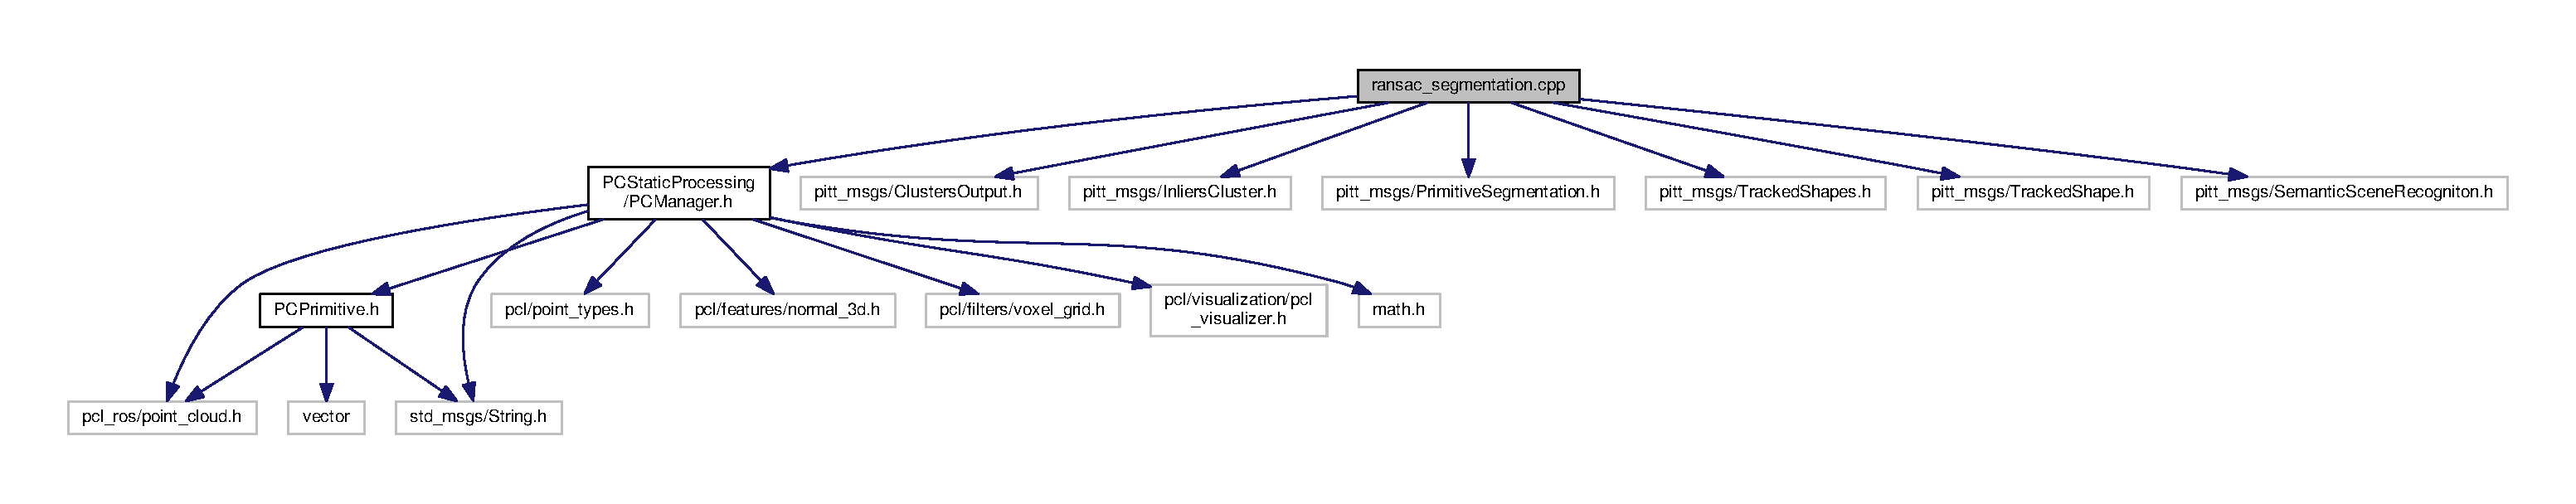
\includegraphics[width=350pt]{ransac__segmentation_8cpp__incl}
\end{center}
\end{figure}
\subsection*{Typedefs}
\begin{DoxyCompactItemize}
\item 
typedef vector$<$ Inliers\-Cluster $>$ \hyperlink{ransac__segmentation_8cpp_a48bae868bfe27bed6e11eeb5c77b062a}{Inliers\-Clusters}
\item 
typedef boost\-::shared\-\_\-ptr\\*
$<$ \hyperlink{ransac__segmentation_8cpp_a48bae868bfe27bed6e11eeb5c77b062a}{Inliers\-Clusters} $>$ \hyperlink{ransac__segmentation_8cpp_af1cdfa162edb0b94902557379b5cf42d}{Inliers\-Clusters\-Ptr}
\item 
typedef boost\-::shared\-\_\-ptr\\*
$<$ Primitive\-Segmentation $>$ \hyperlink{ransac__segmentation_8cpp_aadce7a04d47ab4d0099588791d834045}{Primitive\-Segmentation\-Ptr}
\end{DoxyCompactItemize}
\subsection*{Functions}
\begin{DoxyCompactItemize}
\item 
bool \hyperlink{ransac__segmentation_8cpp_a1c975f4a118598c3ab7eff48fa749476}{call\-Ransac\-Sphere\-Segmentation} (\hyperlink{PCPrimitive_8h_aa14a240c8d999c4f56133c0f70e88783}{P\-C\-L\-Cloud\-Ptr} cloud, \hyperlink{PCPrimitive_8h_a1bc38ce8b0c26e5f2d28fae9f3e3ea97}{P\-C\-L\-Normal\-Ptr} norm, \hyperlink{ransac__segmentation_8cpp_aadce7a04d47ab4d0099588791d834045}{Primitive\-Segmentation\-Ptr} \&out)
\item 
void \hyperlink{ransac__segmentation_8cpp_a575e2f0efaeee850e608ac4481557314}{print\-Sphere\-Info} (\hyperlink{ransac__segmentation_8cpp_aadce7a04d47ab4d0099588791d834045}{Primitive\-Segmentation\-Ptr} info, int idx)
\item 
bool \hyperlink{ransac__segmentation_8cpp_a850aede9ccf4da9338681e9ea25b50c6}{call\-Ransac\-Cylinder\-Segmentation} (\hyperlink{PCPrimitive_8h_aa14a240c8d999c4f56133c0f70e88783}{P\-C\-L\-Cloud\-Ptr} cloud, \hyperlink{PCPrimitive_8h_a1bc38ce8b0c26e5f2d28fae9f3e3ea97}{P\-C\-L\-Normal\-Ptr} norm, \hyperlink{ransac__segmentation_8cpp_aadce7a04d47ab4d0099588791d834045}{Primitive\-Segmentation\-Ptr} \&out)
\item 
void \hyperlink{ransac__segmentation_8cpp_a45c30fa927c0717d8346839fd1c68bde}{print\-Cylinder\-Info} (\hyperlink{ransac__segmentation_8cpp_aadce7a04d47ab4d0099588791d834045}{Primitive\-Segmentation\-Ptr} info, int idx)
\item 
bool \hyperlink{ransac__segmentation_8cpp_aec52b04d4f14e655979ec0316bab27be}{call\-Ransac\-Cone\-Segmentation} (\hyperlink{PCPrimitive_8h_aa14a240c8d999c4f56133c0f70e88783}{P\-C\-L\-Cloud\-Ptr} cloud, \hyperlink{PCPrimitive_8h_a1bc38ce8b0c26e5f2d28fae9f3e3ea97}{P\-C\-L\-Normal\-Ptr} norm, \hyperlink{ransac__segmentation_8cpp_aadce7a04d47ab4d0099588791d834045}{Primitive\-Segmentation\-Ptr} \&out)
\item 
void \hyperlink{ransac__segmentation_8cpp_a7e84119f095d7369dc280ca585dcd9fb}{print\-Cone\-Info} (\hyperlink{ransac__segmentation_8cpp_aadce7a04d47ab4d0099588791d834045}{Primitive\-Segmentation\-Ptr} info, int idx)
\item 
bool \hyperlink{ransac__segmentation_8cpp_afcfa79d6f194e0e582affcad49fec033}{call\-Ransac\-Plane\-Segmentation} (\hyperlink{PCPrimitive_8h_aa14a240c8d999c4f56133c0f70e88783}{P\-C\-L\-Cloud\-Ptr} cloud, \hyperlink{PCPrimitive_8h_a1bc38ce8b0c26e5f2d28fae9f3e3ea97}{P\-C\-L\-Normal\-Ptr} norm, \hyperlink{ransac__segmentation_8cpp_aadce7a04d47ab4d0099588791d834045}{Primitive\-Segmentation\-Ptr} \&out)
\item 
void \hyperlink{ransac__segmentation_8cpp_a20792e9769230baa8e2258731a5143de}{print\-Plane\-Info} (\hyperlink{ransac__segmentation_8cpp_aadce7a04d47ab4d0099588791d834045}{Primitive\-Segmentation\-Ptr} info, int idx)
\item 
string \hyperlink{ransac__segmentation_8cpp_a9fce32945b78e03d2b0abde7198fe623}{return\-Primitive\-Name\-From\-Tag} (int primitive\-Tag)
\item 
bool \hyperlink{ransac__segmentation_8cpp_a8f13fc832e8677f944e83fb870b8b6a0}{call\-Semantic\-Scene\-Recognition\-Server} (Tracked\-Shapes\-::\-Ptr out\-Shapes)
\item 
void \hyperlink{ransac__segmentation_8cpp_a87bb87e16486622aae18704555f5af81}{clusters\-Acquisition} (const Clusters\-Output\-Const\-Ptr \&cluster\-Obj)
\item 
int \hyperlink{ransac__segmentation_8cpp_a3c04138a5bfe5d72780bb7e82a18e627}{main} (int argc, char $\ast$$\ast$argv)
\end{DoxyCompactItemize}
\subsection*{Variables}
\begin{DoxyCompactItemize}
\item 
boost\-::shared\-\_\-ptr\\*
$<$ \hyperlink{PCManager_8h_a38c805dbc7ad6f06109b85c8e540817a}{visualization\-::\-P\-C\-L\-Visualizer} $>$ \hyperlink{ransac__segmentation_8cpp_a6c2d87234fca8dcca11f888098558986}{vis}
\item 
Publisher \hyperlink{ransac__segmentation_8cpp_a13f806db112b4cc50fbdc2bc57078c28}{pub}
\item 
static const float \hyperlink{ransac__segmentation_8cpp_ab59ca1c04d41c87beeae6d1c978c163c}{S\-P\-H\-E\-R\-E\-\_\-\-N\-O\-R\-M\-A\-L\-\_\-\-D\-I\-S\-T\-A\-N\-C\-E\-\_\-\-W\-E\-I\-G\-T\-H} = P\-C\-Manager\-::\-D\-E\-F\-A\-U\-L\-T\-\_\-\-S\-E\-R\-V\-I\-C\-E\-\_\-\-P\-A\-R\-A\-M\-E\-T\-E\-R\-\_\-\-R\-E\-Q\-U\-E\-S\-T
\item 
static const float \hyperlink{ransac__segmentation_8cpp_ae660f7defcf0829dc6021c4f0f004679}{S\-P\-H\-E\-R\-E\-\_\-\-D\-I\-S\-T\-A\-N\-Z\-E\-\_\-\-T\-H} = P\-C\-Manager\-::\-D\-E\-F\-A\-U\-L\-T\-\_\-\-S\-E\-R\-V\-I\-C\-E\-\_\-\-P\-A\-R\-A\-M\-E\-T\-E\-R\-\_\-\-R\-E\-Q\-U\-E\-S\-T
\item 
static const float \hyperlink{ransac__segmentation_8cpp_abf8dbd1b3ebbdae66c8d1ff0879d343e}{S\-P\-H\-E\-R\-E\-\_\-\-M\-I\-N\-\_\-\-R\-A\-D\-I\-U\-S\-\_\-\-L\-I\-M\-I\-T} = P\-C\-Manager\-::\-D\-E\-F\-A\-U\-L\-T\-\_\-\-S\-E\-R\-V\-I\-C\-E\-\_\-\-P\-A\-R\-A\-M\-E\-T\-E\-R\-\_\-\-R\-E\-Q\-U\-E\-S\-T
\item 
static const float \hyperlink{ransac__segmentation_8cpp_a7f4eca0782eab553a5b0df2dfe042627}{S\-P\-H\-E\-R\-E\-\_\-\-M\-A\-X\-\_\-\-R\-A\-D\-I\-U\-S\-\_\-\-L\-I\-M\-I\-T} = P\-C\-Manager\-::\-D\-E\-F\-A\-U\-L\-T\-\_\-\-S\-E\-R\-V\-I\-C\-E\-\_\-\-P\-A\-R\-A\-M\-E\-T\-E\-R\-\_\-\-R\-E\-Q\-U\-E\-S\-T
\item 
static const int \hyperlink{ransac__segmentation_8cpp_a957f1a2151039b32d471c06adb64991a}{S\-P\-H\-E\-R\-E\-\_\-\-M\-A\-X\-\_\-\-I\-T\-E\-R\-A\-T\-I\-O\-N\-\_\-\-L\-I\-M\-I\-T} = P\-C\-Manager\-::\-D\-E\-F\-A\-U\-L\-T\-\_\-\-S\-E\-R\-V\-I\-C\-E\-\_\-\-P\-A\-R\-A\-M\-E\-T\-E\-R\-\_\-\-R\-E\-Q\-U\-E\-S\-T
\item 
static const float \hyperlink{ransac__segmentation_8cpp_a4457ce4b0cafdb5bb1a2463d32c04750}{S\-P\-H\-E\-R\-E\-\_\-\-E\-P\-S\-\_\-\-A\-N\-G\-L\-E\-\_\-\-T\-H} = P\-C\-Manager\-::\-D\-E\-F\-A\-U\-L\-T\-\_\-\-S\-E\-R\-V\-I\-C\-E\-\_\-\-P\-A\-R\-A\-M\-E\-T\-E\-R\-\_\-\-R\-E\-Q\-U\-E\-S\-T
\item 
static const float \hyperlink{ransac__segmentation_8cpp_a3fcbd31ec09d5e4a35a850c696a9e40d}{S\-P\-H\-E\-R\-E\-\_\-\-M\-I\-N\-\_\-\-O\-P\-E\-N\-I\-N\-G\-\_\-\-A\-N\-G\-L\-E\-\_\-\-D\-E\-G\-R\-E\-E} = P\-C\-Manager\-::\-D\-E\-F\-A\-U\-L\-T\-\_\-\-S\-E\-R\-V\-I\-C\-E\-\_\-\-P\-A\-R\-A\-M\-E\-T\-E\-R\-\_\-\-R\-E\-Q\-U\-E\-S\-T
\item 
static const float \hyperlink{ransac__segmentation_8cpp_a70500987db7dd28ae7e9c862f56c8e5d}{S\-P\-H\-E\-R\-E\-\_\-\-M\-A\-X\-\_\-\-O\-P\-E\-N\-I\-N\-G\-\_\-\-A\-N\-G\-L\-E\-\_\-\-D\-E\-G\-R\-E\-E} = P\-C\-Manager\-::\-D\-E\-F\-A\-U\-L\-T\-\_\-\-S\-E\-R\-V\-I\-C\-E\-\_\-\-P\-A\-R\-A\-M\-E\-T\-E\-R\-\_\-\-R\-E\-Q\-U\-E\-S\-T
\item 
static const int \hyperlink{ransac__segmentation_8cpp_a2972fa461f1c436f915bd64eeb7c431f}{S\-P\-H\-E\-R\-E\-\_\-\-M\-I\-N\-\_\-\-I\-N\-L\-I\-E\-R\-S} = 40
\item 
static const float \hyperlink{ransac__segmentation_8cpp_a343ca34ce396f1e85c6e4c76889006ad}{C\-Y\-L\-I\-N\-D\-E\-R\-\_\-\-N\-O\-R\-M\-A\-L\-\_\-\-D\-I\-S\-T\-A\-N\-C\-E\-\_\-\-W\-E\-I\-G\-T\-H} = P\-C\-Manager\-::\-D\-E\-F\-A\-U\-L\-T\-\_\-\-S\-E\-R\-V\-I\-C\-E\-\_\-\-P\-A\-R\-A\-M\-E\-T\-E\-R\-\_\-\-R\-E\-Q\-U\-E\-S\-T
\item 
static const float \hyperlink{ransac__segmentation_8cpp_a1668124b29d98531885609eb11ef7c01}{C\-Y\-L\-I\-N\-D\-E\-R\-\_\-\-D\-I\-S\-T\-A\-N\-Z\-E\-\_\-\-T\-H} = P\-C\-Manager\-::\-D\-E\-F\-A\-U\-L\-T\-\_\-\-S\-E\-R\-V\-I\-C\-E\-\_\-\-P\-A\-R\-A\-M\-E\-T\-E\-R\-\_\-\-R\-E\-Q\-U\-E\-S\-T
\item 
static const float \hyperlink{ransac__segmentation_8cpp_a0c4f9fd70b994784fd2c8b8b85f83d2a}{C\-Y\-L\-I\-N\-D\-E\-R\-\_\-\-M\-I\-N\-\_\-\-R\-A\-D\-I\-U\-S\-\_\-\-L\-I\-M\-I\-T} = P\-C\-Manager\-::\-D\-E\-F\-A\-U\-L\-T\-\_\-\-S\-E\-R\-V\-I\-C\-E\-\_\-\-P\-A\-R\-A\-M\-E\-T\-E\-R\-\_\-\-R\-E\-Q\-U\-E\-S\-T
\item 
static const float \hyperlink{ransac__segmentation_8cpp_a7eb55fccf674572aa0b48f47ff780b3b}{C\-Y\-L\-I\-N\-D\-E\-R\-\_\-\-M\-A\-X\-\_\-\-R\-A\-D\-I\-U\-S\-\_\-\-L\-I\-M\-I\-T} = P\-C\-Manager\-::\-D\-E\-F\-A\-U\-L\-T\-\_\-\-S\-E\-R\-V\-I\-C\-E\-\_\-\-P\-A\-R\-A\-M\-E\-T\-E\-R\-\_\-\-R\-E\-Q\-U\-E\-S\-T
\item 
static const int \hyperlink{ransac__segmentation_8cpp_adcc696ebb221c4d1cbfc378ccb7e705d}{C\-Y\-L\-I\-N\-D\-E\-R\-\_\-\-M\-A\-X\-\_\-\-I\-T\-E\-R\-A\-T\-I\-O\-N\-\_\-\-L\-I\-M\-I\-T} = P\-C\-Manager\-::\-D\-E\-F\-A\-U\-L\-T\-\_\-\-S\-E\-R\-V\-I\-C\-E\-\_\-\-P\-A\-R\-A\-M\-E\-T\-E\-R\-\_\-\-R\-E\-Q\-U\-E\-S\-T
\item 
static const float \hyperlink{ransac__segmentation_8cpp_a43836ff1ad6b5443b700ce7d8f7f3894}{C\-Y\-L\-I\-N\-D\-E\-R\-\_\-\-E\-P\-S\-\_\-\-A\-N\-G\-L\-E\-\_\-\-T\-H} = P\-C\-Manager\-::\-D\-E\-F\-A\-U\-L\-T\-\_\-\-S\-E\-R\-V\-I\-C\-E\-\_\-\-P\-A\-R\-A\-M\-E\-T\-E\-R\-\_\-\-R\-E\-Q\-U\-E\-S\-T
\item 
static const float \hyperlink{ransac__segmentation_8cpp_ab86c6010ac83848f660f9e1d0323a3a6}{C\-Y\-L\-I\-N\-D\-E\-R\-\_\-\-M\-I\-N\-\_\-\-O\-P\-E\-N\-I\-N\-G\-\_\-\-A\-N\-G\-L\-E\-\_\-\-D\-E\-G\-R\-E\-E} = P\-C\-Manager\-::\-D\-E\-F\-A\-U\-L\-T\-\_\-\-S\-E\-R\-V\-I\-C\-E\-\_\-\-P\-A\-R\-A\-M\-E\-T\-E\-R\-\_\-\-R\-E\-Q\-U\-E\-S\-T
\item 
static const float \hyperlink{ransac__segmentation_8cpp_a305b62f577d4441065ced776ec99c81c}{C\-Y\-L\-I\-N\-D\-E\-R\-\_\-\-M\-A\-X\-\_\-\-O\-P\-E\-N\-I\-N\-G\-\_\-\-A\-N\-G\-L\-E\-\_\-\-D\-E\-G\-R\-E\-E} = P\-C\-Manager\-::\-D\-E\-F\-A\-U\-L\-T\-\_\-\-S\-E\-R\-V\-I\-C\-E\-\_\-\-P\-A\-R\-A\-M\-E\-T\-E\-R\-\_\-\-R\-E\-Q\-U\-E\-S\-T
\item 
static const int \hyperlink{ransac__segmentation_8cpp_a88e5139f490ddafb49b07a61ca7bbabf}{C\-Y\-L\-I\-N\-D\-E\-R\-\_\-\-M\-I\-N\-\_\-\-I\-N\-L\-I\-E\-R\-S} = 40
\item 
static const float \hyperlink{ransac__segmentation_8cpp_a88820a487e8ea05a5ace76f7da623c4d}{C\-O\-N\-E\-\_\-\-N\-O\-R\-M\-A\-L\-\_\-\-D\-I\-S\-T\-A\-N\-C\-E\-\_\-\-W\-E\-I\-G\-T\-H} = P\-C\-Manager\-::\-D\-E\-F\-A\-U\-L\-T\-\_\-\-S\-E\-R\-V\-I\-C\-E\-\_\-\-P\-A\-R\-A\-M\-E\-T\-E\-R\-\_\-\-R\-E\-Q\-U\-E\-S\-T
\item 
static const float \hyperlink{ransac__segmentation_8cpp_a3666640c868c1284aa7cf6787fd149fe}{C\-O\-N\-E\-\_\-\-D\-I\-S\-T\-A\-N\-Z\-E\-\_\-\-T\-H} = P\-C\-Manager\-::\-D\-E\-F\-A\-U\-L\-T\-\_\-\-S\-E\-R\-V\-I\-C\-E\-\_\-\-P\-A\-R\-A\-M\-E\-T\-E\-R\-\_\-\-R\-E\-Q\-U\-E\-S\-T
\item 
static const float \hyperlink{ransac__segmentation_8cpp_a439b350e5c68e7217f00d1c8f556d635}{C\-O\-N\-E\-\_\-\-M\-I\-N\-\_\-\-R\-A\-D\-I\-U\-S\-\_\-\-L\-I\-M\-I\-T} = P\-C\-Manager\-::\-D\-E\-F\-A\-U\-L\-T\-\_\-\-S\-E\-R\-V\-I\-C\-E\-\_\-\-P\-A\-R\-A\-M\-E\-T\-E\-R\-\_\-\-R\-E\-Q\-U\-E\-S\-T
\item 
static const float \hyperlink{ransac__segmentation_8cpp_a9fc722cbfa5210803b0537e2bbd31a28}{C\-O\-N\-E\-\_\-\-M\-A\-X\-\_\-\-R\-A\-D\-I\-U\-S\-\_\-\-L\-I\-M\-I\-T} = P\-C\-Manager\-::\-D\-E\-F\-A\-U\-L\-T\-\_\-\-S\-E\-R\-V\-I\-C\-E\-\_\-\-P\-A\-R\-A\-M\-E\-T\-E\-R\-\_\-\-R\-E\-Q\-U\-E\-S\-T
\item 
static const int \hyperlink{ransac__segmentation_8cpp_af6c0c21521af2937dffda5d2ecf87cf5}{C\-O\-N\-E\-\_\-\-M\-A\-X\-\_\-\-I\-T\-E\-R\-A\-T\-I\-O\-N\-\_\-\-L\-I\-M\-I\-T} = P\-C\-Manager\-::\-D\-E\-F\-A\-U\-L\-T\-\_\-\-S\-E\-R\-V\-I\-C\-E\-\_\-\-P\-A\-R\-A\-M\-E\-T\-E\-R\-\_\-\-R\-E\-Q\-U\-E\-S\-T
\item 
static const float \hyperlink{ransac__segmentation_8cpp_a483dcc255edfca35c9507ac90202f28f}{C\-O\-N\-E\-\_\-\-E\-P\-S\-\_\-\-A\-N\-G\-L\-E\-\_\-\-T\-H} = P\-C\-Manager\-::\-D\-E\-F\-A\-U\-L\-T\-\_\-\-S\-E\-R\-V\-I\-C\-E\-\_\-\-P\-A\-R\-A\-M\-E\-T\-E\-R\-\_\-\-R\-E\-Q\-U\-E\-S\-T
\item 
static const float \hyperlink{ransac__segmentation_8cpp_a5b31546888827ef9cb72a29d4d519c6d}{C\-O\-N\-E\-\_\-\-M\-I\-N\-\_\-\-O\-P\-E\-N\-I\-N\-G\-\_\-\-A\-N\-G\-L\-E\-\_\-\-D\-E\-G\-R\-E\-E} = P\-C\-Manager\-::\-D\-E\-F\-A\-U\-L\-T\-\_\-\-S\-E\-R\-V\-I\-C\-E\-\_\-\-P\-A\-R\-A\-M\-E\-T\-E\-R\-\_\-\-R\-E\-Q\-U\-E\-S\-T
\item 
static const float \hyperlink{ransac__segmentation_8cpp_a82537452866900822ee30a7489259687}{C\-O\-N\-E\-\_\-\-M\-A\-X\-\_\-\-O\-P\-E\-N\-I\-N\-G\-\_\-\-A\-N\-G\-L\-E\-\_\-\-D\-E\-G\-R\-E\-E} = P\-C\-Manager\-::\-D\-E\-F\-A\-U\-L\-T\-\_\-\-S\-E\-R\-V\-I\-C\-E\-\_\-\-P\-A\-R\-A\-M\-E\-T\-E\-R\-\_\-\-R\-E\-Q\-U\-E\-S\-T
\item 
static const int \hyperlink{ransac__segmentation_8cpp_a5158c226091171a6c24e474c80a97b56}{C\-O\-N\-E\-\_\-\-M\-I\-N\-\_\-\-I\-N\-L\-I\-E\-R\-S} = 40
\item 
static const float \hyperlink{ransac__segmentation_8cpp_acfc1db2b0fd12c5766874b4dc96c0d65}{P\-L\-A\-N\-E\-\_\-\-N\-O\-R\-M\-A\-L\-\_\-\-D\-I\-S\-T\-A\-N\-C\-E\-\_\-\-W\-E\-I\-G\-T\-H} = P\-C\-Manager\-::\-D\-E\-F\-A\-U\-L\-T\-\_\-\-S\-E\-R\-V\-I\-C\-E\-\_\-\-P\-A\-R\-A\-M\-E\-T\-E\-R\-\_\-\-R\-E\-Q\-U\-E\-S\-T
\item 
static const float \hyperlink{ransac__segmentation_8cpp_a44459fc7aff832a1bbfbe33684eb7b3b}{P\-L\-A\-N\-E\-\_\-\-D\-I\-S\-T\-A\-N\-Z\-E\-\_\-\-T\-H} = P\-C\-Manager\-::\-D\-E\-F\-A\-U\-L\-T\-\_\-\-S\-E\-R\-V\-I\-C\-E\-\_\-\-P\-A\-R\-A\-M\-E\-T\-E\-R\-\_\-\-R\-E\-Q\-U\-E\-S\-T
\item 
static const float \hyperlink{ransac__segmentation_8cpp_a794dadece95a9724de44b09aa40116c3}{P\-L\-A\-N\-E\-\_\-\-M\-I\-N\-\_\-\-R\-A\-D\-I\-U\-S\-\_\-\-L\-I\-M\-I\-T} = P\-C\-Manager\-::\-D\-E\-F\-A\-U\-L\-T\-\_\-\-S\-E\-R\-V\-I\-C\-E\-\_\-\-P\-A\-R\-A\-M\-E\-T\-E\-R\-\_\-\-R\-E\-Q\-U\-E\-S\-T
\item 
static const float \hyperlink{ransac__segmentation_8cpp_a6122896cf8a6821fa371271fcde7eae3}{P\-L\-A\-N\-E\-\_\-\-M\-A\-X\-\_\-\-R\-A\-D\-I\-U\-S\-\_\-\-L\-I\-M\-I\-T} = P\-C\-Manager\-::\-D\-E\-F\-A\-U\-L\-T\-\_\-\-S\-E\-R\-V\-I\-C\-E\-\_\-\-P\-A\-R\-A\-M\-E\-T\-E\-R\-\_\-\-R\-E\-Q\-U\-E\-S\-T
\item 
static const int \hyperlink{ransac__segmentation_8cpp_a6af34946e4b18e3262d6c8c3df454d41}{P\-L\-A\-N\-E\-\_\-\-M\-A\-X\-\_\-\-I\-T\-E\-R\-A\-T\-I\-O\-N\-\_\-\-L\-I\-M\-I\-T} = P\-C\-Manager\-::\-D\-E\-F\-A\-U\-L\-T\-\_\-\-S\-E\-R\-V\-I\-C\-E\-\_\-\-P\-A\-R\-A\-M\-E\-T\-E\-R\-\_\-\-R\-E\-Q\-U\-E\-S\-T
\item 
static const float \hyperlink{ransac__segmentation_8cpp_a202ce91ef6bc7696022ae0b652df88ca}{P\-L\-A\-N\-E\-\_\-\-E\-P\-S\-\_\-\-A\-N\-G\-L\-E\-\_\-\-T\-H} = P\-C\-Manager\-::\-D\-E\-F\-A\-U\-L\-T\-\_\-\-S\-E\-R\-V\-I\-C\-E\-\_\-\-P\-A\-R\-A\-M\-E\-T\-E\-R\-\_\-\-R\-E\-Q\-U\-E\-S\-T
\item 
static const float \hyperlink{ransac__segmentation_8cpp_aa2013eda4d0ce0ab50a5fbe8c1c85e53}{P\-L\-A\-N\-E\-\_\-\-M\-I\-N\-\_\-\-O\-P\-E\-N\-I\-N\-G\-\_\-\-A\-N\-G\-L\-E\-\_\-\-D\-E\-G\-R\-E\-E} = P\-C\-Manager\-::\-D\-E\-F\-A\-U\-L\-T\-\_\-\-S\-E\-R\-V\-I\-C\-E\-\_\-\-P\-A\-R\-A\-M\-E\-T\-E\-R\-\_\-\-R\-E\-Q\-U\-E\-S\-T
\item 
static const float \hyperlink{ransac__segmentation_8cpp_a2c44becf927c6208a0880f8bea4ee70d}{P\-L\-A\-N\-E\-\_\-\-M\-A\-X\-\_\-\-O\-P\-E\-N\-I\-N\-G\-\_\-\-A\-N\-G\-L\-E\-\_\-\-D\-E\-G\-R\-E\-E} = P\-C\-Manager\-::\-D\-E\-F\-A\-U\-L\-T\-\_\-\-S\-E\-R\-V\-I\-C\-E\-\_\-\-P\-A\-R\-A\-M\-E\-T\-E\-R\-\_\-\-R\-E\-Q\-U\-E\-S\-T
\item 
static const int \hyperlink{ransac__segmentation_8cpp_a5d3670b831703d13af8797a2fd7f2f84}{P\-L\-A\-N\-E\-\_\-\-M\-I\-N\-\_\-\-I\-N\-L\-I\-E\-R\-S} = 40
\item 
static const bool \hyperlink{ransac__segmentation_8cpp_a2691a1a4820635684eedd254ccc2afac}{S\-H\-O\-W\-\_\-\-P\-R\-I\-M\-I\-T\-I\-V\-E} = true
\item 
static const float \hyperlink{ransac__segmentation_8cpp_a88890b57d71f10e081848a98e9a74b54}{C\-O\-N\-E\-\_\-\-T\-O\-\_\-\-C\-Y\-L\-I\-N\-D\-E\-R\-\_\-\-P\-R\-I\-O\-R\-I\-T\-Y} = 0.\-9f
\item 
static const int \hyperlink{ransac__segmentation_8cpp_ae40d37f99c64adbd93effecc8b752907}{T\-X\-T\-\_\-\-U\-N\-K\-N\-O\-W\-N\-\_\-\-S\-H\-A\-P\-E\-\_\-\-T\-A\-G} = 0
\item 
static const int \hyperlink{ransac__segmentation_8cpp_a47ddbf099646e58710140cf3679f72f2}{T\-X\-T\-\_\-\-P\-L\-A\-N\-E\-\_\-\-S\-H\-A\-P\-E\-\_\-\-T\-A\-G} = 1
\item 
static const int \hyperlink{ransac__segmentation_8cpp_a3f9053cbbd25a97e8c388045da67a408}{T\-X\-T\-\_\-\-S\-P\-H\-E\-R\-E\-\_\-\-S\-H\-A\-P\-E\-\_\-\-T\-A\-G} = 2
\item 
static const int \hyperlink{ransac__segmentation_8cpp_af67dfc98bd4ee810ddc6a839a6aae211}{T\-X\-T\-\_\-\-C\-O\-N\-E\-\_\-\-S\-H\-A\-P\-E\-\_\-\-T\-A\-G} = 3
\item 
static const int \hyperlink{ransac__segmentation_8cpp_a68959196886065740b4f24500e726e6f}{T\-X\-T\-\_\-\-C\-Y\-L\-I\-N\-D\-E\-R\-\_\-\-S\-H\-A\-P\-E\-\_\-\-T\-A\-G} = 4
\item 
string \hyperlink{ransac__segmentation_8cpp_a89794ef3f62d4bfa2dba13649e279e58}{centroid\-File\-Log}
\end{DoxyCompactItemize}


\subsection{Typedef Documentation}
\hypertarget{ransac__segmentation_8cpp_a48bae868bfe27bed6e11eeb5c77b062a}{\index{ransac\-\_\-segmentation.\-cpp@{ransac\-\_\-segmentation.\-cpp}!Inliers\-Clusters@{Inliers\-Clusters}}
\index{Inliers\-Clusters@{Inliers\-Clusters}!ransac_segmentation.cpp@{ransac\-\_\-segmentation.\-cpp}}
\subsubsection[{Inliers\-Clusters}]{\setlength{\rightskip}{0pt plus 5cm}typedef vector$<$ Inliers\-Cluster$>$ {\bf Inliers\-Clusters}}}\label{ransac__segmentation_8cpp_a48bae868bfe27bed6e11eeb5c77b062a}


Definition at line 15 of file ransac\-\_\-segmentation.\-cpp.

\hypertarget{ransac__segmentation_8cpp_af1cdfa162edb0b94902557379b5cf42d}{\index{ransac\-\_\-segmentation.\-cpp@{ransac\-\_\-segmentation.\-cpp}!Inliers\-Clusters\-Ptr@{Inliers\-Clusters\-Ptr}}
\index{Inliers\-Clusters\-Ptr@{Inliers\-Clusters\-Ptr}!ransac_segmentation.cpp@{ransac\-\_\-segmentation.\-cpp}}
\subsubsection[{Inliers\-Clusters\-Ptr}]{\setlength{\rightskip}{0pt plus 5cm}typedef boost\-::shared\-\_\-ptr$<$ {\bf Inliers\-Clusters}$>$ {\bf Inliers\-Clusters\-Ptr}}}\label{ransac__segmentation_8cpp_af1cdfa162edb0b94902557379b5cf42d}


Definition at line 16 of file ransac\-\_\-segmentation.\-cpp.

\hypertarget{ransac__segmentation_8cpp_aadce7a04d47ab4d0099588791d834045}{\index{ransac\-\_\-segmentation.\-cpp@{ransac\-\_\-segmentation.\-cpp}!Primitive\-Segmentation\-Ptr@{Primitive\-Segmentation\-Ptr}}
\index{Primitive\-Segmentation\-Ptr@{Primitive\-Segmentation\-Ptr}!ransac_segmentation.cpp@{ransac\-\_\-segmentation.\-cpp}}
\subsubsection[{Primitive\-Segmentation\-Ptr}]{\setlength{\rightskip}{0pt plus 5cm}typedef boost\-::shared\-\_\-ptr$<$ Primitive\-Segmentation$>$ {\bf Primitive\-Segmentation\-Ptr}}}\label{ransac__segmentation_8cpp_aadce7a04d47ab4d0099588791d834045}


Definition at line 17 of file ransac\-\_\-segmentation.\-cpp.



\subsection{Function Documentation}
\hypertarget{ransac__segmentation_8cpp_aec52b04d4f14e655979ec0316bab27be}{\index{ransac\-\_\-segmentation.\-cpp@{ransac\-\_\-segmentation.\-cpp}!call\-Ransac\-Cone\-Segmentation@{call\-Ransac\-Cone\-Segmentation}}
\index{call\-Ransac\-Cone\-Segmentation@{call\-Ransac\-Cone\-Segmentation}!ransac_segmentation.cpp@{ransac\-\_\-segmentation.\-cpp}}
\subsubsection[{call\-Ransac\-Cone\-Segmentation}]{\setlength{\rightskip}{0pt plus 5cm}bool call\-Ransac\-Cone\-Segmentation (
\begin{DoxyParamCaption}
\item[{{\bf P\-C\-L\-Cloud\-Ptr}}]{cloud, }
\item[{{\bf P\-C\-L\-Normal\-Ptr}}]{norm, }
\item[{{\bf Primitive\-Segmentation\-Ptr} \&}]{out}
\end{DoxyParamCaption}
)}}\label{ransac__segmentation_8cpp_aec52b04d4f14e655979ec0316bab27be}


Definition at line 161 of file ransac\-\_\-segmentation.\-cpp.



References C\-O\-N\-E\-\_\-\-D\-I\-S\-T\-A\-N\-Z\-E\-\_\-\-T\-H, C\-O\-N\-E\-\_\-\-E\-P\-S\-\_\-\-A\-N\-G\-L\-E\-\_\-\-T\-H, C\-O\-N\-E\-\_\-\-M\-A\-X\-\_\-\-I\-T\-E\-R\-A\-T\-I\-O\-N\-\_\-\-L\-I\-M\-I\-T, C\-O\-N\-E\-\_\-\-M\-A\-X\-\_\-\-O\-P\-E\-N\-I\-N\-G\-\_\-\-A\-N\-G\-L\-E\-\_\-\-D\-E\-G\-R\-E\-E, C\-O\-N\-E\-\_\-\-M\-A\-X\-\_\-\-R\-A\-D\-I\-U\-S\-\_\-\-L\-I\-M\-I\-T, C\-O\-N\-E\-\_\-\-M\-I\-N\-\_\-\-I\-N\-L\-I\-E\-R\-S, C\-O\-N\-E\-\_\-\-M\-I\-N\-\_\-\-O\-P\-E\-N\-I\-N\-G\-\_\-\-A\-N\-G\-L\-E\-\_\-\-D\-E\-G\-R\-E\-E, C\-O\-N\-E\-\_\-\-M\-I\-N\-\_\-\-R\-A\-D\-I\-U\-S\-\_\-\-L\-I\-M\-I\-T, and C\-O\-N\-E\-\_\-\-N\-O\-R\-M\-A\-L\-\_\-\-D\-I\-S\-T\-A\-N\-C\-E\-\_\-\-W\-E\-I\-G\-T\-H.



Referenced by clusters\-Acquisition().

\hypertarget{ransac__segmentation_8cpp_a850aede9ccf4da9338681e9ea25b50c6}{\index{ransac\-\_\-segmentation.\-cpp@{ransac\-\_\-segmentation.\-cpp}!call\-Ransac\-Cylinder\-Segmentation@{call\-Ransac\-Cylinder\-Segmentation}}
\index{call\-Ransac\-Cylinder\-Segmentation@{call\-Ransac\-Cylinder\-Segmentation}!ransac_segmentation.cpp@{ransac\-\_\-segmentation.\-cpp}}
\subsubsection[{call\-Ransac\-Cylinder\-Segmentation}]{\setlength{\rightskip}{0pt plus 5cm}bool call\-Ransac\-Cylinder\-Segmentation (
\begin{DoxyParamCaption}
\item[{{\bf P\-C\-L\-Cloud\-Ptr}}]{cloud, }
\item[{{\bf P\-C\-L\-Normal\-Ptr}}]{norm, }
\item[{{\bf Primitive\-Segmentation\-Ptr} \&}]{out}
\end{DoxyParamCaption}
)}}\label{ransac__segmentation_8cpp_a850aede9ccf4da9338681e9ea25b50c6}


Definition at line 115 of file ransac\-\_\-segmentation.\-cpp.



References C\-Y\-L\-I\-N\-D\-E\-R\-\_\-\-D\-I\-S\-T\-A\-N\-Z\-E\-\_\-\-T\-H, C\-Y\-L\-I\-N\-D\-E\-R\-\_\-\-E\-P\-S\-\_\-\-A\-N\-G\-L\-E\-\_\-\-T\-H, C\-Y\-L\-I\-N\-D\-E\-R\-\_\-\-M\-A\-X\-\_\-\-I\-T\-E\-R\-A\-T\-I\-O\-N\-\_\-\-L\-I\-M\-I\-T, C\-Y\-L\-I\-N\-D\-E\-R\-\_\-\-M\-A\-X\-\_\-\-O\-P\-E\-N\-I\-N\-G\-\_\-\-A\-N\-G\-L\-E\-\_\-\-D\-E\-G\-R\-E\-E, C\-Y\-L\-I\-N\-D\-E\-R\-\_\-\-M\-A\-X\-\_\-\-R\-A\-D\-I\-U\-S\-\_\-\-L\-I\-M\-I\-T, C\-Y\-L\-I\-N\-D\-E\-R\-\_\-\-M\-I\-N\-\_\-\-I\-N\-L\-I\-E\-R\-S, C\-Y\-L\-I\-N\-D\-E\-R\-\_\-\-M\-I\-N\-\_\-\-O\-P\-E\-N\-I\-N\-G\-\_\-\-A\-N\-G\-L\-E\-\_\-\-D\-E\-G\-R\-E\-E, C\-Y\-L\-I\-N\-D\-E\-R\-\_\-\-M\-I\-N\-\_\-\-R\-A\-D\-I\-U\-S\-\_\-\-L\-I\-M\-I\-T, and C\-Y\-L\-I\-N\-D\-E\-R\-\_\-\-N\-O\-R\-M\-A\-L\-\_\-\-D\-I\-S\-T\-A\-N\-C\-E\-\_\-\-W\-E\-I\-G\-T\-H.



Referenced by clusters\-Acquisition().

\hypertarget{ransac__segmentation_8cpp_afcfa79d6f194e0e582affcad49fec033}{\index{ransac\-\_\-segmentation.\-cpp@{ransac\-\_\-segmentation.\-cpp}!call\-Ransac\-Plane\-Segmentation@{call\-Ransac\-Plane\-Segmentation}}
\index{call\-Ransac\-Plane\-Segmentation@{call\-Ransac\-Plane\-Segmentation}!ransac_segmentation.cpp@{ransac\-\_\-segmentation.\-cpp}}
\subsubsection[{call\-Ransac\-Plane\-Segmentation}]{\setlength{\rightskip}{0pt plus 5cm}bool call\-Ransac\-Plane\-Segmentation (
\begin{DoxyParamCaption}
\item[{{\bf P\-C\-L\-Cloud\-Ptr}}]{cloud, }
\item[{{\bf P\-C\-L\-Normal\-Ptr}}]{norm, }
\item[{{\bf Primitive\-Segmentation\-Ptr} \&}]{out}
\end{DoxyParamCaption}
)}}\label{ransac__segmentation_8cpp_afcfa79d6f194e0e582affcad49fec033}


Definition at line 207 of file ransac\-\_\-segmentation.\-cpp.



References P\-L\-A\-N\-E\-\_\-\-D\-I\-S\-T\-A\-N\-Z\-E\-\_\-\-T\-H, P\-L\-A\-N\-E\-\_\-\-E\-P\-S\-\_\-\-A\-N\-G\-L\-E\-\_\-\-T\-H, P\-L\-A\-N\-E\-\_\-\-M\-A\-X\-\_\-\-I\-T\-E\-R\-A\-T\-I\-O\-N\-\_\-\-L\-I\-M\-I\-T, P\-L\-A\-N\-E\-\_\-\-M\-A\-X\-\_\-\-O\-P\-E\-N\-I\-N\-G\-\_\-\-A\-N\-G\-L\-E\-\_\-\-D\-E\-G\-R\-E\-E, P\-L\-A\-N\-E\-\_\-\-M\-A\-X\-\_\-\-R\-A\-D\-I\-U\-S\-\_\-\-L\-I\-M\-I\-T, P\-L\-A\-N\-E\-\_\-\-M\-I\-N\-\_\-\-I\-N\-L\-I\-E\-R\-S, P\-L\-A\-N\-E\-\_\-\-M\-I\-N\-\_\-\-O\-P\-E\-N\-I\-N\-G\-\_\-\-A\-N\-G\-L\-E\-\_\-\-D\-E\-G\-R\-E\-E, P\-L\-A\-N\-E\-\_\-\-M\-I\-N\-\_\-\-R\-A\-D\-I\-U\-S\-\_\-\-L\-I\-M\-I\-T, and P\-L\-A\-N\-E\-\_\-\-N\-O\-R\-M\-A\-L\-\_\-\-D\-I\-S\-T\-A\-N\-C\-E\-\_\-\-W\-E\-I\-G\-T\-H.



Referenced by clusters\-Acquisition().

\hypertarget{ransac__segmentation_8cpp_a1c975f4a118598c3ab7eff48fa749476}{\index{ransac\-\_\-segmentation.\-cpp@{ransac\-\_\-segmentation.\-cpp}!call\-Ransac\-Sphere\-Segmentation@{call\-Ransac\-Sphere\-Segmentation}}
\index{call\-Ransac\-Sphere\-Segmentation@{call\-Ransac\-Sphere\-Segmentation}!ransac_segmentation.cpp@{ransac\-\_\-segmentation.\-cpp}}
\subsubsection[{call\-Ransac\-Sphere\-Segmentation}]{\setlength{\rightskip}{0pt plus 5cm}bool call\-Ransac\-Sphere\-Segmentation (
\begin{DoxyParamCaption}
\item[{{\bf P\-C\-L\-Cloud\-Ptr}}]{cloud, }
\item[{{\bf P\-C\-L\-Normal\-Ptr}}]{norm, }
\item[{{\bf Primitive\-Segmentation\-Ptr} \&}]{out}
\end{DoxyParamCaption}
)}}\label{ransac__segmentation_8cpp_a1c975f4a118598c3ab7eff48fa749476}


Definition at line 72 of file ransac\-\_\-segmentation.\-cpp.



References S\-P\-H\-E\-R\-E\-\_\-\-D\-I\-S\-T\-A\-N\-Z\-E\-\_\-\-T\-H, S\-P\-H\-E\-R\-E\-\_\-\-E\-P\-S\-\_\-\-A\-N\-G\-L\-E\-\_\-\-T\-H, S\-P\-H\-E\-R\-E\-\_\-\-M\-A\-X\-\_\-\-I\-T\-E\-R\-A\-T\-I\-O\-N\-\_\-\-L\-I\-M\-I\-T, S\-P\-H\-E\-R\-E\-\_\-\-M\-A\-X\-\_\-\-O\-P\-E\-N\-I\-N\-G\-\_\-\-A\-N\-G\-L\-E\-\_\-\-D\-E\-G\-R\-E\-E, S\-P\-H\-E\-R\-E\-\_\-\-M\-A\-X\-\_\-\-R\-A\-D\-I\-U\-S\-\_\-\-L\-I\-M\-I\-T, S\-P\-H\-E\-R\-E\-\_\-\-M\-I\-N\-\_\-\-I\-N\-L\-I\-E\-R\-S, S\-P\-H\-E\-R\-E\-\_\-\-M\-I\-N\-\_\-\-O\-P\-E\-N\-I\-N\-G\-\_\-\-A\-N\-G\-L\-E\-\_\-\-D\-E\-G\-R\-E\-E, S\-P\-H\-E\-R\-E\-\_\-\-M\-I\-N\-\_\-\-R\-A\-D\-I\-U\-S\-\_\-\-L\-I\-M\-I\-T, and S\-P\-H\-E\-R\-E\-\_\-\-N\-O\-R\-M\-A\-L\-\_\-\-D\-I\-S\-T\-A\-N\-C\-E\-\_\-\-W\-E\-I\-G\-T\-H.



Referenced by clusters\-Acquisition().

\hypertarget{ransac__segmentation_8cpp_a8f13fc832e8677f944e83fb870b8b6a0}{\index{ransac\-\_\-segmentation.\-cpp@{ransac\-\_\-segmentation.\-cpp}!call\-Semantic\-Scene\-Recognition\-Server@{call\-Semantic\-Scene\-Recognition\-Server}}
\index{call\-Semantic\-Scene\-Recognition\-Server@{call\-Semantic\-Scene\-Recognition\-Server}!ransac_segmentation.cpp@{ransac\-\_\-segmentation.\-cpp}}
\subsubsection[{call\-Semantic\-Scene\-Recognition\-Server}]{\setlength{\rightskip}{0pt plus 5cm}bool call\-Semantic\-Scene\-Recognition\-Server (
\begin{DoxyParamCaption}
\item[{Tracked\-Shapes\-::\-Ptr}]{out\-Shapes}
\end{DoxyParamCaption}
)}}\label{ransac__segmentation_8cpp_a8f13fc832e8677f944e83fb870b8b6a0}


Definition at line 262 of file ransac\-\_\-segmentation.\-cpp.



Referenced by clusters\-Acquisition().

\hypertarget{ransac__segmentation_8cpp_a87bb87e16486622aae18704555f5af81}{\index{ransac\-\_\-segmentation.\-cpp@{ransac\-\_\-segmentation.\-cpp}!clusters\-Acquisition@{clusters\-Acquisition}}
\index{clusters\-Acquisition@{clusters\-Acquisition}!ransac_segmentation.cpp@{ransac\-\_\-segmentation.\-cpp}}
\subsubsection[{clusters\-Acquisition}]{\setlength{\rightskip}{0pt plus 5cm}void clusters\-Acquisition (
\begin{DoxyParamCaption}
\item[{const Clusters\-Output\-Const\-Ptr \&}]{cluster\-Obj}
\end{DoxyParamCaption}
)}}\label{ransac__segmentation_8cpp_a87bb87e16486622aae18704555f5af81}


Definition at line 284 of file ransac\-\_\-segmentation.\-cpp.



References call\-Ransac\-Cone\-Segmentation(), call\-Ransac\-Cylinder\-Segmentation(), call\-Ransac\-Plane\-Segmentation(), call\-Ransac\-Sphere\-Segmentation(), call\-Semantic\-Scene\-Recognition\-Server(), C\-O\-N\-E\-\_\-\-T\-O\-\_\-\-C\-Y\-L\-I\-N\-D\-E\-R\-\_\-\-P\-R\-I\-O\-R\-I\-T\-Y, pub, return\-Primitive\-Name\-From\-Tag(), S\-H\-O\-W\-\_\-\-P\-R\-I\-M\-I\-T\-I\-V\-E, T\-X\-T\-\_\-\-C\-O\-N\-E\-\_\-\-S\-H\-A\-P\-E\-\_\-\-T\-A\-G, T\-X\-T\-\_\-\-C\-Y\-L\-I\-N\-D\-E\-R\-\_\-\-S\-H\-A\-P\-E\-\_\-\-T\-A\-G, T\-X\-T\-\_\-\-P\-L\-A\-N\-E\-\_\-\-S\-H\-A\-P\-E\-\_\-\-T\-A\-G, T\-X\-T\-\_\-\-S\-P\-H\-E\-R\-E\-\_\-\-S\-H\-A\-P\-E\-\_\-\-T\-A\-G, T\-X\-T\-\_\-\-U\-N\-K\-N\-O\-W\-N\-\_\-\-S\-H\-A\-P\-E\-\_\-\-T\-A\-G, and vis.



Referenced by main().



Here is the call graph for this function\-:\nopagebreak
\begin{figure}[H]
\begin{center}
\leavevmode
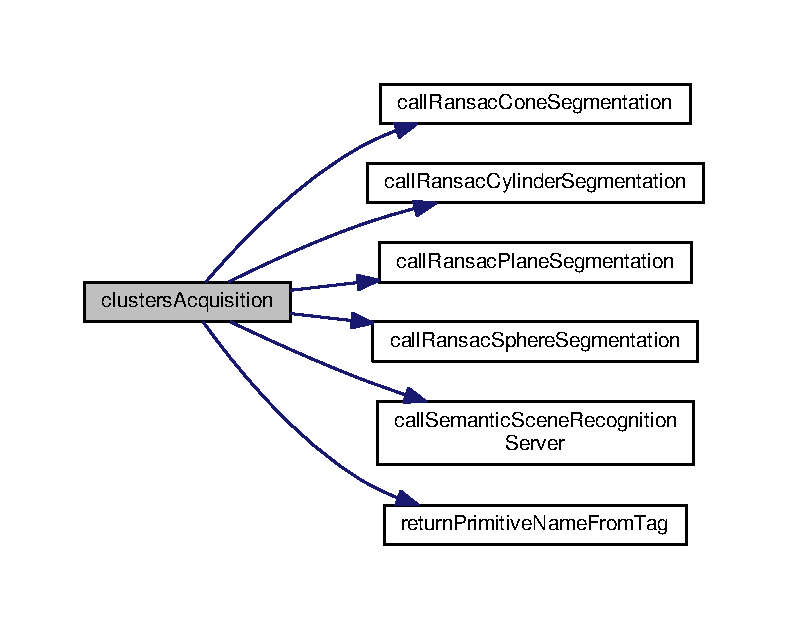
\includegraphics[width=350pt]{ransac__segmentation_8cpp_a87bb87e16486622aae18704555f5af81_cgraph}
\end{center}
\end{figure}


\hypertarget{ransac__segmentation_8cpp_a3c04138a5bfe5d72780bb7e82a18e627}{\index{ransac\-\_\-segmentation.\-cpp@{ransac\-\_\-segmentation.\-cpp}!main@{main}}
\index{main@{main}!ransac_segmentation.cpp@{ransac\-\_\-segmentation.\-cpp}}
\subsubsection[{main}]{\setlength{\rightskip}{0pt plus 5cm}int main (
\begin{DoxyParamCaption}
\item[{int}]{argc, }
\item[{char $\ast$$\ast$}]{argv}
\end{DoxyParamCaption}
)}}\label{ransac__segmentation_8cpp_a3c04138a5bfe5d72780bb7e82a18e627}


Definition at line 402 of file ransac\-\_\-segmentation.\-cpp.



References centroid\-File\-Log, clusters\-Acquisition(), pub, S\-H\-O\-W\-\_\-\-P\-R\-I\-M\-I\-T\-I\-V\-E, and vis.



Here is the call graph for this function\-:\nopagebreak
\begin{figure}[H]
\begin{center}
\leavevmode
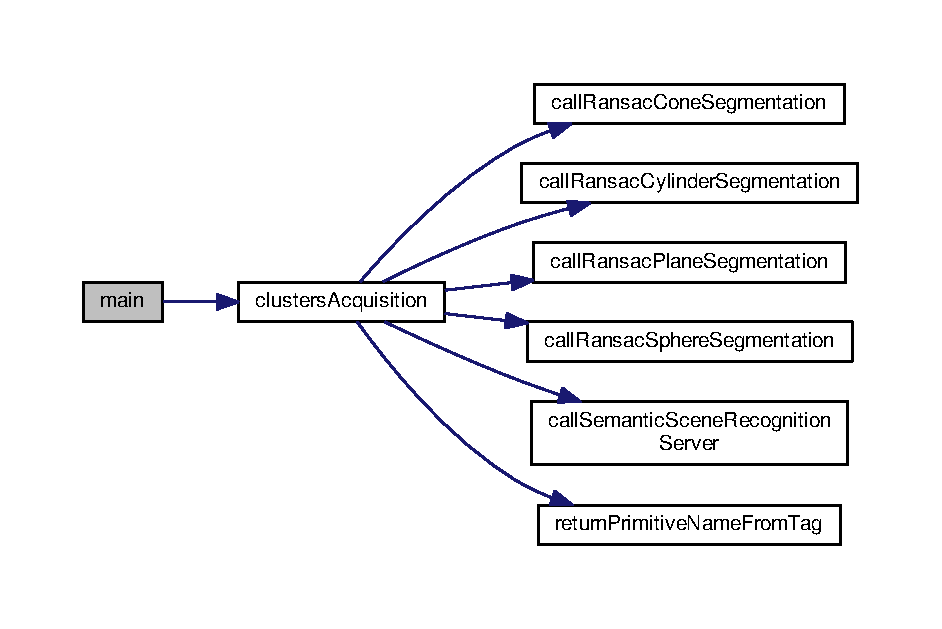
\includegraphics[width=350pt]{ransac__segmentation_8cpp_a3c04138a5bfe5d72780bb7e82a18e627_cgraph}
\end{center}
\end{figure}


\hypertarget{ransac__segmentation_8cpp_a7e84119f095d7369dc280ca585dcd9fb}{\index{ransac\-\_\-segmentation.\-cpp@{ransac\-\_\-segmentation.\-cpp}!print\-Cone\-Info@{print\-Cone\-Info}}
\index{print\-Cone\-Info@{print\-Cone\-Info}!ransac_segmentation.cpp@{ransac\-\_\-segmentation.\-cpp}}
\subsubsection[{print\-Cone\-Info}]{\setlength{\rightskip}{0pt plus 5cm}void print\-Cone\-Info (
\begin{DoxyParamCaption}
\item[{{\bf Primitive\-Segmentation\-Ptr}}]{info, }
\item[{int}]{idx}
\end{DoxyParamCaption}
)}}\label{ransac__segmentation_8cpp_a7e84119f095d7369dc280ca585dcd9fb}


Definition at line 193 of file ransac\-\_\-segmentation.\-cpp.

\hypertarget{ransac__segmentation_8cpp_a45c30fa927c0717d8346839fd1c68bde}{\index{ransac\-\_\-segmentation.\-cpp@{ransac\-\_\-segmentation.\-cpp}!print\-Cylinder\-Info@{print\-Cylinder\-Info}}
\index{print\-Cylinder\-Info@{print\-Cylinder\-Info}!ransac_segmentation.cpp@{ransac\-\_\-segmentation.\-cpp}}
\subsubsection[{print\-Cylinder\-Info}]{\setlength{\rightskip}{0pt plus 5cm}void print\-Cylinder\-Info (
\begin{DoxyParamCaption}
\item[{{\bf Primitive\-Segmentation\-Ptr}}]{info, }
\item[{int}]{idx}
\end{DoxyParamCaption}
)}}\label{ransac__segmentation_8cpp_a45c30fa927c0717d8346839fd1c68bde}


Definition at line 148 of file ransac\-\_\-segmentation.\-cpp.

\hypertarget{ransac__segmentation_8cpp_a20792e9769230baa8e2258731a5143de}{\index{ransac\-\_\-segmentation.\-cpp@{ransac\-\_\-segmentation.\-cpp}!print\-Plane\-Info@{print\-Plane\-Info}}
\index{print\-Plane\-Info@{print\-Plane\-Info}!ransac_segmentation.cpp@{ransac\-\_\-segmentation.\-cpp}}
\subsubsection[{print\-Plane\-Info}]{\setlength{\rightskip}{0pt plus 5cm}void print\-Plane\-Info (
\begin{DoxyParamCaption}
\item[{{\bf Primitive\-Segmentation\-Ptr}}]{info, }
\item[{int}]{idx}
\end{DoxyParamCaption}
)}}\label{ransac__segmentation_8cpp_a20792e9769230baa8e2258731a5143de}


Definition at line 241 of file ransac\-\_\-segmentation.\-cpp.

\hypertarget{ransac__segmentation_8cpp_a575e2f0efaeee850e608ac4481557314}{\index{ransac\-\_\-segmentation.\-cpp@{ransac\-\_\-segmentation.\-cpp}!print\-Sphere\-Info@{print\-Sphere\-Info}}
\index{print\-Sphere\-Info@{print\-Sphere\-Info}!ransac_segmentation.cpp@{ransac\-\_\-segmentation.\-cpp}}
\subsubsection[{print\-Sphere\-Info}]{\setlength{\rightskip}{0pt plus 5cm}void print\-Sphere\-Info (
\begin{DoxyParamCaption}
\item[{{\bf Primitive\-Segmentation\-Ptr}}]{info, }
\item[{int}]{idx}
\end{DoxyParamCaption}
)}}\label{ransac__segmentation_8cpp_a575e2f0efaeee850e608ac4481557314}


Definition at line 105 of file ransac\-\_\-segmentation.\-cpp.

\hypertarget{ransac__segmentation_8cpp_a9fce32945b78e03d2b0abde7198fe623}{\index{ransac\-\_\-segmentation.\-cpp@{ransac\-\_\-segmentation.\-cpp}!return\-Primitive\-Name\-From\-Tag@{return\-Primitive\-Name\-From\-Tag}}
\index{return\-Primitive\-Name\-From\-Tag@{return\-Primitive\-Name\-From\-Tag}!ransac_segmentation.cpp@{ransac\-\_\-segmentation.\-cpp}}
\subsubsection[{return\-Primitive\-Name\-From\-Tag}]{\setlength{\rightskip}{0pt plus 5cm}string return\-Primitive\-Name\-From\-Tag (
\begin{DoxyParamCaption}
\item[{int}]{primitive\-Tag}
\end{DoxyParamCaption}
)}}\label{ransac__segmentation_8cpp_a9fce32945b78e03d2b0abde7198fe623}


Definition at line 250 of file ransac\-\_\-segmentation.\-cpp.



References T\-X\-T\-\_\-\-C\-O\-N\-E\-\_\-\-S\-H\-A\-P\-E\-\_\-\-T\-A\-G, T\-X\-T\-\_\-\-C\-Y\-L\-I\-N\-D\-E\-R\-\_\-\-S\-H\-A\-P\-E\-\_\-\-T\-A\-G, T\-X\-T\-\_\-\-P\-L\-A\-N\-E\-\_\-\-S\-H\-A\-P\-E\-\_\-\-T\-A\-G, T\-X\-T\-\_\-\-S\-P\-H\-E\-R\-E\-\_\-\-S\-H\-A\-P\-E\-\_\-\-T\-A\-G, and T\-X\-T\-\_\-\-U\-N\-K\-N\-O\-W\-N\-\_\-\-S\-H\-A\-P\-E\-\_\-\-T\-A\-G.



Referenced by clusters\-Acquisition().



\subsection{Variable Documentation}
\hypertarget{ransac__segmentation_8cpp_a89794ef3f62d4bfa2dba13649e279e58}{\index{ransac\-\_\-segmentation.\-cpp@{ransac\-\_\-segmentation.\-cpp}!centroid\-File\-Log@{centroid\-File\-Log}}
\index{centroid\-File\-Log@{centroid\-File\-Log}!ransac_segmentation.cpp@{ransac\-\_\-segmentation.\-cpp}}
\subsubsection[{centroid\-File\-Log}]{\setlength{\rightskip}{0pt plus 5cm}string centroid\-File\-Log}}\label{ransac__segmentation_8cpp_a89794ef3f62d4bfa2dba13649e279e58}


Definition at line 283 of file ransac\-\_\-segmentation.\-cpp.



Referenced by main().

\hypertarget{ransac__segmentation_8cpp_a3666640c868c1284aa7cf6787fd149fe}{\index{ransac\-\_\-segmentation.\-cpp@{ransac\-\_\-segmentation.\-cpp}!C\-O\-N\-E\-\_\-\-D\-I\-S\-T\-A\-N\-Z\-E\-\_\-\-T\-H@{C\-O\-N\-E\-\_\-\-D\-I\-S\-T\-A\-N\-Z\-E\-\_\-\-T\-H}}
\index{C\-O\-N\-E\-\_\-\-D\-I\-S\-T\-A\-N\-Z\-E\-\_\-\-T\-H@{C\-O\-N\-E\-\_\-\-D\-I\-S\-T\-A\-N\-Z\-E\-\_\-\-T\-H}!ransac_segmentation.cpp@{ransac\-\_\-segmentation.\-cpp}}
\subsubsection[{C\-O\-N\-E\-\_\-\-D\-I\-S\-T\-A\-N\-Z\-E\-\_\-\-T\-H}]{\setlength{\rightskip}{0pt plus 5cm}const float C\-O\-N\-E\-\_\-\-D\-I\-S\-T\-A\-N\-Z\-E\-\_\-\-T\-H = P\-C\-Manager\-::\-D\-E\-F\-A\-U\-L\-T\-\_\-\-S\-E\-R\-V\-I\-C\-E\-\_\-\-P\-A\-R\-A\-M\-E\-T\-E\-R\-\_\-\-R\-E\-Q\-U\-E\-S\-T\hspace{0.3cm}{\ttfamily [static]}}}\label{ransac__segmentation_8cpp_a3666640c868c1284aa7cf6787fd149fe}


Definition at line 44 of file ransac\-\_\-segmentation.\-cpp.



Referenced by call\-Ransac\-Cone\-Segmentation().

\hypertarget{ransac__segmentation_8cpp_a483dcc255edfca35c9507ac90202f28f}{\index{ransac\-\_\-segmentation.\-cpp@{ransac\-\_\-segmentation.\-cpp}!C\-O\-N\-E\-\_\-\-E\-P\-S\-\_\-\-A\-N\-G\-L\-E\-\_\-\-T\-H@{C\-O\-N\-E\-\_\-\-E\-P\-S\-\_\-\-A\-N\-G\-L\-E\-\_\-\-T\-H}}
\index{C\-O\-N\-E\-\_\-\-E\-P\-S\-\_\-\-A\-N\-G\-L\-E\-\_\-\-T\-H@{C\-O\-N\-E\-\_\-\-E\-P\-S\-\_\-\-A\-N\-G\-L\-E\-\_\-\-T\-H}!ransac_segmentation.cpp@{ransac\-\_\-segmentation.\-cpp}}
\subsubsection[{C\-O\-N\-E\-\_\-\-E\-P\-S\-\_\-\-A\-N\-G\-L\-E\-\_\-\-T\-H}]{\setlength{\rightskip}{0pt plus 5cm}const float C\-O\-N\-E\-\_\-\-E\-P\-S\-\_\-\-A\-N\-G\-L\-E\-\_\-\-T\-H = P\-C\-Manager\-::\-D\-E\-F\-A\-U\-L\-T\-\_\-\-S\-E\-R\-V\-I\-C\-E\-\_\-\-P\-A\-R\-A\-M\-E\-T\-E\-R\-\_\-\-R\-E\-Q\-U\-E\-S\-T\hspace{0.3cm}{\ttfamily [static]}}}\label{ransac__segmentation_8cpp_a483dcc255edfca35c9507ac90202f28f}


Definition at line 48 of file ransac\-\_\-segmentation.\-cpp.



Referenced by call\-Ransac\-Cone\-Segmentation().

\hypertarget{ransac__segmentation_8cpp_af6c0c21521af2937dffda5d2ecf87cf5}{\index{ransac\-\_\-segmentation.\-cpp@{ransac\-\_\-segmentation.\-cpp}!C\-O\-N\-E\-\_\-\-M\-A\-X\-\_\-\-I\-T\-E\-R\-A\-T\-I\-O\-N\-\_\-\-L\-I\-M\-I\-T@{C\-O\-N\-E\-\_\-\-M\-A\-X\-\_\-\-I\-T\-E\-R\-A\-T\-I\-O\-N\-\_\-\-L\-I\-M\-I\-T}}
\index{C\-O\-N\-E\-\_\-\-M\-A\-X\-\_\-\-I\-T\-E\-R\-A\-T\-I\-O\-N\-\_\-\-L\-I\-M\-I\-T@{C\-O\-N\-E\-\_\-\-M\-A\-X\-\_\-\-I\-T\-E\-R\-A\-T\-I\-O\-N\-\_\-\-L\-I\-M\-I\-T}!ransac_segmentation.cpp@{ransac\-\_\-segmentation.\-cpp}}
\subsubsection[{C\-O\-N\-E\-\_\-\-M\-A\-X\-\_\-\-I\-T\-E\-R\-A\-T\-I\-O\-N\-\_\-\-L\-I\-M\-I\-T}]{\setlength{\rightskip}{0pt plus 5cm}const int C\-O\-N\-E\-\_\-\-M\-A\-X\-\_\-\-I\-T\-E\-R\-A\-T\-I\-O\-N\-\_\-\-L\-I\-M\-I\-T = P\-C\-Manager\-::\-D\-E\-F\-A\-U\-L\-T\-\_\-\-S\-E\-R\-V\-I\-C\-E\-\_\-\-P\-A\-R\-A\-M\-E\-T\-E\-R\-\_\-\-R\-E\-Q\-U\-E\-S\-T\hspace{0.3cm}{\ttfamily [static]}}}\label{ransac__segmentation_8cpp_af6c0c21521af2937dffda5d2ecf87cf5}


Definition at line 47 of file ransac\-\_\-segmentation.\-cpp.



Referenced by call\-Ransac\-Cone\-Segmentation().

\hypertarget{ransac__segmentation_8cpp_a82537452866900822ee30a7489259687}{\index{ransac\-\_\-segmentation.\-cpp@{ransac\-\_\-segmentation.\-cpp}!C\-O\-N\-E\-\_\-\-M\-A\-X\-\_\-\-O\-P\-E\-N\-I\-N\-G\-\_\-\-A\-N\-G\-L\-E\-\_\-\-D\-E\-G\-R\-E\-E@{C\-O\-N\-E\-\_\-\-M\-A\-X\-\_\-\-O\-P\-E\-N\-I\-N\-G\-\_\-\-A\-N\-G\-L\-E\-\_\-\-D\-E\-G\-R\-E\-E}}
\index{C\-O\-N\-E\-\_\-\-M\-A\-X\-\_\-\-O\-P\-E\-N\-I\-N\-G\-\_\-\-A\-N\-G\-L\-E\-\_\-\-D\-E\-G\-R\-E\-E@{C\-O\-N\-E\-\_\-\-M\-A\-X\-\_\-\-O\-P\-E\-N\-I\-N\-G\-\_\-\-A\-N\-G\-L\-E\-\_\-\-D\-E\-G\-R\-E\-E}!ransac_segmentation.cpp@{ransac\-\_\-segmentation.\-cpp}}
\subsubsection[{C\-O\-N\-E\-\_\-\-M\-A\-X\-\_\-\-O\-P\-E\-N\-I\-N\-G\-\_\-\-A\-N\-G\-L\-E\-\_\-\-D\-E\-G\-R\-E\-E}]{\setlength{\rightskip}{0pt plus 5cm}const float C\-O\-N\-E\-\_\-\-M\-A\-X\-\_\-\-O\-P\-E\-N\-I\-N\-G\-\_\-\-A\-N\-G\-L\-E\-\_\-\-D\-E\-G\-R\-E\-E = P\-C\-Manager\-::\-D\-E\-F\-A\-U\-L\-T\-\_\-\-S\-E\-R\-V\-I\-C\-E\-\_\-\-P\-A\-R\-A\-M\-E\-T\-E\-R\-\_\-\-R\-E\-Q\-U\-E\-S\-T\hspace{0.3cm}{\ttfamily [static]}}}\label{ransac__segmentation_8cpp_a82537452866900822ee30a7489259687}


Definition at line 50 of file ransac\-\_\-segmentation.\-cpp.



Referenced by call\-Ransac\-Cone\-Segmentation().

\hypertarget{ransac__segmentation_8cpp_a9fc722cbfa5210803b0537e2bbd31a28}{\index{ransac\-\_\-segmentation.\-cpp@{ransac\-\_\-segmentation.\-cpp}!C\-O\-N\-E\-\_\-\-M\-A\-X\-\_\-\-R\-A\-D\-I\-U\-S\-\_\-\-L\-I\-M\-I\-T@{C\-O\-N\-E\-\_\-\-M\-A\-X\-\_\-\-R\-A\-D\-I\-U\-S\-\_\-\-L\-I\-M\-I\-T}}
\index{C\-O\-N\-E\-\_\-\-M\-A\-X\-\_\-\-R\-A\-D\-I\-U\-S\-\_\-\-L\-I\-M\-I\-T@{C\-O\-N\-E\-\_\-\-M\-A\-X\-\_\-\-R\-A\-D\-I\-U\-S\-\_\-\-L\-I\-M\-I\-T}!ransac_segmentation.cpp@{ransac\-\_\-segmentation.\-cpp}}
\subsubsection[{C\-O\-N\-E\-\_\-\-M\-A\-X\-\_\-\-R\-A\-D\-I\-U\-S\-\_\-\-L\-I\-M\-I\-T}]{\setlength{\rightskip}{0pt plus 5cm}const float C\-O\-N\-E\-\_\-\-M\-A\-X\-\_\-\-R\-A\-D\-I\-U\-S\-\_\-\-L\-I\-M\-I\-T = P\-C\-Manager\-::\-D\-E\-F\-A\-U\-L\-T\-\_\-\-S\-E\-R\-V\-I\-C\-E\-\_\-\-P\-A\-R\-A\-M\-E\-T\-E\-R\-\_\-\-R\-E\-Q\-U\-E\-S\-T\hspace{0.3cm}{\ttfamily [static]}}}\label{ransac__segmentation_8cpp_a9fc722cbfa5210803b0537e2bbd31a28}


Definition at line 46 of file ransac\-\_\-segmentation.\-cpp.



Referenced by call\-Ransac\-Cone\-Segmentation().

\hypertarget{ransac__segmentation_8cpp_a5158c226091171a6c24e474c80a97b56}{\index{ransac\-\_\-segmentation.\-cpp@{ransac\-\_\-segmentation.\-cpp}!C\-O\-N\-E\-\_\-\-M\-I\-N\-\_\-\-I\-N\-L\-I\-E\-R\-S@{C\-O\-N\-E\-\_\-\-M\-I\-N\-\_\-\-I\-N\-L\-I\-E\-R\-S}}
\index{C\-O\-N\-E\-\_\-\-M\-I\-N\-\_\-\-I\-N\-L\-I\-E\-R\-S@{C\-O\-N\-E\-\_\-\-M\-I\-N\-\_\-\-I\-N\-L\-I\-E\-R\-S}!ransac_segmentation.cpp@{ransac\-\_\-segmentation.\-cpp}}
\subsubsection[{C\-O\-N\-E\-\_\-\-M\-I\-N\-\_\-\-I\-N\-L\-I\-E\-R\-S}]{\setlength{\rightskip}{0pt plus 5cm}const int C\-O\-N\-E\-\_\-\-M\-I\-N\-\_\-\-I\-N\-L\-I\-E\-R\-S = 40\hspace{0.3cm}{\ttfamily [static]}}}\label{ransac__segmentation_8cpp_a5158c226091171a6c24e474c80a97b56}


Definition at line 51 of file ransac\-\_\-segmentation.\-cpp.



Referenced by call\-Ransac\-Cone\-Segmentation().

\hypertarget{ransac__segmentation_8cpp_a5b31546888827ef9cb72a29d4d519c6d}{\index{ransac\-\_\-segmentation.\-cpp@{ransac\-\_\-segmentation.\-cpp}!C\-O\-N\-E\-\_\-\-M\-I\-N\-\_\-\-O\-P\-E\-N\-I\-N\-G\-\_\-\-A\-N\-G\-L\-E\-\_\-\-D\-E\-G\-R\-E\-E@{C\-O\-N\-E\-\_\-\-M\-I\-N\-\_\-\-O\-P\-E\-N\-I\-N\-G\-\_\-\-A\-N\-G\-L\-E\-\_\-\-D\-E\-G\-R\-E\-E}}
\index{C\-O\-N\-E\-\_\-\-M\-I\-N\-\_\-\-O\-P\-E\-N\-I\-N\-G\-\_\-\-A\-N\-G\-L\-E\-\_\-\-D\-E\-G\-R\-E\-E@{C\-O\-N\-E\-\_\-\-M\-I\-N\-\_\-\-O\-P\-E\-N\-I\-N\-G\-\_\-\-A\-N\-G\-L\-E\-\_\-\-D\-E\-G\-R\-E\-E}!ransac_segmentation.cpp@{ransac\-\_\-segmentation.\-cpp}}
\subsubsection[{C\-O\-N\-E\-\_\-\-M\-I\-N\-\_\-\-O\-P\-E\-N\-I\-N\-G\-\_\-\-A\-N\-G\-L\-E\-\_\-\-D\-E\-G\-R\-E\-E}]{\setlength{\rightskip}{0pt plus 5cm}const float C\-O\-N\-E\-\_\-\-M\-I\-N\-\_\-\-O\-P\-E\-N\-I\-N\-G\-\_\-\-A\-N\-G\-L\-E\-\_\-\-D\-E\-G\-R\-E\-E = P\-C\-Manager\-::\-D\-E\-F\-A\-U\-L\-T\-\_\-\-S\-E\-R\-V\-I\-C\-E\-\_\-\-P\-A\-R\-A\-M\-E\-T\-E\-R\-\_\-\-R\-E\-Q\-U\-E\-S\-T\hspace{0.3cm}{\ttfamily [static]}}}\label{ransac__segmentation_8cpp_a5b31546888827ef9cb72a29d4d519c6d}


Definition at line 49 of file ransac\-\_\-segmentation.\-cpp.



Referenced by call\-Ransac\-Cone\-Segmentation().

\hypertarget{ransac__segmentation_8cpp_a439b350e5c68e7217f00d1c8f556d635}{\index{ransac\-\_\-segmentation.\-cpp@{ransac\-\_\-segmentation.\-cpp}!C\-O\-N\-E\-\_\-\-M\-I\-N\-\_\-\-R\-A\-D\-I\-U\-S\-\_\-\-L\-I\-M\-I\-T@{C\-O\-N\-E\-\_\-\-M\-I\-N\-\_\-\-R\-A\-D\-I\-U\-S\-\_\-\-L\-I\-M\-I\-T}}
\index{C\-O\-N\-E\-\_\-\-M\-I\-N\-\_\-\-R\-A\-D\-I\-U\-S\-\_\-\-L\-I\-M\-I\-T@{C\-O\-N\-E\-\_\-\-M\-I\-N\-\_\-\-R\-A\-D\-I\-U\-S\-\_\-\-L\-I\-M\-I\-T}!ransac_segmentation.cpp@{ransac\-\_\-segmentation.\-cpp}}
\subsubsection[{C\-O\-N\-E\-\_\-\-M\-I\-N\-\_\-\-R\-A\-D\-I\-U\-S\-\_\-\-L\-I\-M\-I\-T}]{\setlength{\rightskip}{0pt plus 5cm}const float C\-O\-N\-E\-\_\-\-M\-I\-N\-\_\-\-R\-A\-D\-I\-U\-S\-\_\-\-L\-I\-M\-I\-T = P\-C\-Manager\-::\-D\-E\-F\-A\-U\-L\-T\-\_\-\-S\-E\-R\-V\-I\-C\-E\-\_\-\-P\-A\-R\-A\-M\-E\-T\-E\-R\-\_\-\-R\-E\-Q\-U\-E\-S\-T\hspace{0.3cm}{\ttfamily [static]}}}\label{ransac__segmentation_8cpp_a439b350e5c68e7217f00d1c8f556d635}


Definition at line 45 of file ransac\-\_\-segmentation.\-cpp.



Referenced by call\-Ransac\-Cone\-Segmentation().

\hypertarget{ransac__segmentation_8cpp_a88820a487e8ea05a5ace76f7da623c4d}{\index{ransac\-\_\-segmentation.\-cpp@{ransac\-\_\-segmentation.\-cpp}!C\-O\-N\-E\-\_\-\-N\-O\-R\-M\-A\-L\-\_\-\-D\-I\-S\-T\-A\-N\-C\-E\-\_\-\-W\-E\-I\-G\-T\-H@{C\-O\-N\-E\-\_\-\-N\-O\-R\-M\-A\-L\-\_\-\-D\-I\-S\-T\-A\-N\-C\-E\-\_\-\-W\-E\-I\-G\-T\-H}}
\index{C\-O\-N\-E\-\_\-\-N\-O\-R\-M\-A\-L\-\_\-\-D\-I\-S\-T\-A\-N\-C\-E\-\_\-\-W\-E\-I\-G\-T\-H@{C\-O\-N\-E\-\_\-\-N\-O\-R\-M\-A\-L\-\_\-\-D\-I\-S\-T\-A\-N\-C\-E\-\_\-\-W\-E\-I\-G\-T\-H}!ransac_segmentation.cpp@{ransac\-\_\-segmentation.\-cpp}}
\subsubsection[{C\-O\-N\-E\-\_\-\-N\-O\-R\-M\-A\-L\-\_\-\-D\-I\-S\-T\-A\-N\-C\-E\-\_\-\-W\-E\-I\-G\-T\-H}]{\setlength{\rightskip}{0pt plus 5cm}const float C\-O\-N\-E\-\_\-\-N\-O\-R\-M\-A\-L\-\_\-\-D\-I\-S\-T\-A\-N\-C\-E\-\_\-\-W\-E\-I\-G\-T\-H = P\-C\-Manager\-::\-D\-E\-F\-A\-U\-L\-T\-\_\-\-S\-E\-R\-V\-I\-C\-E\-\_\-\-P\-A\-R\-A\-M\-E\-T\-E\-R\-\_\-\-R\-E\-Q\-U\-E\-S\-T\hspace{0.3cm}{\ttfamily [static]}}}\label{ransac__segmentation_8cpp_a88820a487e8ea05a5ace76f7da623c4d}


Definition at line 43 of file ransac\-\_\-segmentation.\-cpp.



Referenced by call\-Ransac\-Cone\-Segmentation().

\hypertarget{ransac__segmentation_8cpp_a88890b57d71f10e081848a98e9a74b54}{\index{ransac\-\_\-segmentation.\-cpp@{ransac\-\_\-segmentation.\-cpp}!C\-O\-N\-E\-\_\-\-T\-O\-\_\-\-C\-Y\-L\-I\-N\-D\-E\-R\-\_\-\-P\-R\-I\-O\-R\-I\-T\-Y@{C\-O\-N\-E\-\_\-\-T\-O\-\_\-\-C\-Y\-L\-I\-N\-D\-E\-R\-\_\-\-P\-R\-I\-O\-R\-I\-T\-Y}}
\index{C\-O\-N\-E\-\_\-\-T\-O\-\_\-\-C\-Y\-L\-I\-N\-D\-E\-R\-\_\-\-P\-R\-I\-O\-R\-I\-T\-Y@{C\-O\-N\-E\-\_\-\-T\-O\-\_\-\-C\-Y\-L\-I\-N\-D\-E\-R\-\_\-\-P\-R\-I\-O\-R\-I\-T\-Y}!ransac_segmentation.cpp@{ransac\-\_\-segmentation.\-cpp}}
\subsubsection[{C\-O\-N\-E\-\_\-\-T\-O\-\_\-\-C\-Y\-L\-I\-N\-D\-E\-R\-\_\-\-P\-R\-I\-O\-R\-I\-T\-Y}]{\setlength{\rightskip}{0pt plus 5cm}const float C\-O\-N\-E\-\_\-\-T\-O\-\_\-\-C\-Y\-L\-I\-N\-D\-E\-R\-\_\-\-P\-R\-I\-O\-R\-I\-T\-Y = 0.\-9f\hspace{0.3cm}{\ttfamily [static]}}}\label{ransac__segmentation_8cpp_a88890b57d71f10e081848a98e9a74b54}


Definition at line 64 of file ransac\-\_\-segmentation.\-cpp.



Referenced by clusters\-Acquisition().

\hypertarget{ransac__segmentation_8cpp_a1668124b29d98531885609eb11ef7c01}{\index{ransac\-\_\-segmentation.\-cpp@{ransac\-\_\-segmentation.\-cpp}!C\-Y\-L\-I\-N\-D\-E\-R\-\_\-\-D\-I\-S\-T\-A\-N\-Z\-E\-\_\-\-T\-H@{C\-Y\-L\-I\-N\-D\-E\-R\-\_\-\-D\-I\-S\-T\-A\-N\-Z\-E\-\_\-\-T\-H}}
\index{C\-Y\-L\-I\-N\-D\-E\-R\-\_\-\-D\-I\-S\-T\-A\-N\-Z\-E\-\_\-\-T\-H@{C\-Y\-L\-I\-N\-D\-E\-R\-\_\-\-D\-I\-S\-T\-A\-N\-Z\-E\-\_\-\-T\-H}!ransac_segmentation.cpp@{ransac\-\_\-segmentation.\-cpp}}
\subsubsection[{C\-Y\-L\-I\-N\-D\-E\-R\-\_\-\-D\-I\-S\-T\-A\-N\-Z\-E\-\_\-\-T\-H}]{\setlength{\rightskip}{0pt plus 5cm}const float C\-Y\-L\-I\-N\-D\-E\-R\-\_\-\-D\-I\-S\-T\-A\-N\-Z\-E\-\_\-\-T\-H = P\-C\-Manager\-::\-D\-E\-F\-A\-U\-L\-T\-\_\-\-S\-E\-R\-V\-I\-C\-E\-\_\-\-P\-A\-R\-A\-M\-E\-T\-E\-R\-\_\-\-R\-E\-Q\-U\-E\-S\-T\hspace{0.3cm}{\ttfamily [static]}}}\label{ransac__segmentation_8cpp_a1668124b29d98531885609eb11ef7c01}


Definition at line 34 of file ransac\-\_\-segmentation.\-cpp.



Referenced by call\-Ransac\-Cylinder\-Segmentation().

\hypertarget{ransac__segmentation_8cpp_a43836ff1ad6b5443b700ce7d8f7f3894}{\index{ransac\-\_\-segmentation.\-cpp@{ransac\-\_\-segmentation.\-cpp}!C\-Y\-L\-I\-N\-D\-E\-R\-\_\-\-E\-P\-S\-\_\-\-A\-N\-G\-L\-E\-\_\-\-T\-H@{C\-Y\-L\-I\-N\-D\-E\-R\-\_\-\-E\-P\-S\-\_\-\-A\-N\-G\-L\-E\-\_\-\-T\-H}}
\index{C\-Y\-L\-I\-N\-D\-E\-R\-\_\-\-E\-P\-S\-\_\-\-A\-N\-G\-L\-E\-\_\-\-T\-H@{C\-Y\-L\-I\-N\-D\-E\-R\-\_\-\-E\-P\-S\-\_\-\-A\-N\-G\-L\-E\-\_\-\-T\-H}!ransac_segmentation.cpp@{ransac\-\_\-segmentation.\-cpp}}
\subsubsection[{C\-Y\-L\-I\-N\-D\-E\-R\-\_\-\-E\-P\-S\-\_\-\-A\-N\-G\-L\-E\-\_\-\-T\-H}]{\setlength{\rightskip}{0pt plus 5cm}const float C\-Y\-L\-I\-N\-D\-E\-R\-\_\-\-E\-P\-S\-\_\-\-A\-N\-G\-L\-E\-\_\-\-T\-H = P\-C\-Manager\-::\-D\-E\-F\-A\-U\-L\-T\-\_\-\-S\-E\-R\-V\-I\-C\-E\-\_\-\-P\-A\-R\-A\-M\-E\-T\-E\-R\-\_\-\-R\-E\-Q\-U\-E\-S\-T\hspace{0.3cm}{\ttfamily [static]}}}\label{ransac__segmentation_8cpp_a43836ff1ad6b5443b700ce7d8f7f3894}


Definition at line 38 of file ransac\-\_\-segmentation.\-cpp.



Referenced by call\-Ransac\-Cylinder\-Segmentation().

\hypertarget{ransac__segmentation_8cpp_adcc696ebb221c4d1cbfc378ccb7e705d}{\index{ransac\-\_\-segmentation.\-cpp@{ransac\-\_\-segmentation.\-cpp}!C\-Y\-L\-I\-N\-D\-E\-R\-\_\-\-M\-A\-X\-\_\-\-I\-T\-E\-R\-A\-T\-I\-O\-N\-\_\-\-L\-I\-M\-I\-T@{C\-Y\-L\-I\-N\-D\-E\-R\-\_\-\-M\-A\-X\-\_\-\-I\-T\-E\-R\-A\-T\-I\-O\-N\-\_\-\-L\-I\-M\-I\-T}}
\index{C\-Y\-L\-I\-N\-D\-E\-R\-\_\-\-M\-A\-X\-\_\-\-I\-T\-E\-R\-A\-T\-I\-O\-N\-\_\-\-L\-I\-M\-I\-T@{C\-Y\-L\-I\-N\-D\-E\-R\-\_\-\-M\-A\-X\-\_\-\-I\-T\-E\-R\-A\-T\-I\-O\-N\-\_\-\-L\-I\-M\-I\-T}!ransac_segmentation.cpp@{ransac\-\_\-segmentation.\-cpp}}
\subsubsection[{C\-Y\-L\-I\-N\-D\-E\-R\-\_\-\-M\-A\-X\-\_\-\-I\-T\-E\-R\-A\-T\-I\-O\-N\-\_\-\-L\-I\-M\-I\-T}]{\setlength{\rightskip}{0pt plus 5cm}const int C\-Y\-L\-I\-N\-D\-E\-R\-\_\-\-M\-A\-X\-\_\-\-I\-T\-E\-R\-A\-T\-I\-O\-N\-\_\-\-L\-I\-M\-I\-T = P\-C\-Manager\-::\-D\-E\-F\-A\-U\-L\-T\-\_\-\-S\-E\-R\-V\-I\-C\-E\-\_\-\-P\-A\-R\-A\-M\-E\-T\-E\-R\-\_\-\-R\-E\-Q\-U\-E\-S\-T\hspace{0.3cm}{\ttfamily [static]}}}\label{ransac__segmentation_8cpp_adcc696ebb221c4d1cbfc378ccb7e705d}


Definition at line 37 of file ransac\-\_\-segmentation.\-cpp.



Referenced by call\-Ransac\-Cylinder\-Segmentation().

\hypertarget{ransac__segmentation_8cpp_a305b62f577d4441065ced776ec99c81c}{\index{ransac\-\_\-segmentation.\-cpp@{ransac\-\_\-segmentation.\-cpp}!C\-Y\-L\-I\-N\-D\-E\-R\-\_\-\-M\-A\-X\-\_\-\-O\-P\-E\-N\-I\-N\-G\-\_\-\-A\-N\-G\-L\-E\-\_\-\-D\-E\-G\-R\-E\-E@{C\-Y\-L\-I\-N\-D\-E\-R\-\_\-\-M\-A\-X\-\_\-\-O\-P\-E\-N\-I\-N\-G\-\_\-\-A\-N\-G\-L\-E\-\_\-\-D\-E\-G\-R\-E\-E}}
\index{C\-Y\-L\-I\-N\-D\-E\-R\-\_\-\-M\-A\-X\-\_\-\-O\-P\-E\-N\-I\-N\-G\-\_\-\-A\-N\-G\-L\-E\-\_\-\-D\-E\-G\-R\-E\-E@{C\-Y\-L\-I\-N\-D\-E\-R\-\_\-\-M\-A\-X\-\_\-\-O\-P\-E\-N\-I\-N\-G\-\_\-\-A\-N\-G\-L\-E\-\_\-\-D\-E\-G\-R\-E\-E}!ransac_segmentation.cpp@{ransac\-\_\-segmentation.\-cpp}}
\subsubsection[{C\-Y\-L\-I\-N\-D\-E\-R\-\_\-\-M\-A\-X\-\_\-\-O\-P\-E\-N\-I\-N\-G\-\_\-\-A\-N\-G\-L\-E\-\_\-\-D\-E\-G\-R\-E\-E}]{\setlength{\rightskip}{0pt plus 5cm}const float C\-Y\-L\-I\-N\-D\-E\-R\-\_\-\-M\-A\-X\-\_\-\-O\-P\-E\-N\-I\-N\-G\-\_\-\-A\-N\-G\-L\-E\-\_\-\-D\-E\-G\-R\-E\-E = P\-C\-Manager\-::\-D\-E\-F\-A\-U\-L\-T\-\_\-\-S\-E\-R\-V\-I\-C\-E\-\_\-\-P\-A\-R\-A\-M\-E\-T\-E\-R\-\_\-\-R\-E\-Q\-U\-E\-S\-T\hspace{0.3cm}{\ttfamily [static]}}}\label{ransac__segmentation_8cpp_a305b62f577d4441065ced776ec99c81c}


Definition at line 40 of file ransac\-\_\-segmentation.\-cpp.



Referenced by call\-Ransac\-Cylinder\-Segmentation().

\hypertarget{ransac__segmentation_8cpp_a7eb55fccf674572aa0b48f47ff780b3b}{\index{ransac\-\_\-segmentation.\-cpp@{ransac\-\_\-segmentation.\-cpp}!C\-Y\-L\-I\-N\-D\-E\-R\-\_\-\-M\-A\-X\-\_\-\-R\-A\-D\-I\-U\-S\-\_\-\-L\-I\-M\-I\-T@{C\-Y\-L\-I\-N\-D\-E\-R\-\_\-\-M\-A\-X\-\_\-\-R\-A\-D\-I\-U\-S\-\_\-\-L\-I\-M\-I\-T}}
\index{C\-Y\-L\-I\-N\-D\-E\-R\-\_\-\-M\-A\-X\-\_\-\-R\-A\-D\-I\-U\-S\-\_\-\-L\-I\-M\-I\-T@{C\-Y\-L\-I\-N\-D\-E\-R\-\_\-\-M\-A\-X\-\_\-\-R\-A\-D\-I\-U\-S\-\_\-\-L\-I\-M\-I\-T}!ransac_segmentation.cpp@{ransac\-\_\-segmentation.\-cpp}}
\subsubsection[{C\-Y\-L\-I\-N\-D\-E\-R\-\_\-\-M\-A\-X\-\_\-\-R\-A\-D\-I\-U\-S\-\_\-\-L\-I\-M\-I\-T}]{\setlength{\rightskip}{0pt plus 5cm}const float C\-Y\-L\-I\-N\-D\-E\-R\-\_\-\-M\-A\-X\-\_\-\-R\-A\-D\-I\-U\-S\-\_\-\-L\-I\-M\-I\-T = P\-C\-Manager\-::\-D\-E\-F\-A\-U\-L\-T\-\_\-\-S\-E\-R\-V\-I\-C\-E\-\_\-\-P\-A\-R\-A\-M\-E\-T\-E\-R\-\_\-\-R\-E\-Q\-U\-E\-S\-T\hspace{0.3cm}{\ttfamily [static]}}}\label{ransac__segmentation_8cpp_a7eb55fccf674572aa0b48f47ff780b3b}


Definition at line 36 of file ransac\-\_\-segmentation.\-cpp.



Referenced by call\-Ransac\-Cylinder\-Segmentation().

\hypertarget{ransac__segmentation_8cpp_a88e5139f490ddafb49b07a61ca7bbabf}{\index{ransac\-\_\-segmentation.\-cpp@{ransac\-\_\-segmentation.\-cpp}!C\-Y\-L\-I\-N\-D\-E\-R\-\_\-\-M\-I\-N\-\_\-\-I\-N\-L\-I\-E\-R\-S@{C\-Y\-L\-I\-N\-D\-E\-R\-\_\-\-M\-I\-N\-\_\-\-I\-N\-L\-I\-E\-R\-S}}
\index{C\-Y\-L\-I\-N\-D\-E\-R\-\_\-\-M\-I\-N\-\_\-\-I\-N\-L\-I\-E\-R\-S@{C\-Y\-L\-I\-N\-D\-E\-R\-\_\-\-M\-I\-N\-\_\-\-I\-N\-L\-I\-E\-R\-S}!ransac_segmentation.cpp@{ransac\-\_\-segmentation.\-cpp}}
\subsubsection[{C\-Y\-L\-I\-N\-D\-E\-R\-\_\-\-M\-I\-N\-\_\-\-I\-N\-L\-I\-E\-R\-S}]{\setlength{\rightskip}{0pt plus 5cm}const int C\-Y\-L\-I\-N\-D\-E\-R\-\_\-\-M\-I\-N\-\_\-\-I\-N\-L\-I\-E\-R\-S = 40\hspace{0.3cm}{\ttfamily [static]}}}\label{ransac__segmentation_8cpp_a88e5139f490ddafb49b07a61ca7bbabf}


Definition at line 41 of file ransac\-\_\-segmentation.\-cpp.



Referenced by call\-Ransac\-Cylinder\-Segmentation().

\hypertarget{ransac__segmentation_8cpp_ab86c6010ac83848f660f9e1d0323a3a6}{\index{ransac\-\_\-segmentation.\-cpp@{ransac\-\_\-segmentation.\-cpp}!C\-Y\-L\-I\-N\-D\-E\-R\-\_\-\-M\-I\-N\-\_\-\-O\-P\-E\-N\-I\-N\-G\-\_\-\-A\-N\-G\-L\-E\-\_\-\-D\-E\-G\-R\-E\-E@{C\-Y\-L\-I\-N\-D\-E\-R\-\_\-\-M\-I\-N\-\_\-\-O\-P\-E\-N\-I\-N\-G\-\_\-\-A\-N\-G\-L\-E\-\_\-\-D\-E\-G\-R\-E\-E}}
\index{C\-Y\-L\-I\-N\-D\-E\-R\-\_\-\-M\-I\-N\-\_\-\-O\-P\-E\-N\-I\-N\-G\-\_\-\-A\-N\-G\-L\-E\-\_\-\-D\-E\-G\-R\-E\-E@{C\-Y\-L\-I\-N\-D\-E\-R\-\_\-\-M\-I\-N\-\_\-\-O\-P\-E\-N\-I\-N\-G\-\_\-\-A\-N\-G\-L\-E\-\_\-\-D\-E\-G\-R\-E\-E}!ransac_segmentation.cpp@{ransac\-\_\-segmentation.\-cpp}}
\subsubsection[{C\-Y\-L\-I\-N\-D\-E\-R\-\_\-\-M\-I\-N\-\_\-\-O\-P\-E\-N\-I\-N\-G\-\_\-\-A\-N\-G\-L\-E\-\_\-\-D\-E\-G\-R\-E\-E}]{\setlength{\rightskip}{0pt plus 5cm}const float C\-Y\-L\-I\-N\-D\-E\-R\-\_\-\-M\-I\-N\-\_\-\-O\-P\-E\-N\-I\-N\-G\-\_\-\-A\-N\-G\-L\-E\-\_\-\-D\-E\-G\-R\-E\-E = P\-C\-Manager\-::\-D\-E\-F\-A\-U\-L\-T\-\_\-\-S\-E\-R\-V\-I\-C\-E\-\_\-\-P\-A\-R\-A\-M\-E\-T\-E\-R\-\_\-\-R\-E\-Q\-U\-E\-S\-T\hspace{0.3cm}{\ttfamily [static]}}}\label{ransac__segmentation_8cpp_ab86c6010ac83848f660f9e1d0323a3a6}


Definition at line 39 of file ransac\-\_\-segmentation.\-cpp.



Referenced by call\-Ransac\-Cylinder\-Segmentation().

\hypertarget{ransac__segmentation_8cpp_a0c4f9fd70b994784fd2c8b8b85f83d2a}{\index{ransac\-\_\-segmentation.\-cpp@{ransac\-\_\-segmentation.\-cpp}!C\-Y\-L\-I\-N\-D\-E\-R\-\_\-\-M\-I\-N\-\_\-\-R\-A\-D\-I\-U\-S\-\_\-\-L\-I\-M\-I\-T@{C\-Y\-L\-I\-N\-D\-E\-R\-\_\-\-M\-I\-N\-\_\-\-R\-A\-D\-I\-U\-S\-\_\-\-L\-I\-M\-I\-T}}
\index{C\-Y\-L\-I\-N\-D\-E\-R\-\_\-\-M\-I\-N\-\_\-\-R\-A\-D\-I\-U\-S\-\_\-\-L\-I\-M\-I\-T@{C\-Y\-L\-I\-N\-D\-E\-R\-\_\-\-M\-I\-N\-\_\-\-R\-A\-D\-I\-U\-S\-\_\-\-L\-I\-M\-I\-T}!ransac_segmentation.cpp@{ransac\-\_\-segmentation.\-cpp}}
\subsubsection[{C\-Y\-L\-I\-N\-D\-E\-R\-\_\-\-M\-I\-N\-\_\-\-R\-A\-D\-I\-U\-S\-\_\-\-L\-I\-M\-I\-T}]{\setlength{\rightskip}{0pt plus 5cm}const float C\-Y\-L\-I\-N\-D\-E\-R\-\_\-\-M\-I\-N\-\_\-\-R\-A\-D\-I\-U\-S\-\_\-\-L\-I\-M\-I\-T = P\-C\-Manager\-::\-D\-E\-F\-A\-U\-L\-T\-\_\-\-S\-E\-R\-V\-I\-C\-E\-\_\-\-P\-A\-R\-A\-M\-E\-T\-E\-R\-\_\-\-R\-E\-Q\-U\-E\-S\-T\hspace{0.3cm}{\ttfamily [static]}}}\label{ransac__segmentation_8cpp_a0c4f9fd70b994784fd2c8b8b85f83d2a}


Definition at line 35 of file ransac\-\_\-segmentation.\-cpp.



Referenced by call\-Ransac\-Cylinder\-Segmentation().

\hypertarget{ransac__segmentation_8cpp_a343ca34ce396f1e85c6e4c76889006ad}{\index{ransac\-\_\-segmentation.\-cpp@{ransac\-\_\-segmentation.\-cpp}!C\-Y\-L\-I\-N\-D\-E\-R\-\_\-\-N\-O\-R\-M\-A\-L\-\_\-\-D\-I\-S\-T\-A\-N\-C\-E\-\_\-\-W\-E\-I\-G\-T\-H@{C\-Y\-L\-I\-N\-D\-E\-R\-\_\-\-N\-O\-R\-M\-A\-L\-\_\-\-D\-I\-S\-T\-A\-N\-C\-E\-\_\-\-W\-E\-I\-G\-T\-H}}
\index{C\-Y\-L\-I\-N\-D\-E\-R\-\_\-\-N\-O\-R\-M\-A\-L\-\_\-\-D\-I\-S\-T\-A\-N\-C\-E\-\_\-\-W\-E\-I\-G\-T\-H@{C\-Y\-L\-I\-N\-D\-E\-R\-\_\-\-N\-O\-R\-M\-A\-L\-\_\-\-D\-I\-S\-T\-A\-N\-C\-E\-\_\-\-W\-E\-I\-G\-T\-H}!ransac_segmentation.cpp@{ransac\-\_\-segmentation.\-cpp}}
\subsubsection[{C\-Y\-L\-I\-N\-D\-E\-R\-\_\-\-N\-O\-R\-M\-A\-L\-\_\-\-D\-I\-S\-T\-A\-N\-C\-E\-\_\-\-W\-E\-I\-G\-T\-H}]{\setlength{\rightskip}{0pt plus 5cm}const float C\-Y\-L\-I\-N\-D\-E\-R\-\_\-\-N\-O\-R\-M\-A\-L\-\_\-\-D\-I\-S\-T\-A\-N\-C\-E\-\_\-\-W\-E\-I\-G\-T\-H = P\-C\-Manager\-::\-D\-E\-F\-A\-U\-L\-T\-\_\-\-S\-E\-R\-V\-I\-C\-E\-\_\-\-P\-A\-R\-A\-M\-E\-T\-E\-R\-\_\-\-R\-E\-Q\-U\-E\-S\-T\hspace{0.3cm}{\ttfamily [static]}}}\label{ransac__segmentation_8cpp_a343ca34ce396f1e85c6e4c76889006ad}


Definition at line 33 of file ransac\-\_\-segmentation.\-cpp.



Referenced by call\-Ransac\-Cylinder\-Segmentation().

\hypertarget{ransac__segmentation_8cpp_a44459fc7aff832a1bbfbe33684eb7b3b}{\index{ransac\-\_\-segmentation.\-cpp@{ransac\-\_\-segmentation.\-cpp}!P\-L\-A\-N\-E\-\_\-\-D\-I\-S\-T\-A\-N\-Z\-E\-\_\-\-T\-H@{P\-L\-A\-N\-E\-\_\-\-D\-I\-S\-T\-A\-N\-Z\-E\-\_\-\-T\-H}}
\index{P\-L\-A\-N\-E\-\_\-\-D\-I\-S\-T\-A\-N\-Z\-E\-\_\-\-T\-H@{P\-L\-A\-N\-E\-\_\-\-D\-I\-S\-T\-A\-N\-Z\-E\-\_\-\-T\-H}!ransac_segmentation.cpp@{ransac\-\_\-segmentation.\-cpp}}
\subsubsection[{P\-L\-A\-N\-E\-\_\-\-D\-I\-S\-T\-A\-N\-Z\-E\-\_\-\-T\-H}]{\setlength{\rightskip}{0pt plus 5cm}const float P\-L\-A\-N\-E\-\_\-\-D\-I\-S\-T\-A\-N\-Z\-E\-\_\-\-T\-H = P\-C\-Manager\-::\-D\-E\-F\-A\-U\-L\-T\-\_\-\-S\-E\-R\-V\-I\-C\-E\-\_\-\-P\-A\-R\-A\-M\-E\-T\-E\-R\-\_\-\-R\-E\-Q\-U\-E\-S\-T\hspace{0.3cm}{\ttfamily [static]}}}\label{ransac__segmentation_8cpp_a44459fc7aff832a1bbfbe33684eb7b3b}


Definition at line 54 of file ransac\-\_\-segmentation.\-cpp.



Referenced by call\-Ransac\-Plane\-Segmentation().

\hypertarget{ransac__segmentation_8cpp_a202ce91ef6bc7696022ae0b652df88ca}{\index{ransac\-\_\-segmentation.\-cpp@{ransac\-\_\-segmentation.\-cpp}!P\-L\-A\-N\-E\-\_\-\-E\-P\-S\-\_\-\-A\-N\-G\-L\-E\-\_\-\-T\-H@{P\-L\-A\-N\-E\-\_\-\-E\-P\-S\-\_\-\-A\-N\-G\-L\-E\-\_\-\-T\-H}}
\index{P\-L\-A\-N\-E\-\_\-\-E\-P\-S\-\_\-\-A\-N\-G\-L\-E\-\_\-\-T\-H@{P\-L\-A\-N\-E\-\_\-\-E\-P\-S\-\_\-\-A\-N\-G\-L\-E\-\_\-\-T\-H}!ransac_segmentation.cpp@{ransac\-\_\-segmentation.\-cpp}}
\subsubsection[{P\-L\-A\-N\-E\-\_\-\-E\-P\-S\-\_\-\-A\-N\-G\-L\-E\-\_\-\-T\-H}]{\setlength{\rightskip}{0pt plus 5cm}const float P\-L\-A\-N\-E\-\_\-\-E\-P\-S\-\_\-\-A\-N\-G\-L\-E\-\_\-\-T\-H = P\-C\-Manager\-::\-D\-E\-F\-A\-U\-L\-T\-\_\-\-S\-E\-R\-V\-I\-C\-E\-\_\-\-P\-A\-R\-A\-M\-E\-T\-E\-R\-\_\-\-R\-E\-Q\-U\-E\-S\-T\hspace{0.3cm}{\ttfamily [static]}}}\label{ransac__segmentation_8cpp_a202ce91ef6bc7696022ae0b652df88ca}


Definition at line 58 of file ransac\-\_\-segmentation.\-cpp.



Referenced by call\-Ransac\-Plane\-Segmentation().

\hypertarget{ransac__segmentation_8cpp_a6af34946e4b18e3262d6c8c3df454d41}{\index{ransac\-\_\-segmentation.\-cpp@{ransac\-\_\-segmentation.\-cpp}!P\-L\-A\-N\-E\-\_\-\-M\-A\-X\-\_\-\-I\-T\-E\-R\-A\-T\-I\-O\-N\-\_\-\-L\-I\-M\-I\-T@{P\-L\-A\-N\-E\-\_\-\-M\-A\-X\-\_\-\-I\-T\-E\-R\-A\-T\-I\-O\-N\-\_\-\-L\-I\-M\-I\-T}}
\index{P\-L\-A\-N\-E\-\_\-\-M\-A\-X\-\_\-\-I\-T\-E\-R\-A\-T\-I\-O\-N\-\_\-\-L\-I\-M\-I\-T@{P\-L\-A\-N\-E\-\_\-\-M\-A\-X\-\_\-\-I\-T\-E\-R\-A\-T\-I\-O\-N\-\_\-\-L\-I\-M\-I\-T}!ransac_segmentation.cpp@{ransac\-\_\-segmentation.\-cpp}}
\subsubsection[{P\-L\-A\-N\-E\-\_\-\-M\-A\-X\-\_\-\-I\-T\-E\-R\-A\-T\-I\-O\-N\-\_\-\-L\-I\-M\-I\-T}]{\setlength{\rightskip}{0pt plus 5cm}const int P\-L\-A\-N\-E\-\_\-\-M\-A\-X\-\_\-\-I\-T\-E\-R\-A\-T\-I\-O\-N\-\_\-\-L\-I\-M\-I\-T = P\-C\-Manager\-::\-D\-E\-F\-A\-U\-L\-T\-\_\-\-S\-E\-R\-V\-I\-C\-E\-\_\-\-P\-A\-R\-A\-M\-E\-T\-E\-R\-\_\-\-R\-E\-Q\-U\-E\-S\-T\hspace{0.3cm}{\ttfamily [static]}}}\label{ransac__segmentation_8cpp_a6af34946e4b18e3262d6c8c3df454d41}


Definition at line 57 of file ransac\-\_\-segmentation.\-cpp.



Referenced by call\-Ransac\-Plane\-Segmentation().

\hypertarget{ransac__segmentation_8cpp_a2c44becf927c6208a0880f8bea4ee70d}{\index{ransac\-\_\-segmentation.\-cpp@{ransac\-\_\-segmentation.\-cpp}!P\-L\-A\-N\-E\-\_\-\-M\-A\-X\-\_\-\-O\-P\-E\-N\-I\-N\-G\-\_\-\-A\-N\-G\-L\-E\-\_\-\-D\-E\-G\-R\-E\-E@{P\-L\-A\-N\-E\-\_\-\-M\-A\-X\-\_\-\-O\-P\-E\-N\-I\-N\-G\-\_\-\-A\-N\-G\-L\-E\-\_\-\-D\-E\-G\-R\-E\-E}}
\index{P\-L\-A\-N\-E\-\_\-\-M\-A\-X\-\_\-\-O\-P\-E\-N\-I\-N\-G\-\_\-\-A\-N\-G\-L\-E\-\_\-\-D\-E\-G\-R\-E\-E@{P\-L\-A\-N\-E\-\_\-\-M\-A\-X\-\_\-\-O\-P\-E\-N\-I\-N\-G\-\_\-\-A\-N\-G\-L\-E\-\_\-\-D\-E\-G\-R\-E\-E}!ransac_segmentation.cpp@{ransac\-\_\-segmentation.\-cpp}}
\subsubsection[{P\-L\-A\-N\-E\-\_\-\-M\-A\-X\-\_\-\-O\-P\-E\-N\-I\-N\-G\-\_\-\-A\-N\-G\-L\-E\-\_\-\-D\-E\-G\-R\-E\-E}]{\setlength{\rightskip}{0pt plus 5cm}const float P\-L\-A\-N\-E\-\_\-\-M\-A\-X\-\_\-\-O\-P\-E\-N\-I\-N\-G\-\_\-\-A\-N\-G\-L\-E\-\_\-\-D\-E\-G\-R\-E\-E = P\-C\-Manager\-::\-D\-E\-F\-A\-U\-L\-T\-\_\-\-S\-E\-R\-V\-I\-C\-E\-\_\-\-P\-A\-R\-A\-M\-E\-T\-E\-R\-\_\-\-R\-E\-Q\-U\-E\-S\-T\hspace{0.3cm}{\ttfamily [static]}}}\label{ransac__segmentation_8cpp_a2c44becf927c6208a0880f8bea4ee70d}


Definition at line 60 of file ransac\-\_\-segmentation.\-cpp.



Referenced by call\-Ransac\-Plane\-Segmentation().

\hypertarget{ransac__segmentation_8cpp_a6122896cf8a6821fa371271fcde7eae3}{\index{ransac\-\_\-segmentation.\-cpp@{ransac\-\_\-segmentation.\-cpp}!P\-L\-A\-N\-E\-\_\-\-M\-A\-X\-\_\-\-R\-A\-D\-I\-U\-S\-\_\-\-L\-I\-M\-I\-T@{P\-L\-A\-N\-E\-\_\-\-M\-A\-X\-\_\-\-R\-A\-D\-I\-U\-S\-\_\-\-L\-I\-M\-I\-T}}
\index{P\-L\-A\-N\-E\-\_\-\-M\-A\-X\-\_\-\-R\-A\-D\-I\-U\-S\-\_\-\-L\-I\-M\-I\-T@{P\-L\-A\-N\-E\-\_\-\-M\-A\-X\-\_\-\-R\-A\-D\-I\-U\-S\-\_\-\-L\-I\-M\-I\-T}!ransac_segmentation.cpp@{ransac\-\_\-segmentation.\-cpp}}
\subsubsection[{P\-L\-A\-N\-E\-\_\-\-M\-A\-X\-\_\-\-R\-A\-D\-I\-U\-S\-\_\-\-L\-I\-M\-I\-T}]{\setlength{\rightskip}{0pt plus 5cm}const float P\-L\-A\-N\-E\-\_\-\-M\-A\-X\-\_\-\-R\-A\-D\-I\-U\-S\-\_\-\-L\-I\-M\-I\-T = P\-C\-Manager\-::\-D\-E\-F\-A\-U\-L\-T\-\_\-\-S\-E\-R\-V\-I\-C\-E\-\_\-\-P\-A\-R\-A\-M\-E\-T\-E\-R\-\_\-\-R\-E\-Q\-U\-E\-S\-T\hspace{0.3cm}{\ttfamily [static]}}}\label{ransac__segmentation_8cpp_a6122896cf8a6821fa371271fcde7eae3}


Definition at line 56 of file ransac\-\_\-segmentation.\-cpp.



Referenced by call\-Ransac\-Plane\-Segmentation().

\hypertarget{ransac__segmentation_8cpp_a5d3670b831703d13af8797a2fd7f2f84}{\index{ransac\-\_\-segmentation.\-cpp@{ransac\-\_\-segmentation.\-cpp}!P\-L\-A\-N\-E\-\_\-\-M\-I\-N\-\_\-\-I\-N\-L\-I\-E\-R\-S@{P\-L\-A\-N\-E\-\_\-\-M\-I\-N\-\_\-\-I\-N\-L\-I\-E\-R\-S}}
\index{P\-L\-A\-N\-E\-\_\-\-M\-I\-N\-\_\-\-I\-N\-L\-I\-E\-R\-S@{P\-L\-A\-N\-E\-\_\-\-M\-I\-N\-\_\-\-I\-N\-L\-I\-E\-R\-S}!ransac_segmentation.cpp@{ransac\-\_\-segmentation.\-cpp}}
\subsubsection[{P\-L\-A\-N\-E\-\_\-\-M\-I\-N\-\_\-\-I\-N\-L\-I\-E\-R\-S}]{\setlength{\rightskip}{0pt plus 5cm}const int P\-L\-A\-N\-E\-\_\-\-M\-I\-N\-\_\-\-I\-N\-L\-I\-E\-R\-S = 40\hspace{0.3cm}{\ttfamily [static]}}}\label{ransac__segmentation_8cpp_a5d3670b831703d13af8797a2fd7f2f84}


Definition at line 61 of file ransac\-\_\-segmentation.\-cpp.



Referenced by call\-Ransac\-Plane\-Segmentation().

\hypertarget{ransac__segmentation_8cpp_aa2013eda4d0ce0ab50a5fbe8c1c85e53}{\index{ransac\-\_\-segmentation.\-cpp@{ransac\-\_\-segmentation.\-cpp}!P\-L\-A\-N\-E\-\_\-\-M\-I\-N\-\_\-\-O\-P\-E\-N\-I\-N\-G\-\_\-\-A\-N\-G\-L\-E\-\_\-\-D\-E\-G\-R\-E\-E@{P\-L\-A\-N\-E\-\_\-\-M\-I\-N\-\_\-\-O\-P\-E\-N\-I\-N\-G\-\_\-\-A\-N\-G\-L\-E\-\_\-\-D\-E\-G\-R\-E\-E}}
\index{P\-L\-A\-N\-E\-\_\-\-M\-I\-N\-\_\-\-O\-P\-E\-N\-I\-N\-G\-\_\-\-A\-N\-G\-L\-E\-\_\-\-D\-E\-G\-R\-E\-E@{P\-L\-A\-N\-E\-\_\-\-M\-I\-N\-\_\-\-O\-P\-E\-N\-I\-N\-G\-\_\-\-A\-N\-G\-L\-E\-\_\-\-D\-E\-G\-R\-E\-E}!ransac_segmentation.cpp@{ransac\-\_\-segmentation.\-cpp}}
\subsubsection[{P\-L\-A\-N\-E\-\_\-\-M\-I\-N\-\_\-\-O\-P\-E\-N\-I\-N\-G\-\_\-\-A\-N\-G\-L\-E\-\_\-\-D\-E\-G\-R\-E\-E}]{\setlength{\rightskip}{0pt plus 5cm}const float P\-L\-A\-N\-E\-\_\-\-M\-I\-N\-\_\-\-O\-P\-E\-N\-I\-N\-G\-\_\-\-A\-N\-G\-L\-E\-\_\-\-D\-E\-G\-R\-E\-E = P\-C\-Manager\-::\-D\-E\-F\-A\-U\-L\-T\-\_\-\-S\-E\-R\-V\-I\-C\-E\-\_\-\-P\-A\-R\-A\-M\-E\-T\-E\-R\-\_\-\-R\-E\-Q\-U\-E\-S\-T\hspace{0.3cm}{\ttfamily [static]}}}\label{ransac__segmentation_8cpp_aa2013eda4d0ce0ab50a5fbe8c1c85e53}


Definition at line 59 of file ransac\-\_\-segmentation.\-cpp.



Referenced by call\-Ransac\-Plane\-Segmentation().

\hypertarget{ransac__segmentation_8cpp_a794dadece95a9724de44b09aa40116c3}{\index{ransac\-\_\-segmentation.\-cpp@{ransac\-\_\-segmentation.\-cpp}!P\-L\-A\-N\-E\-\_\-\-M\-I\-N\-\_\-\-R\-A\-D\-I\-U\-S\-\_\-\-L\-I\-M\-I\-T@{P\-L\-A\-N\-E\-\_\-\-M\-I\-N\-\_\-\-R\-A\-D\-I\-U\-S\-\_\-\-L\-I\-M\-I\-T}}
\index{P\-L\-A\-N\-E\-\_\-\-M\-I\-N\-\_\-\-R\-A\-D\-I\-U\-S\-\_\-\-L\-I\-M\-I\-T@{P\-L\-A\-N\-E\-\_\-\-M\-I\-N\-\_\-\-R\-A\-D\-I\-U\-S\-\_\-\-L\-I\-M\-I\-T}!ransac_segmentation.cpp@{ransac\-\_\-segmentation.\-cpp}}
\subsubsection[{P\-L\-A\-N\-E\-\_\-\-M\-I\-N\-\_\-\-R\-A\-D\-I\-U\-S\-\_\-\-L\-I\-M\-I\-T}]{\setlength{\rightskip}{0pt plus 5cm}const float P\-L\-A\-N\-E\-\_\-\-M\-I\-N\-\_\-\-R\-A\-D\-I\-U\-S\-\_\-\-L\-I\-M\-I\-T = P\-C\-Manager\-::\-D\-E\-F\-A\-U\-L\-T\-\_\-\-S\-E\-R\-V\-I\-C\-E\-\_\-\-P\-A\-R\-A\-M\-E\-T\-E\-R\-\_\-\-R\-E\-Q\-U\-E\-S\-T\hspace{0.3cm}{\ttfamily [static]}}}\label{ransac__segmentation_8cpp_a794dadece95a9724de44b09aa40116c3}


Definition at line 55 of file ransac\-\_\-segmentation.\-cpp.



Referenced by call\-Ransac\-Plane\-Segmentation().

\hypertarget{ransac__segmentation_8cpp_acfc1db2b0fd12c5766874b4dc96c0d65}{\index{ransac\-\_\-segmentation.\-cpp@{ransac\-\_\-segmentation.\-cpp}!P\-L\-A\-N\-E\-\_\-\-N\-O\-R\-M\-A\-L\-\_\-\-D\-I\-S\-T\-A\-N\-C\-E\-\_\-\-W\-E\-I\-G\-T\-H@{P\-L\-A\-N\-E\-\_\-\-N\-O\-R\-M\-A\-L\-\_\-\-D\-I\-S\-T\-A\-N\-C\-E\-\_\-\-W\-E\-I\-G\-T\-H}}
\index{P\-L\-A\-N\-E\-\_\-\-N\-O\-R\-M\-A\-L\-\_\-\-D\-I\-S\-T\-A\-N\-C\-E\-\_\-\-W\-E\-I\-G\-T\-H@{P\-L\-A\-N\-E\-\_\-\-N\-O\-R\-M\-A\-L\-\_\-\-D\-I\-S\-T\-A\-N\-C\-E\-\_\-\-W\-E\-I\-G\-T\-H}!ransac_segmentation.cpp@{ransac\-\_\-segmentation.\-cpp}}
\subsubsection[{P\-L\-A\-N\-E\-\_\-\-N\-O\-R\-M\-A\-L\-\_\-\-D\-I\-S\-T\-A\-N\-C\-E\-\_\-\-W\-E\-I\-G\-T\-H}]{\setlength{\rightskip}{0pt plus 5cm}const float P\-L\-A\-N\-E\-\_\-\-N\-O\-R\-M\-A\-L\-\_\-\-D\-I\-S\-T\-A\-N\-C\-E\-\_\-\-W\-E\-I\-G\-T\-H = P\-C\-Manager\-::\-D\-E\-F\-A\-U\-L\-T\-\_\-\-S\-E\-R\-V\-I\-C\-E\-\_\-\-P\-A\-R\-A\-M\-E\-T\-E\-R\-\_\-\-R\-E\-Q\-U\-E\-S\-T\hspace{0.3cm}{\ttfamily [static]}}}\label{ransac__segmentation_8cpp_acfc1db2b0fd12c5766874b4dc96c0d65}


Definition at line 53 of file ransac\-\_\-segmentation.\-cpp.



Referenced by call\-Ransac\-Plane\-Segmentation().

\hypertarget{ransac__segmentation_8cpp_a13f806db112b4cc50fbdc2bc57078c28}{\index{ransac\-\_\-segmentation.\-cpp@{ransac\-\_\-segmentation.\-cpp}!pub@{pub}}
\index{pub@{pub}!ransac_segmentation.cpp@{ransac\-\_\-segmentation.\-cpp}}
\subsubsection[{pub}]{\setlength{\rightskip}{0pt plus 5cm}Publisher pub}}\label{ransac__segmentation_8cpp_a13f806db112b4cc50fbdc2bc57078c28}


Definition at line 20 of file ransac\-\_\-segmentation.\-cpp.



Referenced by clusters\-Acquisition(), and main().

\hypertarget{ransac__segmentation_8cpp_a2691a1a4820635684eedd254ccc2afac}{\index{ransac\-\_\-segmentation.\-cpp@{ransac\-\_\-segmentation.\-cpp}!S\-H\-O\-W\-\_\-\-P\-R\-I\-M\-I\-T\-I\-V\-E@{S\-H\-O\-W\-\_\-\-P\-R\-I\-M\-I\-T\-I\-V\-E}}
\index{S\-H\-O\-W\-\_\-\-P\-R\-I\-M\-I\-T\-I\-V\-E@{S\-H\-O\-W\-\_\-\-P\-R\-I\-M\-I\-T\-I\-V\-E}!ransac_segmentation.cpp@{ransac\-\_\-segmentation.\-cpp}}
\subsubsection[{S\-H\-O\-W\-\_\-\-P\-R\-I\-M\-I\-T\-I\-V\-E}]{\setlength{\rightskip}{0pt plus 5cm}const bool S\-H\-O\-W\-\_\-\-P\-R\-I\-M\-I\-T\-I\-V\-E = true\hspace{0.3cm}{\ttfamily [static]}}}\label{ransac__segmentation_8cpp_a2691a1a4820635684eedd254ccc2afac}


Definition at line 63 of file ransac\-\_\-segmentation.\-cpp.



Referenced by clusters\-Acquisition(), and main().

\hypertarget{ransac__segmentation_8cpp_ae660f7defcf0829dc6021c4f0f004679}{\index{ransac\-\_\-segmentation.\-cpp@{ransac\-\_\-segmentation.\-cpp}!S\-P\-H\-E\-R\-E\-\_\-\-D\-I\-S\-T\-A\-N\-Z\-E\-\_\-\-T\-H@{S\-P\-H\-E\-R\-E\-\_\-\-D\-I\-S\-T\-A\-N\-Z\-E\-\_\-\-T\-H}}
\index{S\-P\-H\-E\-R\-E\-\_\-\-D\-I\-S\-T\-A\-N\-Z\-E\-\_\-\-T\-H@{S\-P\-H\-E\-R\-E\-\_\-\-D\-I\-S\-T\-A\-N\-Z\-E\-\_\-\-T\-H}!ransac_segmentation.cpp@{ransac\-\_\-segmentation.\-cpp}}
\subsubsection[{S\-P\-H\-E\-R\-E\-\_\-\-D\-I\-S\-T\-A\-N\-Z\-E\-\_\-\-T\-H}]{\setlength{\rightskip}{0pt plus 5cm}const float S\-P\-H\-E\-R\-E\-\_\-\-D\-I\-S\-T\-A\-N\-Z\-E\-\_\-\-T\-H = P\-C\-Manager\-::\-D\-E\-F\-A\-U\-L\-T\-\_\-\-S\-E\-R\-V\-I\-C\-E\-\_\-\-P\-A\-R\-A\-M\-E\-T\-E\-R\-\_\-\-R\-E\-Q\-U\-E\-S\-T\hspace{0.3cm}{\ttfamily [static]}}}\label{ransac__segmentation_8cpp_ae660f7defcf0829dc6021c4f0f004679}


Definition at line 24 of file ransac\-\_\-segmentation.\-cpp.



Referenced by call\-Ransac\-Sphere\-Segmentation().

\hypertarget{ransac__segmentation_8cpp_a4457ce4b0cafdb5bb1a2463d32c04750}{\index{ransac\-\_\-segmentation.\-cpp@{ransac\-\_\-segmentation.\-cpp}!S\-P\-H\-E\-R\-E\-\_\-\-E\-P\-S\-\_\-\-A\-N\-G\-L\-E\-\_\-\-T\-H@{S\-P\-H\-E\-R\-E\-\_\-\-E\-P\-S\-\_\-\-A\-N\-G\-L\-E\-\_\-\-T\-H}}
\index{S\-P\-H\-E\-R\-E\-\_\-\-E\-P\-S\-\_\-\-A\-N\-G\-L\-E\-\_\-\-T\-H@{S\-P\-H\-E\-R\-E\-\_\-\-E\-P\-S\-\_\-\-A\-N\-G\-L\-E\-\_\-\-T\-H}!ransac_segmentation.cpp@{ransac\-\_\-segmentation.\-cpp}}
\subsubsection[{S\-P\-H\-E\-R\-E\-\_\-\-E\-P\-S\-\_\-\-A\-N\-G\-L\-E\-\_\-\-T\-H}]{\setlength{\rightskip}{0pt plus 5cm}const float S\-P\-H\-E\-R\-E\-\_\-\-E\-P\-S\-\_\-\-A\-N\-G\-L\-E\-\_\-\-T\-H = P\-C\-Manager\-::\-D\-E\-F\-A\-U\-L\-T\-\_\-\-S\-E\-R\-V\-I\-C\-E\-\_\-\-P\-A\-R\-A\-M\-E\-T\-E\-R\-\_\-\-R\-E\-Q\-U\-E\-S\-T\hspace{0.3cm}{\ttfamily [static]}}}\label{ransac__segmentation_8cpp_a4457ce4b0cafdb5bb1a2463d32c04750}


Definition at line 28 of file ransac\-\_\-segmentation.\-cpp.



Referenced by call\-Ransac\-Sphere\-Segmentation().

\hypertarget{ransac__segmentation_8cpp_a957f1a2151039b32d471c06adb64991a}{\index{ransac\-\_\-segmentation.\-cpp@{ransac\-\_\-segmentation.\-cpp}!S\-P\-H\-E\-R\-E\-\_\-\-M\-A\-X\-\_\-\-I\-T\-E\-R\-A\-T\-I\-O\-N\-\_\-\-L\-I\-M\-I\-T@{S\-P\-H\-E\-R\-E\-\_\-\-M\-A\-X\-\_\-\-I\-T\-E\-R\-A\-T\-I\-O\-N\-\_\-\-L\-I\-M\-I\-T}}
\index{S\-P\-H\-E\-R\-E\-\_\-\-M\-A\-X\-\_\-\-I\-T\-E\-R\-A\-T\-I\-O\-N\-\_\-\-L\-I\-M\-I\-T@{S\-P\-H\-E\-R\-E\-\_\-\-M\-A\-X\-\_\-\-I\-T\-E\-R\-A\-T\-I\-O\-N\-\_\-\-L\-I\-M\-I\-T}!ransac_segmentation.cpp@{ransac\-\_\-segmentation.\-cpp}}
\subsubsection[{S\-P\-H\-E\-R\-E\-\_\-\-M\-A\-X\-\_\-\-I\-T\-E\-R\-A\-T\-I\-O\-N\-\_\-\-L\-I\-M\-I\-T}]{\setlength{\rightskip}{0pt plus 5cm}const int S\-P\-H\-E\-R\-E\-\_\-\-M\-A\-X\-\_\-\-I\-T\-E\-R\-A\-T\-I\-O\-N\-\_\-\-L\-I\-M\-I\-T = P\-C\-Manager\-::\-D\-E\-F\-A\-U\-L\-T\-\_\-\-S\-E\-R\-V\-I\-C\-E\-\_\-\-P\-A\-R\-A\-M\-E\-T\-E\-R\-\_\-\-R\-E\-Q\-U\-E\-S\-T\hspace{0.3cm}{\ttfamily [static]}}}\label{ransac__segmentation_8cpp_a957f1a2151039b32d471c06adb64991a}


Definition at line 27 of file ransac\-\_\-segmentation.\-cpp.



Referenced by call\-Ransac\-Sphere\-Segmentation().

\hypertarget{ransac__segmentation_8cpp_a70500987db7dd28ae7e9c862f56c8e5d}{\index{ransac\-\_\-segmentation.\-cpp@{ransac\-\_\-segmentation.\-cpp}!S\-P\-H\-E\-R\-E\-\_\-\-M\-A\-X\-\_\-\-O\-P\-E\-N\-I\-N\-G\-\_\-\-A\-N\-G\-L\-E\-\_\-\-D\-E\-G\-R\-E\-E@{S\-P\-H\-E\-R\-E\-\_\-\-M\-A\-X\-\_\-\-O\-P\-E\-N\-I\-N\-G\-\_\-\-A\-N\-G\-L\-E\-\_\-\-D\-E\-G\-R\-E\-E}}
\index{S\-P\-H\-E\-R\-E\-\_\-\-M\-A\-X\-\_\-\-O\-P\-E\-N\-I\-N\-G\-\_\-\-A\-N\-G\-L\-E\-\_\-\-D\-E\-G\-R\-E\-E@{S\-P\-H\-E\-R\-E\-\_\-\-M\-A\-X\-\_\-\-O\-P\-E\-N\-I\-N\-G\-\_\-\-A\-N\-G\-L\-E\-\_\-\-D\-E\-G\-R\-E\-E}!ransac_segmentation.cpp@{ransac\-\_\-segmentation.\-cpp}}
\subsubsection[{S\-P\-H\-E\-R\-E\-\_\-\-M\-A\-X\-\_\-\-O\-P\-E\-N\-I\-N\-G\-\_\-\-A\-N\-G\-L\-E\-\_\-\-D\-E\-G\-R\-E\-E}]{\setlength{\rightskip}{0pt plus 5cm}const float S\-P\-H\-E\-R\-E\-\_\-\-M\-A\-X\-\_\-\-O\-P\-E\-N\-I\-N\-G\-\_\-\-A\-N\-G\-L\-E\-\_\-\-D\-E\-G\-R\-E\-E = P\-C\-Manager\-::\-D\-E\-F\-A\-U\-L\-T\-\_\-\-S\-E\-R\-V\-I\-C\-E\-\_\-\-P\-A\-R\-A\-M\-E\-T\-E\-R\-\_\-\-R\-E\-Q\-U\-E\-S\-T\hspace{0.3cm}{\ttfamily [static]}}}\label{ransac__segmentation_8cpp_a70500987db7dd28ae7e9c862f56c8e5d}


Definition at line 30 of file ransac\-\_\-segmentation.\-cpp.



Referenced by call\-Ransac\-Sphere\-Segmentation().

\hypertarget{ransac__segmentation_8cpp_a7f4eca0782eab553a5b0df2dfe042627}{\index{ransac\-\_\-segmentation.\-cpp@{ransac\-\_\-segmentation.\-cpp}!S\-P\-H\-E\-R\-E\-\_\-\-M\-A\-X\-\_\-\-R\-A\-D\-I\-U\-S\-\_\-\-L\-I\-M\-I\-T@{S\-P\-H\-E\-R\-E\-\_\-\-M\-A\-X\-\_\-\-R\-A\-D\-I\-U\-S\-\_\-\-L\-I\-M\-I\-T}}
\index{S\-P\-H\-E\-R\-E\-\_\-\-M\-A\-X\-\_\-\-R\-A\-D\-I\-U\-S\-\_\-\-L\-I\-M\-I\-T@{S\-P\-H\-E\-R\-E\-\_\-\-M\-A\-X\-\_\-\-R\-A\-D\-I\-U\-S\-\_\-\-L\-I\-M\-I\-T}!ransac_segmentation.cpp@{ransac\-\_\-segmentation.\-cpp}}
\subsubsection[{S\-P\-H\-E\-R\-E\-\_\-\-M\-A\-X\-\_\-\-R\-A\-D\-I\-U\-S\-\_\-\-L\-I\-M\-I\-T}]{\setlength{\rightskip}{0pt plus 5cm}const float S\-P\-H\-E\-R\-E\-\_\-\-M\-A\-X\-\_\-\-R\-A\-D\-I\-U\-S\-\_\-\-L\-I\-M\-I\-T = P\-C\-Manager\-::\-D\-E\-F\-A\-U\-L\-T\-\_\-\-S\-E\-R\-V\-I\-C\-E\-\_\-\-P\-A\-R\-A\-M\-E\-T\-E\-R\-\_\-\-R\-E\-Q\-U\-E\-S\-T\hspace{0.3cm}{\ttfamily [static]}}}\label{ransac__segmentation_8cpp_a7f4eca0782eab553a5b0df2dfe042627}


Definition at line 26 of file ransac\-\_\-segmentation.\-cpp.



Referenced by call\-Ransac\-Sphere\-Segmentation().

\hypertarget{ransac__segmentation_8cpp_a2972fa461f1c436f915bd64eeb7c431f}{\index{ransac\-\_\-segmentation.\-cpp@{ransac\-\_\-segmentation.\-cpp}!S\-P\-H\-E\-R\-E\-\_\-\-M\-I\-N\-\_\-\-I\-N\-L\-I\-E\-R\-S@{S\-P\-H\-E\-R\-E\-\_\-\-M\-I\-N\-\_\-\-I\-N\-L\-I\-E\-R\-S}}
\index{S\-P\-H\-E\-R\-E\-\_\-\-M\-I\-N\-\_\-\-I\-N\-L\-I\-E\-R\-S@{S\-P\-H\-E\-R\-E\-\_\-\-M\-I\-N\-\_\-\-I\-N\-L\-I\-E\-R\-S}!ransac_segmentation.cpp@{ransac\-\_\-segmentation.\-cpp}}
\subsubsection[{S\-P\-H\-E\-R\-E\-\_\-\-M\-I\-N\-\_\-\-I\-N\-L\-I\-E\-R\-S}]{\setlength{\rightskip}{0pt plus 5cm}const int S\-P\-H\-E\-R\-E\-\_\-\-M\-I\-N\-\_\-\-I\-N\-L\-I\-E\-R\-S = 40\hspace{0.3cm}{\ttfamily [static]}}}\label{ransac__segmentation_8cpp_a2972fa461f1c436f915bd64eeb7c431f}


Definition at line 31 of file ransac\-\_\-segmentation.\-cpp.



Referenced by call\-Ransac\-Sphere\-Segmentation().

\hypertarget{ransac__segmentation_8cpp_a3fcbd31ec09d5e4a35a850c696a9e40d}{\index{ransac\-\_\-segmentation.\-cpp@{ransac\-\_\-segmentation.\-cpp}!S\-P\-H\-E\-R\-E\-\_\-\-M\-I\-N\-\_\-\-O\-P\-E\-N\-I\-N\-G\-\_\-\-A\-N\-G\-L\-E\-\_\-\-D\-E\-G\-R\-E\-E@{S\-P\-H\-E\-R\-E\-\_\-\-M\-I\-N\-\_\-\-O\-P\-E\-N\-I\-N\-G\-\_\-\-A\-N\-G\-L\-E\-\_\-\-D\-E\-G\-R\-E\-E}}
\index{S\-P\-H\-E\-R\-E\-\_\-\-M\-I\-N\-\_\-\-O\-P\-E\-N\-I\-N\-G\-\_\-\-A\-N\-G\-L\-E\-\_\-\-D\-E\-G\-R\-E\-E@{S\-P\-H\-E\-R\-E\-\_\-\-M\-I\-N\-\_\-\-O\-P\-E\-N\-I\-N\-G\-\_\-\-A\-N\-G\-L\-E\-\_\-\-D\-E\-G\-R\-E\-E}!ransac_segmentation.cpp@{ransac\-\_\-segmentation.\-cpp}}
\subsubsection[{S\-P\-H\-E\-R\-E\-\_\-\-M\-I\-N\-\_\-\-O\-P\-E\-N\-I\-N\-G\-\_\-\-A\-N\-G\-L\-E\-\_\-\-D\-E\-G\-R\-E\-E}]{\setlength{\rightskip}{0pt plus 5cm}const float S\-P\-H\-E\-R\-E\-\_\-\-M\-I\-N\-\_\-\-O\-P\-E\-N\-I\-N\-G\-\_\-\-A\-N\-G\-L\-E\-\_\-\-D\-E\-G\-R\-E\-E = P\-C\-Manager\-::\-D\-E\-F\-A\-U\-L\-T\-\_\-\-S\-E\-R\-V\-I\-C\-E\-\_\-\-P\-A\-R\-A\-M\-E\-T\-E\-R\-\_\-\-R\-E\-Q\-U\-E\-S\-T\hspace{0.3cm}{\ttfamily [static]}}}\label{ransac__segmentation_8cpp_a3fcbd31ec09d5e4a35a850c696a9e40d}


Definition at line 29 of file ransac\-\_\-segmentation.\-cpp.



Referenced by call\-Ransac\-Sphere\-Segmentation().

\hypertarget{ransac__segmentation_8cpp_abf8dbd1b3ebbdae66c8d1ff0879d343e}{\index{ransac\-\_\-segmentation.\-cpp@{ransac\-\_\-segmentation.\-cpp}!S\-P\-H\-E\-R\-E\-\_\-\-M\-I\-N\-\_\-\-R\-A\-D\-I\-U\-S\-\_\-\-L\-I\-M\-I\-T@{S\-P\-H\-E\-R\-E\-\_\-\-M\-I\-N\-\_\-\-R\-A\-D\-I\-U\-S\-\_\-\-L\-I\-M\-I\-T}}
\index{S\-P\-H\-E\-R\-E\-\_\-\-M\-I\-N\-\_\-\-R\-A\-D\-I\-U\-S\-\_\-\-L\-I\-M\-I\-T@{S\-P\-H\-E\-R\-E\-\_\-\-M\-I\-N\-\_\-\-R\-A\-D\-I\-U\-S\-\_\-\-L\-I\-M\-I\-T}!ransac_segmentation.cpp@{ransac\-\_\-segmentation.\-cpp}}
\subsubsection[{S\-P\-H\-E\-R\-E\-\_\-\-M\-I\-N\-\_\-\-R\-A\-D\-I\-U\-S\-\_\-\-L\-I\-M\-I\-T}]{\setlength{\rightskip}{0pt plus 5cm}const float S\-P\-H\-E\-R\-E\-\_\-\-M\-I\-N\-\_\-\-R\-A\-D\-I\-U\-S\-\_\-\-L\-I\-M\-I\-T = P\-C\-Manager\-::\-D\-E\-F\-A\-U\-L\-T\-\_\-\-S\-E\-R\-V\-I\-C\-E\-\_\-\-P\-A\-R\-A\-M\-E\-T\-E\-R\-\_\-\-R\-E\-Q\-U\-E\-S\-T\hspace{0.3cm}{\ttfamily [static]}}}\label{ransac__segmentation_8cpp_abf8dbd1b3ebbdae66c8d1ff0879d343e}


Definition at line 25 of file ransac\-\_\-segmentation.\-cpp.



Referenced by call\-Ransac\-Sphere\-Segmentation().

\hypertarget{ransac__segmentation_8cpp_ab59ca1c04d41c87beeae6d1c978c163c}{\index{ransac\-\_\-segmentation.\-cpp@{ransac\-\_\-segmentation.\-cpp}!S\-P\-H\-E\-R\-E\-\_\-\-N\-O\-R\-M\-A\-L\-\_\-\-D\-I\-S\-T\-A\-N\-C\-E\-\_\-\-W\-E\-I\-G\-T\-H@{S\-P\-H\-E\-R\-E\-\_\-\-N\-O\-R\-M\-A\-L\-\_\-\-D\-I\-S\-T\-A\-N\-C\-E\-\_\-\-W\-E\-I\-G\-T\-H}}
\index{S\-P\-H\-E\-R\-E\-\_\-\-N\-O\-R\-M\-A\-L\-\_\-\-D\-I\-S\-T\-A\-N\-C\-E\-\_\-\-W\-E\-I\-G\-T\-H@{S\-P\-H\-E\-R\-E\-\_\-\-N\-O\-R\-M\-A\-L\-\_\-\-D\-I\-S\-T\-A\-N\-C\-E\-\_\-\-W\-E\-I\-G\-T\-H}!ransac_segmentation.cpp@{ransac\-\_\-segmentation.\-cpp}}
\subsubsection[{S\-P\-H\-E\-R\-E\-\_\-\-N\-O\-R\-M\-A\-L\-\_\-\-D\-I\-S\-T\-A\-N\-C\-E\-\_\-\-W\-E\-I\-G\-T\-H}]{\setlength{\rightskip}{0pt plus 5cm}const float S\-P\-H\-E\-R\-E\-\_\-\-N\-O\-R\-M\-A\-L\-\_\-\-D\-I\-S\-T\-A\-N\-C\-E\-\_\-\-W\-E\-I\-G\-T\-H = P\-C\-Manager\-::\-D\-E\-F\-A\-U\-L\-T\-\_\-\-S\-E\-R\-V\-I\-C\-E\-\_\-\-P\-A\-R\-A\-M\-E\-T\-E\-R\-\_\-\-R\-E\-Q\-U\-E\-S\-T\hspace{0.3cm}{\ttfamily [static]}}}\label{ransac__segmentation_8cpp_ab59ca1c04d41c87beeae6d1c978c163c}


Definition at line 23 of file ransac\-\_\-segmentation.\-cpp.



Referenced by call\-Ransac\-Sphere\-Segmentation().

\hypertarget{ransac__segmentation_8cpp_af67dfc98bd4ee810ddc6a839a6aae211}{\index{ransac\-\_\-segmentation.\-cpp@{ransac\-\_\-segmentation.\-cpp}!T\-X\-T\-\_\-\-C\-O\-N\-E\-\_\-\-S\-H\-A\-P\-E\-\_\-\-T\-A\-G@{T\-X\-T\-\_\-\-C\-O\-N\-E\-\_\-\-S\-H\-A\-P\-E\-\_\-\-T\-A\-G}}
\index{T\-X\-T\-\_\-\-C\-O\-N\-E\-\_\-\-S\-H\-A\-P\-E\-\_\-\-T\-A\-G@{T\-X\-T\-\_\-\-C\-O\-N\-E\-\_\-\-S\-H\-A\-P\-E\-\_\-\-T\-A\-G}!ransac_segmentation.cpp@{ransac\-\_\-segmentation.\-cpp}}
\subsubsection[{T\-X\-T\-\_\-\-C\-O\-N\-E\-\_\-\-S\-H\-A\-P\-E\-\_\-\-T\-A\-G}]{\setlength{\rightskip}{0pt plus 5cm}const int T\-X\-T\-\_\-\-C\-O\-N\-E\-\_\-\-S\-H\-A\-P\-E\-\_\-\-T\-A\-G = 3\hspace{0.3cm}{\ttfamily [static]}}}\label{ransac__segmentation_8cpp_af67dfc98bd4ee810ddc6a839a6aae211}


Definition at line 68 of file ransac\-\_\-segmentation.\-cpp.



Referenced by clusters\-Acquisition(), and return\-Primitive\-Name\-From\-Tag().

\hypertarget{ransac__segmentation_8cpp_a68959196886065740b4f24500e726e6f}{\index{ransac\-\_\-segmentation.\-cpp@{ransac\-\_\-segmentation.\-cpp}!T\-X\-T\-\_\-\-C\-Y\-L\-I\-N\-D\-E\-R\-\_\-\-S\-H\-A\-P\-E\-\_\-\-T\-A\-G@{T\-X\-T\-\_\-\-C\-Y\-L\-I\-N\-D\-E\-R\-\_\-\-S\-H\-A\-P\-E\-\_\-\-T\-A\-G}}
\index{T\-X\-T\-\_\-\-C\-Y\-L\-I\-N\-D\-E\-R\-\_\-\-S\-H\-A\-P\-E\-\_\-\-T\-A\-G@{T\-X\-T\-\_\-\-C\-Y\-L\-I\-N\-D\-E\-R\-\_\-\-S\-H\-A\-P\-E\-\_\-\-T\-A\-G}!ransac_segmentation.cpp@{ransac\-\_\-segmentation.\-cpp}}
\subsubsection[{T\-X\-T\-\_\-\-C\-Y\-L\-I\-N\-D\-E\-R\-\_\-\-S\-H\-A\-P\-E\-\_\-\-T\-A\-G}]{\setlength{\rightskip}{0pt plus 5cm}const int T\-X\-T\-\_\-\-C\-Y\-L\-I\-N\-D\-E\-R\-\_\-\-S\-H\-A\-P\-E\-\_\-\-T\-A\-G = 4\hspace{0.3cm}{\ttfamily [static]}}}\label{ransac__segmentation_8cpp_a68959196886065740b4f24500e726e6f}


Definition at line 69 of file ransac\-\_\-segmentation.\-cpp.



Referenced by clusters\-Acquisition(), and return\-Primitive\-Name\-From\-Tag().

\hypertarget{ransac__segmentation_8cpp_a47ddbf099646e58710140cf3679f72f2}{\index{ransac\-\_\-segmentation.\-cpp@{ransac\-\_\-segmentation.\-cpp}!T\-X\-T\-\_\-\-P\-L\-A\-N\-E\-\_\-\-S\-H\-A\-P\-E\-\_\-\-T\-A\-G@{T\-X\-T\-\_\-\-P\-L\-A\-N\-E\-\_\-\-S\-H\-A\-P\-E\-\_\-\-T\-A\-G}}
\index{T\-X\-T\-\_\-\-P\-L\-A\-N\-E\-\_\-\-S\-H\-A\-P\-E\-\_\-\-T\-A\-G@{T\-X\-T\-\_\-\-P\-L\-A\-N\-E\-\_\-\-S\-H\-A\-P\-E\-\_\-\-T\-A\-G}!ransac_segmentation.cpp@{ransac\-\_\-segmentation.\-cpp}}
\subsubsection[{T\-X\-T\-\_\-\-P\-L\-A\-N\-E\-\_\-\-S\-H\-A\-P\-E\-\_\-\-T\-A\-G}]{\setlength{\rightskip}{0pt plus 5cm}const int T\-X\-T\-\_\-\-P\-L\-A\-N\-E\-\_\-\-S\-H\-A\-P\-E\-\_\-\-T\-A\-G = 1\hspace{0.3cm}{\ttfamily [static]}}}\label{ransac__segmentation_8cpp_a47ddbf099646e58710140cf3679f72f2}


Definition at line 66 of file ransac\-\_\-segmentation.\-cpp.



Referenced by clusters\-Acquisition(), and return\-Primitive\-Name\-From\-Tag().

\hypertarget{ransac__segmentation_8cpp_a3f9053cbbd25a97e8c388045da67a408}{\index{ransac\-\_\-segmentation.\-cpp@{ransac\-\_\-segmentation.\-cpp}!T\-X\-T\-\_\-\-S\-P\-H\-E\-R\-E\-\_\-\-S\-H\-A\-P\-E\-\_\-\-T\-A\-G@{T\-X\-T\-\_\-\-S\-P\-H\-E\-R\-E\-\_\-\-S\-H\-A\-P\-E\-\_\-\-T\-A\-G}}
\index{T\-X\-T\-\_\-\-S\-P\-H\-E\-R\-E\-\_\-\-S\-H\-A\-P\-E\-\_\-\-T\-A\-G@{T\-X\-T\-\_\-\-S\-P\-H\-E\-R\-E\-\_\-\-S\-H\-A\-P\-E\-\_\-\-T\-A\-G}!ransac_segmentation.cpp@{ransac\-\_\-segmentation.\-cpp}}
\subsubsection[{T\-X\-T\-\_\-\-S\-P\-H\-E\-R\-E\-\_\-\-S\-H\-A\-P\-E\-\_\-\-T\-A\-G}]{\setlength{\rightskip}{0pt plus 5cm}const int T\-X\-T\-\_\-\-S\-P\-H\-E\-R\-E\-\_\-\-S\-H\-A\-P\-E\-\_\-\-T\-A\-G = 2\hspace{0.3cm}{\ttfamily [static]}}}\label{ransac__segmentation_8cpp_a3f9053cbbd25a97e8c388045da67a408}


Definition at line 67 of file ransac\-\_\-segmentation.\-cpp.



Referenced by clusters\-Acquisition(), and return\-Primitive\-Name\-From\-Tag().

\hypertarget{ransac__segmentation_8cpp_ae40d37f99c64adbd93effecc8b752907}{\index{ransac\-\_\-segmentation.\-cpp@{ransac\-\_\-segmentation.\-cpp}!T\-X\-T\-\_\-\-U\-N\-K\-N\-O\-W\-N\-\_\-\-S\-H\-A\-P\-E\-\_\-\-T\-A\-G@{T\-X\-T\-\_\-\-U\-N\-K\-N\-O\-W\-N\-\_\-\-S\-H\-A\-P\-E\-\_\-\-T\-A\-G}}
\index{T\-X\-T\-\_\-\-U\-N\-K\-N\-O\-W\-N\-\_\-\-S\-H\-A\-P\-E\-\_\-\-T\-A\-G@{T\-X\-T\-\_\-\-U\-N\-K\-N\-O\-W\-N\-\_\-\-S\-H\-A\-P\-E\-\_\-\-T\-A\-G}!ransac_segmentation.cpp@{ransac\-\_\-segmentation.\-cpp}}
\subsubsection[{T\-X\-T\-\_\-\-U\-N\-K\-N\-O\-W\-N\-\_\-\-S\-H\-A\-P\-E\-\_\-\-T\-A\-G}]{\setlength{\rightskip}{0pt plus 5cm}const int T\-X\-T\-\_\-\-U\-N\-K\-N\-O\-W\-N\-\_\-\-S\-H\-A\-P\-E\-\_\-\-T\-A\-G = 0\hspace{0.3cm}{\ttfamily [static]}}}\label{ransac__segmentation_8cpp_ae40d37f99c64adbd93effecc8b752907}


Definition at line 65 of file ransac\-\_\-segmentation.\-cpp.



Referenced by clusters\-Acquisition(), and return\-Primitive\-Name\-From\-Tag().

\hypertarget{ransac__segmentation_8cpp_a6c2d87234fca8dcca11f888098558986}{\index{ransac\-\_\-segmentation.\-cpp@{ransac\-\_\-segmentation.\-cpp}!vis@{vis}}
\index{vis@{vis}!ransac_segmentation.cpp@{ransac\-\_\-segmentation.\-cpp}}
\subsubsection[{vis}]{\setlength{\rightskip}{0pt plus 5cm}boost\-::shared\-\_\-ptr$<$ {\bf visualization\-::\-P\-C\-L\-Visualizer}$>$ vis}}\label{ransac__segmentation_8cpp_a6c2d87234fca8dcca11f888098558986}


Definition at line 19 of file ransac\-\_\-segmentation.\-cpp.



Referenced by clusters\-Acquisition(), and main().


\hypertarget{sphereSegmentationServer_8cpp}{\section{sphere\-Segmentation\-Server.\-cpp File Reference}
\label{sphereSegmentationServer_8cpp}\index{sphere\-Segmentation\-Server.\-cpp@{sphere\-Segmentation\-Server.\-cpp}}
}
{\ttfamily \#include \char`\"{}ros/ros.\-h\char`\"{}}\\*
{\ttfamily \#include $<$pcl\-\_\-ros/point\-\_\-cloud.\-h$>$}\\*
{\ttfamily \#include $<$pcl/segmentation/sac\-\_\-segmentation.\-h$>$}\\*
{\ttfamily \#include \char`\"{}../\-P\-C\-Static\-Processing/\-P\-C\-Manager.\-h\char`\"{}}\\*
{\ttfamily \#include \char`\"{}pitt\-\_\-msgs/\-Primitive\-Segmentation.\-h\char`\"{}}\\*
Include dependency graph for sphere\-Segmentation\-Server.\-cpp\-:\nopagebreak
\begin{figure}[H]
\begin{center}
\leavevmode
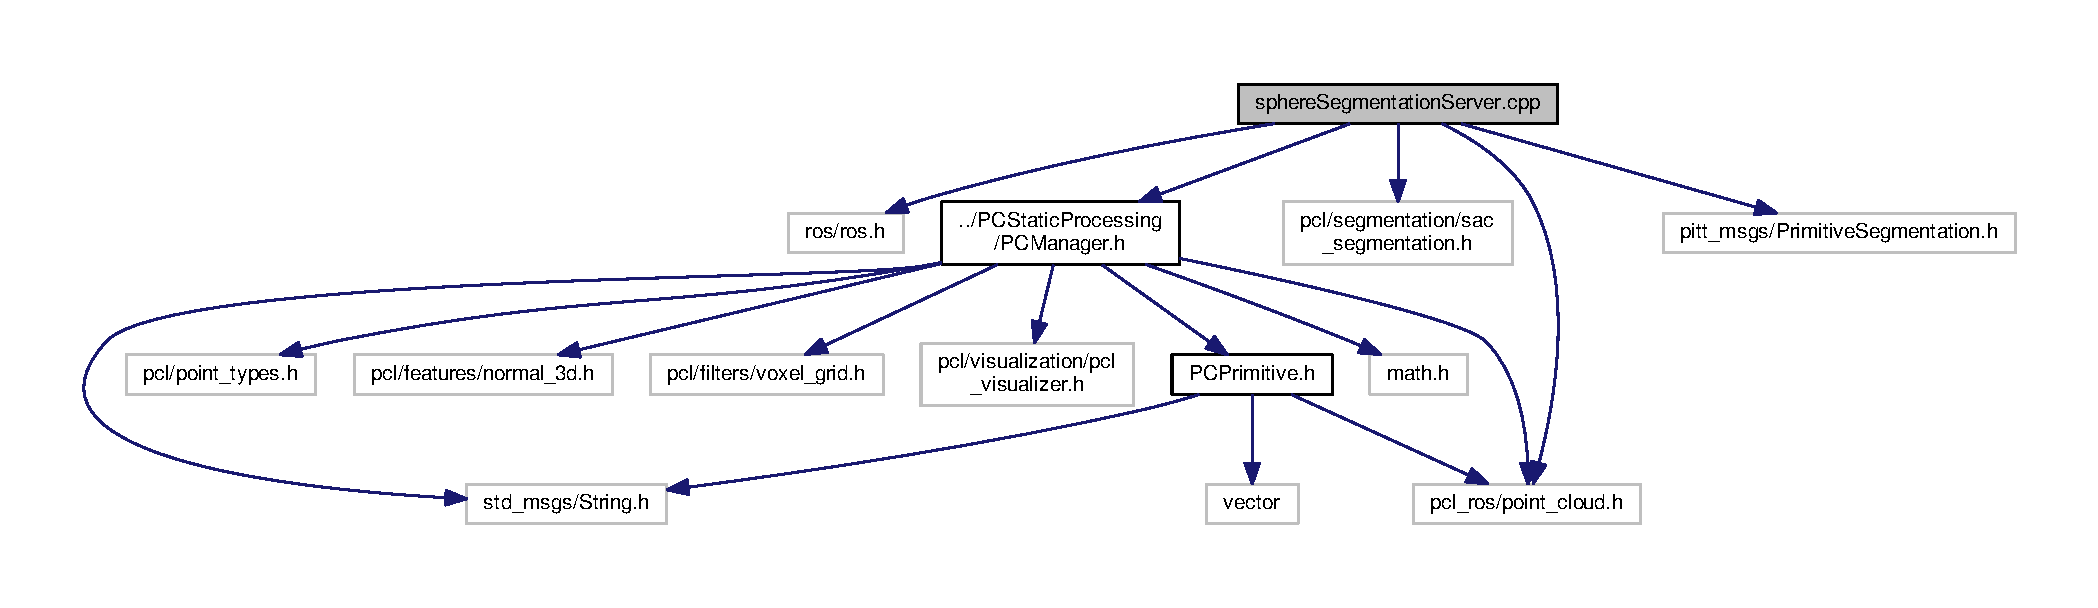
\includegraphics[width=350pt]{sphereSegmentationServer_8cpp__incl}
\end{center}
\end{figure}
\subsection*{Functions}
\begin{DoxyCompactItemize}
\item 
bool \hyperlink{sphereSegmentationServer_8cpp_adc8453905091e0e209797de915728314}{ransac\-Sphere\-Detaction} (Primitive\-Segmentation\-::\-Request \&req, Primitive\-Segmentation\-::\-Response \&res)
\item 
int \hyperlink{sphereSegmentationServer_8cpp_a3c04138a5bfe5d72780bb7e82a18e627}{main} (int argc, char $\ast$$\ast$argv)
\end{DoxyCompactItemize}
\subsection*{Variables}
\begin{DoxyCompactItemize}
\item 
const float \hyperlink{sphereSegmentationServer_8cpp_a6a60b5e5200860d75f403dcf05dde9ef}{N\-O\-R\-M\-A\-L\-\_\-\-D\-I\-S\-T\-A\-N\-C\-E\-\_\-\-W\-E\-I\-G\-H\-T\-\_\-\-D\-E\-F\-A\-U\-L\-T} = 0.\-001f
\item 
const float \hyperlink{sphereSegmentationServer_8cpp_a73e7be3a150e91558f7c5e69c03dd6e6}{D\-I\-S\-T\-A\-N\-C\-E\-\_\-\-T\-H\-R\-E\-S\-H\-O\-L\-D\-\_\-\-D\-E\-F\-A\-U\-L\-T} = 0.\-007f
\item 
const int \hyperlink{sphereSegmentationServer_8cpp_aeb805bfa6116e2c314b0ebc3c73c6504}{M\-A\-X\-\_\-\-I\-T\-E\-R\-A\-T\-I\-O\-N\-\_\-\-D\-E\-F\-A\-U\-L\-T} = 1000
\item 
const float \hyperlink{sphereSegmentationServer_8cpp_aa84d6979d2a503e253f54c3e069abaf5}{M\-I\-N\-\_\-\-R\-A\-D\-I\-U\-S\-\_\-\-L\-I\-M\-I\-T} = 0.\-005
\item 
const float \hyperlink{sphereSegmentationServer_8cpp_abcdbdc04946f1566041df18c6c892f0f}{M\-A\-X\-\_\-\-R\-A\-D\-I\-U\-S\-\_\-\-L\-I\-M\-I\-T} = 0.\-500
\item 
const float \hyperlink{sphereSegmentationServer_8cpp_a32a067fb9ad7cc8e19b52018946d374d}{E\-P\-S\-\_\-\-A\-N\-G\-L\-E} = 0.\-0f
\item 
const float \hyperlink{sphereSegmentationServer_8cpp_ae71c4fb043a78285d76d4dcbd7231e70}{M\-I\-N\-\_\-\-O\-P\-E\-N\-I\-N\-G\-\_\-\-A\-N\-G\-L\-E} = 100.\-0f
\item 
const float \hyperlink{sphereSegmentationServer_8cpp_afaeeefd6f578a58f8e14040f6176c394}{M\-A\-X\-\_\-\-O\-P\-E\-N\-I\-N\-G\-\_\-\-A\-N\-G\-L\-E} = 180.\-0f
\end{DoxyCompactItemize}


\subsection{Function Documentation}
\hypertarget{sphereSegmentationServer_8cpp_a3c04138a5bfe5d72780bb7e82a18e627}{\index{sphere\-Segmentation\-Server.\-cpp@{sphere\-Segmentation\-Server.\-cpp}!main@{main}}
\index{main@{main}!sphereSegmentationServer.cpp@{sphere\-Segmentation\-Server.\-cpp}}
\subsubsection[{main}]{\setlength{\rightskip}{0pt plus 5cm}int main (
\begin{DoxyParamCaption}
\item[{int}]{argc, }
\item[{char $\ast$$\ast$}]{argv}
\end{DoxyParamCaption}
)}}\label{sphereSegmentationServer_8cpp_a3c04138a5bfe5d72780bb7e82a18e627}


Definition at line 113 of file sphere\-Segmentation\-Server.\-cpp.



References pcm\-::\-P\-C\-Manager\-::\-R\-A\-N\-S\-A\-C\-\_\-\-S\-P\-H\-E\-R\-E\-\_\-\-F\-I\-L\-T\-E\-R\-\_\-\-S\-E\-R\-V\-I\-C\-E\-\_\-\-N\-A\-M\-E, and ransac\-Sphere\-Detaction().



Here is the call graph for this function\-:\nopagebreak
\begin{figure}[H]
\begin{center}
\leavevmode
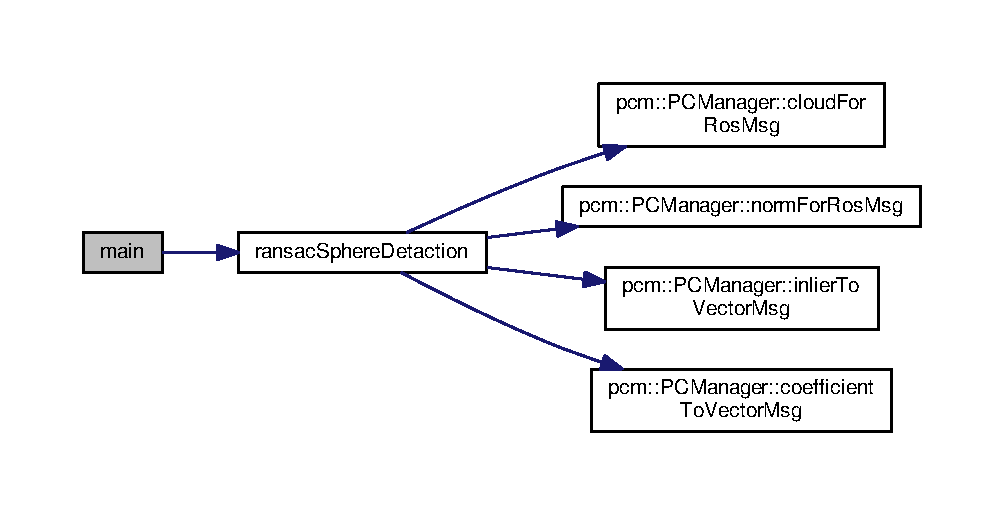
\includegraphics[width=350pt]{sphereSegmentationServer_8cpp_a3c04138a5bfe5d72780bb7e82a18e627_cgraph}
\end{center}
\end{figure}


\hypertarget{sphereSegmentationServer_8cpp_adc8453905091e0e209797de915728314}{\index{sphere\-Segmentation\-Server.\-cpp@{sphere\-Segmentation\-Server.\-cpp}!ransac\-Sphere\-Detaction@{ransac\-Sphere\-Detaction}}
\index{ransac\-Sphere\-Detaction@{ransac\-Sphere\-Detaction}!sphereSegmentationServer.cpp@{sphere\-Segmentation\-Server.\-cpp}}
\subsubsection[{ransac\-Sphere\-Detaction}]{\setlength{\rightskip}{0pt plus 5cm}bool ransac\-Sphere\-Detaction (
\begin{DoxyParamCaption}
\item[{Primitive\-Segmentation\-::\-Request \&}]{req, }
\item[{Primitive\-Segmentation\-::\-Response \&}]{res}
\end{DoxyParamCaption}
)}}\label{sphereSegmentationServer_8cpp_adc8453905091e0e209797de915728314}


Definition at line 26 of file sphere\-Segmentation\-Server.\-cpp.



References pcm\-::\-P\-C\-Manager\-::cloud\-For\-Ros\-Msg(), pcm\-::\-P\-C\-Manager\-::coefficient\-To\-Vector\-Msg(), D\-I\-S\-T\-A\-N\-C\-E\-\_\-\-T\-H\-R\-E\-S\-H\-O\-L\-D\-\_\-\-D\-E\-F\-A\-U\-L\-T, E\-P\-S\-\_\-\-A\-N\-G\-L\-E, pcm\-::\-P\-C\-Manager\-::inlier\-To\-Vector\-Msg(), M\-A\-X\-\_\-\-I\-T\-E\-R\-A\-T\-I\-O\-N\-\_\-\-D\-E\-F\-A\-U\-L\-T, M\-A\-X\-\_\-\-O\-P\-E\-N\-I\-N\-G\-\_\-\-A\-N\-G\-L\-E, M\-A\-X\-\_\-\-R\-A\-D\-I\-U\-S\-\_\-\-L\-I\-M\-I\-T, M\-I\-N\-\_\-\-O\-P\-E\-N\-I\-N\-G\-\_\-\-A\-N\-G\-L\-E, M\-I\-N\-\_\-\-R\-A\-D\-I\-U\-S\-\_\-\-L\-I\-M\-I\-T, N\-O\-R\-M\-A\-L\-\_\-\-D\-I\-S\-T\-A\-N\-C\-E\-\_\-\-W\-E\-I\-G\-H\-T\-\_\-\-D\-E\-F\-A\-U\-L\-T, pcm\-::\-P\-C\-Manager\-::norm\-For\-Ros\-Msg(), and seg.



Referenced by main().



Here is the call graph for this function\-:\nopagebreak
\begin{figure}[H]
\begin{center}
\leavevmode
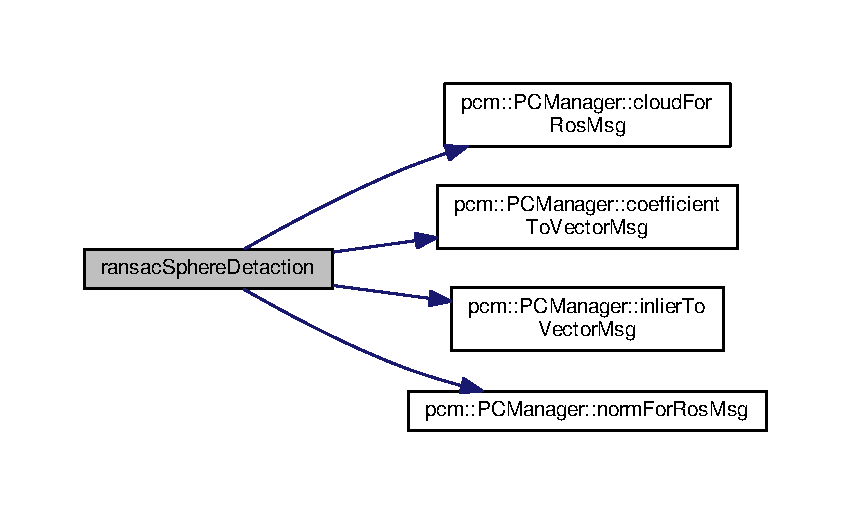
\includegraphics[width=350pt]{sphereSegmentationServer_8cpp_adc8453905091e0e209797de915728314_cgraph}
\end{center}
\end{figure}




\subsection{Variable Documentation}
\hypertarget{sphereSegmentationServer_8cpp_a73e7be3a150e91558f7c5e69c03dd6e6}{\index{sphere\-Segmentation\-Server.\-cpp@{sphere\-Segmentation\-Server.\-cpp}!D\-I\-S\-T\-A\-N\-C\-E\-\_\-\-T\-H\-R\-E\-S\-H\-O\-L\-D\-\_\-\-D\-E\-F\-A\-U\-L\-T@{D\-I\-S\-T\-A\-N\-C\-E\-\_\-\-T\-H\-R\-E\-S\-H\-O\-L\-D\-\_\-\-D\-E\-F\-A\-U\-L\-T}}
\index{D\-I\-S\-T\-A\-N\-C\-E\-\_\-\-T\-H\-R\-E\-S\-H\-O\-L\-D\-\_\-\-D\-E\-F\-A\-U\-L\-T@{D\-I\-S\-T\-A\-N\-C\-E\-\_\-\-T\-H\-R\-E\-S\-H\-O\-L\-D\-\_\-\-D\-E\-F\-A\-U\-L\-T}!sphereSegmentationServer.cpp@{sphere\-Segmentation\-Server.\-cpp}}
\subsubsection[{D\-I\-S\-T\-A\-N\-C\-E\-\_\-\-T\-H\-R\-E\-S\-H\-O\-L\-D\-\_\-\-D\-E\-F\-A\-U\-L\-T}]{\setlength{\rightskip}{0pt plus 5cm}const float D\-I\-S\-T\-A\-N\-C\-E\-\_\-\-T\-H\-R\-E\-S\-H\-O\-L\-D\-\_\-\-D\-E\-F\-A\-U\-L\-T = 0.\-007f}}\label{sphereSegmentationServer_8cpp_a73e7be3a150e91558f7c5e69c03dd6e6}


Definition at line 17 of file sphere\-Segmentation\-Server.\-cpp.



Referenced by ransac\-Sphere\-Detaction().

\hypertarget{sphereSegmentationServer_8cpp_a32a067fb9ad7cc8e19b52018946d374d}{\index{sphere\-Segmentation\-Server.\-cpp@{sphere\-Segmentation\-Server.\-cpp}!E\-P\-S\-\_\-\-A\-N\-G\-L\-E@{E\-P\-S\-\_\-\-A\-N\-G\-L\-E}}
\index{E\-P\-S\-\_\-\-A\-N\-G\-L\-E@{E\-P\-S\-\_\-\-A\-N\-G\-L\-E}!sphereSegmentationServer.cpp@{sphere\-Segmentation\-Server.\-cpp}}
\subsubsection[{E\-P\-S\-\_\-\-A\-N\-G\-L\-E}]{\setlength{\rightskip}{0pt plus 5cm}const float E\-P\-S\-\_\-\-A\-N\-G\-L\-E = 0.\-0f}}\label{sphereSegmentationServer_8cpp_a32a067fb9ad7cc8e19b52018946d374d}


Definition at line 21 of file sphere\-Segmentation\-Server.\-cpp.



Referenced by ransac\-Sphere\-Detaction().

\hypertarget{sphereSegmentationServer_8cpp_aeb805bfa6116e2c314b0ebc3c73c6504}{\index{sphere\-Segmentation\-Server.\-cpp@{sphere\-Segmentation\-Server.\-cpp}!M\-A\-X\-\_\-\-I\-T\-E\-R\-A\-T\-I\-O\-N\-\_\-\-D\-E\-F\-A\-U\-L\-T@{M\-A\-X\-\_\-\-I\-T\-E\-R\-A\-T\-I\-O\-N\-\_\-\-D\-E\-F\-A\-U\-L\-T}}
\index{M\-A\-X\-\_\-\-I\-T\-E\-R\-A\-T\-I\-O\-N\-\_\-\-D\-E\-F\-A\-U\-L\-T@{M\-A\-X\-\_\-\-I\-T\-E\-R\-A\-T\-I\-O\-N\-\_\-\-D\-E\-F\-A\-U\-L\-T}!sphereSegmentationServer.cpp@{sphere\-Segmentation\-Server.\-cpp}}
\subsubsection[{M\-A\-X\-\_\-\-I\-T\-E\-R\-A\-T\-I\-O\-N\-\_\-\-D\-E\-F\-A\-U\-L\-T}]{\setlength{\rightskip}{0pt plus 5cm}const int M\-A\-X\-\_\-\-I\-T\-E\-R\-A\-T\-I\-O\-N\-\_\-\-D\-E\-F\-A\-U\-L\-T = 1000}}\label{sphereSegmentationServer_8cpp_aeb805bfa6116e2c314b0ebc3c73c6504}


Definition at line 18 of file sphere\-Segmentation\-Server.\-cpp.



Referenced by ransac\-Sphere\-Detaction().

\hypertarget{sphereSegmentationServer_8cpp_afaeeefd6f578a58f8e14040f6176c394}{\index{sphere\-Segmentation\-Server.\-cpp@{sphere\-Segmentation\-Server.\-cpp}!M\-A\-X\-\_\-\-O\-P\-E\-N\-I\-N\-G\-\_\-\-A\-N\-G\-L\-E@{M\-A\-X\-\_\-\-O\-P\-E\-N\-I\-N\-G\-\_\-\-A\-N\-G\-L\-E}}
\index{M\-A\-X\-\_\-\-O\-P\-E\-N\-I\-N\-G\-\_\-\-A\-N\-G\-L\-E@{M\-A\-X\-\_\-\-O\-P\-E\-N\-I\-N\-G\-\_\-\-A\-N\-G\-L\-E}!sphereSegmentationServer.cpp@{sphere\-Segmentation\-Server.\-cpp}}
\subsubsection[{M\-A\-X\-\_\-\-O\-P\-E\-N\-I\-N\-G\-\_\-\-A\-N\-G\-L\-E}]{\setlength{\rightskip}{0pt plus 5cm}const float M\-A\-X\-\_\-\-O\-P\-E\-N\-I\-N\-G\-\_\-\-A\-N\-G\-L\-E = 180.\-0f}}\label{sphereSegmentationServer_8cpp_afaeeefd6f578a58f8e14040f6176c394}


Definition at line 23 of file sphere\-Segmentation\-Server.\-cpp.



Referenced by ransac\-Sphere\-Detaction().

\hypertarget{sphereSegmentationServer_8cpp_abcdbdc04946f1566041df18c6c892f0f}{\index{sphere\-Segmentation\-Server.\-cpp@{sphere\-Segmentation\-Server.\-cpp}!M\-A\-X\-\_\-\-R\-A\-D\-I\-U\-S\-\_\-\-L\-I\-M\-I\-T@{M\-A\-X\-\_\-\-R\-A\-D\-I\-U\-S\-\_\-\-L\-I\-M\-I\-T}}
\index{M\-A\-X\-\_\-\-R\-A\-D\-I\-U\-S\-\_\-\-L\-I\-M\-I\-T@{M\-A\-X\-\_\-\-R\-A\-D\-I\-U\-S\-\_\-\-L\-I\-M\-I\-T}!sphereSegmentationServer.cpp@{sphere\-Segmentation\-Server.\-cpp}}
\subsubsection[{M\-A\-X\-\_\-\-R\-A\-D\-I\-U\-S\-\_\-\-L\-I\-M\-I\-T}]{\setlength{\rightskip}{0pt plus 5cm}const float M\-A\-X\-\_\-\-R\-A\-D\-I\-U\-S\-\_\-\-L\-I\-M\-I\-T = 0.\-500}}\label{sphereSegmentationServer_8cpp_abcdbdc04946f1566041df18c6c892f0f}


Definition at line 20 of file sphere\-Segmentation\-Server.\-cpp.



Referenced by ransac\-Sphere\-Detaction().

\hypertarget{sphereSegmentationServer_8cpp_ae71c4fb043a78285d76d4dcbd7231e70}{\index{sphere\-Segmentation\-Server.\-cpp@{sphere\-Segmentation\-Server.\-cpp}!M\-I\-N\-\_\-\-O\-P\-E\-N\-I\-N\-G\-\_\-\-A\-N\-G\-L\-E@{M\-I\-N\-\_\-\-O\-P\-E\-N\-I\-N\-G\-\_\-\-A\-N\-G\-L\-E}}
\index{M\-I\-N\-\_\-\-O\-P\-E\-N\-I\-N\-G\-\_\-\-A\-N\-G\-L\-E@{M\-I\-N\-\_\-\-O\-P\-E\-N\-I\-N\-G\-\_\-\-A\-N\-G\-L\-E}!sphereSegmentationServer.cpp@{sphere\-Segmentation\-Server.\-cpp}}
\subsubsection[{M\-I\-N\-\_\-\-O\-P\-E\-N\-I\-N\-G\-\_\-\-A\-N\-G\-L\-E}]{\setlength{\rightskip}{0pt plus 5cm}const float M\-I\-N\-\_\-\-O\-P\-E\-N\-I\-N\-G\-\_\-\-A\-N\-G\-L\-E = 100.\-0f}}\label{sphereSegmentationServer_8cpp_ae71c4fb043a78285d76d4dcbd7231e70}


Definition at line 22 of file sphere\-Segmentation\-Server.\-cpp.



Referenced by ransac\-Sphere\-Detaction().

\hypertarget{sphereSegmentationServer_8cpp_aa84d6979d2a503e253f54c3e069abaf5}{\index{sphere\-Segmentation\-Server.\-cpp@{sphere\-Segmentation\-Server.\-cpp}!M\-I\-N\-\_\-\-R\-A\-D\-I\-U\-S\-\_\-\-L\-I\-M\-I\-T@{M\-I\-N\-\_\-\-R\-A\-D\-I\-U\-S\-\_\-\-L\-I\-M\-I\-T}}
\index{M\-I\-N\-\_\-\-R\-A\-D\-I\-U\-S\-\_\-\-L\-I\-M\-I\-T@{M\-I\-N\-\_\-\-R\-A\-D\-I\-U\-S\-\_\-\-L\-I\-M\-I\-T}!sphereSegmentationServer.cpp@{sphere\-Segmentation\-Server.\-cpp}}
\subsubsection[{M\-I\-N\-\_\-\-R\-A\-D\-I\-U\-S\-\_\-\-L\-I\-M\-I\-T}]{\setlength{\rightskip}{0pt plus 5cm}const float M\-I\-N\-\_\-\-R\-A\-D\-I\-U\-S\-\_\-\-L\-I\-M\-I\-T = 0.\-005}}\label{sphereSegmentationServer_8cpp_aa84d6979d2a503e253f54c3e069abaf5}


Definition at line 19 of file sphere\-Segmentation\-Server.\-cpp.



Referenced by ransac\-Sphere\-Detaction().

\hypertarget{sphereSegmentationServer_8cpp_a6a60b5e5200860d75f403dcf05dde9ef}{\index{sphere\-Segmentation\-Server.\-cpp@{sphere\-Segmentation\-Server.\-cpp}!N\-O\-R\-M\-A\-L\-\_\-\-D\-I\-S\-T\-A\-N\-C\-E\-\_\-\-W\-E\-I\-G\-H\-T\-\_\-\-D\-E\-F\-A\-U\-L\-T@{N\-O\-R\-M\-A\-L\-\_\-\-D\-I\-S\-T\-A\-N\-C\-E\-\_\-\-W\-E\-I\-G\-H\-T\-\_\-\-D\-E\-F\-A\-U\-L\-T}}
\index{N\-O\-R\-M\-A\-L\-\_\-\-D\-I\-S\-T\-A\-N\-C\-E\-\_\-\-W\-E\-I\-G\-H\-T\-\_\-\-D\-E\-F\-A\-U\-L\-T@{N\-O\-R\-M\-A\-L\-\_\-\-D\-I\-S\-T\-A\-N\-C\-E\-\_\-\-W\-E\-I\-G\-H\-T\-\_\-\-D\-E\-F\-A\-U\-L\-T}!sphereSegmentationServer.cpp@{sphere\-Segmentation\-Server.\-cpp}}
\subsubsection[{N\-O\-R\-M\-A\-L\-\_\-\-D\-I\-S\-T\-A\-N\-C\-E\-\_\-\-W\-E\-I\-G\-H\-T\-\_\-\-D\-E\-F\-A\-U\-L\-T}]{\setlength{\rightskip}{0pt plus 5cm}const float N\-O\-R\-M\-A\-L\-\_\-\-D\-I\-S\-T\-A\-N\-C\-E\-\_\-\-W\-E\-I\-G\-H\-T\-\_\-\-D\-E\-F\-A\-U\-L\-T = 0.\-001f}}\label{sphereSegmentationServer_8cpp_a6a60b5e5200860d75f403dcf05dde9ef}


Definition at line 16 of file sphere\-Segmentation\-Server.\-cpp.



Referenced by ransac\-Sphere\-Detaction().


\hypertarget{supportsSegmentationServer_8cpp}{\section{supports\-Segmentation\-Server.\-cpp File Reference}
\label{supportsSegmentationServer_8cpp}\index{supports\-Segmentation\-Server.\-cpp@{supports\-Segmentation\-Server.\-cpp}}
}
{\ttfamily \#include \char`\"{}ros/ros.\-h\char`\"{}}\\*
{\ttfamily \#include $<$iostream$>$}\\*
{\ttfamily \#include \char`\"{}math.\-h\char`\"{}}\\*
{\ttfamily \#include $<$pcl\-\_\-ros/point\-\_\-cloud.\-h$>$}\\*
{\ttfamily \#include $<$std\-\_\-msgs/\-String.\-h$>$}\\*
{\ttfamily \#include $<$pcl/segmentation/sac\-\_\-segmentation.\-h$>$}\\*
{\ttfamily \#include $<$pcl/filters/extract\-\_\-indices.\-h$>$}\\*
{\ttfamily \#include \char`\"{}pitt\-\_\-msgs/\-Support\-Segmentation.\-h\char`\"{}}\\*
{\ttfamily \#include \char`\"{}pitt\-\_\-msgs/\-Inliers\-Support.\-h\char`\"{}}\\*
{\ttfamily \#include \char`\"{}../\-P\-C\-Static\-Processing/\-P\-C\-Manager.\-h\char`\"{}}\\*
Include dependency graph for supports\-Segmentation\-Server.\-cpp\-:\nopagebreak
\begin{figure}[H]
\begin{center}
\leavevmode
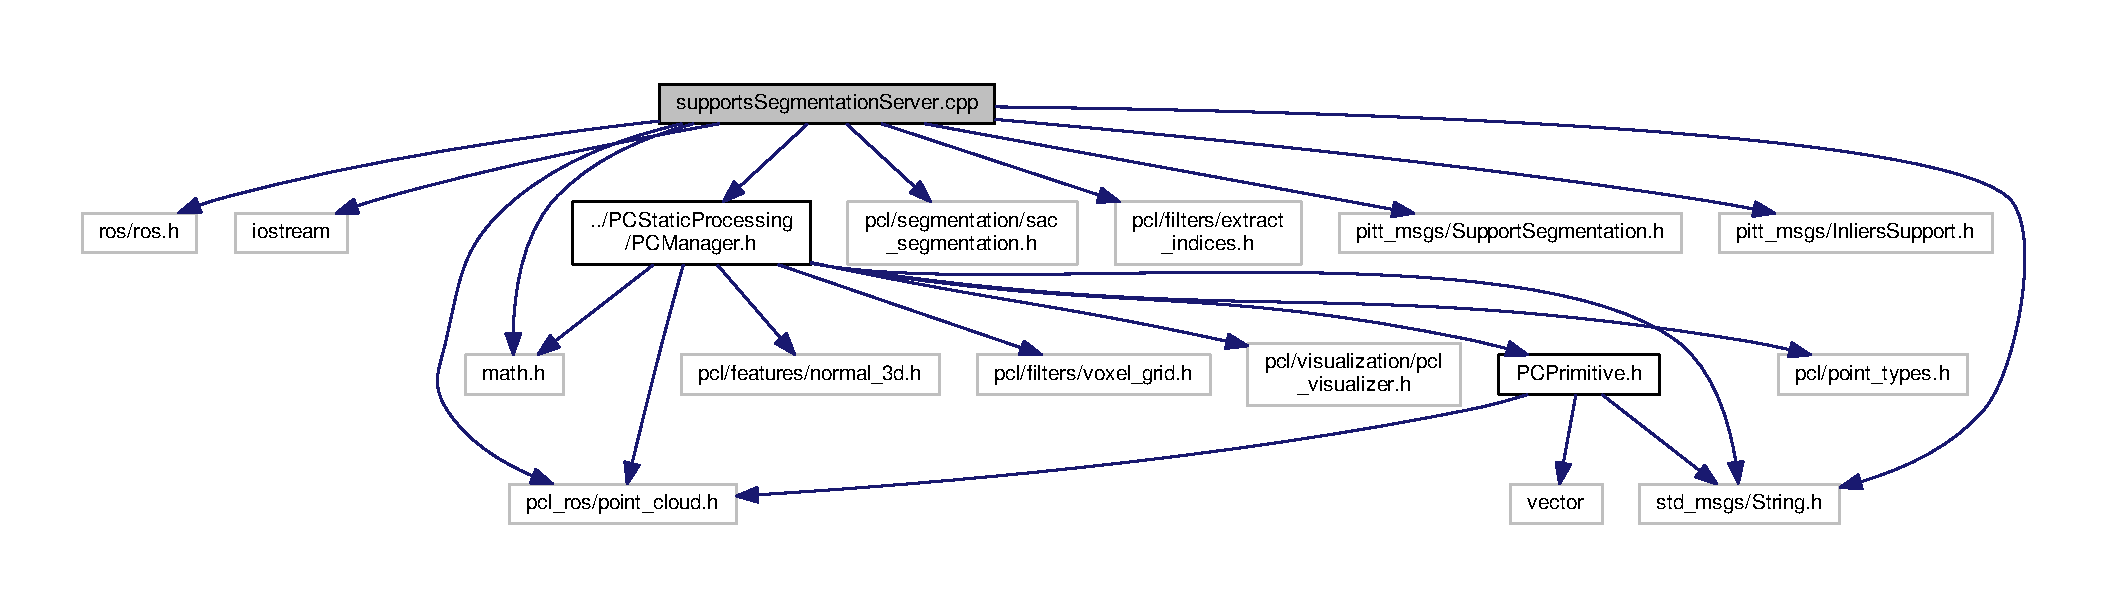
\includegraphics[width=350pt]{supportsSegmentationServer_8cpp__incl}
\end{center}
\end{figure}
\subsection*{Macros}
\begin{DoxyCompactItemize}
\item 
\#define \hyperlink{supportsSegmentationServer_8cpp_a036699b594fc2e37ecd35243a0a7e2bb}{L\-E\-S\-S\-\_\-\-I\-N\-F}~-\/9999999.\-0
\item 
\#define \hyperlink{supportsSegmentationServer_8cpp_a12c2040f25d8e3a7b9e1c2024c618cb6}{I\-N\-F}~9999999.\-0
\end{DoxyCompactItemize}
\subsection*{Functions}
\begin{DoxyCompactItemize}
\item 
void \hyperlink{supportsSegmentationServer_8cpp_a53687def603ff613a673c0dd550acf4e}{initialize\-Parameters} (Support\-Segmentation\-::\-Request \&req)
\item 
void \hyperlink{supportsSegmentationServer_8cpp_a93fe6461918fe6c40665c81167c39f43}{ransac\-Plane\-Segmentator} (\hyperlink{PCPrimitive_8h_aa14a240c8d999c4f56133c0f70e88783}{P\-C\-L\-Cloud\-Ptr} input\-Cloud, \hyperlink{PCPrimitive_8h_a1bc38ce8b0c26e5f2d28fae9f3e3ea97}{P\-C\-L\-Normal\-Ptr} normals, Point\-Indices\-::\-Ptr \&inlier\-Output, Model\-Coefficients\-::\-Ptr \&coefficient\-Output)
\item 
Extract\-Indices$<$ Point\-X\-Y\-Z $>$ \hyperlink{supportsSegmentationServer_8cpp_ad788fb6fb1f61d45a10993e909fddad8}{extract} (true)
\item 
void \hyperlink{supportsSegmentationServer_8cpp_aec3cb01834351aa77d85fb42364ff543}{remove\-Plane\-Inliner} (\hyperlink{PCPrimitive_8h_aa14a240c8d999c4f56133c0f70e88783}{P\-C\-L\-Cloud\-Ptr} input\-Cloud, Point\-Indices\-::\-Ptr \&remove\-Index, \hyperlink{PCPrimitive_8h_aa14a240c8d999c4f56133c0f70e88783}{P\-C\-L\-Cloud\-Ptr} output)
\item 
bool \hyperlink{supportsSegmentationServer_8cpp_af7452b4e42ac3352d3b9ff7c19dff6ea}{value\-Belongs\-To\-Array} (int value, Point\-Indices\-::\-Ptr inliers)
\item 
\hyperlink{PCPrimitive_8h_a6ec0f6fbb026ae4b66cac121673c3a8a}{Primitive\-Idx\-Ptr} \hyperlink{supportsSegmentationServer_8cpp_a32c40c5b97dadeee297fd5e4f8d36513}{create\-New\-Idx\-Map} (\hyperlink{PCPrimitive_8h_a6ec0f6fbb026ae4b66cac121673c3a8a}{Primitive\-Idx\-Ptr} previous\-Inliers\-Map, Point\-Indices\-::\-Ptr inliers, int level)
\item 
bool \hyperlink{supportsSegmentationServer_8cpp_ab0fa44eb10c2965d2e3a67a7f386c747}{is\-Horizontal\-Plane} (\hyperlink{PCPrimitive_8h_a1bc38ce8b0c26e5f2d28fae9f3e3ea97}{P\-C\-L\-Normal\-Ptr} normal, Model\-Coefficients\-::\-Ptr coefficients, const float referiment\-Axis\mbox{[}3\mbox{]})
\item 
\hyperlink{PCPrimitive_8h_aa14a240c8d999c4f56133c0f70e88783}{P\-C\-L\-Cloud\-Ptr} \hyperlink{supportsSegmentationServer_8cpp_a7788e49ce18c43d68c6e9b31f7c8c1eb}{get\-Point\-On\-Plane} (\hyperlink{PCPrimitive_8h_aa14a240c8d999c4f56133c0f70e88783}{P\-C\-L\-Cloud\-Ptr} plane, \hyperlink{PCPrimitive_8h_a6ec0f6fbb026ae4b66cac121673c3a8a}{Primitive\-Idx\-Ptr} inlier\-Idx, int map\-Level)
\item 
bool \hyperlink{supportsSegmentationServer_8cpp_a5516ae3363218ea9eafda7f65e6d2a49}{find\-Supports} (Support\-Segmentation\-::\-Request \&req, Support\-Segmentation\-::\-Response \&res)
\item 
int \hyperlink{supportsSegmentationServer_8cpp_a3c04138a5bfe5d72780bb7e82a18e627}{main} (int argc, char $\ast$$\ast$argv)
\end{DoxyCompactItemize}
\subsection*{Variables}
\begin{DoxyCompactItemize}
\item 
static const float \hyperlink{supportsSegmentationServer_8cpp_af8b66843d91c073a7339d97da05e4cfa}{M\-I\-N\-\_\-\-I\-T\-E\-R\-A\-T\-I\-V\-E\-\_\-\-C\-L\-O\-U\-D\-\_\-\-P\-E\-R\-C\-E\-N\-T\-U\-A\-L\-\_\-\-S\-I\-Z\-E} = 0.\-030f
\item 
static const float \hyperlink{supportsSegmentationServer_8cpp_a1cb5f58d4341fb0ea8be5786e76e850c}{M\-I\-N\-\_\-\-P\-L\-A\-N\-E\-\_\-\-P\-E\-R\-C\-E\-N\-T\-A\-G\-E\-\_\-\-S\-I\-Z\-E} = 0.\-030f
\item 
static const float \hyperlink{supportsSegmentationServer_8cpp_a31976c93f57ecffe05dcdb46e5a1eb4a}{M\-A\-X\-\_\-\-V\-A\-R\-I\-A\-N\-C\-E\-\_\-\-T\-H\-\_\-\-F\-O\-R\-\_\-\-H\-O\-R\-I\-Z\-O\-N\-T\-A\-L} = 0.\-09f
\item 
static const int \hyperlink{supportsSegmentationServer_8cpp_acc65cc4496947189ecf64074b20c9a6b}{R\-A\-N\-S\-A\-C\-\_\-\-M\-A\-X\-\_\-\-I\-T\-E\-R\-A\-T\-I\-O\-N\-\_\-\-T\-H} = 10
\item 
static const float \hyperlink{supportsSegmentationServer_8cpp_ab8a45d894e93cb97afbd56586a97172d}{R\-A\-N\-S\-A\-C\-\_\-\-T\-H\-\_\-\-D\-I\-S\-T\-A\-N\-C\-E\-\_\-\-P\-O\-I\-N\-T\-\_\-\-S\-H\-A\-P\-E} = 0.\-02f
\item 
static const float \hyperlink{supportsSegmentationServer_8cpp_a9dc99e81f4ba41b83214b0d6b629dd10}{R\-A\-N\-S\-A\-C\-\_\-\-N\-O\-R\-M\-A\-L\-\_\-\-D\-I\-S\-T\-A\-N\-C\-E\-\_\-\-W\-E\-I\-G\-H\-T} = 0.\-9f
\item 
static const float \hyperlink{supportsSegmentationServer_8cpp_a7e5e89000afcc1ee5b2f3aca14c819d8}{H\-O\-R\-I\-Z\-O\-N\-T\-A\-L\-\_\-\-A\-X\-I\-S} \mbox{[}3\mbox{]} = \{ 0.\-0f, 0.\-0f, -\/1.\-0f\}
\item 
static const float \hyperlink{supportsSegmentationServer_8cpp_a7ea400b8bac873942021139dabfda6be}{S\-U\-P\-P\-O\-R\-T\-\_\-\-E\-D\-G\-\_\-\-R\-E\-M\-O\-V\-E\-E\-\_\-\-O\-F\-S\-E\-T} = 0.\-02
\item 
float \hyperlink{supportsSegmentationServer_8cpp_aad09e65ed4fbd692157ce317f949c892}{min\-Iterative\-Cloud\-Percentage}
\item 
float \hyperlink{supportsSegmentationServer_8cpp_a4347491f1f8b99276368828ab1133658}{min\-Plane\-Percentage\-Size}
\item 
float \hyperlink{supportsSegmentationServer_8cpp_a197bb458bd6fcbde04f684821eec83fb}{min\-Variance\-Th\-For\-Horizontal}
\item 
float \hyperlink{supportsSegmentationServer_8cpp_af902851fe5d5f9b83a6fd3caa09ff6e6}{max\-Variance\-Th\-For\-Horizontal}
\item 
float \hyperlink{supportsSegmentationServer_8cpp_acb13e2ccfe978df3c0ae59f3209561e7}{ransac\-Th\-Distance\-Point\-Shape}
\item 
float \hyperlink{supportsSegmentationServer_8cpp_ad870cd7d7c56cf82343d1a2a59072627}{ransac\-Normale\-Distance\-Weigth}
\item 
float \hyperlink{supportsSegmentationServer_8cpp_a99daf6bf3b99a58055b66c72a8040bef}{support\-Edge\-Remove\-Ofset}
\item 
float \hyperlink{supportsSegmentationServer_8cpp_aba5cf30daaf1f4bd0b577e2a1eaacc1f}{horizontal\-Axis} \mbox{[}3\mbox{]}
\item 
int \hyperlink{supportsSegmentationServer_8cpp_adf23ae5b5b90ea992496e126ae78a3a5}{ransac\-Max\-Iteration}
\item 
\hyperlink{PCManager_8h_a38c805dbc7ad6f06109b85c8e540817a}{P\-C\-L\-Visualizer} \hyperlink{supportsSegmentationServer_8cpp_abb8f65165b6cd9a52d46c3f8dab2872f}{vis}
\item 
\hyperlink{PCPrimitive_8h_aa14a240c8d999c4f56133c0f70e88783}{P\-C\-L\-Cloud\-Ptr} \hyperlink{supportsSegmentationServer_8cpp_ac8a873b38ae54d8231e11fc61c6abc54}{original\-Cloud}
\item 
\hyperlink{PCPrimitive_8h_a1bc38ce8b0c26e5f2d28fae9f3e3ea97}{P\-C\-L\-Normal\-Ptr} \hyperlink{supportsSegmentationServer_8cpp_a2974d140b39b60770786decb2d3565b1}{original\-Norms}
\item 
S\-A\-C\-Segmentation\-From\-Normals\\*
$<$ Point\-X\-Y\-Z, Normal $>$ \hyperlink{supportsSegmentationServer_8cpp_ac380aeac6f81ac15dbab87458f1309f1}{seg}
\end{DoxyCompactItemize}


\subsection{Macro Definition Documentation}
\hypertarget{supportsSegmentationServer_8cpp_a12c2040f25d8e3a7b9e1c2024c618cb6}{\index{supports\-Segmentation\-Server.\-cpp@{supports\-Segmentation\-Server.\-cpp}!I\-N\-F@{I\-N\-F}}
\index{I\-N\-F@{I\-N\-F}!supportsSegmentationServer.cpp@{supports\-Segmentation\-Server.\-cpp}}
\subsubsection[{I\-N\-F}]{\setlength{\rightskip}{0pt plus 5cm}\#define I\-N\-F~9999999.\-0}}\label{supportsSegmentationServer_8cpp_a12c2040f25d8e3a7b9e1c2024c618cb6}


Definition at line 188 of file supports\-Segmentation\-Server.\-cpp.



Referenced by get\-Point\-On\-Plane().

\hypertarget{supportsSegmentationServer_8cpp_a036699b594fc2e37ecd35243a0a7e2bb}{\index{supports\-Segmentation\-Server.\-cpp@{supports\-Segmentation\-Server.\-cpp}!L\-E\-S\-S\-\_\-\-I\-N\-F@{L\-E\-S\-S\-\_\-\-I\-N\-F}}
\index{L\-E\-S\-S\-\_\-\-I\-N\-F@{L\-E\-S\-S\-\_\-\-I\-N\-F}!supportsSegmentationServer.cpp@{supports\-Segmentation\-Server.\-cpp}}
\subsubsection[{L\-E\-S\-S\-\_\-\-I\-N\-F}]{\setlength{\rightskip}{0pt plus 5cm}\#define L\-E\-S\-S\-\_\-\-I\-N\-F~-\/9999999.\-0}}\label{supportsSegmentationServer_8cpp_a036699b594fc2e37ecd35243a0a7e2bb}


Definition at line 187 of file supports\-Segmentation\-Server.\-cpp.



Referenced by get\-Point\-On\-Plane().



\subsection{Function Documentation}
\hypertarget{supportsSegmentationServer_8cpp_a32c40c5b97dadeee297fd5e4f8d36513}{\index{supports\-Segmentation\-Server.\-cpp@{supports\-Segmentation\-Server.\-cpp}!create\-New\-Idx\-Map@{create\-New\-Idx\-Map}}
\index{create\-New\-Idx\-Map@{create\-New\-Idx\-Map}!supportsSegmentationServer.cpp@{supports\-Segmentation\-Server.\-cpp}}
\subsubsection[{create\-New\-Idx\-Map}]{\setlength{\rightskip}{0pt plus 5cm}{\bf Primitive\-Idx\-Ptr} create\-New\-Idx\-Map (
\begin{DoxyParamCaption}
\item[{{\bf Primitive\-Idx\-Ptr}}]{previous\-Inliers\-Map, }
\item[{Point\-Indices\-::\-Ptr}]{inliers, }
\item[{int}]{level}
\end{DoxyParamCaption}
)}}\label{supportsSegmentationServer_8cpp_a32c40c5b97dadeee297fd5e4f8d36513}


Definition at line 144 of file supports\-Segmentation\-Server.\-cpp.



References value\-Belongs\-To\-Array().



Referenced by find\-Supports().



Here is the call graph for this function\-:\nopagebreak
\begin{figure}[H]
\begin{center}
\leavevmode
\includegraphics[width=322pt]{supportsSegmentationServer_8cpp_a32c40c5b97dadeee297fd5e4f8d36513_cgraph}
\end{center}
\end{figure}


\hypertarget{supportsSegmentationServer_8cpp_ad788fb6fb1f61d45a10993e909fddad8}{\index{supports\-Segmentation\-Server.\-cpp@{supports\-Segmentation\-Server.\-cpp}!extract@{extract}}
\index{extract@{extract}!supportsSegmentationServer.cpp@{supports\-Segmentation\-Server.\-cpp}}
\subsubsection[{extract}]{\setlength{\rightskip}{0pt plus 5cm}Extract\-Indices$<$ Point\-X\-Y\-Z$>$ extract (
\begin{DoxyParamCaption}
\item[{true}]{}
\end{DoxyParamCaption}
)}}\label{supportsSegmentationServer_8cpp_ad788fb6fb1f61d45a10993e909fddad8}


Referenced by remove\-Plane\-Inliner().

\hypertarget{supportsSegmentationServer_8cpp_a5516ae3363218ea9eafda7f65e6d2a49}{\index{supports\-Segmentation\-Server.\-cpp@{supports\-Segmentation\-Server.\-cpp}!find\-Supports@{find\-Supports}}
\index{find\-Supports@{find\-Supports}!supportsSegmentationServer.cpp@{supports\-Segmentation\-Server.\-cpp}}
\subsubsection[{find\-Supports}]{\setlength{\rightskip}{0pt plus 5cm}bool find\-Supports (
\begin{DoxyParamCaption}
\item[{Support\-Segmentation\-::\-Request \&}]{req, }
\item[{Support\-Segmentation\-::\-Response \&}]{res}
\end{DoxyParamCaption}
)}}\label{supportsSegmentationServer_8cpp_a5516ae3363218ea9eafda7f65e6d2a49}


Definition at line 243 of file supports\-Segmentation\-Server.\-cpp.



References create\-New\-Idx\-Map(), get\-Point\-On\-Plane(), H\-O\-R\-I\-Z\-O\-N\-T\-A\-L\-\_\-\-A\-X\-I\-S, horizontal\-Axis, initialize\-Parameters(), is\-Horizontal\-Plane(), max\-Variance\-Th\-For\-Horizontal, min\-Iterative\-Cloud\-Percentage, min\-Plane\-Percentage\-Size, min\-Variance\-Th\-For\-Horizontal, original\-Cloud, original\-Norms, ransac\-Max\-Iteration, ransac\-Normale\-Distance\-Weigth, ransac\-Plane\-Segmentator(), ransac\-Th\-Distance\-Point\-Shape, remove\-Plane\-Inliner(), and support\-Edge\-Remove\-Ofset.



Referenced by main().



Here is the call graph for this function\-:\nopagebreak
\begin{figure}[H]
\begin{center}
\leavevmode
\includegraphics[width=350pt]{supportsSegmentationServer_8cpp_a5516ae3363218ea9eafda7f65e6d2a49_cgraph}
\end{center}
\end{figure}


\hypertarget{supportsSegmentationServer_8cpp_a7788e49ce18c43d68c6e9b31f7c8c1eb}{\index{supports\-Segmentation\-Server.\-cpp@{supports\-Segmentation\-Server.\-cpp}!get\-Point\-On\-Plane@{get\-Point\-On\-Plane}}
\index{get\-Point\-On\-Plane@{get\-Point\-On\-Plane}!supportsSegmentationServer.cpp@{supports\-Segmentation\-Server.\-cpp}}
\subsubsection[{get\-Point\-On\-Plane}]{\setlength{\rightskip}{0pt plus 5cm}{\bf P\-C\-L\-Cloud\-Ptr} get\-Point\-On\-Plane (
\begin{DoxyParamCaption}
\item[{{\bf P\-C\-L\-Cloud\-Ptr}}]{plane, }
\item[{{\bf Primitive\-Idx\-Ptr}}]{inlier\-Idx, }
\item[{int}]{map\-Level}
\end{DoxyParamCaption}
)}}\label{supportsSegmentationServer_8cpp_a7788e49ce18c43d68c6e9b31f7c8c1eb}


Definition at line 189 of file supports\-Segmentation\-Server.\-cpp.



References I\-N\-F, L\-E\-S\-S\-\_\-\-I\-N\-F, original\-Cloud, support\-Edge\-Remove\-Ofset, and value\-Belongs\-To\-Array().



Referenced by find\-Supports().



Here is the call graph for this function\-:\nopagebreak
\begin{figure}[H]
\begin{center}
\leavevmode
\includegraphics[width=316pt]{supportsSegmentationServer_8cpp_a7788e49ce18c43d68c6e9b31f7c8c1eb_cgraph}
\end{center}
\end{figure}


\hypertarget{supportsSegmentationServer_8cpp_a53687def603ff613a673c0dd550acf4e}{\index{supports\-Segmentation\-Server.\-cpp@{supports\-Segmentation\-Server.\-cpp}!initialize\-Parameters@{initialize\-Parameters}}
\index{initialize\-Parameters@{initialize\-Parameters}!supportsSegmentationServer.cpp@{supports\-Segmentation\-Server.\-cpp}}
\subsubsection[{initialize\-Parameters}]{\setlength{\rightskip}{0pt plus 5cm}void initialize\-Parameters (
\begin{DoxyParamCaption}
\item[{Support\-Segmentation\-::\-Request \&}]{req}
\end{DoxyParamCaption}
)}}\label{supportsSegmentationServer_8cpp_a53687def603ff613a673c0dd550acf4e}


Definition at line 46 of file supports\-Segmentation\-Server.\-cpp.



References H\-O\-R\-I\-Z\-O\-N\-T\-A\-L\-\_\-\-A\-X\-I\-S, horizontal\-Axis, M\-A\-X\-\_\-\-V\-A\-R\-I\-A\-N\-C\-E\-\_\-\-T\-H\-\_\-\-F\-O\-R\-\_\-\-H\-O\-R\-I\-Z\-O\-N\-T\-A\-L, max\-Variance\-Th\-For\-Horizontal, M\-I\-N\-\_\-\-I\-T\-E\-R\-A\-T\-I\-V\-E\-\_\-\-C\-L\-O\-U\-D\-\_\-\-P\-E\-R\-C\-E\-N\-T\-U\-A\-L\-\_\-\-S\-I\-Z\-E, M\-I\-N\-\_\-\-P\-L\-A\-N\-E\-\_\-\-P\-E\-R\-C\-E\-N\-T\-A\-G\-E\-\_\-\-S\-I\-Z\-E, min\-Iterative\-Cloud\-Percentage, min\-Plane\-Percentage\-Size, min\-Variance\-Th\-For\-Horizontal, R\-A\-N\-S\-A\-C\-\_\-\-M\-A\-X\-\_\-\-I\-T\-E\-R\-A\-T\-I\-O\-N\-\_\-\-T\-H, R\-A\-N\-S\-A\-C\-\_\-\-N\-O\-R\-M\-A\-L\-\_\-\-D\-I\-S\-T\-A\-N\-C\-E\-\_\-\-W\-E\-I\-G\-H\-T, R\-A\-N\-S\-A\-C\-\_\-\-T\-H\-\_\-\-D\-I\-S\-T\-A\-N\-C\-E\-\_\-\-P\-O\-I\-N\-T\-\_\-\-S\-H\-A\-P\-E, ransac\-Max\-Iteration, ransac\-Normale\-Distance\-Weigth, ransac\-Th\-Distance\-Point\-Shape, S\-U\-P\-P\-O\-R\-T\-\_\-\-E\-D\-G\-\_\-\-R\-E\-M\-O\-V\-E\-E\-\_\-\-O\-F\-S\-E\-T, and support\-Edge\-Remove\-Ofset.



Referenced by find\-Supports().

\hypertarget{supportsSegmentationServer_8cpp_ab0fa44eb10c2965d2e3a67a7f386c747}{\index{supports\-Segmentation\-Server.\-cpp@{supports\-Segmentation\-Server.\-cpp}!is\-Horizontal\-Plane@{is\-Horizontal\-Plane}}
\index{is\-Horizontal\-Plane@{is\-Horizontal\-Plane}!supportsSegmentationServer.cpp@{supports\-Segmentation\-Server.\-cpp}}
\subsubsection[{is\-Horizontal\-Plane}]{\setlength{\rightskip}{0pt plus 5cm}bool is\-Horizontal\-Plane (
\begin{DoxyParamCaption}
\item[{{\bf P\-C\-L\-Normal\-Ptr}}]{normal, }
\item[{Model\-Coefficients\-::\-Ptr}]{coefficients, }
\item[{const float}]{referiment\-Axis\mbox{[}3\mbox{]}}
\end{DoxyParamCaption}
)}}\label{supportsSegmentationServer_8cpp_ab0fa44eb10c2965d2e3a67a7f386c747}


Definition at line 166 of file supports\-Segmentation\-Server.\-cpp.



References max\-Variance\-Th\-For\-Horizontal, and min\-Variance\-Th\-For\-Horizontal.



Referenced by find\-Supports().

\hypertarget{supportsSegmentationServer_8cpp_a3c04138a5bfe5d72780bb7e82a18e627}{\index{supports\-Segmentation\-Server.\-cpp@{supports\-Segmentation\-Server.\-cpp}!main@{main}}
\index{main@{main}!supportsSegmentationServer.cpp@{supports\-Segmentation\-Server.\-cpp}}
\subsubsection[{main}]{\setlength{\rightskip}{0pt plus 5cm}int main (
\begin{DoxyParamCaption}
\item[{int}]{argc, }
\item[{char $\ast$$\ast$}]{argv}
\end{DoxyParamCaption}
)}}\label{supportsSegmentationServer_8cpp_a3c04138a5bfe5d72780bb7e82a18e627}


Definition at line 360 of file supports\-Segmentation\-Server.\-cpp.



References find\-Supports().



Here is the call graph for this function\-:\nopagebreak
\begin{figure}[H]
\begin{center}
\leavevmode
\includegraphics[width=350pt]{supportsSegmentationServer_8cpp_a3c04138a5bfe5d72780bb7e82a18e627_cgraph}
\end{center}
\end{figure}


\hypertarget{supportsSegmentationServer_8cpp_a93fe6461918fe6c40665c81167c39f43}{\index{supports\-Segmentation\-Server.\-cpp@{supports\-Segmentation\-Server.\-cpp}!ransac\-Plane\-Segmentator@{ransac\-Plane\-Segmentator}}
\index{ransac\-Plane\-Segmentator@{ransac\-Plane\-Segmentator}!supportsSegmentationServer.cpp@{supports\-Segmentation\-Server.\-cpp}}
\subsubsection[{ransac\-Plane\-Segmentator}]{\setlength{\rightskip}{0pt plus 5cm}void ransac\-Plane\-Segmentator (
\begin{DoxyParamCaption}
\item[{{\bf P\-C\-L\-Cloud\-Ptr}}]{input\-Cloud, }
\item[{{\bf P\-C\-L\-Normal\-Ptr}}]{normals, }
\item[{Point\-Indices\-::\-Ptr \&}]{inlier\-Output, }
\item[{Model\-Coefficients\-::\-Ptr \&}]{coefficient\-Output}
\end{DoxyParamCaption}
)}}\label{supportsSegmentationServer_8cpp_a93fe6461918fe6c40665c81167c39f43}


Definition at line 95 of file supports\-Segmentation\-Server.\-cpp.



References ransac\-Max\-Iteration, ransac\-Normale\-Distance\-Weigth, ransac\-Th\-Distance\-Point\-Shape, and seg.



Referenced by find\-Supports().

\hypertarget{supportsSegmentationServer_8cpp_aec3cb01834351aa77d85fb42364ff543}{\index{supports\-Segmentation\-Server.\-cpp@{supports\-Segmentation\-Server.\-cpp}!remove\-Plane\-Inliner@{remove\-Plane\-Inliner}}
\index{remove\-Plane\-Inliner@{remove\-Plane\-Inliner}!supportsSegmentationServer.cpp@{supports\-Segmentation\-Server.\-cpp}}
\subsubsection[{remove\-Plane\-Inliner}]{\setlength{\rightskip}{0pt plus 5cm}void remove\-Plane\-Inliner (
\begin{DoxyParamCaption}
\item[{{\bf P\-C\-L\-Cloud\-Ptr}}]{input\-Cloud, }
\item[{Point\-Indices\-::\-Ptr \&}]{remove\-Index, }
\item[{{\bf P\-C\-L\-Cloud\-Ptr}}]{output}
\end{DoxyParamCaption}
)}}\label{supportsSegmentationServer_8cpp_aec3cb01834351aa77d85fb42364ff543}


Definition at line 120 of file supports\-Segmentation\-Server.\-cpp.



References extract().



Referenced by find\-Supports().



Here is the call graph for this function\-:\nopagebreak
\begin{figure}[H]
\begin{center}
\leavevmode
\includegraphics[width=264pt]{supportsSegmentationServer_8cpp_aec3cb01834351aa77d85fb42364ff543_cgraph}
\end{center}
\end{figure}


\hypertarget{supportsSegmentationServer_8cpp_af7452b4e42ac3352d3b9ff7c19dff6ea}{\index{supports\-Segmentation\-Server.\-cpp@{supports\-Segmentation\-Server.\-cpp}!value\-Belongs\-To\-Array@{value\-Belongs\-To\-Array}}
\index{value\-Belongs\-To\-Array@{value\-Belongs\-To\-Array}!supportsSegmentationServer.cpp@{supports\-Segmentation\-Server.\-cpp}}
\subsubsection[{value\-Belongs\-To\-Array}]{\setlength{\rightskip}{0pt plus 5cm}bool value\-Belongs\-To\-Array (
\begin{DoxyParamCaption}
\item[{int}]{value, }
\item[{Point\-Indices\-::\-Ptr}]{inliers}
\end{DoxyParamCaption}
)}}\label{supportsSegmentationServer_8cpp_af7452b4e42ac3352d3b9ff7c19dff6ea}


Definition at line 136 of file supports\-Segmentation\-Server.\-cpp.



Referenced by create\-New\-Idx\-Map(), and get\-Point\-On\-Plane().



\subsection{Variable Documentation}
\hypertarget{supportsSegmentationServer_8cpp_a7e5e89000afcc1ee5b2f3aca14c819d8}{\index{supports\-Segmentation\-Server.\-cpp@{supports\-Segmentation\-Server.\-cpp}!H\-O\-R\-I\-Z\-O\-N\-T\-A\-L\-\_\-\-A\-X\-I\-S@{H\-O\-R\-I\-Z\-O\-N\-T\-A\-L\-\_\-\-A\-X\-I\-S}}
\index{H\-O\-R\-I\-Z\-O\-N\-T\-A\-L\-\_\-\-A\-X\-I\-S@{H\-O\-R\-I\-Z\-O\-N\-T\-A\-L\-\_\-\-A\-X\-I\-S}!supportsSegmentationServer.cpp@{supports\-Segmentation\-Server.\-cpp}}
\subsubsection[{H\-O\-R\-I\-Z\-O\-N\-T\-A\-L\-\_\-\-A\-X\-I\-S}]{\setlength{\rightskip}{0pt plus 5cm}const float H\-O\-R\-I\-Z\-O\-N\-T\-A\-L\-\_\-\-A\-X\-I\-S\mbox{[}3\mbox{]} = \{ 0.\-0f, 0.\-0f, -\/1.\-0f\}\hspace{0.3cm}{\ttfamily [static]}}}\label{supportsSegmentationServer_8cpp_a7e5e89000afcc1ee5b2f3aca14c819d8}


Definition at line 39 of file supports\-Segmentation\-Server.\-cpp.



Referenced by find\-Supports(), and initialize\-Parameters().

\hypertarget{supportsSegmentationServer_8cpp_aba5cf30daaf1f4bd0b577e2a1eaacc1f}{\index{supports\-Segmentation\-Server.\-cpp@{supports\-Segmentation\-Server.\-cpp}!horizontal\-Axis@{horizontal\-Axis}}
\index{horizontal\-Axis@{horizontal\-Axis}!supportsSegmentationServer.cpp@{supports\-Segmentation\-Server.\-cpp}}
\subsubsection[{horizontal\-Axis}]{\setlength{\rightskip}{0pt plus 5cm}float horizontal\-Axis\mbox{[}3\mbox{]}}}\label{supportsSegmentationServer_8cpp_aba5cf30daaf1f4bd0b577e2a1eaacc1f}


Definition at line 44 of file supports\-Segmentation\-Server.\-cpp.



Referenced by find\-Supports(), and initialize\-Parameters().

\hypertarget{supportsSegmentationServer_8cpp_a31976c93f57ecffe05dcdb46e5a1eb4a}{\index{supports\-Segmentation\-Server.\-cpp@{supports\-Segmentation\-Server.\-cpp}!M\-A\-X\-\_\-\-V\-A\-R\-I\-A\-N\-C\-E\-\_\-\-T\-H\-\_\-\-F\-O\-R\-\_\-\-H\-O\-R\-I\-Z\-O\-N\-T\-A\-L@{M\-A\-X\-\_\-\-V\-A\-R\-I\-A\-N\-C\-E\-\_\-\-T\-H\-\_\-\-F\-O\-R\-\_\-\-H\-O\-R\-I\-Z\-O\-N\-T\-A\-L}}
\index{M\-A\-X\-\_\-\-V\-A\-R\-I\-A\-N\-C\-E\-\_\-\-T\-H\-\_\-\-F\-O\-R\-\_\-\-H\-O\-R\-I\-Z\-O\-N\-T\-A\-L@{M\-A\-X\-\_\-\-V\-A\-R\-I\-A\-N\-C\-E\-\_\-\-T\-H\-\_\-\-F\-O\-R\-\_\-\-H\-O\-R\-I\-Z\-O\-N\-T\-A\-L}!supportsSegmentationServer.cpp@{supports\-Segmentation\-Server.\-cpp}}
\subsubsection[{M\-A\-X\-\_\-\-V\-A\-R\-I\-A\-N\-C\-E\-\_\-\-T\-H\-\_\-\-F\-O\-R\-\_\-\-H\-O\-R\-I\-Z\-O\-N\-T\-A\-L}]{\setlength{\rightskip}{0pt plus 5cm}const float M\-A\-X\-\_\-\-V\-A\-R\-I\-A\-N\-C\-E\-\_\-\-T\-H\-\_\-\-F\-O\-R\-\_\-\-H\-O\-R\-I\-Z\-O\-N\-T\-A\-L = 0.\-09f\hspace{0.3cm}{\ttfamily [static]}}}\label{supportsSegmentationServer_8cpp_a31976c93f57ecffe05dcdb46e5a1eb4a}


Definition at line 35 of file supports\-Segmentation\-Server.\-cpp.



Referenced by initialize\-Parameters().

\hypertarget{supportsSegmentationServer_8cpp_af902851fe5d5f9b83a6fd3caa09ff6e6}{\index{supports\-Segmentation\-Server.\-cpp@{supports\-Segmentation\-Server.\-cpp}!max\-Variance\-Th\-For\-Horizontal@{max\-Variance\-Th\-For\-Horizontal}}
\index{max\-Variance\-Th\-For\-Horizontal@{max\-Variance\-Th\-For\-Horizontal}!supportsSegmentationServer.cpp@{supports\-Segmentation\-Server.\-cpp}}
\subsubsection[{max\-Variance\-Th\-For\-Horizontal}]{\setlength{\rightskip}{0pt plus 5cm}float max\-Variance\-Th\-For\-Horizontal}}\label{supportsSegmentationServer_8cpp_af902851fe5d5f9b83a6fd3caa09ff6e6}


Definition at line 43 of file supports\-Segmentation\-Server.\-cpp.



Referenced by find\-Supports(), initialize\-Parameters(), and is\-Horizontal\-Plane().

\hypertarget{supportsSegmentationServer_8cpp_af8b66843d91c073a7339d97da05e4cfa}{\index{supports\-Segmentation\-Server.\-cpp@{supports\-Segmentation\-Server.\-cpp}!M\-I\-N\-\_\-\-I\-T\-E\-R\-A\-T\-I\-V\-E\-\_\-\-C\-L\-O\-U\-D\-\_\-\-P\-E\-R\-C\-E\-N\-T\-U\-A\-L\-\_\-\-S\-I\-Z\-E@{M\-I\-N\-\_\-\-I\-T\-E\-R\-A\-T\-I\-V\-E\-\_\-\-C\-L\-O\-U\-D\-\_\-\-P\-E\-R\-C\-E\-N\-T\-U\-A\-L\-\_\-\-S\-I\-Z\-E}}
\index{M\-I\-N\-\_\-\-I\-T\-E\-R\-A\-T\-I\-V\-E\-\_\-\-C\-L\-O\-U\-D\-\_\-\-P\-E\-R\-C\-E\-N\-T\-U\-A\-L\-\_\-\-S\-I\-Z\-E@{M\-I\-N\-\_\-\-I\-T\-E\-R\-A\-T\-I\-V\-E\-\_\-\-C\-L\-O\-U\-D\-\_\-\-P\-E\-R\-C\-E\-N\-T\-U\-A\-L\-\_\-\-S\-I\-Z\-E}!supportsSegmentationServer.cpp@{supports\-Segmentation\-Server.\-cpp}}
\subsubsection[{M\-I\-N\-\_\-\-I\-T\-E\-R\-A\-T\-I\-V\-E\-\_\-\-C\-L\-O\-U\-D\-\_\-\-P\-E\-R\-C\-E\-N\-T\-U\-A\-L\-\_\-\-S\-I\-Z\-E}]{\setlength{\rightskip}{0pt plus 5cm}const float M\-I\-N\-\_\-\-I\-T\-E\-R\-A\-T\-I\-V\-E\-\_\-\-C\-L\-O\-U\-D\-\_\-\-P\-E\-R\-C\-E\-N\-T\-U\-A\-L\-\_\-\-S\-I\-Z\-E = 0.\-030f\hspace{0.3cm}{\ttfamily [static]}}}\label{supportsSegmentationServer_8cpp_af8b66843d91c073a7339d97da05e4cfa}


Definition at line 33 of file supports\-Segmentation\-Server.\-cpp.



Referenced by initialize\-Parameters().

\hypertarget{supportsSegmentationServer_8cpp_a1cb5f58d4341fb0ea8be5786e76e850c}{\index{supports\-Segmentation\-Server.\-cpp@{supports\-Segmentation\-Server.\-cpp}!M\-I\-N\-\_\-\-P\-L\-A\-N\-E\-\_\-\-P\-E\-R\-C\-E\-N\-T\-A\-G\-E\-\_\-\-S\-I\-Z\-E@{M\-I\-N\-\_\-\-P\-L\-A\-N\-E\-\_\-\-P\-E\-R\-C\-E\-N\-T\-A\-G\-E\-\_\-\-S\-I\-Z\-E}}
\index{M\-I\-N\-\_\-\-P\-L\-A\-N\-E\-\_\-\-P\-E\-R\-C\-E\-N\-T\-A\-G\-E\-\_\-\-S\-I\-Z\-E@{M\-I\-N\-\_\-\-P\-L\-A\-N\-E\-\_\-\-P\-E\-R\-C\-E\-N\-T\-A\-G\-E\-\_\-\-S\-I\-Z\-E}!supportsSegmentationServer.cpp@{supports\-Segmentation\-Server.\-cpp}}
\subsubsection[{M\-I\-N\-\_\-\-P\-L\-A\-N\-E\-\_\-\-P\-E\-R\-C\-E\-N\-T\-A\-G\-E\-\_\-\-S\-I\-Z\-E}]{\setlength{\rightskip}{0pt plus 5cm}const float M\-I\-N\-\_\-\-P\-L\-A\-N\-E\-\_\-\-P\-E\-R\-C\-E\-N\-T\-A\-G\-E\-\_\-\-S\-I\-Z\-E = 0.\-030f\hspace{0.3cm}{\ttfamily [static]}}}\label{supportsSegmentationServer_8cpp_a1cb5f58d4341fb0ea8be5786e76e850c}


Definition at line 34 of file supports\-Segmentation\-Server.\-cpp.



Referenced by initialize\-Parameters().

\hypertarget{supportsSegmentationServer_8cpp_aad09e65ed4fbd692157ce317f949c892}{\index{supports\-Segmentation\-Server.\-cpp@{supports\-Segmentation\-Server.\-cpp}!min\-Iterative\-Cloud\-Percentage@{min\-Iterative\-Cloud\-Percentage}}
\index{min\-Iterative\-Cloud\-Percentage@{min\-Iterative\-Cloud\-Percentage}!supportsSegmentationServer.cpp@{supports\-Segmentation\-Server.\-cpp}}
\subsubsection[{min\-Iterative\-Cloud\-Percentage}]{\setlength{\rightskip}{0pt plus 5cm}float min\-Iterative\-Cloud\-Percentage}}\label{supportsSegmentationServer_8cpp_aad09e65ed4fbd692157ce317f949c892}


Definition at line 43 of file supports\-Segmentation\-Server.\-cpp.



Referenced by find\-Supports(), and initialize\-Parameters().

\hypertarget{supportsSegmentationServer_8cpp_a4347491f1f8b99276368828ab1133658}{\index{supports\-Segmentation\-Server.\-cpp@{supports\-Segmentation\-Server.\-cpp}!min\-Plane\-Percentage\-Size@{min\-Plane\-Percentage\-Size}}
\index{min\-Plane\-Percentage\-Size@{min\-Plane\-Percentage\-Size}!supportsSegmentationServer.cpp@{supports\-Segmentation\-Server.\-cpp}}
\subsubsection[{min\-Plane\-Percentage\-Size}]{\setlength{\rightskip}{0pt plus 5cm}float min\-Plane\-Percentage\-Size}}\label{supportsSegmentationServer_8cpp_a4347491f1f8b99276368828ab1133658}


Definition at line 43 of file supports\-Segmentation\-Server.\-cpp.



Referenced by find\-Supports(), and initialize\-Parameters().

\hypertarget{supportsSegmentationServer_8cpp_a197bb458bd6fcbde04f684821eec83fb}{\index{supports\-Segmentation\-Server.\-cpp@{supports\-Segmentation\-Server.\-cpp}!min\-Variance\-Th\-For\-Horizontal@{min\-Variance\-Th\-For\-Horizontal}}
\index{min\-Variance\-Th\-For\-Horizontal@{min\-Variance\-Th\-For\-Horizontal}!supportsSegmentationServer.cpp@{supports\-Segmentation\-Server.\-cpp}}
\subsubsection[{min\-Variance\-Th\-For\-Horizontal}]{\setlength{\rightskip}{0pt plus 5cm}float min\-Variance\-Th\-For\-Horizontal}}\label{supportsSegmentationServer_8cpp_a197bb458bd6fcbde04f684821eec83fb}


Definition at line 43 of file supports\-Segmentation\-Server.\-cpp.



Referenced by find\-Supports(), initialize\-Parameters(), and is\-Horizontal\-Plane().

\hypertarget{supportsSegmentationServer_8cpp_ac8a873b38ae54d8231e11fc61c6abc54}{\index{supports\-Segmentation\-Server.\-cpp@{supports\-Segmentation\-Server.\-cpp}!original\-Cloud@{original\-Cloud}}
\index{original\-Cloud@{original\-Cloud}!supportsSegmentationServer.cpp@{supports\-Segmentation\-Server.\-cpp}}
\subsubsection[{original\-Cloud}]{\setlength{\rightskip}{0pt plus 5cm}{\bf P\-C\-L\-Cloud\-Ptr} original\-Cloud}}\label{supportsSegmentationServer_8cpp_ac8a873b38ae54d8231e11fc61c6abc54}


Definition at line 84 of file supports\-Segmentation\-Server.\-cpp.



Referenced by find\-Supports(), and get\-Point\-On\-Plane().

\hypertarget{supportsSegmentationServer_8cpp_a2974d140b39b60770786decb2d3565b1}{\index{supports\-Segmentation\-Server.\-cpp@{supports\-Segmentation\-Server.\-cpp}!original\-Norms@{original\-Norms}}
\index{original\-Norms@{original\-Norms}!supportsSegmentationServer.cpp@{supports\-Segmentation\-Server.\-cpp}}
\subsubsection[{original\-Norms}]{\setlength{\rightskip}{0pt plus 5cm}{\bf P\-C\-L\-Normal\-Ptr} original\-Norms}}\label{supportsSegmentationServer_8cpp_a2974d140b39b60770786decb2d3565b1}


Definition at line 85 of file supports\-Segmentation\-Server.\-cpp.



Referenced by find\-Supports().

\hypertarget{supportsSegmentationServer_8cpp_acc65cc4496947189ecf64074b20c9a6b}{\index{supports\-Segmentation\-Server.\-cpp@{supports\-Segmentation\-Server.\-cpp}!R\-A\-N\-S\-A\-C\-\_\-\-M\-A\-X\-\_\-\-I\-T\-E\-R\-A\-T\-I\-O\-N\-\_\-\-T\-H@{R\-A\-N\-S\-A\-C\-\_\-\-M\-A\-X\-\_\-\-I\-T\-E\-R\-A\-T\-I\-O\-N\-\_\-\-T\-H}}
\index{R\-A\-N\-S\-A\-C\-\_\-\-M\-A\-X\-\_\-\-I\-T\-E\-R\-A\-T\-I\-O\-N\-\_\-\-T\-H@{R\-A\-N\-S\-A\-C\-\_\-\-M\-A\-X\-\_\-\-I\-T\-E\-R\-A\-T\-I\-O\-N\-\_\-\-T\-H}!supportsSegmentationServer.cpp@{supports\-Segmentation\-Server.\-cpp}}
\subsubsection[{R\-A\-N\-S\-A\-C\-\_\-\-M\-A\-X\-\_\-\-I\-T\-E\-R\-A\-T\-I\-O\-N\-\_\-\-T\-H}]{\setlength{\rightskip}{0pt plus 5cm}const int R\-A\-N\-S\-A\-C\-\_\-\-M\-A\-X\-\_\-\-I\-T\-E\-R\-A\-T\-I\-O\-N\-\_\-\-T\-H = 10\hspace{0.3cm}{\ttfamily [static]}}}\label{supportsSegmentationServer_8cpp_acc65cc4496947189ecf64074b20c9a6b}


Definition at line 36 of file supports\-Segmentation\-Server.\-cpp.



Referenced by initialize\-Parameters().

\hypertarget{supportsSegmentationServer_8cpp_a9dc99e81f4ba41b83214b0d6b629dd10}{\index{supports\-Segmentation\-Server.\-cpp@{supports\-Segmentation\-Server.\-cpp}!R\-A\-N\-S\-A\-C\-\_\-\-N\-O\-R\-M\-A\-L\-\_\-\-D\-I\-S\-T\-A\-N\-C\-E\-\_\-\-W\-E\-I\-G\-H\-T@{R\-A\-N\-S\-A\-C\-\_\-\-N\-O\-R\-M\-A\-L\-\_\-\-D\-I\-S\-T\-A\-N\-C\-E\-\_\-\-W\-E\-I\-G\-H\-T}}
\index{R\-A\-N\-S\-A\-C\-\_\-\-N\-O\-R\-M\-A\-L\-\_\-\-D\-I\-S\-T\-A\-N\-C\-E\-\_\-\-W\-E\-I\-G\-H\-T@{R\-A\-N\-S\-A\-C\-\_\-\-N\-O\-R\-M\-A\-L\-\_\-\-D\-I\-S\-T\-A\-N\-C\-E\-\_\-\-W\-E\-I\-G\-H\-T}!supportsSegmentationServer.cpp@{supports\-Segmentation\-Server.\-cpp}}
\subsubsection[{R\-A\-N\-S\-A\-C\-\_\-\-N\-O\-R\-M\-A\-L\-\_\-\-D\-I\-S\-T\-A\-N\-C\-E\-\_\-\-W\-E\-I\-G\-H\-T}]{\setlength{\rightskip}{0pt plus 5cm}const float R\-A\-N\-S\-A\-C\-\_\-\-N\-O\-R\-M\-A\-L\-\_\-\-D\-I\-S\-T\-A\-N\-C\-E\-\_\-\-W\-E\-I\-G\-H\-T = 0.\-9f\hspace{0.3cm}{\ttfamily [static]}}}\label{supportsSegmentationServer_8cpp_a9dc99e81f4ba41b83214b0d6b629dd10}


Definition at line 38 of file supports\-Segmentation\-Server.\-cpp.



Referenced by initialize\-Parameters().

\hypertarget{supportsSegmentationServer_8cpp_ab8a45d894e93cb97afbd56586a97172d}{\index{supports\-Segmentation\-Server.\-cpp@{supports\-Segmentation\-Server.\-cpp}!R\-A\-N\-S\-A\-C\-\_\-\-T\-H\-\_\-\-D\-I\-S\-T\-A\-N\-C\-E\-\_\-\-P\-O\-I\-N\-T\-\_\-\-S\-H\-A\-P\-E@{R\-A\-N\-S\-A\-C\-\_\-\-T\-H\-\_\-\-D\-I\-S\-T\-A\-N\-C\-E\-\_\-\-P\-O\-I\-N\-T\-\_\-\-S\-H\-A\-P\-E}}
\index{R\-A\-N\-S\-A\-C\-\_\-\-T\-H\-\_\-\-D\-I\-S\-T\-A\-N\-C\-E\-\_\-\-P\-O\-I\-N\-T\-\_\-\-S\-H\-A\-P\-E@{R\-A\-N\-S\-A\-C\-\_\-\-T\-H\-\_\-\-D\-I\-S\-T\-A\-N\-C\-E\-\_\-\-P\-O\-I\-N\-T\-\_\-\-S\-H\-A\-P\-E}!supportsSegmentationServer.cpp@{supports\-Segmentation\-Server.\-cpp}}
\subsubsection[{R\-A\-N\-S\-A\-C\-\_\-\-T\-H\-\_\-\-D\-I\-S\-T\-A\-N\-C\-E\-\_\-\-P\-O\-I\-N\-T\-\_\-\-S\-H\-A\-P\-E}]{\setlength{\rightskip}{0pt plus 5cm}const float R\-A\-N\-S\-A\-C\-\_\-\-T\-H\-\_\-\-D\-I\-S\-T\-A\-N\-C\-E\-\_\-\-P\-O\-I\-N\-T\-\_\-\-S\-H\-A\-P\-E = 0.\-02f\hspace{0.3cm}{\ttfamily [static]}}}\label{supportsSegmentationServer_8cpp_ab8a45d894e93cb97afbd56586a97172d}


Definition at line 37 of file supports\-Segmentation\-Server.\-cpp.



Referenced by initialize\-Parameters().

\hypertarget{supportsSegmentationServer_8cpp_adf23ae5b5b90ea992496e126ae78a3a5}{\index{supports\-Segmentation\-Server.\-cpp@{supports\-Segmentation\-Server.\-cpp}!ransac\-Max\-Iteration@{ransac\-Max\-Iteration}}
\index{ransac\-Max\-Iteration@{ransac\-Max\-Iteration}!supportsSegmentationServer.cpp@{supports\-Segmentation\-Server.\-cpp}}
\subsubsection[{ransac\-Max\-Iteration}]{\setlength{\rightskip}{0pt plus 5cm}int ransac\-Max\-Iteration}}\label{supportsSegmentationServer_8cpp_adf23ae5b5b90ea992496e126ae78a3a5}


Definition at line 45 of file supports\-Segmentation\-Server.\-cpp.



Referenced by find\-Supports(), initialize\-Parameters(), and ransac\-Plane\-Segmentator().

\hypertarget{supportsSegmentationServer_8cpp_ad870cd7d7c56cf82343d1a2a59072627}{\index{supports\-Segmentation\-Server.\-cpp@{supports\-Segmentation\-Server.\-cpp}!ransac\-Normale\-Distance\-Weigth@{ransac\-Normale\-Distance\-Weigth}}
\index{ransac\-Normale\-Distance\-Weigth@{ransac\-Normale\-Distance\-Weigth}!supportsSegmentationServer.cpp@{supports\-Segmentation\-Server.\-cpp}}
\subsubsection[{ransac\-Normale\-Distance\-Weigth}]{\setlength{\rightskip}{0pt plus 5cm}float ransac\-Normale\-Distance\-Weigth}}\label{supportsSegmentationServer_8cpp_ad870cd7d7c56cf82343d1a2a59072627}


Definition at line 43 of file supports\-Segmentation\-Server.\-cpp.



Referenced by find\-Supports(), initialize\-Parameters(), and ransac\-Plane\-Segmentator().

\hypertarget{supportsSegmentationServer_8cpp_acb13e2ccfe978df3c0ae59f3209561e7}{\index{supports\-Segmentation\-Server.\-cpp@{supports\-Segmentation\-Server.\-cpp}!ransac\-Th\-Distance\-Point\-Shape@{ransac\-Th\-Distance\-Point\-Shape}}
\index{ransac\-Th\-Distance\-Point\-Shape@{ransac\-Th\-Distance\-Point\-Shape}!supportsSegmentationServer.cpp@{supports\-Segmentation\-Server.\-cpp}}
\subsubsection[{ransac\-Th\-Distance\-Point\-Shape}]{\setlength{\rightskip}{0pt plus 5cm}float ransac\-Th\-Distance\-Point\-Shape}}\label{supportsSegmentationServer_8cpp_acb13e2ccfe978df3c0ae59f3209561e7}


Definition at line 43 of file supports\-Segmentation\-Server.\-cpp.



Referenced by find\-Supports(), initialize\-Parameters(), and ransac\-Plane\-Segmentator().

\hypertarget{supportsSegmentationServer_8cpp_ac380aeac6f81ac15dbab87458f1309f1}{\index{supports\-Segmentation\-Server.\-cpp@{supports\-Segmentation\-Server.\-cpp}!seg@{seg}}
\index{seg@{seg}!supportsSegmentationServer.cpp@{supports\-Segmentation\-Server.\-cpp}}
\subsubsection[{seg}]{\setlength{\rightskip}{0pt plus 5cm}S\-A\-C\-Segmentation\-From\-Normals$<$ Point\-X\-Y\-Z, Normal$>$ seg}}\label{supportsSegmentationServer_8cpp_ac380aeac6f81ac15dbab87458f1309f1}


Definition at line 94 of file supports\-Segmentation\-Server.\-cpp.



Referenced by ransac\-Cone\-Detaction(), ransac\-Cylinder\-Detaction(), ransac\-Plane\-Detaction(), ransac\-Plane\-Segmentator(), and ransac\-Sphere\-Detaction().

\hypertarget{supportsSegmentationServer_8cpp_a7ea400b8bac873942021139dabfda6be}{\index{supports\-Segmentation\-Server.\-cpp@{supports\-Segmentation\-Server.\-cpp}!S\-U\-P\-P\-O\-R\-T\-\_\-\-E\-D\-G\-\_\-\-R\-E\-M\-O\-V\-E\-E\-\_\-\-O\-F\-S\-E\-T@{S\-U\-P\-P\-O\-R\-T\-\_\-\-E\-D\-G\-\_\-\-R\-E\-M\-O\-V\-E\-E\-\_\-\-O\-F\-S\-E\-T}}
\index{S\-U\-P\-P\-O\-R\-T\-\_\-\-E\-D\-G\-\_\-\-R\-E\-M\-O\-V\-E\-E\-\_\-\-O\-F\-S\-E\-T@{S\-U\-P\-P\-O\-R\-T\-\_\-\-E\-D\-G\-\_\-\-R\-E\-M\-O\-V\-E\-E\-\_\-\-O\-F\-S\-E\-T}!supportsSegmentationServer.cpp@{supports\-Segmentation\-Server.\-cpp}}
\subsubsection[{S\-U\-P\-P\-O\-R\-T\-\_\-\-E\-D\-G\-\_\-\-R\-E\-M\-O\-V\-E\-E\-\_\-\-O\-F\-S\-E\-T}]{\setlength{\rightskip}{0pt plus 5cm}const float S\-U\-P\-P\-O\-R\-T\-\_\-\-E\-D\-G\-\_\-\-R\-E\-M\-O\-V\-E\-E\-\_\-\-O\-F\-S\-E\-T = 0.\-02\hspace{0.3cm}{\ttfamily [static]}}}\label{supportsSegmentationServer_8cpp_a7ea400b8bac873942021139dabfda6be}


Definition at line 40 of file supports\-Segmentation\-Server.\-cpp.



Referenced by initialize\-Parameters().

\hypertarget{supportsSegmentationServer_8cpp_a99daf6bf3b99a58055b66c72a8040bef}{\index{supports\-Segmentation\-Server.\-cpp@{supports\-Segmentation\-Server.\-cpp}!support\-Edge\-Remove\-Ofset@{support\-Edge\-Remove\-Ofset}}
\index{support\-Edge\-Remove\-Ofset@{support\-Edge\-Remove\-Ofset}!supportsSegmentationServer.cpp@{supports\-Segmentation\-Server.\-cpp}}
\subsubsection[{support\-Edge\-Remove\-Ofset}]{\setlength{\rightskip}{0pt plus 5cm}float support\-Edge\-Remove\-Ofset}}\label{supportsSegmentationServer_8cpp_a99daf6bf3b99a58055b66c72a8040bef}


Definition at line 43 of file supports\-Segmentation\-Server.\-cpp.



Referenced by find\-Supports(), get\-Point\-On\-Plane(), and initialize\-Parameters().

\hypertarget{supportsSegmentationServer_8cpp_abb8f65165b6cd9a52d46c3f8dab2872f}{\index{supports\-Segmentation\-Server.\-cpp@{supports\-Segmentation\-Server.\-cpp}!vis@{vis}}
\index{vis@{vis}!supportsSegmentationServer.cpp@{supports\-Segmentation\-Server.\-cpp}}
\subsubsection[{vis}]{\setlength{\rightskip}{0pt plus 5cm}{\bf P\-C\-L\-Visualizer} vis}}\label{supportsSegmentationServer_8cpp_abb8f65165b6cd9a52d46c3f8dab2872f}


Definition at line 83 of file supports\-Segmentation\-Server.\-cpp.


%--- End generated contents ---

% Index
\newpage
\phantomsection
\addcontentsline{toc}{chapter}{Index}
\printindex

\end{document}
